%-----------------------------------------------------------------------
%
% File Name: thesis.tex
%
% Author: Steven Reyes
%
% Revision: $Id$
%
%-----------------------------------------------------------------------

% document class and packages
\documentclass[12pt,notitlepage]{report}
%\usepackage{natbib}
\usepackage{bibunits}
\usepackage{suthesis}
\usepackage{graphicx}
\usepackage{color}
\usepackage{amsmath}
\usepackage[nolist]{acronym}
\usepackage{multirow}
\usepackage{mathtools}
\usepackage{amssymb}
\usepackage{amsfonts}
\usepackage{rotating}
\usepackage[bookmarksnumbered, bookmarksopen, breaklinks, colorlinks, linkcolor=blue, citecolor=magenta]{hyperref}
\usepackage{subfig}
\usepackage{tabularx}
\usepackage{adjustbox}
\usepackage{booktabs}
\usepackage{changepage}
\usepackage{lscape, rotating}
\usepackage[final]{pdfpages}

\pdfoutput=1
\DeclareGraphicsExtensions{.pdf,.png}

\hbadness=10000

% new command definitions
%\newcommand{\half}{\frac{1}{2}}
%\newcommand{\ospsd}{\ensuremath{S_n\left(\left|f_{k}\right|\right)}}

% journal definitions
\newcommand{\apj}{{\it Astrophysical J.}}
\newcommand{\apjl}{{\it Astrophysical J.}}
\newcommand{\aap}{{\it Astron. and Astrophys.}}
\newcommand{\cmp}{{\it Commun. Math. Phys.}}
\newcommand{\grg}{{\it Gen. Rel. Grav.}}
\newcommand{\cqg}{{\it Class. Quant. Grav.}}
\newcommand{\lr}{{\it Living Reviews in Relativity}}
\newcommand{\mnras}{{\it Mon. Not. Roy. Astr. Soc.}}
\newcommand{\pr}{{\it Phys. Rev.}}
\newcommand{\prl}{{\it Phys. Rev. Lett.}}
\newcommand{\prd}{{\it Phys. Rev. D}}
\newcommand{\pra}{{\it Phys. Rev. A}}
\newcommand{\prsl}{{\it Proc. R. Soc. Lond. A}}
\newcommand{\ptrsl}{{\it Phil. Trans. Roy. Soc. London}}
\newcommand{\rmp}{{\it Rev. Mod. Phys.}}

%\newcommand{\tcr}{\textcolor{red}}
%\newcommand{\tcb}{\textcolor{blue}}
%\newcommand{\tcm}{\textcolor{magenta}}
%\newcommand{\tcg}{\textcolor{green}}
%\newcommand{\tcp}{\textcolor{purple}}
%\newcommand{\Msun}{\ensuremath{\mathrm{M}_\odot}}

% ch 3 bns nsbh upper limits
%\newcommand{\be}{\begin{equation}}
%\newcommand{\ee}{\end{equation}}
%\newcommand{\bsube}{\begin{subequations}}
%\newcommand{\esube}{\end{subequations}}
%\newcommand{\pycbc}{\texttt{PyCBC}}
%\newcommand{\mbta}{\texttt{mbta}}
%\newcommand{\gstlal}{\texttt{GstLAL}}

\usepackage{color}
\definecolor{cyan}{rgb}{0,0.9,0.9}
\definecolor{orange}{rgb}{0.9,0.5,0}
\definecolor{magenta}{rgb}{1,0,1}
\definecolor{purple}{rgb}{0.5,0.0,0.5}
\definecolor{teal}{rgb}{0.0,0.5,0.5}
\definecolor{gray}{rgb}{0.8242,0.8242,0.8242}
%%
\begin{document}

\Abstract{
In recent years, the growing numbers of black hole and neutron star merger candidates observed by the Advanced LIGO (Laser Interferometer Gravitational-Wave Observatory) and Virgo gravitational-wave observatories are rapidly expanding the frontiers of astrophysics. The observations enable (i) direct measurements of properties of these compact objects with information extraction from the gravitational-wave data, and seek the understanding of (ii) mechanisms by which the close compact object binaries come into existence and (iii) the astrophysical processes that take place after they merge. This thesis presents work on all these three fronts (i) We present measurements of properties of the binary neutron star and black hole observations from the LIGO-Virgo observatories' second observing run, using Bayesian parameter estimation on the gravitational-wave data. During this observing run, LIGO-Virgo for the first time reported observations of gravitational waves from a binary neutron star inspiral, GW170817. This same source was also observed across the full electromagnetic spectrum. We combine gravitational-wave observations with a physical constraint on the component stars' equation of state and information from electromagnetic observations, to measure tidal deformabilities and radii of the neutron stars in the source binary. (ii) We explore the ``common envelope'' phase in the lives of binary stars in our universe. Common envelope is proposed to be the most probable mechanism of assembly of close compact object binaries. We present three-dimensional hydrodynamic simulations to model these episodes and discuss our understanding of the effect of this phase on the observable properties---such as masses and spins---of LIGO-Virgo's stellar mass black hole populations. (iii) We discuss the aftermath of compact object mergers where at least one of the components is a neutron star. %One of the typical outcomes of such mergers is a remnant black hole surrounded by matter in the form of an accretion disk around it.
We use three-dimensional General Relativistic Magnetohydrodynamic simulations to model one of the typical outcomes---black hole surrounded by matter in the form of an accretion disk---for a variety of merger scenarios. We present connections of the binary parameters to properties of the disks, and the nucleosythetic yields they produce. Using the simulation results, we predict properties of kilonova emissions from future neutron star mergers. 
}

\title{Merging neutron star and black hole binaries$:$ Inference of their parameters and simulations of their formation and fate}
\author{Soumi De}
\majorprof{Duncan A. Brown}
\previousdegree{MSc., University of Calcutta, India}{BSc., St. Xavier's College, Kolkata, India}
\submitdate{June 2020}
\degree{Doctor of Philosophy}
\program{Physics}
\copyrightyear{2020}
\majordept{Physics}
%\atitlep
\clearpage

\havededicationtrue
%\dedication{I dedicate this thesis to my parents and sister.}
\dedication{To Ma, Baba, \& Reshmi}
\haveminorfalse
\copyrightyear{2020}
\copyrighttrue
\doctoratetrue
\figurespagetrue
\tablespagetrue
\electronicsubmittrue
\Acknowledgments{
Acknowledgements stuff goes here}
\beforepreface
\prefacesection{Preface}
Chapter~\ref{ch:o2_bbh_pe} is based on material from: \\
\textit{Soumi De}, Christopher M. Biwer, Collin D. Capano, Alexander H. Nitz, Duncan A. Brown, ``Posterior samples of the parameters of binary black holes from Advanced LIGO, Virgo's second observing run,'' Nature Scientific Data 6, 81 (2019) \url{https://www.nature.com/articles/s41597-019-0086-6}.
\\ \\
Chapter~\ref{ch:common_eos} is based on material from:  \\
\textit{Soumi De}, Daniel Finstad, James M. Lattimer, Duncan A. Brown, Edo Berger, Christopher M. Biwer, ``Tidal Deformabilities and Radii of Neutron Stars from the Observation of GW170817.'' Physical Review Letters, 121, 091102 (2018) A pre-print is available online at \url{https://arxiv.org/abs/1804.08583}.
\\ \\
Chapter~\ref{ch:common_envelope} is based on material from: \\
\textit{Soumi De}, Morgan MacLeod, Rosa Wallace Everson, Andrea Antoni, Ilya Mandel, Enrico Ramirez-Ruiz, ``Common Envelope Wind Tunnel: The effects of binary mass ratio and implications for the accretion-driven growth of LIGO binary black holes'' (2019). The work has been accepted for publication in the \textit{Astrophysical Journal}. A pre-print is available online at \url{https://arxiv.org/abs/1910.13333}.
\\ \\
Chapter~\ref{ch:kilonova} is based on material from work that will be soon submitted for publication as: \\
\textit{Soumi De}, Daniel M. Siegel, ``Igniting weak interactions in neutron-star post-merger accretion disks''.
\\
\afterpreface
\Chapter{Introduction}
\label{ch:Introduction}
The Advanced LIGO~\cite{TheLIGOScientific:2014jea} and
Virgo~\cite{TheVirgo:2014hva} observatories have completed three observing runs to date, searching for gravitational waves emitted during the inspirals of compact object
binaries, composed of stellar-mass black holes (BHs) or neutron stars (NSs). During the first observing run, the LIGO observatories reported the first direct observations of gravitational waves from a binary black hole merger, GW150914~\cite{Abbott:2016blz}. This observation was followed by two more binary black hole detections in the same observing run~\cite{TheLIGOScientific:2016pea}. During the second observing run, the Virgo observatory joined the LIGO observatories, and reported for the first time, direct detection of gravitational waves from a binary neutron star inspiral~\cite{TheLIGOScientific:2017qsa}. Along with gravitational waves, the same source, referred to as GW170817, was observed across the full electromagnetic spectrum~\cite{GBM:2017lvd}, providing opportunities to answer a whole host of long-standing open questions in physics. In addition to the binary neutron star detection, the second observing run also reported observations of seven binary black hole mergers~\cite{TheLIGOScientific:2014jea,Abbott:2017vtc,Abbott:2017gyy,LIGOScientific:2018mvr,LIGOScientific:2018mvr,LIGOScientific:2018mvr,Abbott:2017oio,LIGOScientific:2018mvr}. From the third observing run, the community has been alerted of 33 merger candidates to date~\url{https://gracedb.ligo.org/superevents/public/O3/}, with one confirmed neutron star merger~\cite{Abbott:2020uma}, one confirmed binary black hole merger~\cite{LIGOScientific:2020stg}, and one black hole - compact object merger, where the compact object could be the highest mass neutron star or the lowest mass black hole discovered for the first time~\cite{Abbott:2020khf}. With the observatories starting to make routine detections, we now have incredible opportunities to probe the properties of neutron stars and black holes, and understand the physics of binary mergers. The plethora of exciting questions relating to compact object mergers can be divided into three broad categories: (i) What are the characteristics of neutron stars and stellar-mass black holes in our universe and how to accurately extract this information from the gravitational waves they emit? (ii) how do these close compact object binaries form? (iii) what are the outcomes of the mergers---what are the astrophysical processes that occur and the remnant objects that form after mergers? In this thesis we study some of the questions under these broad categories. Below we summarize the background of the topics we study and the directions we undertake to pursue these problems.

\section{Information extraction from gravitational-wave signals}
Gravitational waves detected by the LIGO and Virgo observatories carry imprints of properties of the compact objects in their astrophysical source systems. The systems that LIGO-Virgo is searching for comprise black hole - black hole binaries, neutron star - neutron star binaries, and neutron star - black hole binaries. Data streams from the observatories that contain gravitational-wave signals can be analyzed to extract measurable properties of the source binaries---pointing to the characteristics of stellar-mass black holes and neutron stars in our universe. In practice, accurate measurements of signal properties are performed using Bayesian inference~\cite{Bayes:1763,Jaynes:2003jaq}. Bayesian inference allows us to select the signal model that is best supported by observations, and to obtain probability distributions for a model's parameters---serving as measurements of the parameter values. The main source parameters of interest are masses and spins of the component objects, distance to the source, viewing angle of the binary (angle between the binary's angular momentum and line of sight) and sky location of the binary. If the detected source is composed of at least one neutron star, there can be additional parameters, such as tidal deformabilities---we discuss this parameter in detail later in this thesis. 

In Chapter \ref{ch:o2_bbh_pe}, we present Bayesian inference analyses of the seven binary black hole mergers from LIGO-Virgo's second observing run, using the \texttt{PyCBC Inference}~\cite{Biwer:2018osg} software. We describe the methodology used in such analyses to extract information about the parameters of interest from compact object binaries, and present measurements of source properties of the binary black hole mergers.

In Chapter \ref{ch:common_eos}, we use Bayesian parameter estimation to measure parameters of interest from the first observations of gravitational waves from a binary neutron star inspiral, from LIGO-Virgo's second observing run, GW170817. This study was focused on extracting the tidal deformability and radius parameters of the component objects, and the physics questions that the measurements addressed. 

Neutron stars are laboratories for studying matter at the highest densities in the observable universe. The behavior of such incredibly dense matter is described by the nuclear equation of state. Gravitational waves from neutron star mergers can be used to measure the nuclear equation of state. In a neutron star binary system, as the two companions come in close vicinity to each other at the end of their inspiral phase, the gravitational field of each object induces a deformation in the structure of its companion. This deformation is measurable as a parameter, referred to as tidal deformability. The tidal deformability parameter enters into the phase of the gravitational-wave signal emitted from the binary. In addition to the tidal deformability parameter, it is also possible to measure the radius of the component neutron stars using gravitational waves. Both the tidal deformabilities and radii tell us how compact the neutron stars are, and their measurements are critical to determining the nuclear equation of state, as well as for interpreting multimessenger observations of neutron star mergers---observations of the same source with different types of signals or ``messengers''.

We implement a physical constraint on the nuclear equation of state, and information from the electromagnetic observations of GW170817, directly into our Bayesian parameter estimation analysis of the gravitational-wave data, to constrain the tidal deformabilities of the neutron stars of the binary. The constraint we use includes the undeniable correlations relating tidal deformabilities and masses of neutron stars. It is computed using parameterized hadronic equations of state, simulated using a fixed neutron star crust coupled with three polytropic segments. The relation also takes into account causality and the observed minimum value of the neutron star maximum mass. We use the tidal deformability constraints and mass estimates of the binary extracted from the gravitational-wave data to measure the radii of the neutron stars in the detected binary. It is also possible to directly measure the radii from the gravitational-wave data, and this approach is adopted in Ref.~\cite{capano_stringent_2020}.

\section{Formation of compact object binary sources---the common envelope phase}
The compact object binaries observed by LIGO-Virgo are end products of the evolution of binary systems comprised of massive stars. However, the existing problem in this scenario is that these progenitor binary stars are characterized by an orbital separation comparable to an astronomical unit. As gravitational-wave luminosity is inversely proportional to the fifth power of the binary separation~\cite{PhysRev.136.B1224}, widely separated binaries lose energy incredibly slowly and spiral-in negligibly over billions of years. On the other hand, the colliding compact object binary sources observed by LIGO-Virgo imply thet these binaries have initial orbital separations several orders of magnitude smaller than those in the massive star binaries; the stars would need to have an orbital separation comparable to a solar radius, for them to be driven to merger through gravitational-wave emission, within the age of the universe. Therefore, for massive star binaries to produce LIGO-Virgo sources, there needs to be a transformation in the orbit of the parent binary, such that the components are brought in much closer to each together. The standard framework by which this transformation is believed to take place involves the parent binary evolving into a short phase, called ``common envelope'' during its lifetime. This is a critical stage in the binary star system's evolution, when it is tightened by a factor of two or more orders of magnitude through dynamically unstable mass transfer.

The evolution of binary stars through the common envelope phase can be outlined as follows (See \cite{Postnov:2014tza,2013A&ARv..21...59I,Mandel:2018hfr} for details). The parent binary is comprised of a pair of massive stars widely separated by a few astronomical units. The more massive star (primary) leaves the main sequence phase, and expands rapidly. When its radius crosses the Roche lobe radius~\cite{1983ApJ...268..368E}, it starts transferring mass on to the less massive star (secondary), which is still in the main sequence phase. Mass transfer at this step may be non-conservative but is stable. The transfer takes place on the thermal timescale of the primary, with the secondary being unable to assimilate the incoming mass at a thermal equilibrium state, as it is less evolved, and has a longer thermal timescale. At the end of the mass transfer, the primary loses its hydrogen envelope and turns into a helium burning core, which can be identified as a Wolf-Rayet star~\cite{1967AcA....17..355P}, and eventually undergoes a core-collapse supernova explosion, to form a compact object (such as black hole or neutron star). %The secondary star can be spun up by the angular momentum endowed by the transferred matter onto it. 
The secondary eventually grows out of its main sequence phase and the two companions switch roles. The secondary now grows and impinges upon the orbit of the primary (now a compact object). Note that the primary at this point is typically much smaller in size and mass than the secondary, as a result of the processes it has passed through in the course of evolution into a compact object. The mass transfer in this step is non-conservative as well as unstable, resulting in the formation of an shared envelope inside which the two stars evolve. %The compact object gets dragged into the envelope of the more massive star. 
The compact object spirals in towards denser stellar atmospheres, encountering drag forces--that cause a rapid decay in its orbit and results in the tightening of the orbit of the binary. Additionally, the compact object may get modified by accretion of mass onto it from the envelope. At the end of the dynamical inspiral phase, there can be two typical outcomes. The orbital energy deposited into the envelope ejects the envelope, resulting in the formation of a Wolf Rayet star - compact object binary. The Wolf-Rayet star then undergoes a supernova explosion and collapses into a black hole. If the system survives the explosion, a close compact object binary is formed, which emits gravitational radiation, becomes a LIGO-Virgo source, and merges on a timescale less than a Hubble time. Alternatively, if the envelope is retained, the compact object and the core of the companion may merge into a single compact object. One possible outcome in this case, based on the kind of compact object involved in the system, is formation of a Thorne-Zytkow object~\cite{1977ApJ...212..832T,2014MNRAS.443L..94L}.

In Chapter \ref{ch:common_envelope}, we explore the dynamical inspiral phase of common envelope episodes, during which the crucial orbital transformation of the binary takes place. The major challenge in modeling this scenario is that there are huge ranges of spatial and temporal scales involved, that should be simultaneously tackled. Time scales may range between order of seconds to order of a thousand years. Spatial scales may vary between order of a few kilometers to order of a few thousand solar radius~\cite{2013A&ARv..21...59I}. %Time scales may range between the dynamical time scales of a neutron star, for example---order of seconds, to thermal time scales of the envelope---order of a thousand years. This gives $\approx 10^{10}$ order of magnitude difference. Spatial scales may vary between the size of the compact object---order of a few kilometers to size of the envelope---order of a few thousand solar radius~\cite{2013A&ARv..21...59I}. 
Due to these reasons, modeling the full common envelope evolution in a single simulation is a challenging task. Hereby, we approach this problem by breaking down the complex physics of common envelope interactions, and look at individual aspects of the problem with simplified calculations. We isolate the flow around the embedded object from the rest of the envelope, and study its behavior in response to changing surrounding conditions. We repeat these calculations varying the surrounding conditions, to model flow morphologies in various regions along the envelope's radial extent, as well as across the range of typical common envelope encounters. A synthesis of the suite of simulations collectively provides a modeling of the full common envelope dynamical inspiral phase. We use our simulation results to study the evolution of component objects and the orbit of the binary during these episodes. %understand the effect of this phase on the observable properties---such as mass and spin---of the LIGO-Virgo stellar-mass black hole populations.

\section{Outcomes of neutron star mergers}
Unlike black hole mergers, which are purely gravitational events, the merging of a binary that involves a neutron star, such as a neutron star - neutron star or a neutron star - black hole merger, involves matter, which plays a significant role during and after the collision of the two objects. The work of astrophysicists in the past few decades predicted that the energetic processes taking place during the merger and interactions of matter released by the collision with the surrounding medium, give rise to a series a non-thermal and thermal emissions across the electromagnetic spectrum (for example, \cite{Bloom:2008ua,Metzger:2011bv,Piran:2012wd,Rosswog:2015nja,Fernandez:2015use,1986ApJ...308L..43P,Eichler:1989ve,Narayan:1992iy,Nakar:2011,Hotokezaka:2015eja,Li:1998bw,2010MNRAS.406.2650M,2011ApJ...736L..21R}). Furthermore, the work of Ref.~\cite{1974ApJ...192L.145L} predicted that neutron star - black hole mergers would eject significant amounts of neutron rich material into the interstellar medium, which would be promising sources of a phenomenon called rapid neutron capture, or $r$-process nucleosynthesis. Later, Refs.~\cite{1982ApL....22..143S, Eichler:1989ve} suggested that such a process would also take place in case of neutron star - neutron star mergers.  During the $r$-process, heavy seed nuclei in locations of high density neutron rich material undergo a rapid capture of free neutrons, at a high rate, with no time for radioactive decay between captures. These processes are responsible for forming approximately half of the elements in the periodic table that are heavier than iron.

The first observations of a binary neutron star merger by the LIGO-Virgo detectors, GW170817, gave us the opportunity to examine the theoretical predictions of electromagnetic emissions and nucleosynthetic yields associated with the merger. The gravitational-wave signal was followed up exhaustively by a global array of telescopes in search of electromagnetic counterparts~\cite{GBM:2017lvd}. Less than $\sim$ 2 seconds after the merger time extracted from the gravitational-wave signal, a short gamma-ray burst (GRB 170817A) was produced at the same source location. This was followed by an optical transient SS17a/AT2017gfo. The source was eventually observed in X-ray, ultraviolet, infrared, and radio bands over hours, days, and weeks. The optical and infrared transients from this events could be explained to have been triggered by $r$-process events associated with the merger. In the $r$-process nucleosynthesis, after all the free neutrons in the reservoir are consumed by seed nuclei, heavy unstable elements are formed. The unstable elements then emit radioactive energy and decay to form final stable nuclei. Therefore, GW170817 provided evidence of neutron star mergers being the origin of short gamma-ray bursts and kilonovae, and being astrophysical sites for production of heavy elements in the universe.  

There are several ways by which $r$-process material can be ejected in a neutron star merger. One of the mechanisms is via tidal tail ejecta. Close to the time of merger, as two neutron stars or a neutron star and a black hole in the binary come in close vicinity to each other, material can be tidally shredded off each neutron star component by its companion~\cite{Davies:1993zn,Ruffert:1996by,Rosswog:1998hy}. The material typically expands outwards from the merger location in the equatorial plane of the binary. Another mechanism of mass ejection would be via shock heated ejecta. As the two components come into contact with each other, shock heating can give rise to ejecta, that is released out of the polar regions~\cite{Oechslin:2006,PhysRevD.87.024001,Bauswein:2013jpa}. A third type of ejecta can be from postmerger accretion disk outflows. Merger of the binary components leads to the formation of a compact object (black hole or neutron star). Matter released in this process from the neutron star components in the binary, can have sufficient angular momentum to circularize around the remnant compact object in the form of an accretion disk. Eventually, these accretion disks can give rise to strong outflows, that are sites for $r$-process nucleosynthesis~\cite{Metzger:2008av,Dessart:2008zd}. Neutron star mergers involve strong gravitational and magnetic fields, due to which it is appropriate to model them using general-relativistic magnetohydrodynamic simulations. In Chapter \ref{ch:kilonova}, we use such simulations with weak interactions to model postmerger accretion disks, outflows, and nucleosynthetic yields applicable to a variety of neutron star - neutron star and neutron star - black hole merger scenarios. The physics associated with such disks, their $r$-process outcomes, and the kilonova transients they trigger are expected to vary across mergers. These outcomes depend on the initial conditions, which comprise of a complex combination of the masses and spins of the components, the type of components (neutron star - neutron star and neutron star - black hole pairs), as well as the nuclear equation of state. We explore the properties of distinct states of accretion disks and their outcomes across the binary parameter space. We provide theoretical models and predictions that could be tested against a variety of future neutron star merger observations.
\Chapter{Posterior samples of the parameters of binary black holes from Advanced LIGO, Virgo's second observing run}
\label{ch:o2_bbh_pe}
\newcommand{\pset}{\vartheta}
\newcommand{\sv}[1]{\textcolor{magenta}{#1}}
\newcommand{\likelihood}{p(\vec{d}(t)|\vec{\pset},H)}
\newcommand{\prior}{p(\vec{\pset}|H)}
\newcommand{\evidence}{p(\vec{d}(t)|H)}
\newcommand{\posterior}{p(\vec{\pset}|\vec{d}(t),H)}

This chapter presents a parameter estimation analysis of the seven binary black hole mergers---GW170104, GW170608, GW170729, GW170809, GW170814, GW170818, and GW170823---detected during the second observing run of the Advanced LIGO and Virgo observatories using the gravitational-wave open data. We describe the methodology for parameter estimation of compact binaries using gravitational-wave data, and we present the posterior distributions of the inferred astrophysical parameters. We release our samples of the posterior probability density function with tutorials on using and replicating our results presented in this paper.

\section{Introduction} \label{sec:intro}

During the second Advanced LIGO--Virgo observing run (O2), three binary black hole mergers were observed by the Advanced LIGO detectors~\cite{TheLIGOScientific:2014jea} on January 4, 2017---GW170104~\cite{Abbott:2017vtc}, June 8, 2017---GW170608~\cite{Abbott:2017gyy}, and August 23, 2017---GW170823~\cite{LIGOScientific:2018mvr} and four binary black hole mergers observed by the Advanced LIGO detectors and the Advanced Virgo detector\cite{TheVirgo:2014hva} on July 29, 2017---GW170729~\cite{LIGOScientific:2018mvr}, August 9, 2017---GW170809~\cite{LIGOScientific:2018mvr}, August 14, 2017---GW170814~\cite{Abbott:2017oio} and August 18, 2017---GW170818~\cite{LIGOScientific:2018mvr}. Including the binary black hole mergers observed in Advanced LIGO's first observing run~\cite{TheLIGOScientific:2016pea,Nitz:2018imz} (O1), to date, there have been ten binary black hole mergers reported to have been detected by the Advanced LIGO--Virgo observatories~\cite{TheLIGOScientific:2016pea,Nitz:2018imz,Abbott:2017vtc,Abbott:2017gyy,Abbott:2017oio,LIGOScientific:2018mvr}. The properties of these observed binary black hole sources (eg. masses and spins) are of interest to the astrophysics community to understand the formation, evolution, and populations of black holes. These properties are estimated using Bayesian inference~\cite{Bayes:1763,Jaynes:2003jaq} which allow us to sample the posterior probability density function---the probability of the modeled parameter values given a model and set of detectors' data. We perform a Bayesian inference analysis~\cite{Christensen:2001cr,Biwer:2018osg} using the available gravitational-wave data~\cite{Vallisneri:2014vxa} for GW170104, GW170608, GW170729, GW170809, GW170814, GW170818, and GW170823---the seven binary black holes reported from O2, and we present their posterior probability density functions in this paper. In particular, we present estimates for the masses, spins, distances, inclination angle, and sky locations of the binaries. 


\section{Methods}\label{sec:pe_analysis}

\subsection{Bayesian inference}

We perform a Bayesian parameter estimation analysis~\cite{Christensen:2001cr} to measure the source properties of the seven binary black-mergers from Advanced LIGO--Virgo's second observing run, using the gravitational-wave data available at the Gravitational-Wave Open Science Center~\cite{Vallisneri:2014vxa}. We use the data available from the Advanced LIGO detectors for GW170104, GW170608, GW170823. For GW170729, GW170809, GW170814, and GW170818, we use the available Advanced LIGO and the Advanced Virgo data. The parameter estimation analysis was executed using the PyCBC Inference software \cite{Biwer:2018osg,alex_nitz_2018_1410598} and the parallel-tempered emcee sampler \cite{emcee,vousden:2016,mcmc}, which employs ensemble Markov chain Monte Carlo (MCMC) techniques~\cite{metropolis1953,geman:1984,Gelman95bayesiandata,Christensen:2001cr,Christensen:2004bc,Rover:2006ni,Rover:2006bb,TheLIGOScientific:2016pea,Abbott:2017vtc,Abbott:2017gyy,Abbott:2017oio} to sample the posterior probability density function $\posterior$. We calculate the posterior probability density function, $\posterior$, for the set of parameters $\vec{\pset}$ for the gravitational-waveform model, $H$, given the gravitational-wave data from the detectors $\vec{d}(t)$~\cite{Vallisneri:2014vxa}
%\begin{equation}
%p(\vec{\theta}|\vec{d}(t),H) = \frac{p(\vec{\theta}|H) p(\vec{d}(t)|\vec{\theta},H)}{p(\vec{d}(t)|H)}.
%\label{eq:postpdf}
%\end{equation}
\begin{equation}
\label{eqn:bayes} \posterior =
\frac{\likelihood \prior}{\evidence} ,
\end{equation}
where $\prior$ is the prior---the assumed knowledge of the distributions for the parameters $\vec{\pset}$ describing the signal, before considering the data. $\likelihood$ is the likelihood---the probability of obtaining the data $\vec{d}(t)$ given the model $H$ with parameters 
$\vec{\pset}$. The likelihood in a network of $N$ detectors is computed as~\cite{Biwer:2018osg,Wainstein:1962,Rover:2006bb} 
\begin{equation}\label{eqn:log_likelihood}
\likelihood = \\
\exp \left[ -\frac{1}{2} \sum_{i = 1}^{N} \left<\tilde{d}_{i}(f) - \tilde{s}_{i}(f, \vec{\pset})| \tilde{d}_{i}(f) - \tilde{s}_{i}(f, \vec{\pset})\right> \right]
\end{equation}
considering the noise in each detector to be stationary, Gaussian, and uncorrelated with the noise in the other detectors in the network. $\tilde{d}_{i}(f)$, $\tilde{n}_{i}(f)$, and $\tilde{s}_{i}(f, \vec{\pset})$ are the
frequency-domain representations of the data, noise, and the model waveforms respectively. The inner product $\langle\tilde{a} | \tilde{b}\rangle$ is defined as 
\begin{equation}
\left<\tilde{a}_i(f) | \tilde{b}_i(f)\right> = 4\Re \int_{0}^{\infty} \frac{\tilde{a}_i(f) \tilde{b}_i(f)}{S^{(i)}_n(f)} \mathrm{d}f \,,
\end{equation}
where $S^{(i)}_n(f)$ is the power spectral density (PSD) of the $i$-th detector's noise.

For computing the likelihood, we analyze the  gravitational-wave dataset $\vec d(t)$ from the Hanford and Livingston detectors, between GPS times (1167559926, 1167559942) for GW170104, (1180922444, 1180922500) for GW170608, and (1187529246, 1187529262) for GW170823. We analyze $\vec d(t)$ from the Hanford, Livingston, and Virgo detectors between GPS times (1185389797, 1185389813) for GW170729, (1186302509, 1186302525) for GW170809, (1186741851, 1186741867) for GW170814, and (1187058317, 1187058333) for GW170818. Based on the estimates of the masses indicating the length of the signals from the search pipeline~\cite{alex_nitz_2018_1410598,Usman:2015kfa,Canton:2014ena,Nitz:2017svb,TheLIGOScientific:2016qqj} and from the results of the parameter estimation analyses reported in Refs.~\cite{Abbott:2017gyy,Abbott:2017vtc,Abbott:2017oio,LIGOScientific:2018mvr}, GW170608 was found to have properties of a lower mass source and hence have larger number of cycles as compared to the other events. Therefore we extend the priors for GW170608 to much lower component masses than for the other two events, which is described below.
This requires more data for the analysis of GW170608 such that the segment of the data being analyzed can encompass the longest duration (ie. smallest mass) template waveform drawn from the prior used for GW170608.

The dataset is decimated to a sample rate of 2048~Hz. The PSD used in the likelihood is constructed using the median PSD estimation method described in Ref.~\cite{Allen:2005fk} with 8~s Hann-windowed segments (overlapped by 4~s) taken from GPS times (1167559424, 1167560448) for GW170104, (1180921982, 1180923006) for GW170608, (1185388936, 1185389960) for GW170729, (1186302007, 1186303031) for GW170809, (1186741349, 1186742373) for GW170814, (1187057815, 1187058839) for GW170818, and (1187528744, 1187529768) for GW170823. Prior to performing a Fourier transform of the data for PSD estimation, we remove the signal from the data used for PSD estimation by applying a gating window of width of the order of the signal length. This removes any bias introduced in the noise due to the presence of the signal. The PSD estimate is truncated to 4~s in the time-domain using the method described in Ref.~\cite{Allen:2005fk}.
For all seven events except GW170608, the likelihood is computed between a low-frequency cutoff of 20~Hz and the Nyquist frequency of 1024~Hz for all the detectors in the network. For GW170608, we use the same procedure in Ref.~\cite{Abbott:2017gyy} and compute the likelihood using a low-frequency cutoff of 20~Hz and the Nyquist frequency of 1024~Hz for the Livingston detector, and using frequencies between 30~Hz and 1024~Hz for the Hanford detector. During the observation of GW170608, the Hanford detector was undergoing a routine instrumental procedure to minimize angular noise coupling to the strain measurement. This introduced excess noise in the strain data from the Hanford detector at frequencies around $\sim$19-23~Hz, but the strain data was shown to be stable above 30~Hz in Ref.~\cite{Abbott:2017gyy}.  

The template waveforms $\tilde{s}_{i}(f, \vec{\pset})$ used in the likelihood are generated using the IMRPhenomPv2~\cite{Schmidt:2014iyl,Hannam:2013oca} waveform model implemented in the LIGO Algorithm Library (LAL)~\cite{lallib}. The parameters $\vec{\pset}$ measured in the ensemble MCMC for these seven events are: right ascension $\alpha$, declination $\delta$, polarization $\psi$, component masses in the detector frame $m_1^{\mathrm{det}}$ and $m_2^{\mathrm{det}}$, luminosity distance $d_L$, inclination angle $\iota$, coalescence time $t_c$, magnitudes for the spin vector $a_1$ and $a_2$, azimuthal angles for the spin vectors $\theta_1^\mathrm{a}$ and $\theta_2^\mathrm{a}$, polar angles for the spin vectors $\theta_1^\mathrm{p}$ and $\theta_2^\mathrm{p}$. We analytically marginalize over the fiducial phase $\phi$. For efficient sampling of the parameter space and faster convergence of the Markov chains, we apply a transformation from the mass parameters that define the prior ($m_1^{\mathrm{det}}$, $m_2^{\mathrm{det}}$) to chirp mass and mass ratio $(\mathcal{M}^{\mathrm{det}}, q)$ coordinates. The chirp mass is defined as $\mathcal{M} = (m_1 m_2)^{3/5}/(m_1 + m_2)^{1/5}$. While sampling, we allow the mass ratio $q$ to be both greater and less than 1.


For GW170104, we assume uniform priors for detector-frame component masses $m_{1,2}^{\mathrm{det}} \in$ [5.5, 160) M$_\odot$. When generating the waveform in the MCMC, the masses are transformed to the detector-frame chirp mass $\mathcal{M}^\mathrm{det}$ and $q$ with a restriction $12.3 < \mathcal{M}^\mathrm{det}/M_\odot < 45.0$, and $1 < q < 8$ where $q = \max\{ m_1^{\mathrm{det}}, m_2^{\mathrm{det}} \} / \min\{ m_1^{\mathrm{det}}, m_2^{\mathrm{det}} \}$. We assume uniform prior distributions $m_{1,2}^{\mathrm{det}} \in$ [3, 50) M$_\odot$ for GW170608, $m_{1,2}^{\mathrm{det}} \in$ [10, 90) M$_\odot$ for GW170729, $m_{1,2}^{\mathrm{det}} \in$ [10, 80) M$_\odot$ for GW170814, and $m_{1,2}^{\mathrm{det}} \in$ [5, 80) M$_\odot$ for GW170809, GW170818, and GW170823. For the luminosity distance, we assume a uniform in volume distribution such that $p(d_L | H)~\propto d_L^2$, with $d_L \in$ [100, 2500) Mpc for GW170104, $d_L \in$ [10, 1500) Mpc for GW170608, $d_L \in$ [10, 5000) Mpc for GW170729, $d_L \in$ [10, 2500) Mpc for GW170809, $d_L \in$ [10, 1500) Mpc for GW170814, $d_L \in$ [10, 3000) Mpc for GW170818, and $d_L \in$ [10, 5000) Mpc for GW170823. The priors for the remaining parameters are the same for all the events. For spin magnitudes, we use uniform priors $a_{1,2} \in$ [0.0, 0.99).
We use a uniform solid angle prior for the spin angles, assuming a uniform distribution for the spin azimuthal angles $\theta_{1,2}^\mathrm{a} \in [0, 2\pi)$ and a sine-angle distribution for the spin polar angles $\theta_{1,2}^\mathrm{p}$.
We use uniform priors for the arrival time $t_c \in [t_s - 0.1~s, t_s + 0.1~s)$ where $t_s$ is the trigger time of the event being analyzed, reported in ~\cite{Abbott:2017vtc,Abbott:2017gyy,Abbott:2017oio}.
For the sky location parameters, we use a uniform distribution prior for $\alpha \in [0, 2\pi)$ and a cosine-angle distribution prior for $\delta$. We use a uniform prior for the polarization angle $\psi \in [0, 2 \pi)$ and a sine-angle distribution for the inclination angle $\iota$ prior. The mass and spin priors for GW170104 are the same as those mentioned for the final analysis using the ``effective precession'' model in Ref.~\cite{Abbott:2017vtc}.

The parameter estimation analyses of the events produce samples of the posterior probability density function in the form of Markov chains. Successive states of these chains are not independent, as Markov processes depend on the previous state~\cite{Christensen:2004jm}. Independent samples are obtained from the full Markov chains by ``thinning'' or drawing samples from chains of the coldest temperature, with an interval of the autocorrelation length~\cite{Biwer:2018osg,Christensen:2004jm}. These independent samples are used to calculate estimates for the model parameters from the analysis.



\subsection{Posterior probability density functions}\label{sec:results}

Independent samples from the ensemble MCMC chains from the analyses of all the seven events are available for download at the data release repository for this work~\cite{data_release}. We encourage use of these data in derivative works. The repository also contains IPython notebooks \cite{PER-GRA:2007} demonstrating how to read the data from the files and manipulate them, and provide examples of reconstructing the figures presented in this paper.


Samples of the varied parameters in the MCMC can be combined to obtain posteriors for other derivable parameters. We map the values for the detector-frame masses ($m_{1}^{\mathrm{det}}$, $m_{2}^{\mathrm{det}}$) and the luminosity distance $d_L$ from the runs to source-frame masses ($m_{1}^{\mathrm{src}}$, $m_{2}^{\mathrm{src}}$) using the standard $\Lambda$-CDM cosmology~\cite{Schutz:1986gp,Finn:1992xs}. While visualizing and quoting the detector-frame and source-frame masses, we use $q = m_1^\mathrm{det} / m_2^\mathrm{det} =  m_1^\mathrm{src} / m_2^\mathrm{src}$ where $m_1^\mathrm{det}$ and $m_1^\mathrm{src}$ refer to the more massive black hole, and $m_2^\mathrm{det}$ and $m_2^\mathrm{src}$ refer to the less massive black hole in the binary; ie. we present our results with $q \geq 1$. We also map the component masses to parameters such as the chirp mass $\mathcal{M}$ and the mass ratio $q$, and map the component masses and spins to the effective inspiral spin parameter $\chi_{\mathrm{eff}}$ and the effective precession spin parameter $\chi_p$~\cite{Schmidt:2014iyl,Hannam:2013oca}. Our measurements show that all the events are in agreement with being binary black hole sources.


In order to obtain an estimate for a particular parameter, the other parameters that were varied in the ensemble MCMC can be marginalized over in the posterior probability density function. Recorded in Table~\ref{tab:results}, is a summary of the median and 90\% credible interval values of the main parameters of interests obtained from the analyses of all seven O2 binary black hole events.
The marginalized distributions for $m_1^{\mathrm{src}} - m_2^{\mathrm{src}}$, $q - \chi_{\mathrm{eff}}$, and $d_L - \iota$ for the seven events are shown in  Figs.~\ref{fig:m1m2_plots}, \ref{fig:qchieff_plots}, and \ref{fig:dliota_plots} respectively.
The two-dimensional plots in these figures show 90\% credible regions for the respective parameters.

Our results show that GW170729 is the largest mass binary black hole signal and GW170608 is the smallest mass binary black hole signal from the detections during O1 and O2. Parameter estimates of the binary black holes observed during O1 were presented in Refs.~\cite{Biwer:2018osg, TheLIGOScientific:2016pea}.
%The 50\% credible contours enclose the equal mass boundary for all the events.
GW170814 seems to have lesser support for asymmetric mass ratios than the other events. All the events have low effective spin values. GW170814 has more support for face-on systems, whereas GW170809 and GW170818 has a preference for face-off systems. For GW170608, there is preference for both face-on ($\iota = 0$) and face-off ($\iota = 180$). GW170104, GW170729, and GW170823 has support for face-on ($\iota = 0$), face-off ($\iota = 180$) and edge-on ($\iota = 90$). Face-on systems are those for which the inclination angle $\iota = 0$; ie. the line of sight is parallel to the binary's orbital angular momentum. Face-off systems are those for which $\iota = \pi$ (the line of sight is anti-parallel to the binary's orbital angular momentum). We also computed $\chi_{p}$ for each of the events and found no significant measurements of precession. GW170608 seems to be observed at the closest luminosity distance and GW170729 the farthest among the O2 binary black holes.

Figs.~\ref{fig:skymap_plots} shows the 90\% credible regions for the sky location posterior distributions of all the seven binary black-hole events in a Mollweide projection and celestial coordinates. GW170818 and GW170814 have substantially small sky localization areas as they were detected by the H1L1V1 three-detector network, with a significant signal-to-noise ratio (SNR) contribution from all the detectors. The GW170729 and GW170809 parameter estimation analyses use data from all three detectors in the network. However, the SNR in Virgo is not significant, causing the sky localization area to be broader than in the cases of GW170814 and GW170818.  The sky localization area of GW170809 is smaller as compared to GW170729, as the former has a higher network SNR than the latter; the sky localization area varies inversely as the square of the SNR. The events observed by the H1L1 two-detector network---GW170104, GW170608, GW170823 have poor sky localization, with GW170823 having the lowest network SNR and broadest sky localization area, and GW170608 having the highest network SNR and smallest sky localization area.

\begin{table}[t]
\begin{adjustwidth}{-1.5cm}{}
\setlength{\tabcolsep}{3pt}
\centering\begin{tabular}{lccccccc} 
\hline
\rule{0pt}{3ex}%
Parameter & GW170104 & GW170608 & GW170729 & GW170809 & GW170814 & GW170818 & GW170823 \\
\hline\hline
\rule{0pt}{3ex}%
\vspace*{0.1cm}
$\mathcal{M}^{\mathrm{det}}$ (M$_{\odot}$) & $25.2^{+1.7}_{-1.6}$ & $8.50^{+0.06}_{-0.05}$ & $51.7^{+8.0}_{-9.0}$ & $29.9^{+2.2}_{-1.8}$ & $27.2^{+1.2}_{-1.2}$ & $32.2^{+2.8}_{-2.8}$ & $39.1^{+4.7}_{-4.5}$ \\
\vspace*{0.1cm}
$m_1^{\mathrm{det}}$ (M$_{\odot}$) & $37.3^{+8.2}_{-6.8}$ & $12.0^{+6.0}_{-2.1}$ & $74.5^{+13.0}_{-13.8}$ & $41.9^{+10.3}_{-6.8}$ & $33.9^{+6.3}_{-2.8}$ & $43.5^{+9.7}_{-6.1}$ & $52.7^{+12.7}_{-8.1}$ \\
\vspace*{0.1cm}
$m_2^{\mathrm{det}}$ (M$_{\odot}$) & $22.9^{+5.9}_{-4.9}$ & $8.0^{+1.6}_{-2.3}$ & $48.8^{+14.6}_{-16.0}$ & $28.7^{+5.9}_{-6.6}$ & $28.9^{+2.6}_{-4.4}$ & $32.0^{+5.9}_{-7.6}$ & $39.1^{+7.8}_{-10.6}$ \\
\vspace*{0.1cm}
$\mathcal{M}^{\mathrm{src}}$ (M$_{\odot}$) & $21.2^{+1.9}_{-1.4}$ & $7.96^{+0.19}_{-0.19}$ & $34.1^{+6.4}_{-4.5}$ & $24.9^{+2.1}_{-1.5}$ & $24.3^{+1.4}_{-1.2}$ & $26.7^{+2.2}_{-1.9}$ & $29.0^{+4.2}_{-3.2}$ \\
\vspace*{0.1cm}
$m_1^{\mathrm{src}}$ (M$_{\odot}$) & $31.4^{+7.6}_{-6.0}$ & $11.3^{+5.6}_{-2.0}$ & $49.5^{+12.1}_{-10.2}$ & $35.0^{+9.1}_{-5.9}$ & $30.4^{+5.7}_{-2.7}$ & $36.1^{+8.5}_{-5.3}$ & $39.2^{+10.9}_{-6.6}$ \\
\vspace*{0.1cm}
$m_2^{\mathrm{src}}$ (M$_{\odot}$) & $19.2^{+4.9}_{-4.0}$ & $7.5^{+1.5}_{-2.2}$ & $32.2^{+9.9}_{-9.1}$ & $23.9^{+5.0}_{-5.3}$ & $25.8^{+2.6}_{-4.0}$ & $26.5^{+4.7}_{-6.0}$ & $28.9^{+6.3}_{-7.2}$ \\
\vspace*{0.1cm}
$q$ & $1.63^{+0.84}_{-0.56}$ & $1.50^{+1.65}_{-0.46}$ & $1.53^{+0.93}_{-0.48}$ & $1.46^{+0.85}_{-0.42}$ & $1.17^{+0.46}_{-0.15}$ & $1.36^{+0.76}_{-0.33}$ & $1.34^{+0.85}_{-0.31}$ \\
\vspace*{0.1cm}
$\chi_{\mathrm{eff}}$ & $-0.08^{+0.16}_{-0.17}$ & $0.057^{+0.19}_{-0.06}$ & $0.34^{+0.21}_{-0.27}$ & $0.06^{+0.18}_{-0.16}$ & $0.08^{+0.12}_{-0.12}$ & $-0.08^{+0.20}_{-0.24}$ & $0.07^{+0.22}_{-0.21}$ \\
\vspace*{0.1cm}
$a_1$ & $0.35^{+0.48}_{-0.31}$ & $0.32^{+0.47}_{-0.29}$ & $0.60^{+0.34}_{-0.51}$ & $0.34^{+0.53}_{-0.31}$ & $0.53^{+0.42}_{-0.48}$ & $0.56^{+0.38}_{-0.50}$ & $0.44^{+0.48}_{-0.40}$ \\
\vspace*{0.1cm}
$a_2$ & $0.47^{+0.45}_{-0.42}$ & $0.43^{+0.49}_{-0.39}$  & $0.57^{+0.38}_{-0.50}$ & $0.40^{+0.51}_{-0.37}$ & $0.46^{+0.47}_{-0.42}$ & $0.50^{+0.44}_{-0.45}$ & $0.45^{+0.48}_{-0.41}$ \\
\vspace*{0.1cm}
$d_L$ (Mpc) & $970^{+400}_{-410}$ & $318^{+128}_{-109}$ & $2980^{+1410}_{-1400}$ & $1020^{+310}_{-390}$ & $584^{+130}_{-186}$ & $1030^{+420}_{-350}$ & $1920^{+870}_{-860}$ \\
\hline
\end{tabular}
\caption{Results from PyCBC Inference analysis of binary black hole events from LIGO-Virgo's second observing run. Quoted are the median and 90\% credible interval values for a subset of the inferred model parameters.}
\label{tab:results}
\end{adjustwidth}
\end{table}


\begin{figure}[ht]
  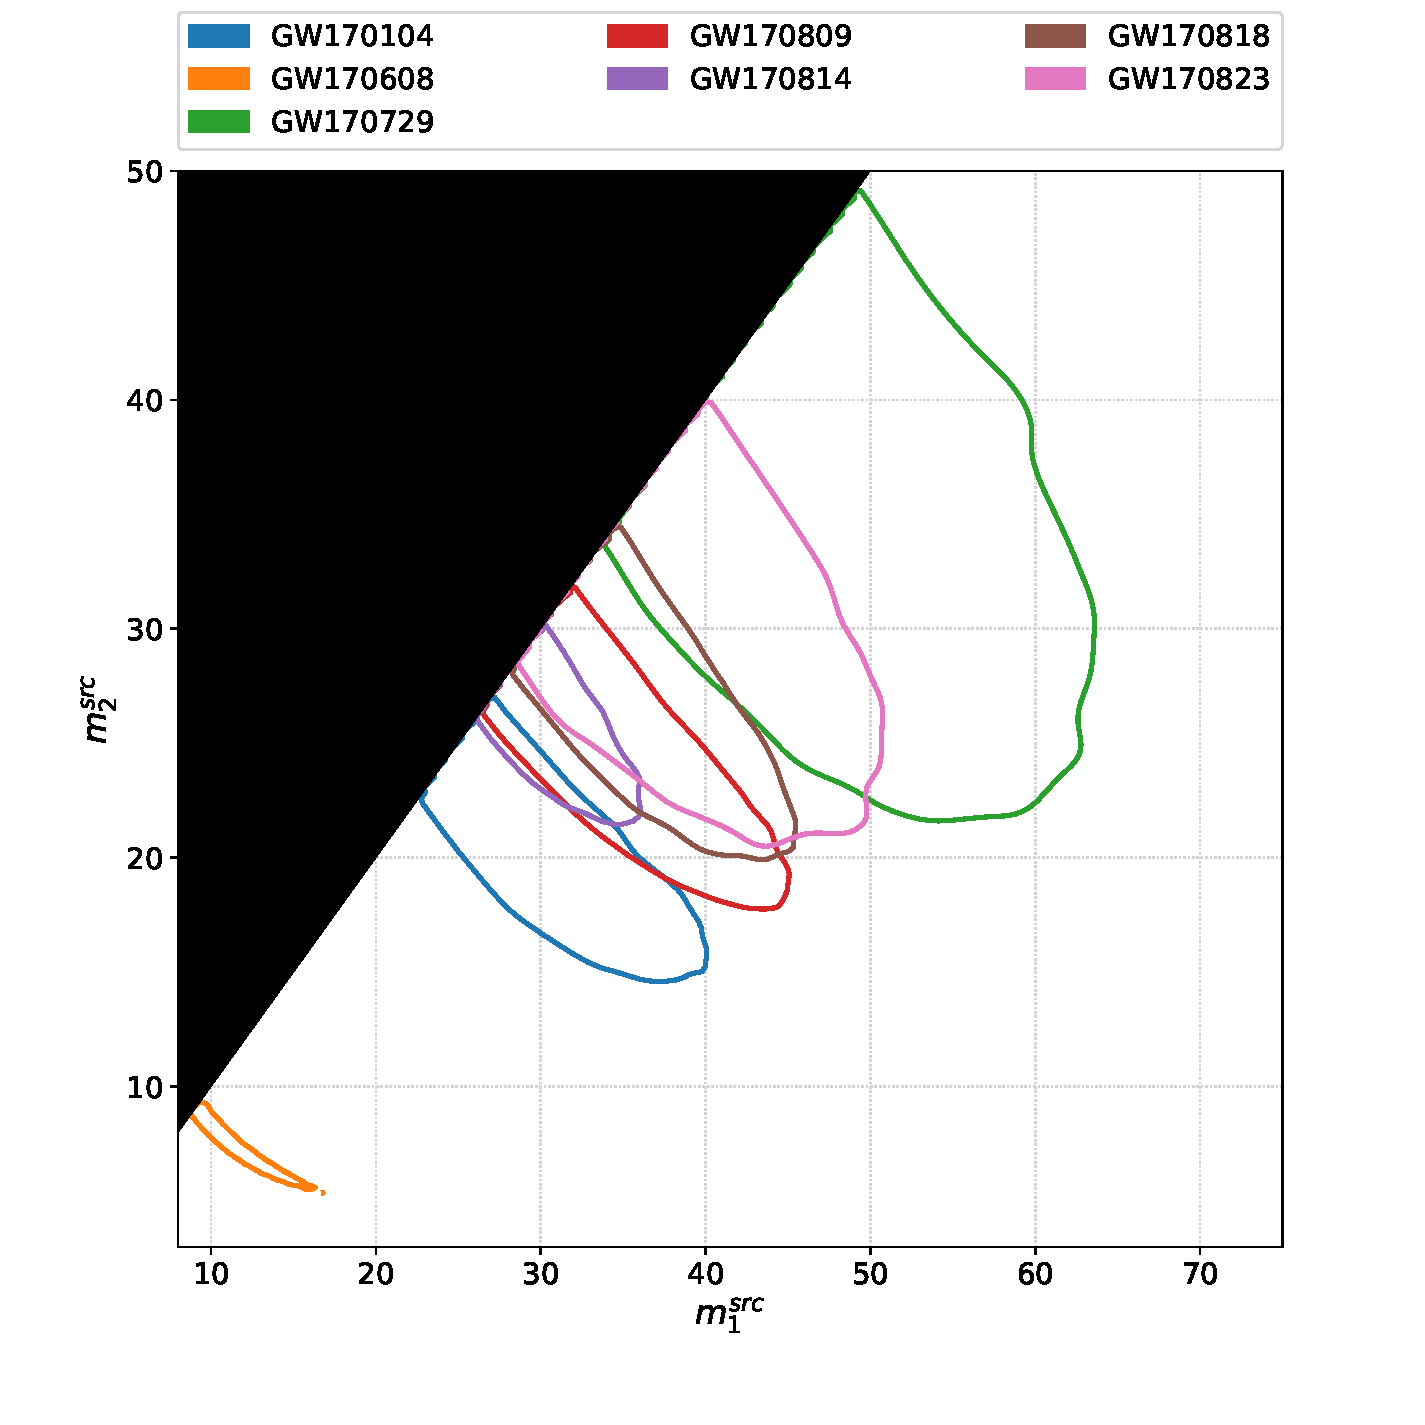
\includegraphics[width=\textwidth]{figures/o2_bbh_pe/all_o2_m1m2source.pdf}
  \caption{Posterior probabilities of the source frame primary mass $m_1^{\mathrm{src}}$ and secondary mass $m_2^{\mathrm{src}}$ from the PyCBC Inference analyses of the seven gravitational-wave signals from binary black-hole mergers in Advanced LIGO-Virgo's second observing run (O2). Plotted are the 90\% credible contours in the 2D plane. 
The measurements suggests that GW170729 has the highest masses and GW170608 has the lowest masses among all black hole binaries observed in O1 and O2. Parameter estimates of the O1 binary black holes were presented in Refs.~\cite{Biwer:2018osg,TheLIGOScientific:2016pea}.\label{fig:m1m2_plots}} 
\end{figure}

\begin{figure}[ht]
  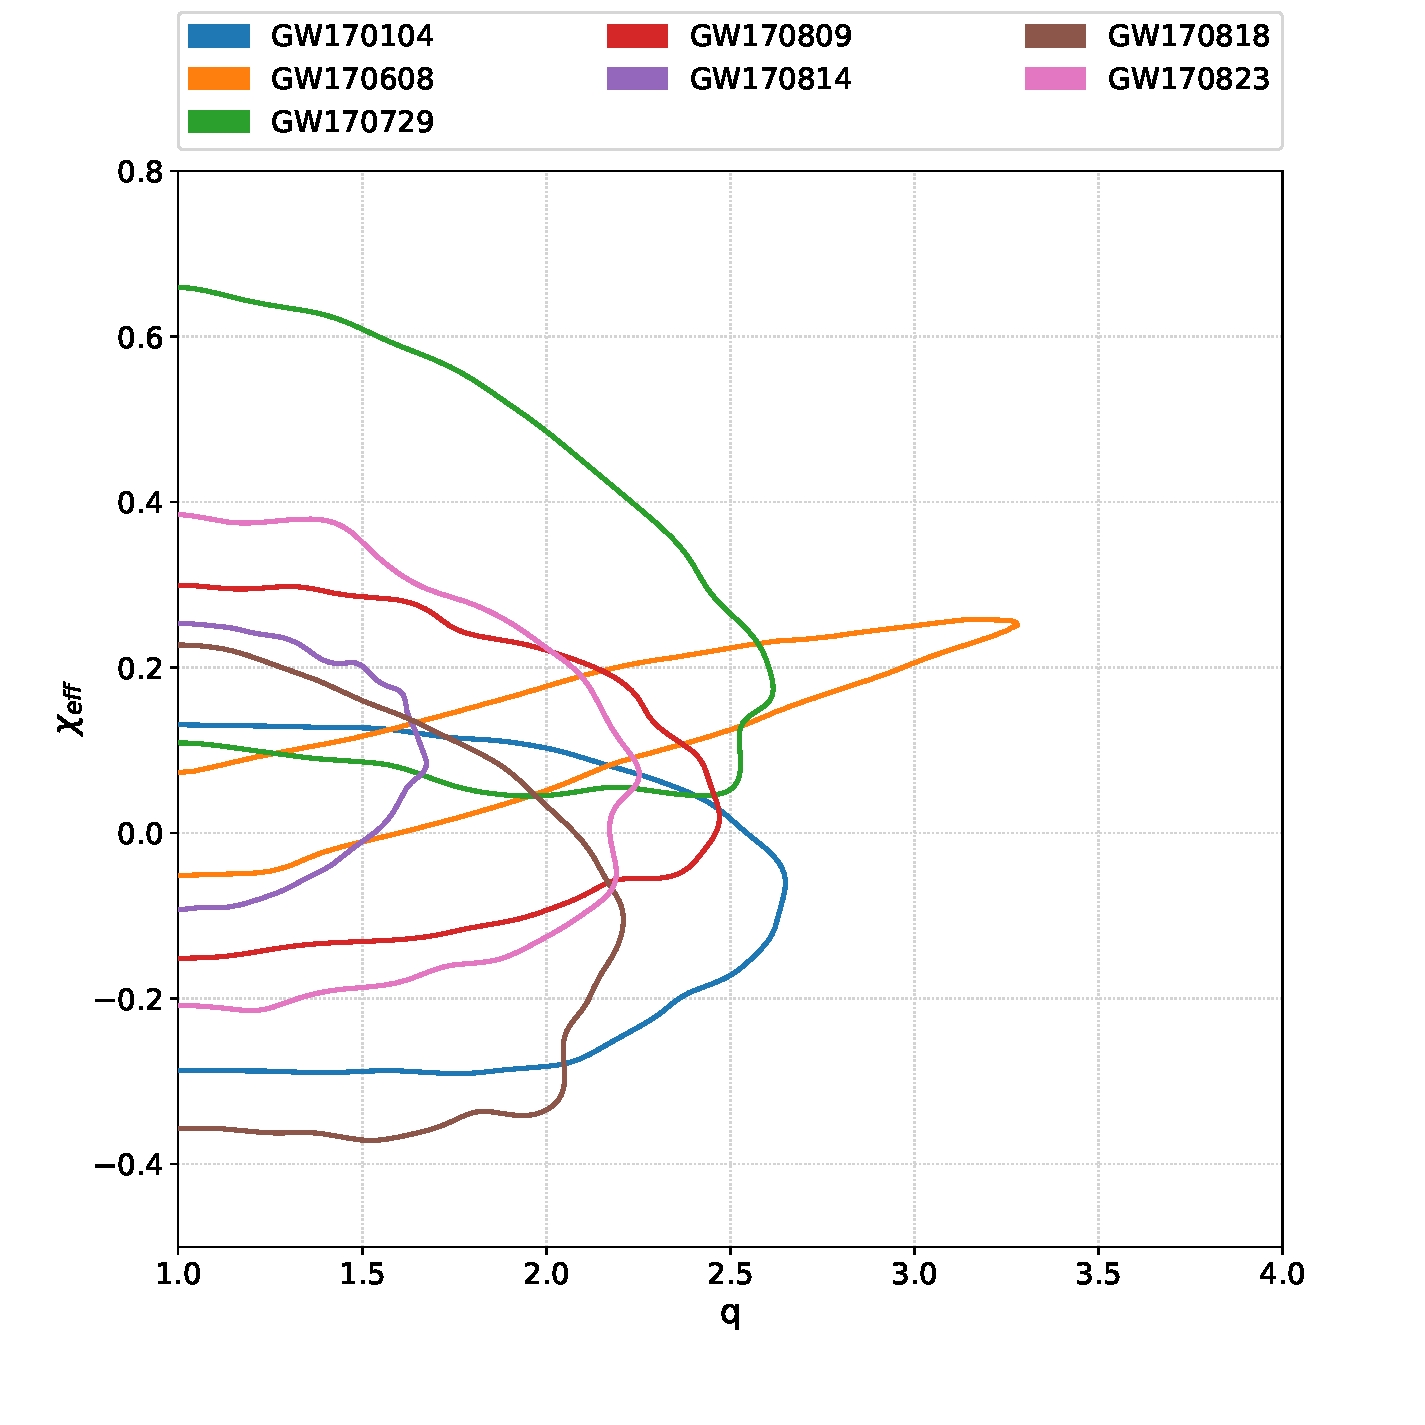
\includegraphics[width=\textwidth]{figures/o2_bbh_pe/all_o2_q_chieff.pdf}
  \caption{Posterior probabilities of the asymmetric mass ratio $q$ and the effective inspiral spin $\chi_{\mathrm{eff}}$ from the PyCBC Inference analyses of the seven gravitational-wave signals from binary black-hole mergers in Advanced LIGO-Virgo's second observing run. Plotted are the 90\% credible contours in the 2D plane. All the events have low $\chi_{\mathrm{eff}}$ values. GW170814 has lesser support for asymmetric mass ratios than the other events.
  \label{fig:qchieff_plots}
}
\end{figure}

\begin{figure}[ht]
  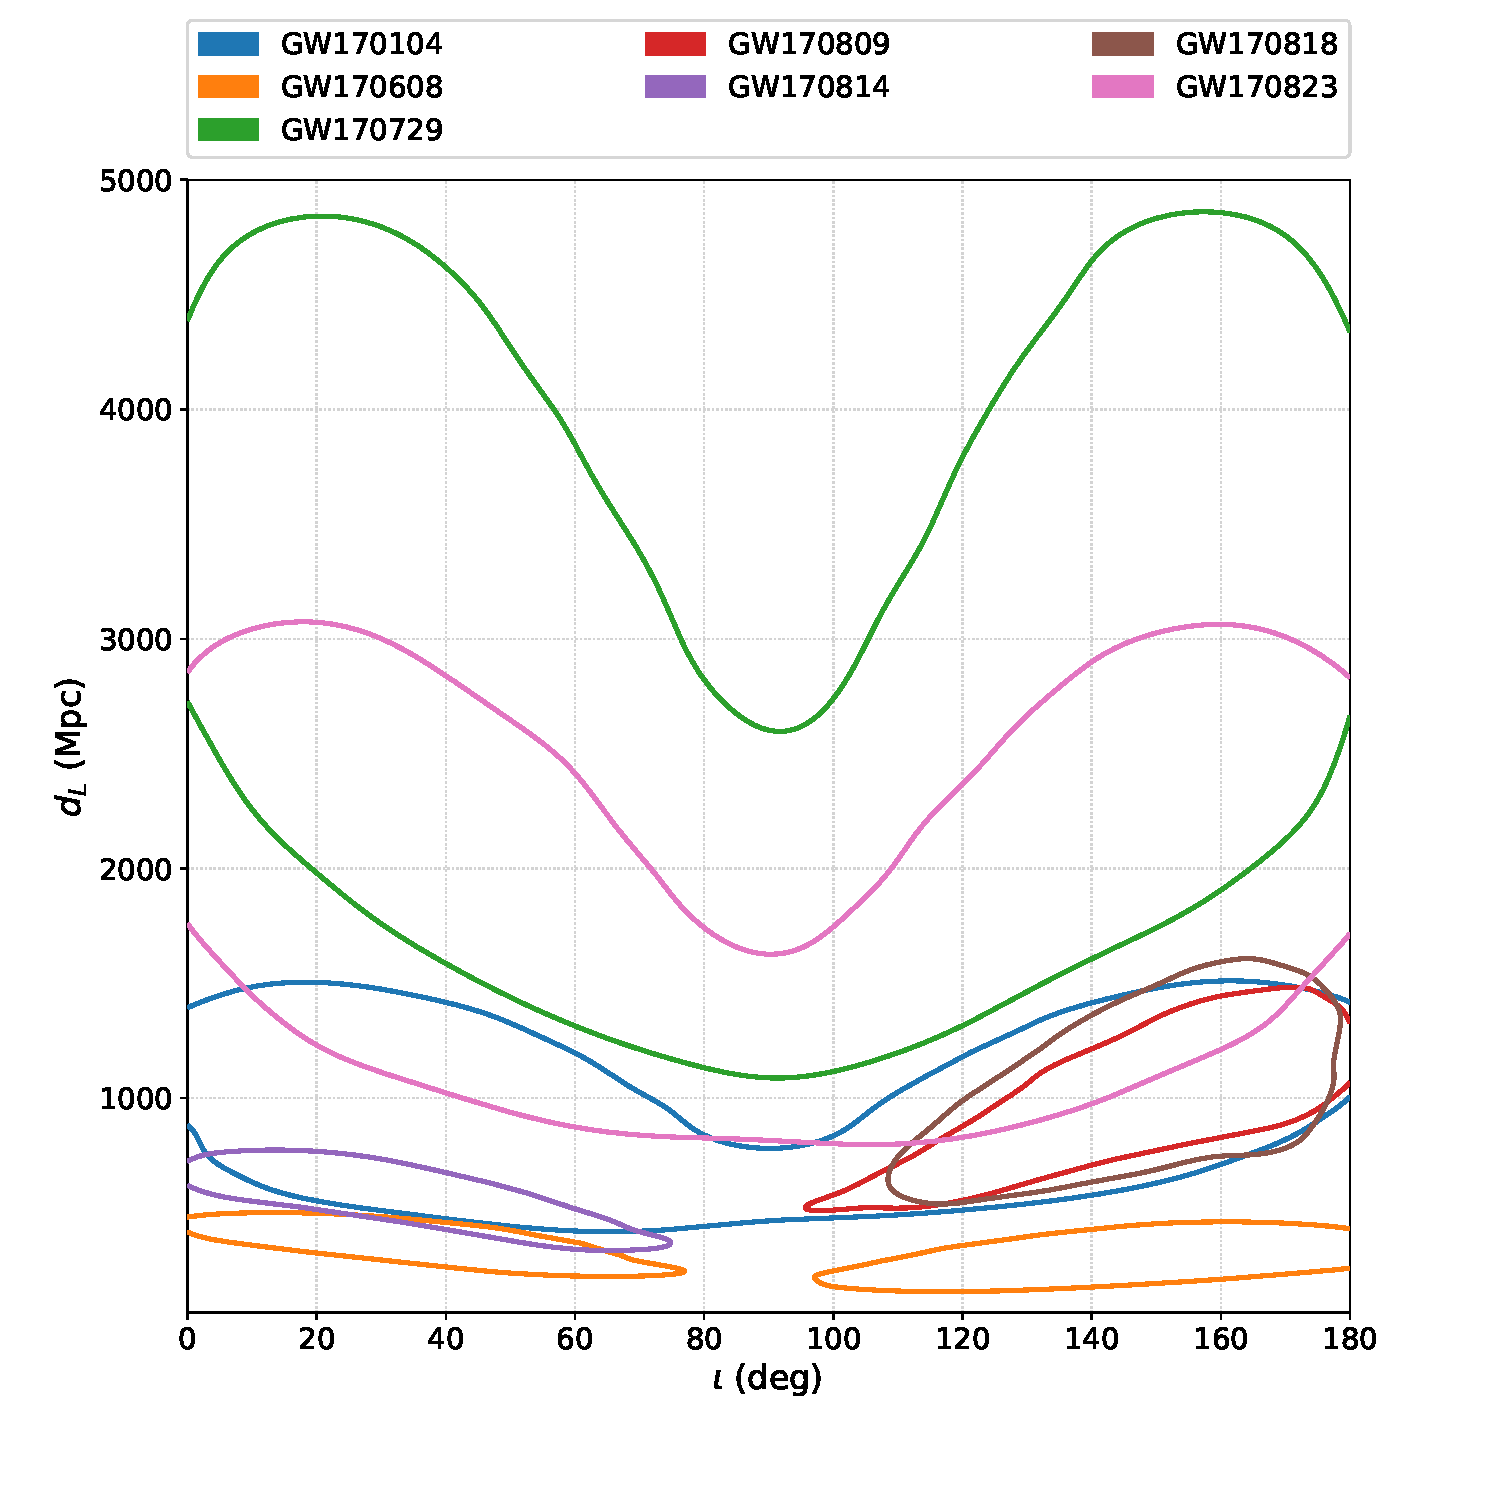
\includegraphics[width=\textwidth]{figures/o2_bbh_pe/all_o2_iota_dl.pdf}
  \caption{Posterior probabilities of the luminosity distance $d_L$ and the inclination angle $\iota$ from the PyCBC Inference analyses of the seven gravitational-wave signals from binary black-hole mergers in Advanced LIGO-Virgo's second observing run. Plotted are the 90\% credible contours in the 2D plane. GW170104, GW170729, and GW170823 have support for face-on ($\iota = 0$), face-off ($\iota = 180$) and edge-on ($\iota = 90$). For GW170608, there is a stronger preference for the system being face-on ($\iota = 0$) and face-off ($\iota = 180$). For GW170814, there is a stronger preference for the system being face-on ($\iota = 0$). For GW170809 and GW170818 there is a stronger preference for  face-off ($\iota = 180$). GW170608 is observed at the closest luminosity distance and GW170729 the farthest. \label{fig:dliota_plots}
}
\end{figure}


\begin{figure}[ht]
  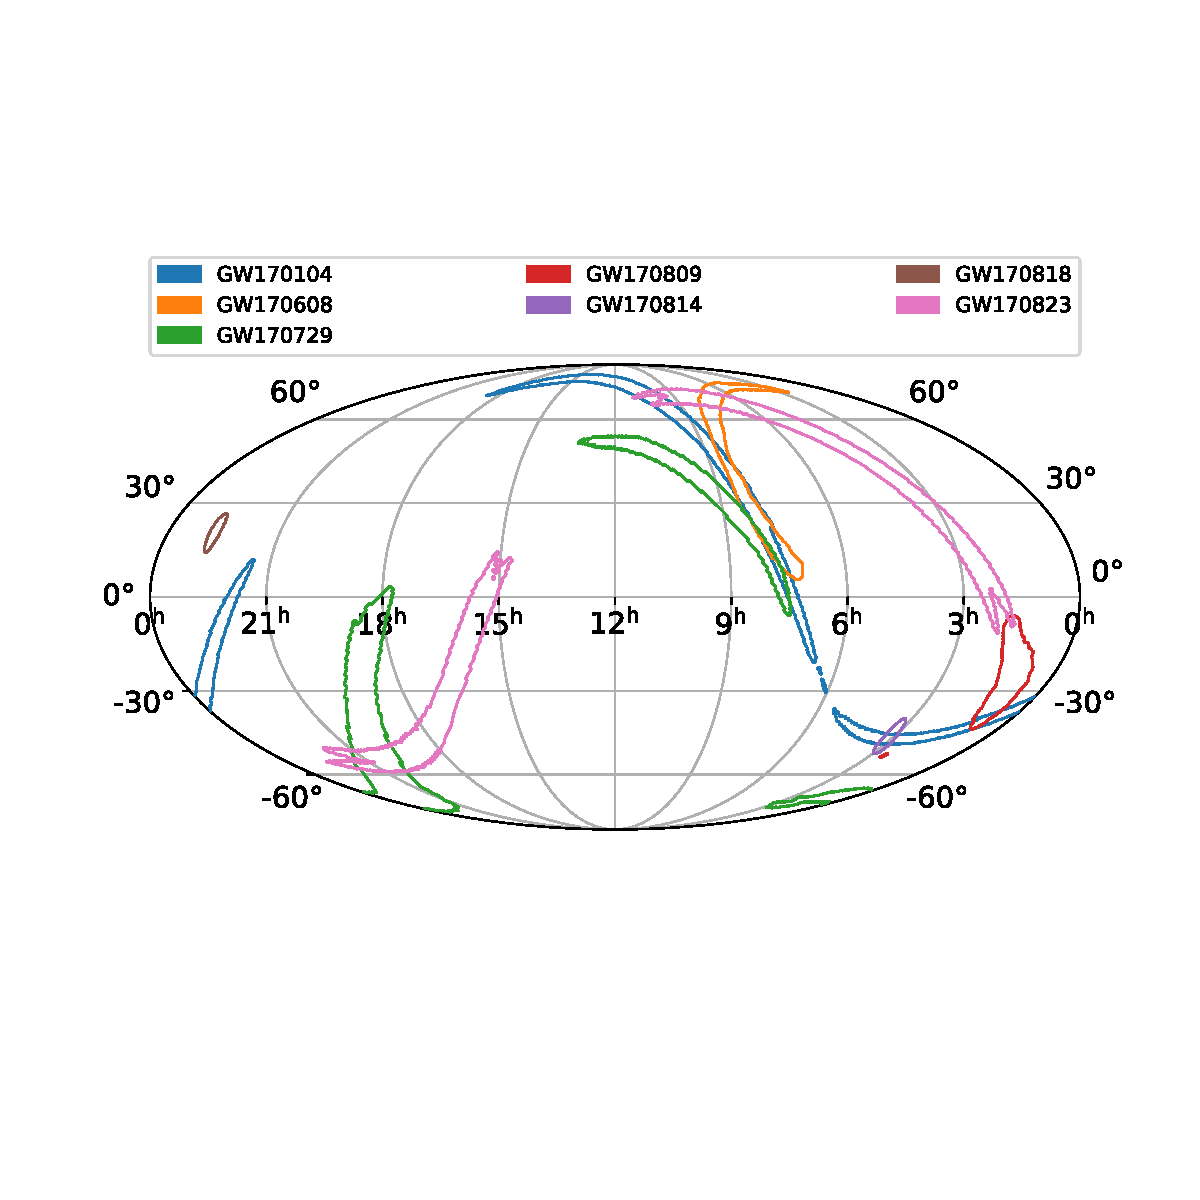
\includegraphics[width=\textwidth]{figures/o2_bbh_pe/all_o2_skymaps.pdf}
  \caption{Posterior probabilities for the sky location parameters---right ascension and declination from the PyCBC Inference analyses of the seven gravitational-wave signals from binary black-hole mergers in Advanced LIGO-Virgo's second observing run. Plotted are the 90\% credible contours in Mollweide projection and celestial coordinates; the right ascension is expressed in hours and the declination in degrees. GW170818 and GW170814 have substantially small sky localization areas, being detected by the H1L1V1 three-detector network, with considerable SNR in all the detectors. The GW170729 and GW170809 analyses used data from the three-detector network. However, the sky localization area is broad due to low Virgo SNR. Between GW170729 and GW170809, the latter has a higher network SNR leading to a smaller sky localization area. GW170104, GW170608, GW170823 have poor sky localization, as they were detected by the H1L1 two detector network; GW170823 has the lowest network SNR and broadest sky localization area, and GW170608 has the highest network SNR causing the smaller sky localization area. \label{fig:skymap_plots}
 }
\end{figure}


Estimates of the parameters for these events were previously published in the LIGO--Virgo Collaboration (LVC) detection papers for these events~\cite{Abbott:2017vtc,Abbott:2017gyy,Abbott:2017oio,LIGOScientific:2018mvr}. The results from our analyses are overall in agreement with the estimates published by the LVC within the statistical errors of measurement of the parameters. Any small discrepancies in the measurement of the parameters would be due to the differences in the analysis methods. One of the differences is the method of the PSD estimation. Another such difference is that we do not marginalize over calibration uncertainties of the measured strain~\cite{PhysRevD.96.102001}, whereas the LVC analyses use a spline model to fit the calibration uncertainties. The true impact of calibration errors on the parameter estimates should be evaluated using a physical model of the calibration, which does not exist currently in any analysis. This will be revisited in a future work.

\subsection{Code availability}
The posterior probability density functions presented in this paper were sampled using the PyCBC Inference software. The PyCBC Inference toolkit uses the Bayesian inference methodology described in this paper; a more detailed description of the toolkit is presented in Ref.~\cite{Biwer:2018osg}. The source code and documentation of PyCBC Inference is available as part of the PyCBC software package at \verb"http://pycbc.org". The results in this paper were generated with the PyCBC version 1.12.3 release. In the data release repository for this work~\cite{data_release} we provide scripts and configuration files for replicating our analysis. The scripts document our command line calls to the \texttt{pycbc\_inference} executable which performs the ensemble MCMC analyses. The command line call to \texttt{pycbc\_inference} contains options for: the ensemble MCMC configuration, data conditioning, and locations of the configuration file and gravitational-wave detector data files. The configuration files included in the repository, and used as an input to \texttt{pycbc\_inference}, specify the prior probability density functions used in the analyses, including sections for: initializing the distribution of Markov-chain positions in the ensemble MCMC, declaring transformations between the parameters that define the prior and the parameters the ensemble MCMC samples (eg. $(m_1, m_2) \rightarrow (\mathcal{M}, q)$), and defining additional constraints to the prior probability density function~\cite{Biwer:2018osg}.


\section{Data Records}\label{sec:data_record}

The data products from the parameter estimation analyses for the seven events are stored in seven HDF~\cite{andrew_collette_2018_1246321} files, available within the Zenodo data release repository~\cite{data_release} for this work. The location of these HDF files within the repository are listed in Table~\ref{tab:data_rec}. In this section, we describe the contents of these seven HDF files.

The top-level of the HDF files contains attributes named \texttt{ifos}, \texttt{variable\_args}, \texttt{posterior\_only}, and \texttt{lognl}. \texttt{variable\_args} is a list of the inferred model parameters.
For these seven analyses this includes: the coalescence time (\texttt{tc}), distance (\texttt{distance}), inclination angle (\texttt{inclination}), polarization angle (\texttt{polarization}), right ascension (\texttt{ra}), declination (\texttt{dec}), detector-frame component masses (\texttt{mass1} and \texttt{mass2}), azimuthal angles of the spin vector (\texttt{spin1\_azimuthal} and \texttt{spin2\_azimuthal}), polar angles of the spin vector (\texttt{spin1\_polar} and \texttt{spin2\_polar}), and magnitudes of the spin vector (\texttt{spin1\_a} and \texttt{spin2\_a}). \texttt{mass1}, \texttt{spin1\_a}, \texttt{spin1\_polar}, \texttt{spin1\_azimuthal} in the files refer to the primary black hole in the binary. \texttt{mass1}, \texttt{spin2\_a}, \texttt{spin2\_polar}, \texttt{spin2\_azimuthal} refer to the secondary black hole in the binary. 

\texttt{ifos} stores the list of the names of interferometers from which data has been analyzed in each run. The attribute \texttt{posterior\_only} is a Boolean where a \texttt{True} value indicates that the posterior samples and likelihood statistics are stored as flattened arrays in the files. \texttt{lognl} stores the value of the noise likelihood, which is described below.    
%Here, the label \texttt{1} (eg. \texttt{mass1} and \texttt{spin1\_a}) denotes the more massive black hole and the label \texttt{2} denotes the less massive black hole.

The independent samples of the model parameters are stored in a top-level HDF group, named \texttt{[`samples']}. For each parameter listed in the \texttt{variable\_args} attribute, the \texttt{[`samples']} HDF group contains an HDF dataset that is a one-dimensional array indexed by the independent samples. Therefore, the set of parameters for the $i$-th independent sample is the $i$-th element of each array. For example, \texttt{[`samples/mass1'][32]} and \texttt{[`samples/mass2'][32]} are the masses for the 32-nd independent sample. Samples in the \texttt{mass1} and \texttt{mass2} data sets are in solar mass units, those in \texttt{distance} are in Mpc units, those in \texttt{tc} are in seconds, and those in \texttt{spin1\_a} and \texttt{spin2\_a} are dimensionless. Samples in the \texttt{spin1\_polar}, \texttt{spin2\_polar}, \texttt{spin1\_azimuthal}, \texttt{spin2\_azimuthal}, \texttt{inclination}, \texttt{ra}, \texttt{dec}, and \texttt{polarization} are in radians.

%The azimuthal and polar angles of the spin vector are in spherical coordinates where $\theta^\mathrm{a}_{j} \in [0, 2 \pi)$ and $\theta^\mathrm{p}_{j} \in [0, \pi]$. The inclination angle is defined as: $\iota = 0$ is a ``face-on'' binary (line of sight parallel to binary angular momentum), $\iota = \pi / 2$ is an ``edge-on'' binary (line of sight perpendicular to binary angular momentum), and $\iota = \pi$ as a ``face-off'' binary (line of sight anti-parallel to binary angular momentum).

The second top-level HDF group is \texttt{[`prior\_samples']}, which stores prior samples in a similar format as the \texttt{[`samples']} group described above. For each of the parameters listed in the \texttt{variable\_args} attribute, the \texttt{[`prior\_samples']} HDF group contains an HDF dataset that is a one-dimensional array of samples of that parameter drawn from the prior distribution.

The third top-level HDF group, named \texttt{[`likelihood\_stats']}, contains quantities to obtain the prior $\prior$ and likelihood $\likelihood$ from Eq.~\ref{eqn:bayes} for each independent sample.
In order to obtain the prior for each independent sample, the \texttt{[`likelihood\_stats']} HDF group contains a dataset of the natural logarithm of the prior probabilities called \texttt{[`likelihood\_stats/prior']}. The datasets in the \texttt{[`likelihood\_stats']} HDF group are one-dimensional arrays indexed by the independent sample (eg. the $i$-th element corresponds to the prior probability of the $i$-th independent sample) as well. In order to obtain the likelihood for each independent sample, there is a dataset containing the natural logarithm of the likelihood ratio $\Lambda$ called \texttt{[`likelihood\_stats/loglr']}. The likelihood ratio $\Lambda$ is defined as~\cite{Biwer:2018osg}
\begin{equation}\label{eqn:lambda}
\log \Lambda = \log \frac{\likelihood}{p(\vec{d}(t)|\vec{n})}
\end{equation}
where $\log p(\vec{d}(t)|\vec{n})$ is the natural logarithm of the noise likelihood defined as~\cite{Biwer:2018osg}
\begin{equation}\label{eqn:noise_likelihood}
\log p(\vec{d}(t)|\vec{n}) = - \frac{1}{2} \sum_{i=1}^{N} \left< \tilde{d}_{i}(f) | \tilde{d}_{i}(f) \right> \,.
\end{equation}
The natural logarithm of the noise likelihood is a constant for each analysis. Therefore from Eq.~\ref{eqn:lambda}, in order to compute the natural logarithm of the likelihood, $\log \likelihood$, the user adds \texttt{lognl} to each element of \texttt{[`likelihood\_stats/loglr']}.

The fourth top-level HDF group is \texttt{[`psds']}. For each interferometer from which data has been used in the analysis, the \texttt{[`psds']} HDF group contains a dataset storing a frequency series of the PSD multiplied by the square of the dynamic range factor. The dynamic range factor is a large constant to reduce the dynamic range of the strain; here, we use $2^{69}$ rounded to 17 significant figures (precisely $5.9029581035870565\times 10^{20}$). The first entry in each PSD frequency series corresponds to frequency $f = 0$~Hz, and the last entry corresponds to $f = 1024$~Hz. Attached as attributes to each interferometer's PSD frequency series dataset object are the frequency resolution---\texttt{delta\_f} and the low frequency cutoff used for that interferometer in the PSD estimation and likelihood computation---\texttt{low\_frequency\_cutoff}.

\vspace{0.5cm}
\begin{table*}[t]
\begin{adjustwidth}{-0.3cm}{}
\begin{tabular}{ |p{2cm}||p{1.5cm}|p{11cm}|  }
 \hline
 Event & Posterior samples & Location of the associated data file within the data release repository \\
 \hline
 \hline
 GW170104 & 8000 & \verb"posteriors/GW170104/gw170104_posteriors_thinned.hdf" \\
 \hline
 GW170608 & 8000 & \verb"posteriors/GW170608/gw170608_posteriors_thinned.hdf" \\
 \hline 
 GW170814 & 8000 & \verb"posteriors/GW170814/gw170814_posteriors_thinned.hdf" \\
 \hline
 GW170729 & 8000 & \verb"posteriors/GW170729/gw170729_posteriors_thinned.hdf" \\
 \hline
 GW170809 & 8000 & \verb"posteriors/GW170809/gw170809_posteriors_thinned.hdf" \\
 \hline
 GW170818 & 8000 & \verb"posteriors/GW170818/gw170818_posteriors_thinned.hdf" \\
 \hline
 GW170823 & 8000 & \verb"posteriors/GW170823/gw170823_posteriors_thinned.hdf" \\
 \hline
\end{tabular}
\caption{For each binary black hole merger, this table contains: the event's name, number of independent samples obtained with the ensemble MCMC, and location of the HDF files containing the independent samples within the Zenodo data release repository~\cite{data_release}.\label{tab:data_rec}}
\end{adjustwidth}
\end{table*}
\vspace{0.5cm}


\section{Technical Validation}\label{sec:validation}

The analyses in this paper were performed using the PyCBC Inference software~\cite{Biwer:2018osg} with the parallel-tempered emcee sampler~\cite{emcee,mcmc} \newline (\verb"https://github.com/dfm/emcee/tree/v2.2.1"), hereafter referred to as \texttt{emcee\_pt}, as the sampling algorithm. A validation study of PyCBC Inference with the \texttt{emcee\_pt} sampler was presented in Sec.~4 of Ref.~\cite{Biwer:2018osg}. The validation study in Ref.~\cite{Biwer:2018osg} used the same version of the PyCBC code, waveform model, sampler settings, data conditioning settings, and burn-in test as used in our analyses in this paper, and therefore demonstrates the credibility of the results presented in this paper. In this section, we summarize the validation study.

We have tested the performance of this setup (ie. code version, waveform model, sampler settings, etc.) using analytic likelihood functions such as the multivariate normal, Rosenbrock, eggbox, and volcano functions. The \texttt{emcee\_pt} sampler successfully sampled the underlying analytical distributions. The recovery of parameters of a four-dimensional normal distribution using the \texttt{emcee\_pt} sampler is shown in Fig.~2 of Ref.~\cite{Biwer:2018osg}.

Ref.~\cite{Biwer:2018osg} also describes a test performed using simulated binary black hole signals to validate the reliability of parameter estimates generated by PyCBC Inference with the \texttt{emcee\_pt} sampler. The test is carried out by generating 100 realizations of stationary Gaussian noise colored by the power spectral densities of the Advanced LIGO detectors around the time of observation of GW150914~\cite{Abbott:2016blz}. A unique simulated binary black hole signal, whose parameters were sampled from the prior probability density function, is injected into each simulated noise realization. For the population of 100 simulated binary black hole signals, the network signal-to-noise ratios range from 5 to 160, and are predominantly spaced between 10 to 40. PyCBC Inference, using the \texttt{emcee\_pt} sampler, was then run on each simulated binary black hole signal to produce samples of the posterior probability density function and compute credible intervals that estimate the modeled parameter values. For each parameter, we then calculate the percentage of the runs ($x\%$) in which the true value of the parameter was recovered within a certain credible interval ($y\%$). In the ideal case, there should be a 1-to-1 relation between these percentiles, ie. $x$ should equal $y$ for any value of the percentile $y$. The percentile-percentile curves obtained for each parameter in the test is plotted in Fig.~3 of Ref.~\cite{Biwer:2018osg}. To evaluate the deviation between the percentile-percentile curve for each parameter from a 1-to-1 relation, a Kolmogorov-Smirnov (KS) test is performed. Using the set of p-values obtained for all the parameters, another KS test is performed expecting the p-values to adhere to a uniform distribution. The p-value obtained from this calculation is 0.7, which is sufficiently high to infer that PyCBC Inference, with it's implementation of the \texttt{emcee\_pt} sampler, provides unbiased estimates of the binary black hole modeled parameters.

In addition to the aforementioned tests using analytical distributions and simulated signals, the 90\% credible interval measurements of the binary black hole parameters from our analyses presented in this paper are in agreement with the LIGO--Virgo Collaboration estimates~\cite{Abbott:2017vtc,Abbott:2017gyy,Abbott:2017oio} which used a different inference code. This further validates the results presented here.

\section{Usage Notes}\label{sec:con}
%When citing the data associated with this paper and released in the data release repository~\cite{data_release}, please cite this paper for describing the data and the analyses that generated them. Please also cite Ref.~\cite{Biwer:2018osg} which describes and validates the PyCBC Inference parameter estimation toolkit that was used for generating the data. 
The samples of the posterior probability density function for each analysis presented in this work are stored in separate HDF files, and the location of each HDF file is listed in Table~\ref{tab:data_rec}. We direct users to the tools available in PyCBC Inference to read these files and visualize the data. Figs.~\ref{fig:m1m2_plots}, \ref{fig:qchieff_plots}, and \ref{fig:dliota_plots} in this paper were generated using these tools from the PyCBC version 1.12.3 release. The data release repository also includes scripts to execute \texttt{pycbc\_inference} and reproduce the analysis and resulting samples.

The data release repository for this work~\cite{data_release} includes two IPython notebooks named \verb"data_release_o2_bbh_pe.ipynb" and \verb"o2_bbh_pe_skymaps.ipynb". \newline
\verb"data_release_o2_bbh_pe.ipynb" presents tutorials for using PyCBC to handle the data. This notebook contains examples to load the HDF datasets, convert the parameters in the HDF files to other coordinates (eg. $(m_1^{\mathrm{det}}, m_2^{\mathrm{det}}) \rightarrow (\mathcal{M}^{\mathrm{det}}, q)$), and visualize the samples of the posterior probability density function. The samples' credible intervals are visualized as marginalized one-dimensional histograms and two-dimensional credible contour regions. We include commands in this notebook to reproduce Figs.~\ref{fig:m1m2_plots}, \ref{fig:qchieff_plots}, and~\ref{fig:dliota_plots} in this paper.
PyCBC Inference also includes an executable called \texttt{pycbc\_inference\_plot\_posterior} to render these visualizations. 
The IPython notebook \verb"o2_bbh_pe_skymaps.ipynb" demonstrates a method of visualizing the sky location posterior distributions, as presented in Fig.~\ref{fig:skymap_plots} in this paper. We use tools from the open source ligo.skymap package (\verb"https://pypi.org/project/ligo.skymap/") for writing the sky location posterior samples from our analyses into FITS files, reading them, and generating probability density contours on a Mollweide projection.
\Chapter{Tidal Deformabilities and Radii of Neutron Stars from the Observation of GW170817}
\label{ch:common_eos}
We use gravitational-wave observations of the binary neutron star merger GW170817 to explore the tidal deformabilities and radii of neutron stars.
We perform Bayesian parameter estimation with the source location and distance informed by electromagnetic observations. We also assume that the two stars have the same equation of state; we demonstrate that for stars with masses comparable to the component masses of GW170817, this is effectively implemented by assuming that the stars' dimensionless tidal deformabilities are determined by the binary's mass ratio $q$ by $\Lambda_1/\Lambda_2 = q^6$. We investigate different choices of prior on the component masses of the neutron stars. We find that the tidal deformability and 90\% credible interval is $\tilde{\Lambda}=222^{+420}_{-138}$ for a uniform component mass prior, $\tilde{\Lambda}=245^{+453}_{-151}$ for a component mass prior informed by radio observations of Galactic double neutron stars, and $\tilde{\Lambda}=233^{+448}_{-144}$ for a component mass prior informed by radio pulsars. We find a robust measurement of the common areal radius of the neutron stars across all mass priors of $8.9 \le \hat{R} \le 13.2$~km, with a mean value of $\langle \hat{R} \rangle = 10.8$~km. Our results are the first measurement of tidal deformability with a physical constraint on the star's equation of state and place the first lower bounds on the deformability and areal radii of neutron stars using gravitational waves.

\section{Introduction}

On August 17, 2017 LIGO and Virgo observed gravitational waves from a binary neutron star coalescence, GW170817~\cite{TheLIGOScientific:2017qsa}.
This observation can be used to explore the equation of state (EOS) of matter at super-nuclear densities~\cite{thorne.k:1987,Read:2009yp}. In a neutron star binary, as the two components come in close vicinity to each other at the end of their inspiral phase, the tidal field of each neutron star induces a quadrupolar deformation in the structure of its companion. The deformation of each component object can be characterized by a parameter called the tidal deformability, $\lambda$, related to the star's quadrupolar deformation $Q_{ij}$ and its companion's tidal field $\epsilon_{ij}$ as $Q_{ij} = -\lambda \epsilon_{ij}$, with $i \in \{1,2\}$ being indices denoting the two stars. The tidal deformability of each star depends on the mass and radius of the star, and the nuclear equation of state. In dimensionless form, the deformability of each star can be written as
\begin{equation}
\Lambda_{1,2}=\frac{2}{3}k_2\left(\frac{R_{1,2}c^2}{Gm_{1,2}}\right)^5, \label{eq:lambda_12}
\end{equation}
where $k_2$ is the tidal Love number~\cite{Flanagan:2007ix,Hinderer:2007mb}, which depends on the star's mass and the EOS. $R_{1,2}$ and $m_{1,2}$ are the areal radii and masses of the neutron stars, respectively. The tidal deformabilities are encoded as a change in the phase evolution of the gravitational wave emitted by the binary~\cite{Flanagan:2007ix}. %This information is encoded as a change in gravitational-wave phase evolution caused by the tidal deformation of the  neutron stars~\cite{Flanagan:2007ix}. 
At leading order, the tidal effects are imprinted in the gravitational-wave signal through the binary tidal deformability~\cite{Flanagan:2007ix,Hinderer:2007mb}
\begin{equation}
\tilde{\Lambda}
= \frac{16}{13}\frac{(12q+1)\Lambda_1+(12+q)q^4\Lambda_2}{(1+q)^5}, \label{eq:lambda_t0}
\end{equation}
where $q = m_2/m_1 \leq 1$ is the binary's mass ratio [cf. Eq.~(34) of Ref.~\cite{Gralla:2017djj}]. %The deformability of each star is
%\begin{equation}
%\Lambda_{1,2}=\frac{2}{3}k_2\left(\frac{R_{1,2}c^2}{Gm_{1,2}}\right)^5, \label{eq:lambda_12}
%\end{equation}
%where $k_2$ is the tidal Love number~\cite{Flanagan:2007ix,Hinderer:2007mb}, which depends on the star's mass and the EOS. $R_{1,2}$ and $m_{1,2}$ are the areal radii and masses of the neutron stars, respectively. 

In the results of Ref.~\cite{TheLIGOScientific:2017qsa},
the priors on $\Lambda_{1,2}$ are taken to be completely uncorrelated,
which is equivalent to assuming that each star may have a different
EOS. Here, we reanalyze the gravitational-wave data using Bayesian
inference \cite{Biwer:2018osg,alex_nitz_2018_1208115,emcee} to measure the tidal deformability, using a
correlation between $\Lambda_1$ and $\Lambda_2$ which follows from the
assumption that both stars have the same EOS.  We repeat
our analysis without the common EOS constraint and calculate the 
Bayes factor that compares the evidences for these two models.
We also fix the sky position and
distance from electromagnetic observations~\cite{Soares-Santos:2017lru,Cantiello:2018ffy}.
We study the effect of
the prior for the component masses by performing analyses with three
different priors: the first is uniform between 1 and $2M_\odot$, the
second is informed by radio observations of double neutron star
binaries, and the third is informed by the masses of isolated pulsars~\cite{Ozel:2016oaf}.

\section{The common equation of state constraint}\label{sec:ceos_constraint}

To explore imposing a common EOS constraint, we employ a piecewise polytrope scheme ~\cite{Lattimer:2015nhk} to simulate thousands of equations of state.  Each EOS obeys causality, connects at low densities to the well-known EOS of neutron star crusts~\cite{Lattimer:2012nd}, is constrained by experimental and theoretical studies of the symmetry properties of matter near the nuclear saturation density, and satisfies the observational constraint for the maximum mass of a neutron star, $m_\mathrm{max}\ge2M_\odot$~\cite{Antoniadis:2013pzd}. Figure~\ref{fig:lam-mass} shows the results of Tolman-Oppenheimer-Volkoff (TOV) integrations~\cite{Oppenheimer:1939ne,Postnikov:2010yn} to determine $\Lambda$ as functions of $m$, $R$, and the EOS. Each configuration is color coded according to its
radius. In the relevant mass range, $\Lambda$ generally varies as
$m^{-6}$. For a given mass $m$, there is an inherent spread of about a factor of ten in $\Lambda$, which is correlated with $R^6$. We find that the star's tidal deformability is related to its compactness parameter 
$\beta=Gm/(Rc^2)$ by the relation $\Lambda~\simeq a\beta^{-6}$. We find that $a=0.0093\pm0.0007$ bounds this relation if $1.1M_\odot\le m\le1.6M_\odot$
(note that this is a bound, not a confidence interval). The additional power of $\beta^{-1}$ in the $\Lambda-\beta$ relation, relative to $\beta^{-5}$ in Eq.~(\ref{eq:lambda_12}), originates because the dimensionless tidal Love number, $k_2$, varies roughly as $\beta^{-1}$ for masses $\geq$
$1M_\odot$, although this is not the case for all masses~\cite{Postnikov:2010yn}. For $m\to0$ we see that $k_2\to0$ so that $k_2$ is proportional to $\beta$ with a positive power, but since neutron stars with $m < 1\,M_\odot$ are physically unrealistic, that domain is not pertinent to this Letter.

We observed that, for nearly every specific EOS, the range of stellar radii in the mass range of interest for GW170817 is typically small. As long as $m_{\rm max}\ge 2M_\odot$, the piecewise polytrope study reveals $\langle \Delta R \rangle =-0.070$ km and $\sqrt{\langle(\Delta R)^2\rangle}~=0.11$ km, where $\Delta R \equiv R_{1.6}-R_{1.1}$ with $R_{1.1,1.6}$ the radii of stars with $m=1.1$ and $m=1.6M_\odot$, respectively. Therefore, for masses relevant for GW170817, each EOS assigns a common value of $\hat R$ to stellar radii with little sensitivity to the mass. We can combine the relations $\Lambda~\simeq a\beta^{-6}$ and $R_1=R_2$ to find the simple prescription $\Lambda_1=q^6\Lambda_2$. We impose the common EOS constraint in our analysis using this relation. The exponent of $q$ changes with chirp mass $\mathcal{M}$ and for $\mathcal{M} > 1.5\,M_\odot$ this relation has to be modified. However, this is not relevant for the study of GW170817.

\begin{figure}[t]
  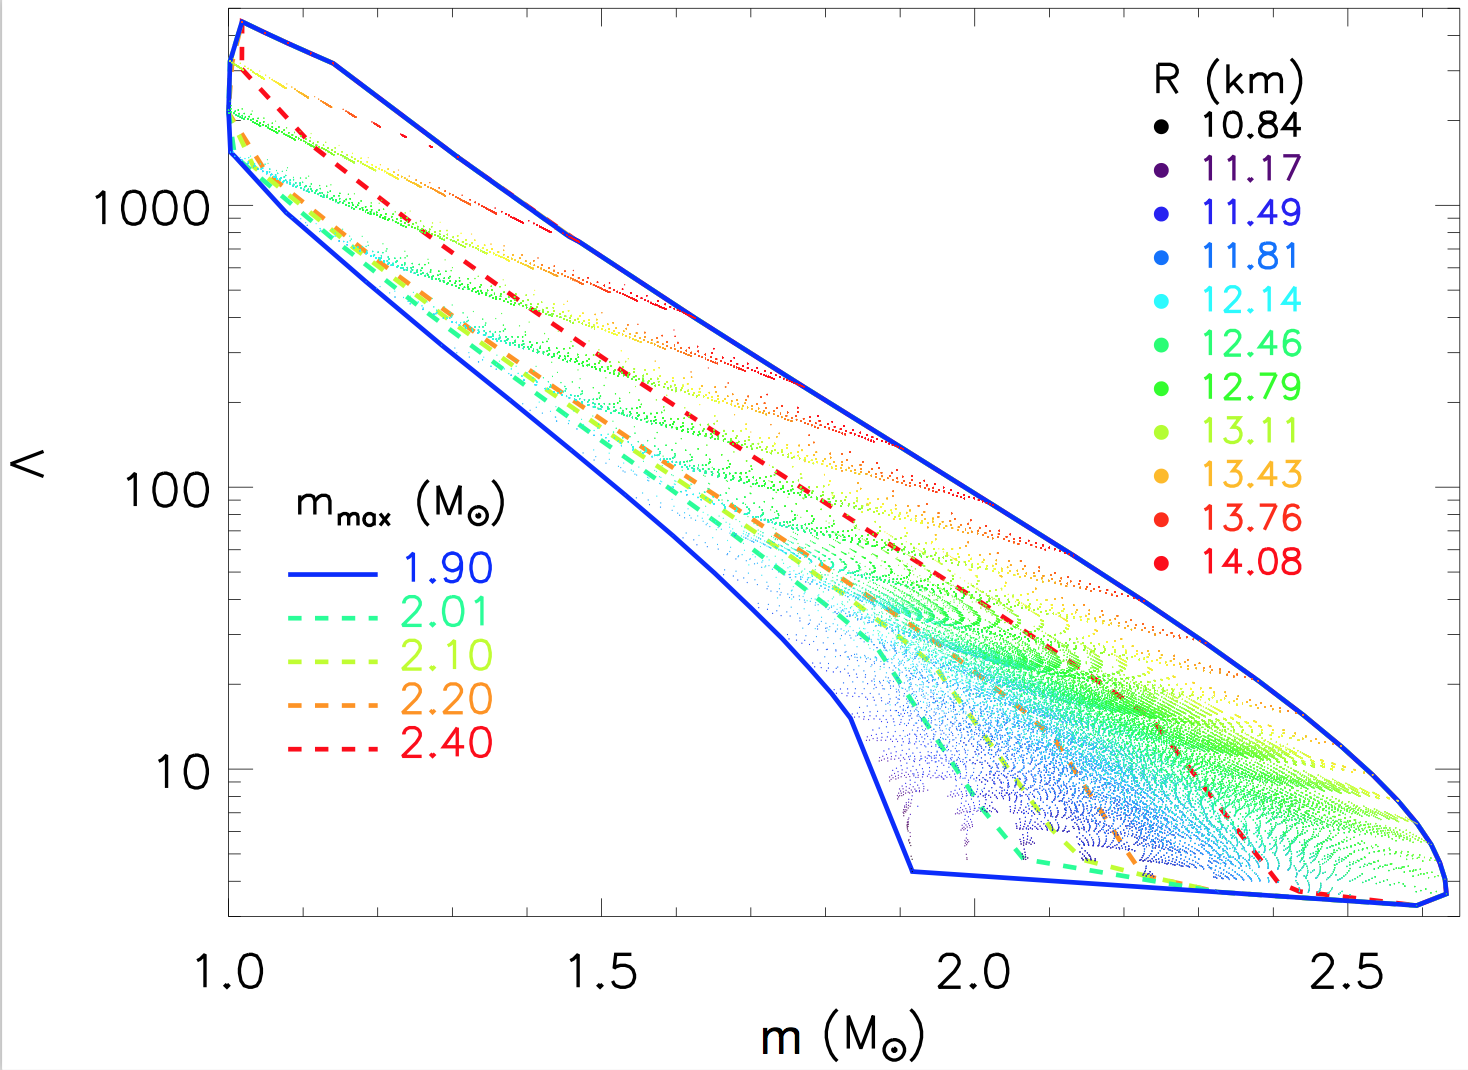
\includegraphics[width=\columnwidth]{figures/common_eos/lam-mass.png}
  \caption{The tidal deformability $\Lambda$ as a function of mass for physically realistic polytropes. A TOV integration with each EOS parameter set results in a series of values of $\Lambda(m)$ that are shown as points colored by their radii $R$. Dashed curves are lower bounds to $\Lambda$ for a given mass $m$ which vary depending on the assumed lower limit to the neutron star maximum mass, $m_\mathrm{max}$.  All values of $m_\mathrm{max}$ produce the same upper bound. \label{fig:lam-mass}}
\end{figure}



\section{Implications for the neutron star radius}

The common EOS constraint allows us to show that the binary tidal deformability $\tilde\Lambda$ is essentially a function of the chirp mass ${\cal{M}}$, the common radius $\hat R$, and the mass ratio $q$, but that its dependence on $q$ is very weak. Substituting the expressions $\Lambda~\simeq a\beta^{-6}$ and $R=\hat R$ into Eq. (\ref{eq:lambda_t0}), we find
\begin{equation}
\tilde{\Lambda}=
\frac{16a}{13}
\left(
\frac{\hat{R}c^2}{G{\cal M}}
\right)^6 f(q).
\label{eq:lambda_t1}\end{equation}
where $f(q)$ is very weakly dependent on $q$:
\begin{equation}
f(q)=q^{8/5}(12-11q+12q^2)(1+q)^{-26/5}.
\end{equation}
For example, if we compare a binary with $q = 0.75$ to an equal mass binary, we find $f(0.75)/f(1)=1.021$. As long as $q\ge0.6$, valid for $1M_\odot\le m\le 1.6 M_\odot$ for both stars, we infer from Eq.~(\ref{eq:lambda_t1}),
\begin{equation}
\tilde{\Lambda}=a^\prime\left(\frac{\hat{R}c^2}{G{\cal M}}\right)^6,
\label{eq:lambda_t2}\end{equation}
where $a^\prime=0.0042\pm0.0004$. Section \ref{sec:ceos_radius} shows TOV integrations for a range of EOS that validate this relationship. For stars with masses comparable to GW170817, the common radius $\hat R$ can be found from the inversion of Eq. (\ref{eq:lambda_t2}),
\begin{equation}
\hat R\simeq R_{1.4}\simeq (11.2\pm0.2)\frac{\cal M}{M_\odot}\left(\frac{\tilde{\Lambda}}{800}\right)^{1/6}{\rm~km}.
\label{eq:rhat}\end{equation}
The quoted errors originate from the uncertainties in $a$ and $q$, and amount, in total, to 2\%.

\section{Parameter estimation}
\subsection{Summary of methods}\label{sec:pe_methods_ceos_summ}
We use Bayesian inference to measure the parameters of GW170817 \cite{Christensen:2001cr}. We calculate the posterior probability density function, $p(\vec{\theta}|\vec{d}(t),H)$, for the set of parameters $\vec{\theta}$ for the gravitational-waveform model, $H$, given the LIGO Hanford, LIGO Livingston, and Virgo data $\vec{d}(t)$~\cite{Vallisneri:2014vxa,gw170817-losc}
\begin{equation}
p(\vec{\theta}|\vec{d}(t),H) = \frac{p(\vec{\theta}|H) p(\vec{d}(t)|\vec{\theta},H)}{p(\vec{d}(t)|H)}.
\label{eq:postpdf}
\end{equation}
The prior, $p(\vec{\theta}|H)$, is the set of assumed probability distributions for the waveform parameters. The likelihood $p(\vec{d}(t)|\vec{\theta},H)$ assumes a Gaussian model for the detector noise~\cite{Rover:2006bb}. Marginalization of the likelihood to obtain the posterior probabilities is performed using Markov Chain Monte Carlo (MCMC) techniques using the PyCBC inference software \cite{Biwer:2018osg,alex_nitz_2018_1208115} and the parallel-tempered EMCEE sampler \cite{emcee,vousden:2016,mcmc}. We fix the sky location and distance to GW170817~\cite{Soares-Santos:2017lru,Cantiello:2018ffy} and calculate the posterior probabilities for the remaining source parameters. Following Ref.~\cite{TheLIGOScientific:2017qsa}, the waveform model $H$ is the restricted TaylorF2 post-Newtonian aligned-spin model \cite{Sathyaprakash:1991mt,Buonanno:2009zt,Arun:2008kb,Mikoczi:2005dn,Bohe:2013cla,Vines:2011ud}.
Technical details of our parameter estimation and a comparison to Fig.~5 of Ref~\cite{TheLIGOScientific:2017qsa} are provided in Section \ref{sec:pe_methods_ceos_tech_details}.%as Supplemental Material~\cite{supp}.

To implement the common EOS constraint we construct the priors on $\Lambda_{1,2}$ according to
\begin{equation}
\Lambda_1=q^3\Lambda_s,\qquad\Lambda_2=q^{-3}\Lambda_s,
\label{eq:lambdas}\end{equation}
where $\Lambda_s \sim U[0,5000]$. We discard draws with 
$\tilde{\Lambda} > 5000$, since these values are beyond the range of all plausible EOS. The resulting prior on $\tilde\Lambda$ is uniform between $0$ and $5000$.  We also perform analyses that do not assume the common EOS constraint where we allow completely uncorrelated priors for $\Lambda_{1,2}$. This allows us to compare the evidences between these hypotheses. For the uncorrelated $\Lambda_{1,2}$ analyses, the prior for $\Lambda_1 \sim U[0,1000]$ and $\Lambda_2 \sim U[0,5000]$ with these intervals set by the range of plausible equations of state in the mass range of interest, our convention of $m_1 \geq m_2$, and discarding draws with $\tilde\Lambda > 5000$.

\iffalse
\begin{figure*}[t]
  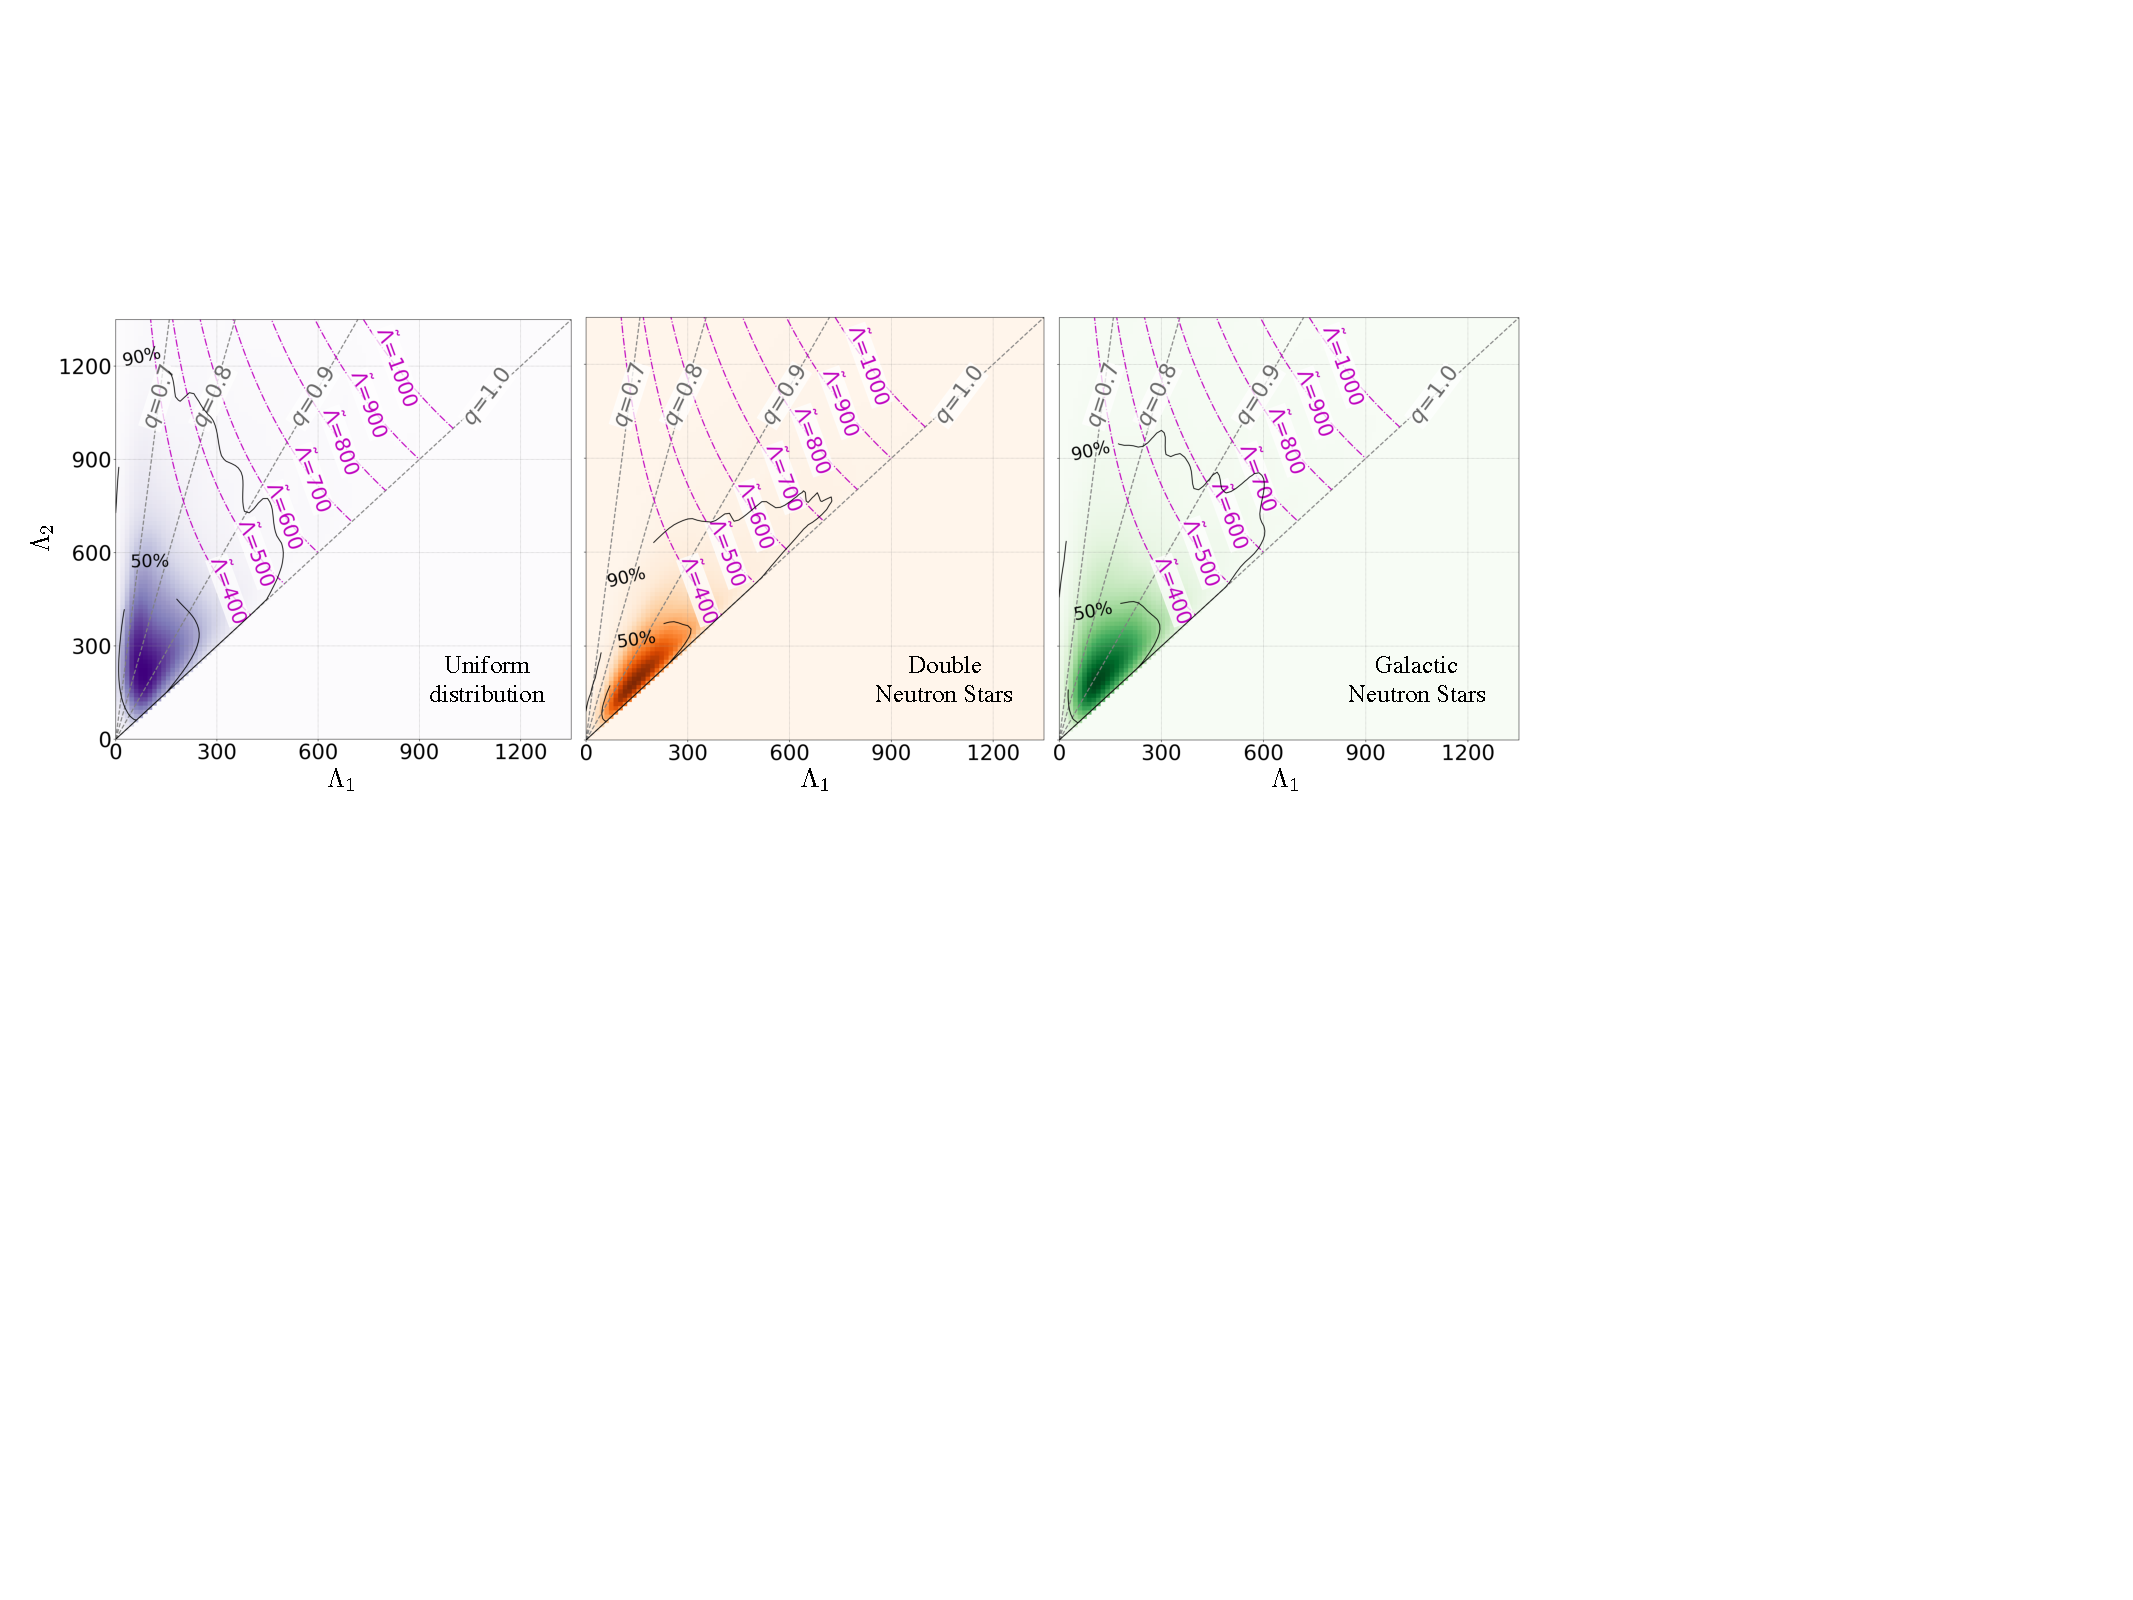
\includegraphics[width=\textwidth]{figures/common_eos/Lambda1_2_contours_no1D_w_q_moreiter.pdf}
  \caption{Posterior probability densities for $\Lambda_{1,2}$ with the common EOS constraint using uniform (left), double neutron stars (middle), and Galactic neutron stars (right) component mass priors. The 50$\%$ and 90$\%$ credible region contours are shown as solid curves. Overlaid are contours of $\tilde{\Lambda}$ (in magenta) and $q$ (in gray). The values of $\Lambda_1$ and $\Lambda_2$ forbidden by causality have been excluded from the posteriors.
\label{fig:lamb12_1abc}
%
%\vspace*{-0.3cm}%
}
\end{figure*}
\fi 

The choice of mass prior can have an impact on the recovery of the tidal deformability~\cite{Agathos:2015uaa}. To investigate this, we carry out our parameter estimation analyses using three different priors on the binary's component masses. First, we assume a uniform prior on each star's mass, with $m_{1,2} \sim U[1,2]\, M_\odot$. Then, we assume a Gaussian prior on the component masses $m_{1,2} \sim N(\mu = 1.33, \sigma = 0.09)\, M_\odot$, which is a fit to masses of neutron stars observed in  double neutron star systems~\cite{Ozel:2016oaf}. The third prior assumes that the component masses are drawn from a fit to the observed mass distributions of recycled and slow pulsars in the Galaxy with $m_1 \sim N(\mu = 1.54, \sigma = 0.23)\, M_\odot$ and $m_2 \sim N(\mu = 1.49, \sigma = 0.19)\, M_\odot$~\cite{Ozel:2016oaf}. We impose the constraint $m_1 \geq m_2$ which leads to $\Lambda_2 \geq \Lambda_1$. For all our analyses, the prior on the component spins is $\chi_{1,2} \sim U[-0.05,0.05]$, consistent with the expected spins of field binaries when they enter the LIGO-Virgo sensitive band~\cite{Brown:2012qf}.

\subsection{Technical details}\label{sec:pe_methods_ceos_tech_details}
To measure the source parameters for GW170817, we performed parameter estimation on the Advanced LIGO-Virgo data available at the LIGO Open Science Center \cite{Vallisneri:2014vxa,gw170817-losc}. 
Our analysis was performed with the \textit{PyCBC Inference} software \cite{Biwer:2018osg,alex_nitz_2018_1208115} and the parallel-tempered \textit{emcee} sampler \cite{emcee,vousden:2016} for sampling over the parameter space using Markov Chain Monte Carlo (MCMC) techniques \cite{mcmc}. 

The LOSC data files include a post-processing noise subtraction performed by the LIGO-Virgo Collaboration \cite{gw170817-losc,gw170817-noise}. The LOSC documentation states that these data have been truncated to remove tapering effects due to the cleaning process \cite{gw170817-losc}, however the LOSC data shows evidence of tapering after GPS time $1187008900$ in the LIGO Hanford detector. To avoid any contamination of our results we do not use any data after GPS time $1187008891$. The power spectral density (PSD) used to construct the likelihood was calculated using Welch's method \cite{1161901} with 16~second Hann-windowed segments (overlapped by 8~s) taken from GPS time $1187007048$ to $1187008680$. The PSD estimate is truncated to 8~s length in the time domain using the method described in Ref. \cite{Allen:2005fk}. The gravitational-wave data used in the likelihood is taken from the interval $1187008691$ to $1187008891$. 

Ref.~\cite{Abbott:2018wiz} found that choice of the low-frequency cutoff can have an effect on the measurement of the neutron star tidal deformability and used a different power spectral density estimation technique to that used in our analysis~\cite{Littenberg:2014oda}. We investigated the effect of changing our estimate of the power spectral density with the power spectral density released as supplemental materials to Ref.~\cite{Abbott:2018wiz}. We find that the change in parameter measurements is smaller than the statistical errors, and conclude that the choice of power spectral density estimation technique does not affect our results. To investigate the choice of low-frequency cutoff, we computed the measurabilities of the chirp mass $\mathcal{M}$, signal-to-noise ratio $\rho$, and binary deformability $\tilde{\Lambda}$ in the frequency range 10-2000~Hz. These are defined as the integrand as a function of frequency of the noise moment integrals $I_{\mathrm 10}$, $I_{\mathrm 0}$, and $I_{\mathrm -10}$ (see Ref.~\cite{Damour:2012yf}) and shown in Fig.~\ref{fig:measurability}. It can be seen that the signal-to-noise ratio is non-zero down to a frequency of $\sim$ 20~Hz for all the three detectors. While detector sensitivity at this frequency does not affect the measurability of $\tilde\Lambda$, it does affect the measurability of the chirp mass $\mathcal{M}$. We repeated our analyses at 25~Hz, 23~Hz, and 20~Hz, and found an improvement in the $\mathcal{M}$ measurement when extending until the low-frequency cutoff was 20~Hz. Consequently, we evaluated the likelihood from a low-frequency cutoff of 20~Hz to the Nyquist frequency of 2048~Hz. The improved measurement of $\mathcal{M}$ eliminates regions of higher $\tilde{\Lambda}$ values from the posterior probability densities, and hence better constrains the measurement of this parameter, as shown in Fig~\ref{fig:posterior_overlap}.

\begin{figure}[t]
  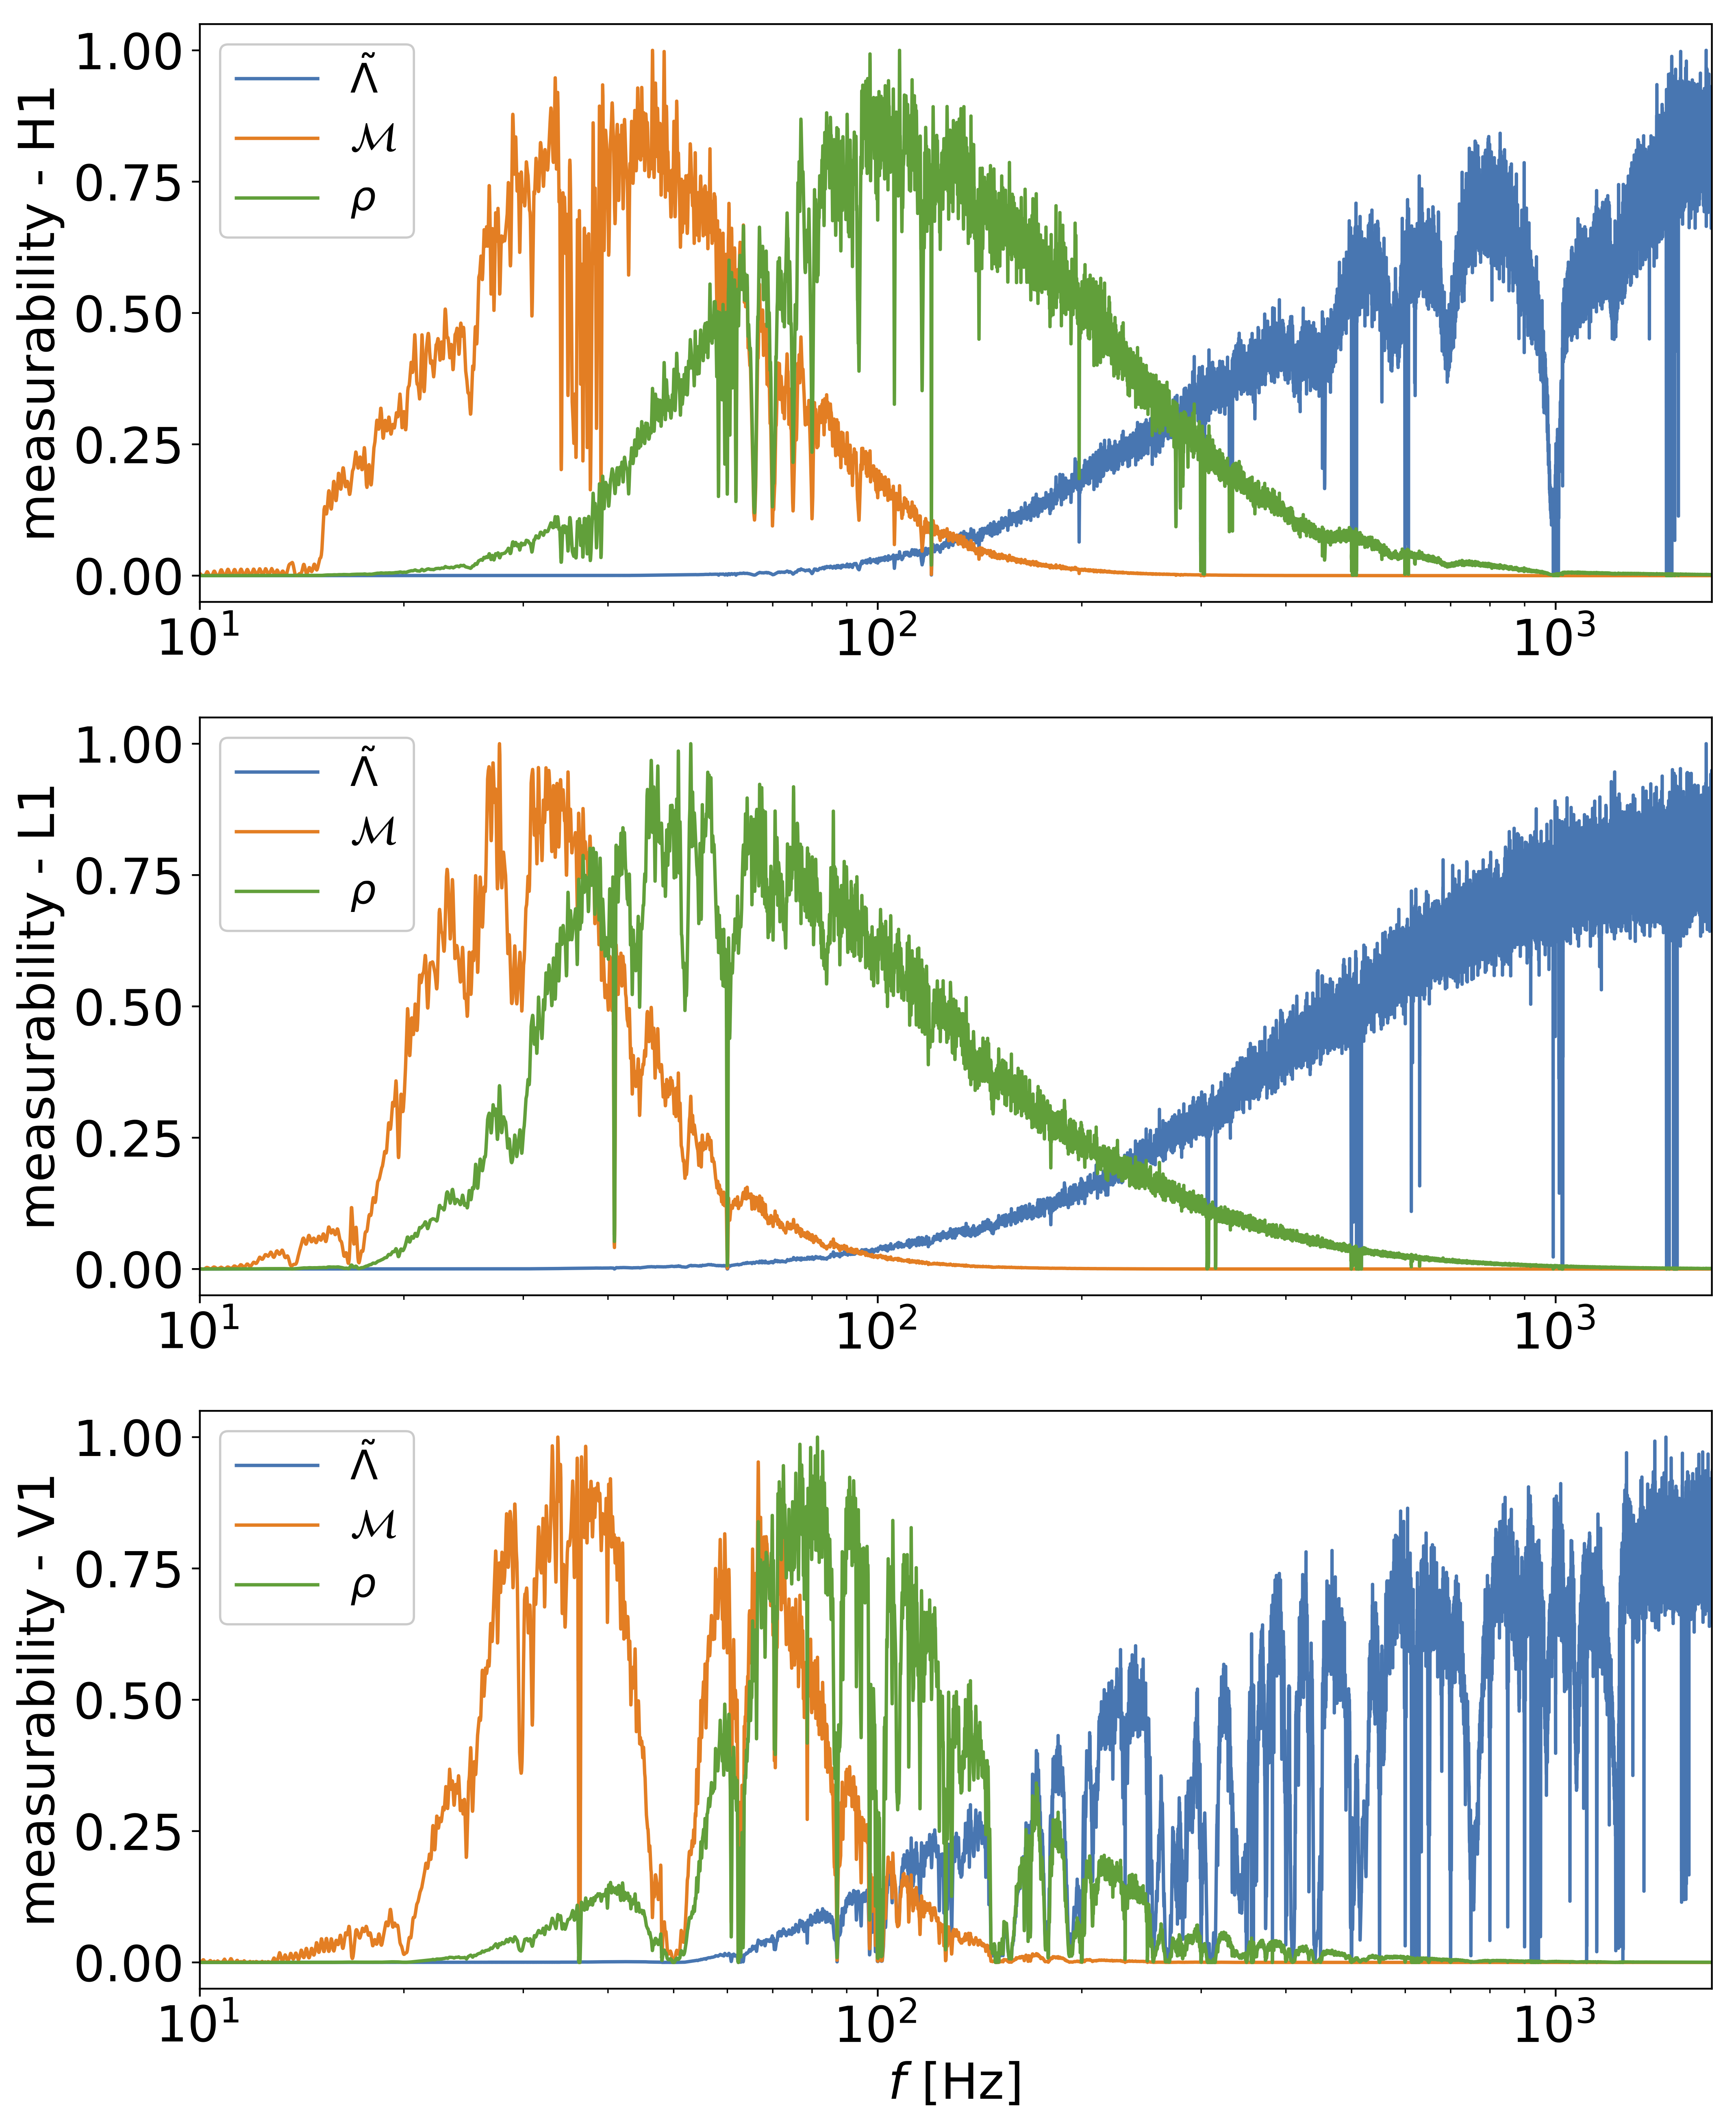
\includegraphics[width=14cm]{figures/common_eos/measurability_plots.png}
  \caption{Measurability~\cite{Damour:2012yf} of the chirp mass $\mathcal{M}$, SNR $\rho$ and binary deformability $\tilde{\Lambda}$ in the frequency range 10 Hz - 2000 Hz. Each detector's parameter measurability is scaled to the maximum frequency to show the relative accumulation of measurement over the detector's frequency band. Note that between detectors, L1 is more sensitive than H1, which is more sensitive than V1. Measurability of chirp mass is accumulated primarily at low frequencies, whereas measurability of tidal deformability is accumulated at higher frequencies. We extend computation of the likelihood down to $20$~Hz where the measured signal-to-noise ratio (the logarthim of the likelihood) drops to zero in all three detectors. 
  \label{fig:measurability}}
\end{figure}

The templates for the waveforms used in our parameter estimation analysis are generated using the restricted TaylorF2 waveform model, a Fourier domain waveform model generated using stationary phase approximation. We use the implementation from the LIGO Algorithm Library (LAL)~\cite{lal} accurate to 3.5 post-Newtonian (pN) order in orbital phase \cite{Buonanno:2009zt}, 2.0 pN order in spin-spin, quadrupole-monopole and self-spin interactions\cite{Arun:2008kb,Mikoczi:2005dn}, and 3.5 pN order in spin-orbit interactions \cite{Bohe:2013cla}. The tidal corrections enter at the 5 pN and 6 pN orders~\cite{Vines:2011ud}. The waveforms are terminated at twice the orbital frequency of a test particle at the innermost stable circular orbit of a Schwarzschild black hole of mass $M = m_1 + m_2$, where $m_{1,2}$ are the masses of the binary's component stars. The TaylorF2 model assumes that the spins of the neutron stars are aligned with the orbital angular momentum. Binary neutron stars formed in the field are expected to have small spins, and precession of the binary's orbital plane is not significant~\cite{Brown:2012qf}. 

We fix the sky location of the binary to the right ascension RA =  $197.450374^\circ$ and declination Dec = $-23.381495^\circ$ \cite{Soares-Santos:2017lru} for all of our runs. We also fix the luminosity distance of NGC\,4993 $d_L = 40.7$~Mpc~\cite{Cantiello:2018ffy}. The small error in the known distance of NGC\,4993 produces errors that are much smaller than the errors in measuring the tidal deformability. We have checked that including the uncertainty in the distance error does not affect our conclusions of the tidal deformabilities or radius. The MCMC computes the marginalized posterior probabilities for the remaining source parameters: chirp mass $\mathcal{M}$, mass ratio $q$, the component (aligned) spins $\chi_{1,2} = c J_{1,2}/G m_{1,2}^2$, component tidal deformabilities $\Lambda_{1,2}$, polarization angle $\psi$, inclination angle $\iota$, coalescence phase $\phi_c$, and coalescence time $t_c$. When generating the waveform in the MCMC, each $m_{1, 2}$ draw follows the constraint $m_1 \geq m_2$, and the masses are transformed to the detector frame chirp mass $\mathcal{M}^\mathrm{det}$ and $q$ with a restriction $1.1876 \le \mathcal{M}^\mathrm{det} \le 1.2076$.

\begin{figure}[b]
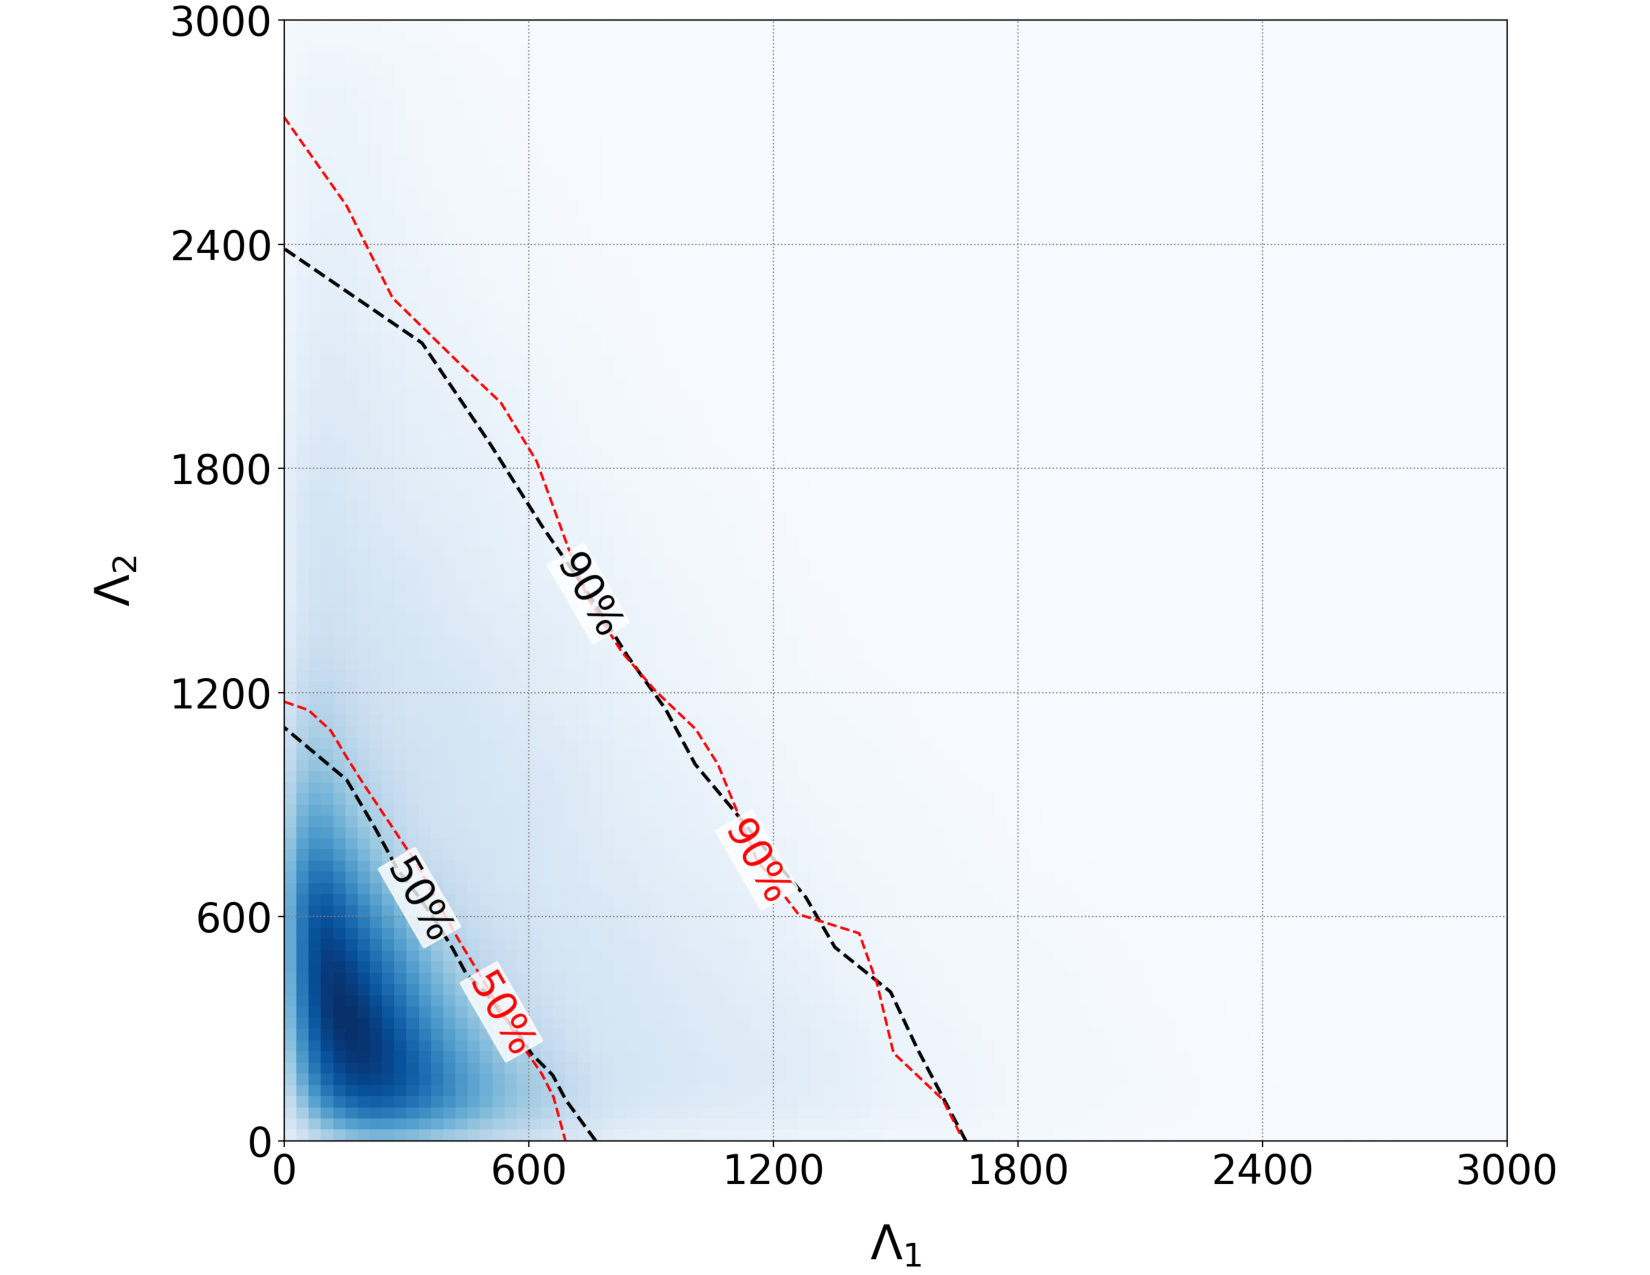
\includegraphics[width=\textwidth]{figures/common_eos/lambda1_2_3x_ul.pdf}
\caption{Posterior probability density function for $\Lambda_1$, $\Lambda_2$ from unconstrained $\Lambda_{1,2} \sim U[0, 3000]$, $m_{1,2} \sim U[1, 2]$ M$_\odot$, $1.1876 \leq \mathcal{M} \leq 1.2076$, $m_1 \geq m_2$, 30~Hz low-frequency cutoff analysis. The black dotted lines show 50\% and 90\% upper limits from our analysis. The red dotted lines show 50\% and 90\% upper limits from the LIGO-Virgo analysis \cite{TheLIGOScientific:2017qsa}. } 
\label{fig:lv_compare}
\end{figure}

For direct comparison with the results of Ref.~\cite{TheLIGOScientific:2017qsa}, Fig~\ref{fig:lv_compare} shows the posterior probability densities for $\Lambda_{1,2}$ for an MCMC using a $30$~Hz low-frequency cutoff for the uniform component mass prior $m_{1,2} \sim U[1,2]\, M_\odot$, and assuming that the priors on $\Lambda_{1,2}$ are completely uncorrelated ($\Lambda_{1,2} \sim U[0,3000]$). No cut is placed on $\tilde\Lambda$ in this analysis. We have digitized the 50\% and 90\% contours from Fig.~5 of Ref.~\cite{TheLIGOScientific:2017qsa} and compared them to 50\% and 90\% upper limit contours for our result computed using a radial binning to enclose 50\% and 90\% of the posterior probability starting from $\Lambda_1 = \Lambda_2 = 0$. The 90\% contours agree well, with a slight difference in the 50\% contours. Given the accuracy of measuring the tidal deformability, this difference can 
be attributed to small differences in the technical aspects of our analysis compared to that of Ref.~\cite{TheLIGOScientific:2017qsa}. We note that the 90\% confidence contour of Fig.~5 in Ref.~\cite{TheLIGOScientific:2017qsa} with $\Lambda_1=\Lambda_2$, passes through $\tilde\Lambda \approx 1100$. If we impose $\Lambda_1=q^6 \Lambda_2$, then this contour continues to follow $\tilde\Lambda \approx 1100$ for $q \leq 1$. We interpret the difference between this result and the result of Table~I of Ref.~\cite{TheLIGOScientific:2017qsa} $\tilde\Lambda \le 800$ (90\% confidence) as being due to a different choice of prior on $\tilde\Lambda$ (one non-uniform and one uniform).

\begin{figure}[t]
\centering
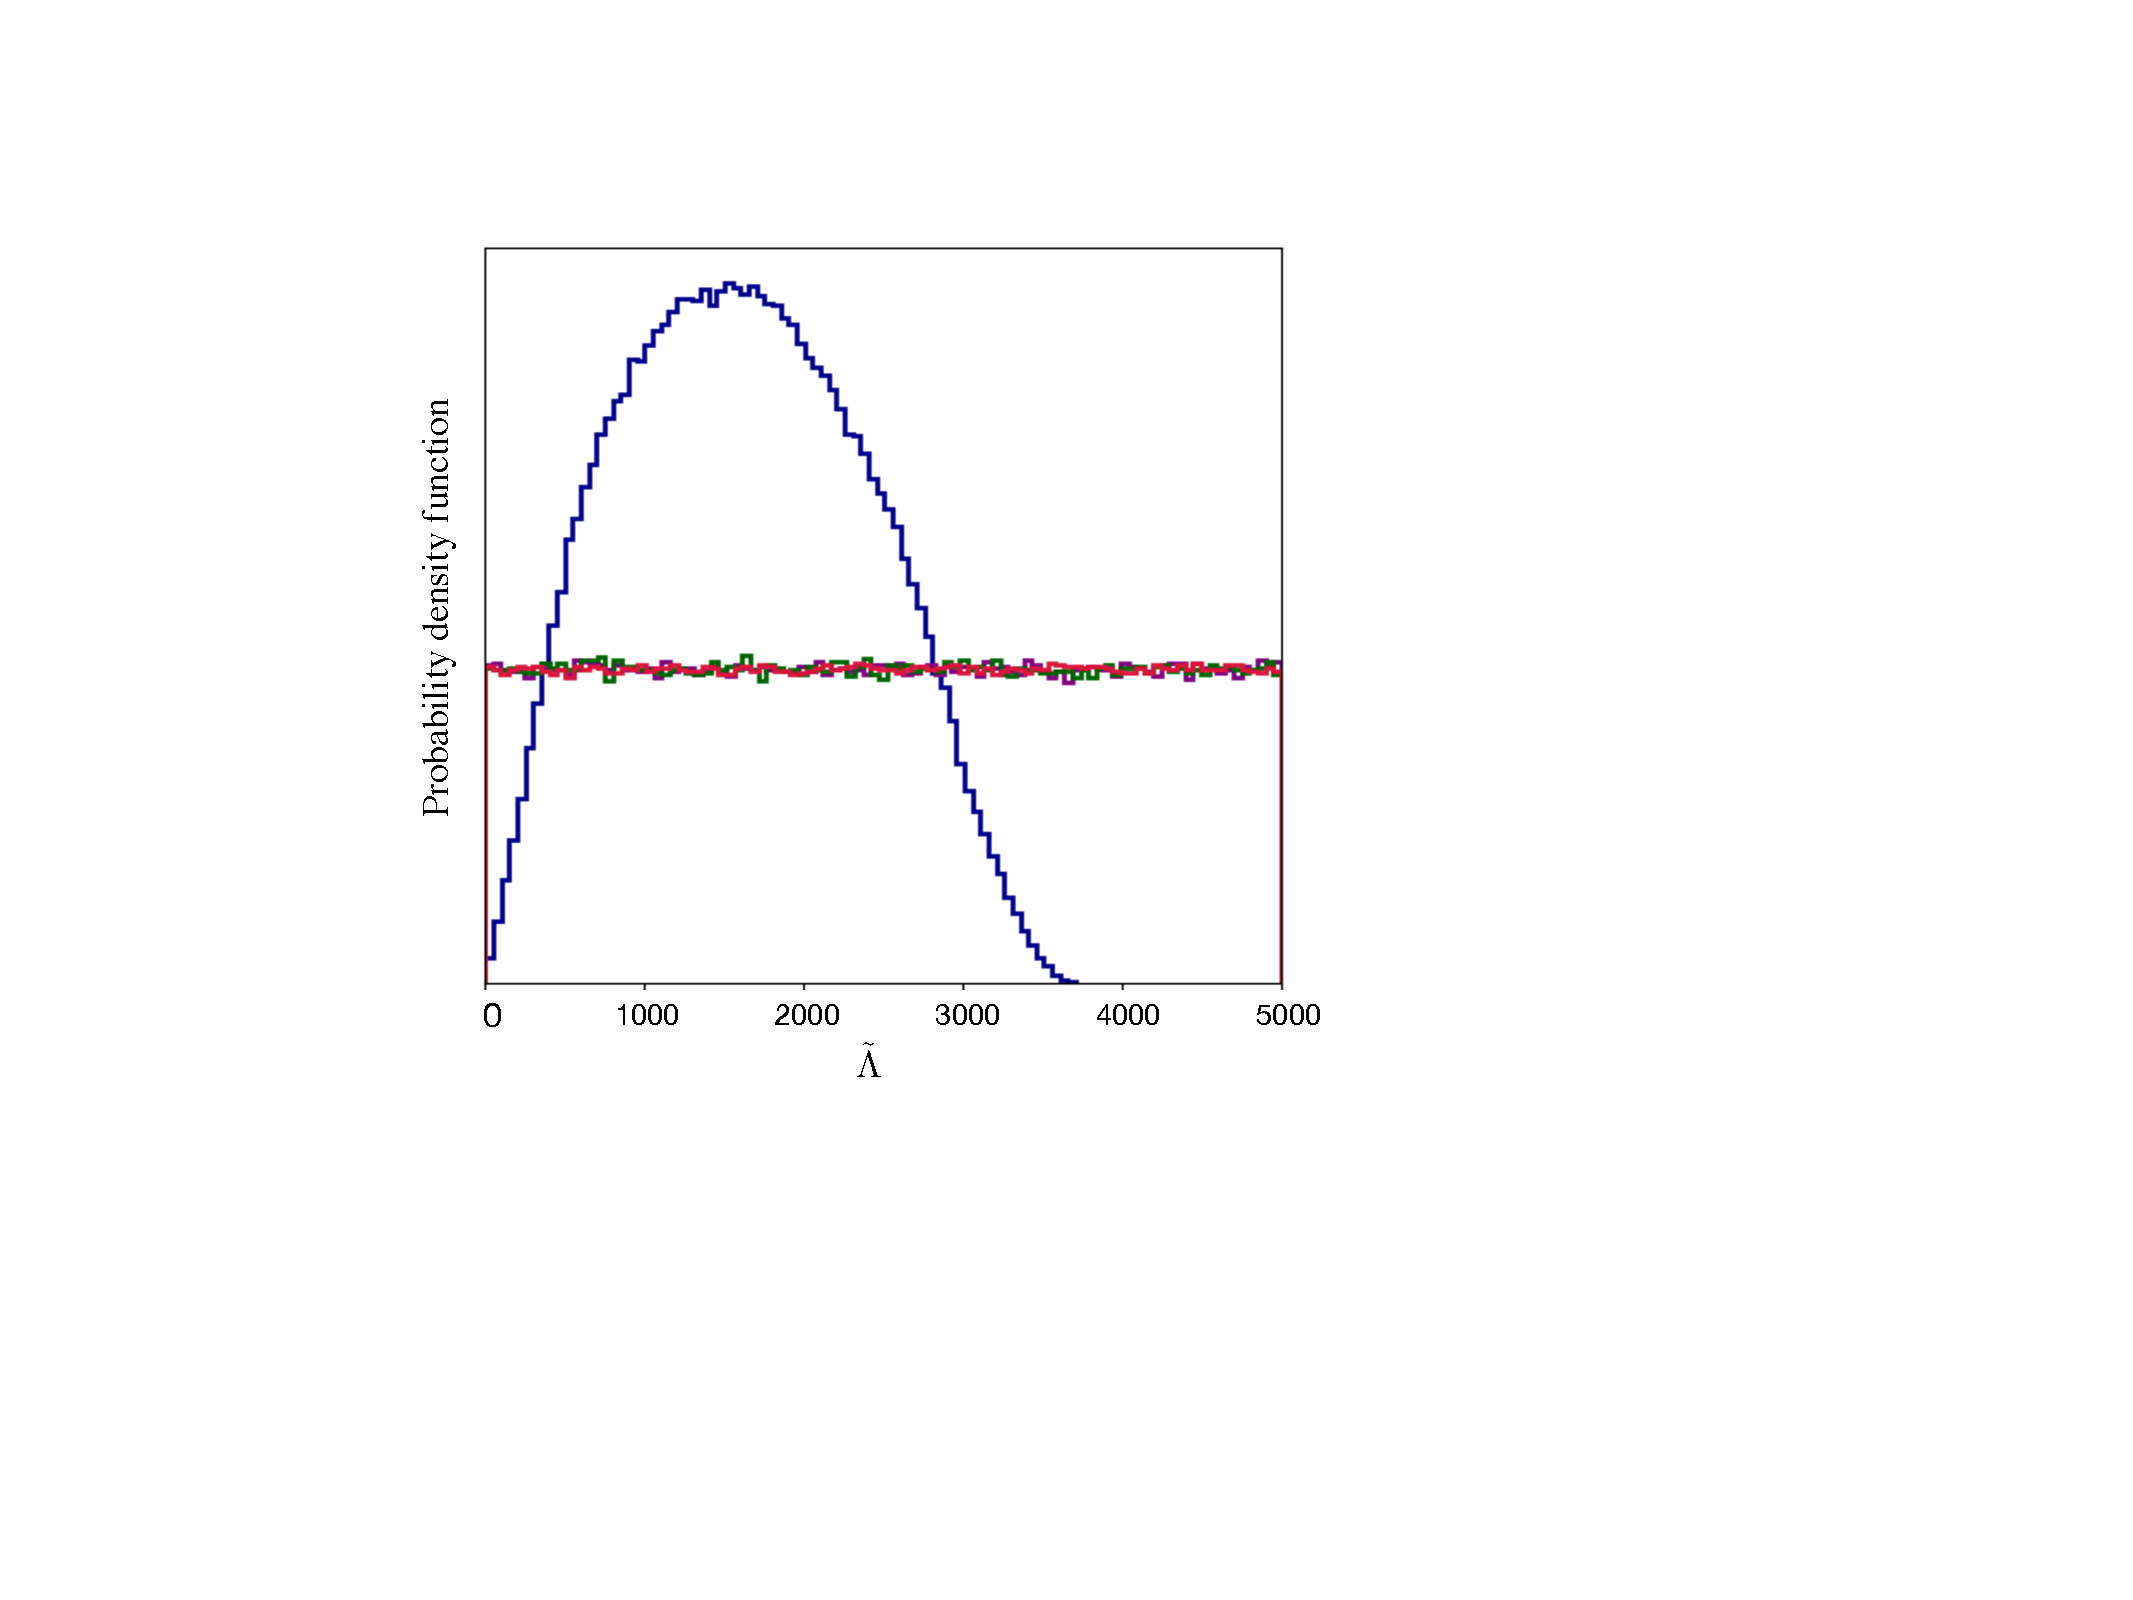
\includegraphics[width=\textwidth,height=7cm,width=8.5cm]{figures/common_eos/prior_lambdatilde.pdf}
\caption{Comparison of the prior probability distributions on $\tilde\Lambda$ for the three mass priors imposing the common EOS constraint: uniform (purple), double neutron stars (red), galactic neutron stars (green) with a prior in $\Lambda_{1,2} \sim U[0, 3000]$ and $m_{1,2} \sim U[1, 2] M_\odot$, $m_1 \geq m_2$ without the common EOS constraint (blue). The priors in the common EOS analysis are uniform across the region of interest.} 
\label{fig:lambda_priors}
\end{figure}


Our common equation of state constraint is implemented in the MCMC by drawing a variable $\Lambda_s \sim U[0,5000]$, drawing the component masses from their respective priors and computing
\begin{equation}
\Lambda_1=q^3\Lambda_s,\qquad\Lambda_2=q^{-3}\Lambda_s,
\label{eq:lambdas_supp}\end{equation}
with draws that have $\tilde\Lambda > 5000$ discarded. This produces a prior that is uniform in $\tilde\Lambda$ between 0 and 5000, as shown in Fig.~\ref{fig:lambda_priors} for all of our three mass priors discussed in Section \ref{sec:pe_methods_ceos_summ}. For comparison, we also show the prior on $\tilde\Lambda$ computed assuming independent $\Lambda_{1,2} \sim U[0,3000]$ and the component mass prior $m_{1,2}\sim U[1,2]\,M_\odot$. It can be seen that this prior vanishes as $\tilde\Lambda \rightarrow 0$ and so can bias the posterior at low values of   $\tilde\Lambda$. In addition to the physical requirement of a common EOS constraint, the prior used in the common EOS analysis is uniform as $\tilde\Lambda \rightarrow 0$, allowing us to fully explore likelihoods in this region, and set lower bounds on our credible intervals.

%SOUMI: Inserted from Supp Materials
\section{The common neutron star radius}\label{sec:ceos_radius}

To validate the relationship
\begin{equation}
\tilde{\Lambda}=a^\prime\left(\frac{\hat{R}c^2}{G{\cal M}}\right)^6,
\label{eq:lambda_t2_supp}\end{equation}
where $a^\prime=0.0042\pm0.0004$, we perform Tolman-Oppenheimer-Volkoff (TOV) integrations~\cite{Oppenheimer:1939ne} as described in Section \ref{sec:ceos_constraint}.
\begin{figure}[b]
  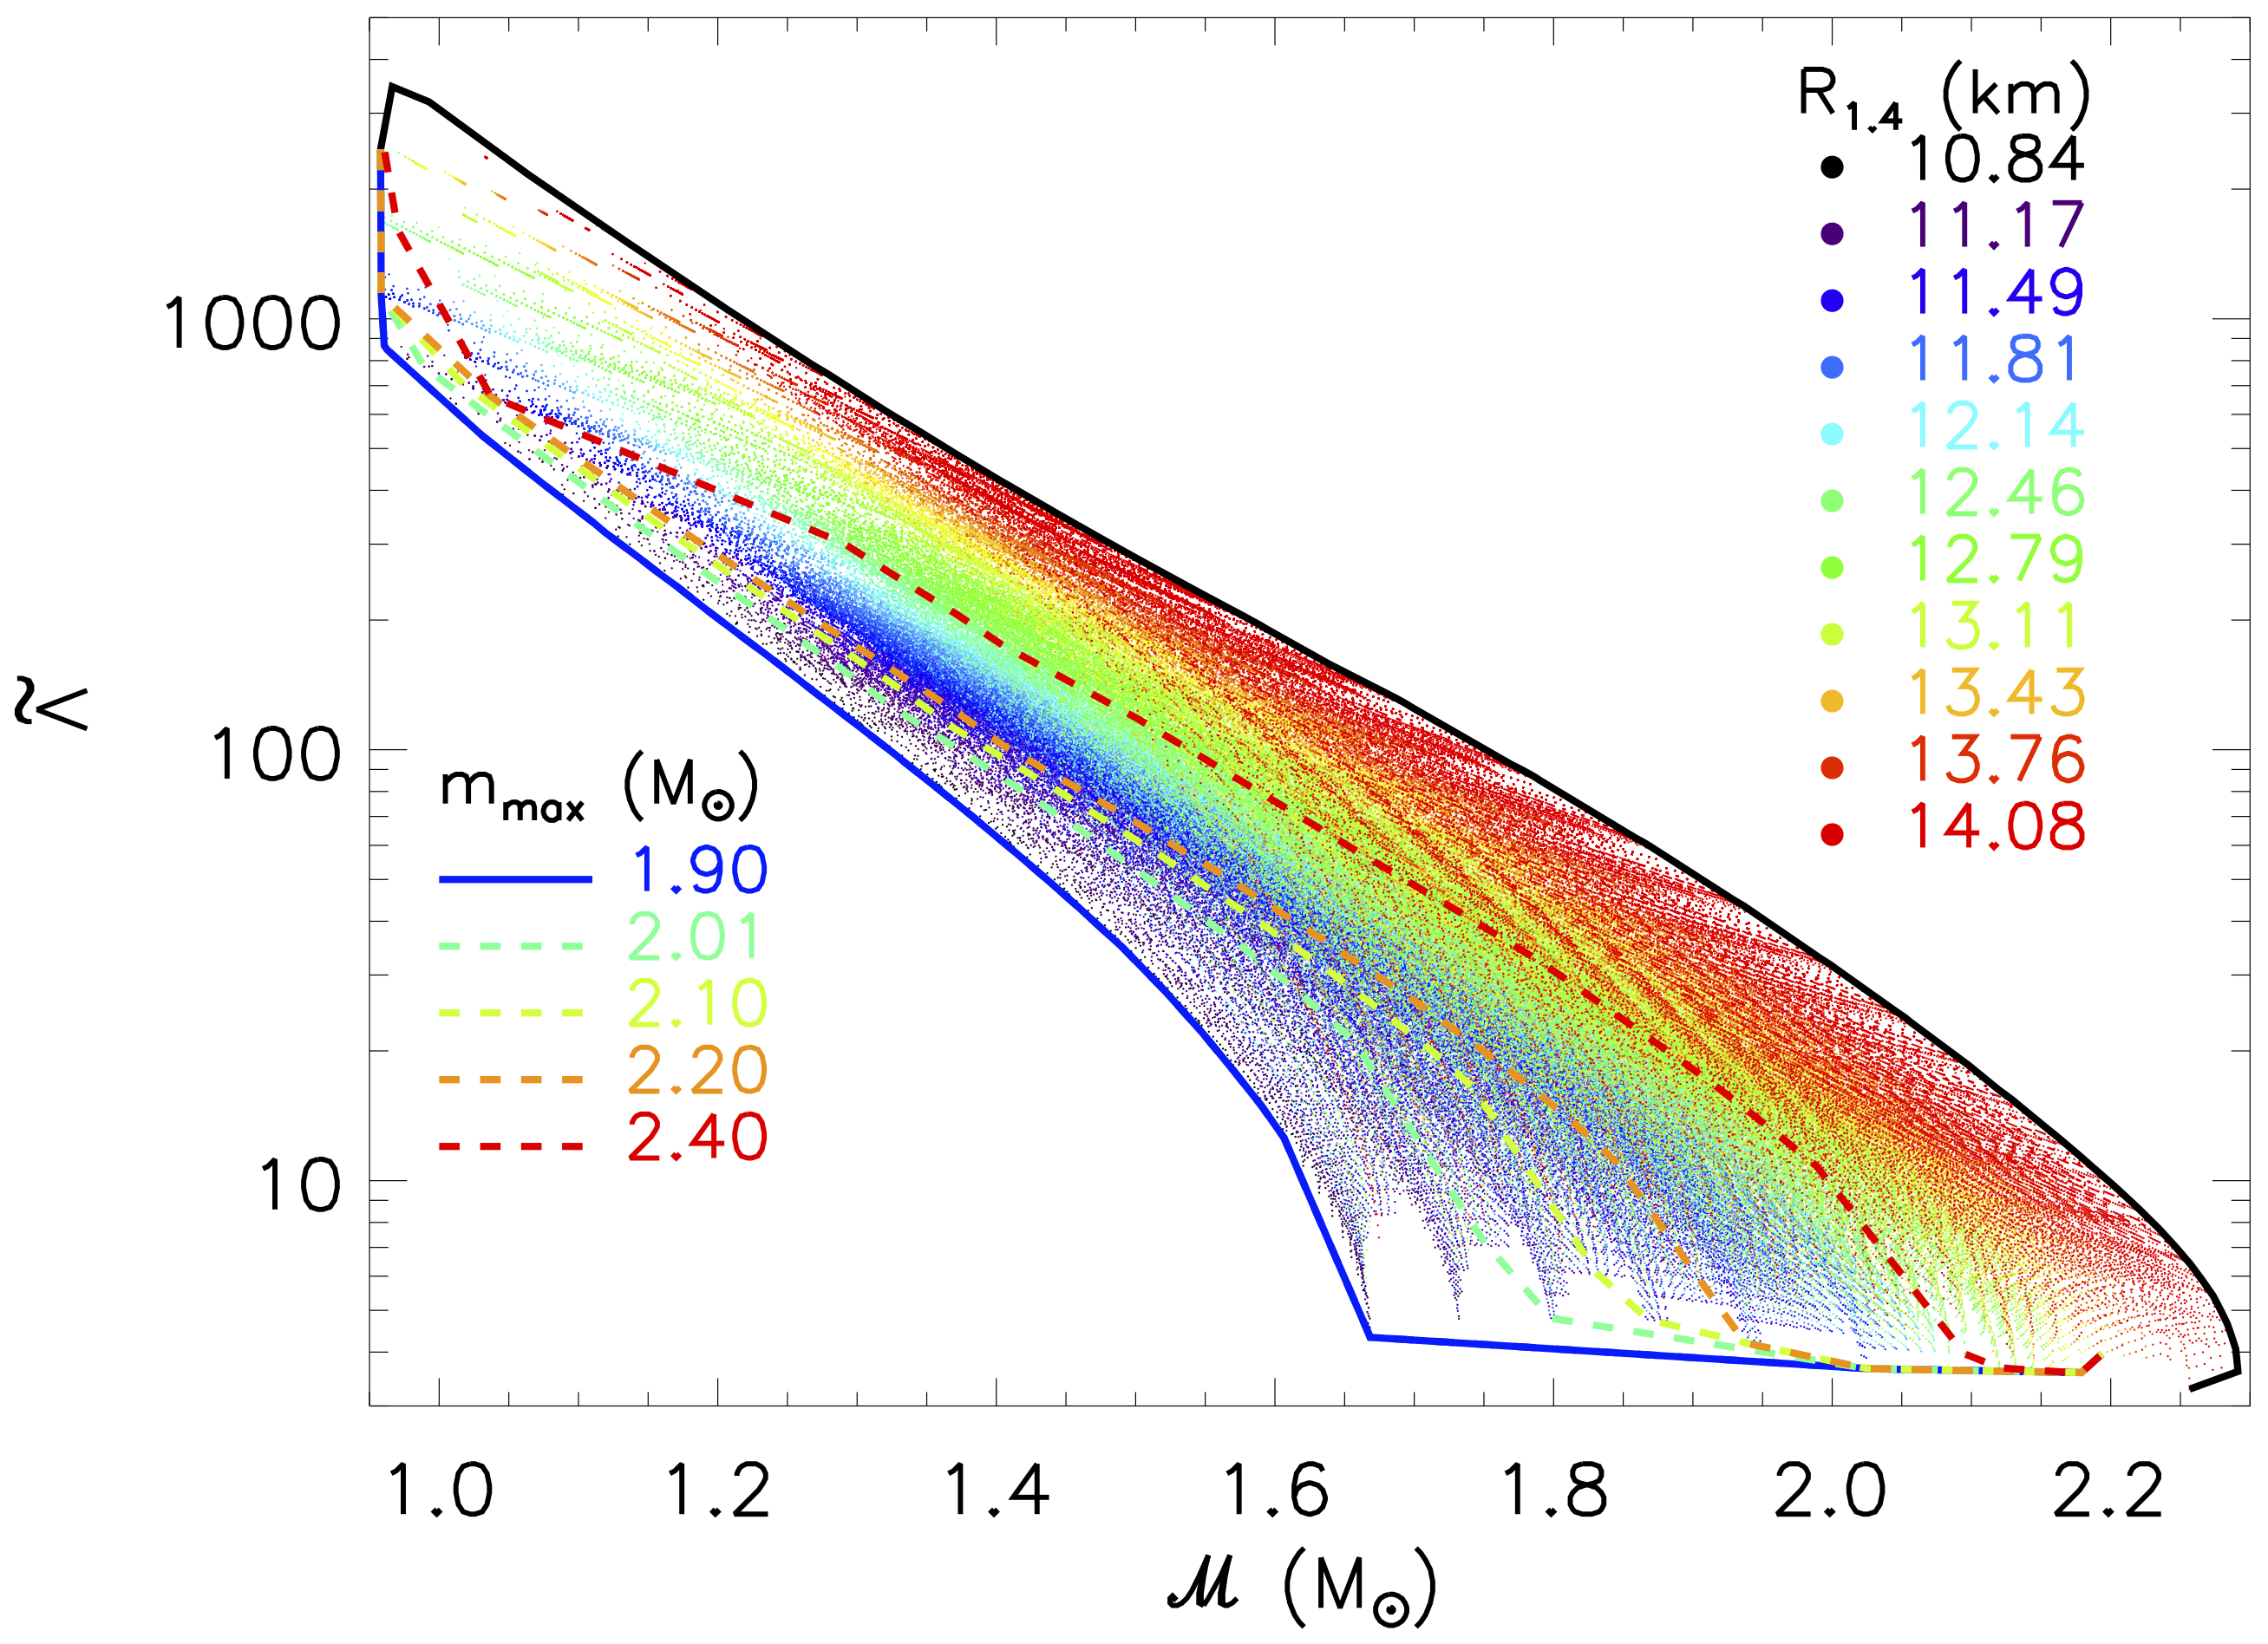
\includegraphics[width=\columnwidth]{figures/common_eos/lambdatilde_mchirp.png}
  \caption{The dimensionless binary tidal deformability $\tilde \Lambda$ as a function of chirp mass $\cal{M}$ for piecewise polytropes with parameters bounded by causality, neutron matter studies and nuclear experiments. Various binary mass combinations with each equation of state result in many points which are color-coded according to that equation of state's value of $R_{1.4}$.  The values of $\tilde\Lambda(\cal{M})$ are bounded according to the assumed value of the maximum neutron star mass, $m_\mathrm{max}$. \label{fig:lambar-mass}}
\end{figure}

The relationship between $\tilde\Lambda$, chirp mass ${\cal M}$ and the common radius $\hat R$ closely resembles the relation between $\Lambda$, the neutron star mass $m$ and radius $R$. We confirm this using piecewise polytropes as shown in Fig.~\ref{fig:lambar-mass}, which was prepared using the results computed to create Fig.~1 in Section \ref{sec:ceos_constraint}. A single mass-radius curve is generated for each equation of state containing $N$ masses between $1M_\odot$ and $m_\mathrm{max}$ for that EOS. $N(N-1)$ values of $\tilde\Lambda$ and $\cal{M}$ are then computed for all the unique combinations of $m_1$ and $m_2$ from these $N$ masses. The resulting points are plotted in Fig.~\ref{fig:lambar-mass}, and are color-coded by that equation of state's value of $R_{1.4}$. The process is repeated for all combinations of the parameters controlling the piecewise polytropic EOS described in \cite{Lattimer:2015nhk}. For the entries bounded by $0.9 M_\odot\le~{\cal M} \le~1.3M_\odot$, an interval including GW170817, Eq. (\ref{eq:lambda_t2_supp}) is determined by finding the upper and lower bounds of $a^\prime=\tilde\Lambda[G{\cal M}/(R_{1.4}c^2)]^6$.

\begin{figure}[t]
  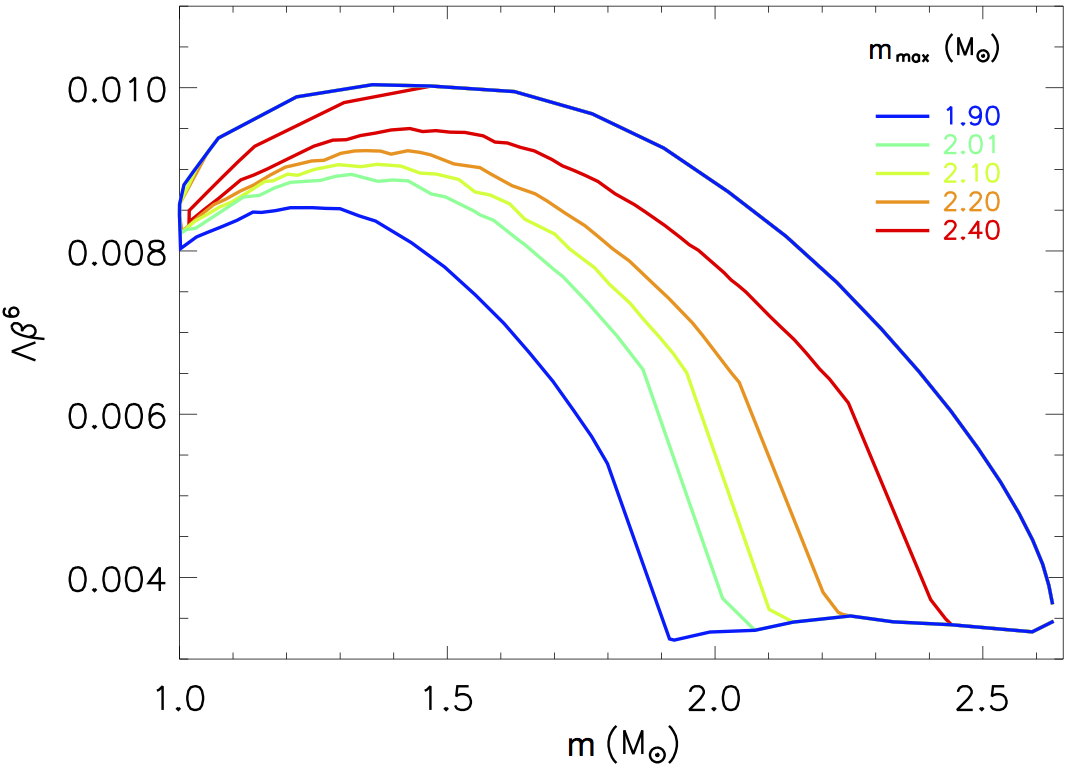
\includegraphics[width=\textwidth]{figures/common_eos/lamb6.png}
  \caption{$\Lambda \beta^{6}$ as a function of neutron star mass $m$ for physically realistic polytropes. The curves show lower bounds to $\Lambda$ for a given mass $m$ for different assumed lower limits to the neutron star maximum mass, $m_\mathrm{max}$. The curves are colored by $m_\mathrm{max}$. All values of $m_\mathrm{max}$ produce the same upper bound. \label{fig:lam-beta6}}
\end{figure}

The numerical results also confirmed our value for $a^\prime$. This is valid for values of $\mathcal{M} < 1.3 M_\odot$, which is relevant not only for GW170817 but also for all known double neutron star binaries, which are clustered in the narrow range $1.09M_\odot<{\cal M}<1.25M_\odot$ \cite{Tauris:2017omb,Ozel:2016oaf,Lattimer:2012nd}. The robustness of $\tilde{\Lambda}\propto\beta^{-6}$ confirms that the assumption $R_1=R_2$ is a valid proposition. To justify the degree of correlation in the $\Lambda~\simeq a\beta^{-6}$ that we established in Section \ref{sec:ceos_constraint}, we show in Fig.~\ref{fig:lam-beta6} the dependence of $\Lambda \beta^{6}$ on $m$. The variation of $\Lambda \beta^{6}$ is negligible in the mass range relevant for GW170817, $1.1 < m < 1.6 M_\odot$, thus confirming the validity of the $\Lambda~\simeq a\beta^{-6}$ relation for GW170817.

\section{Causal constraints on the tidal deformation}

The posterior probability distribution that we observe for the star's tidal deformability includes regions forbidden by causality~\cite{Zhao:2018nyf}. In our results for $\Lambda$ and (and hence $\hat{R}$), we apply the causal lower limit constraint on the tidal deformability $\Lambda$ as a function of mass $m$. We implement this constraint using the following relation, which is valid for $0.4 < m/m_{max} < 0.95$,
\begin{equation}
\begin{split}
\ln\Lambda_{\mathrm min} = 13.42 - 23.01\left(\frac{m}{m_{\mathrm max}}\right) \\
+ 20.53 \left(\frac{m}{m_{\mathrm max}}\right)^2 \\
- 9.599\left(\frac{m}{m_{\mathrm max}}\right)^3.
\end{split}
\end{equation}
Here, we use $m_{\mathrm max} = 2 M_\odot$. Note that $m_{\mathrm max} > 2$, would increase the lower limit for $\Lambda(m)$, so $m_{\mathrm max}=2$ is a conservative choice~\cite{Zhao:2018nyf}.


\section{Results}

%SOUMI commented for thesis:We perform parameter estimation for each mass prior with and without the common EOS constraint and calculate the Bayes factor---the ratio of the evidences $p(\vec{d}(t)|H)$---between the common EOS constrained and unconstrained analyses. We find Bayes factors $\mathcal{B}$ of 369, 125, and 612 for the three mass priors, respectively, indicating that the data strongly favor the common EOS constraint in all cases. 
%The full posterior probability densities of the parameters $p(\vec{\theta}|\vec{d}(t),H)$ for the common EOS runs are shown in the Section \ref{sec:pe_methods_ceos_tech_details} %Supplemental Material~\cite{supp} 
%and are available for download at Ref.~\cite{gw170817commoneos}. 
Figure \ref{fig:lamb12_1abc} shows the posterior probability densities for $\Lambda_1$ and $\Lambda_2$ with 90\% and 50\% credible region contours, for the common EOS runs. Overlaid are $q$ contours and $\tilde{\Lambda}$ contours obtained from Eq.~(\ref{eq:lambda_t0}), $\Lambda~\simeq a\beta^{-6}$, and $R_1 \simeq R_2 \simeq \large \hat R$ as
\begin{equation}
\Lambda_1(\tilde{\Lambda},q)={\frac{13}{16}}\tilde{\Lambda}{\frac{q^2(1+q)^4}{12q^2-11q+12}},
\label{eq:l1l2}\quad \Lambda_2(\tilde{\Lambda},q) = q^{-6} \Lambda_1 .\end{equation}
Because of our constraint $\Lambda_2 \geq \Lambda_1$, our credible contours are confined to the region where $q \leq 1$. One can easily demonstrate that $\Lambda_2 \geq \Lambda_1$ is valid unless $(c^2/G)dR/dm > 1$, which is impossible for realistic equations of state. For the entire set of piecewise polytropes satisfying $m_\mathrm{max}>2M_\odot$ we considered, $(c^2/G)dR/dm$ never exceeded 0.26. Even if a first order phase transition appeared in stars with masses between $m_2$ and $m_1$, it would necessarily be true that $dR/dm < 0$ across the transition. Because of the $q$ dependence of $\Lambda_1$, $\Lambda_2$, the credible region enclosed by the contours broadens from the double neutron star (most restricted), to the pulsar, to the uniform mass (least restricted) priors. However, the upper bound of the credible region is robust.

\begin{figure*}[t]
  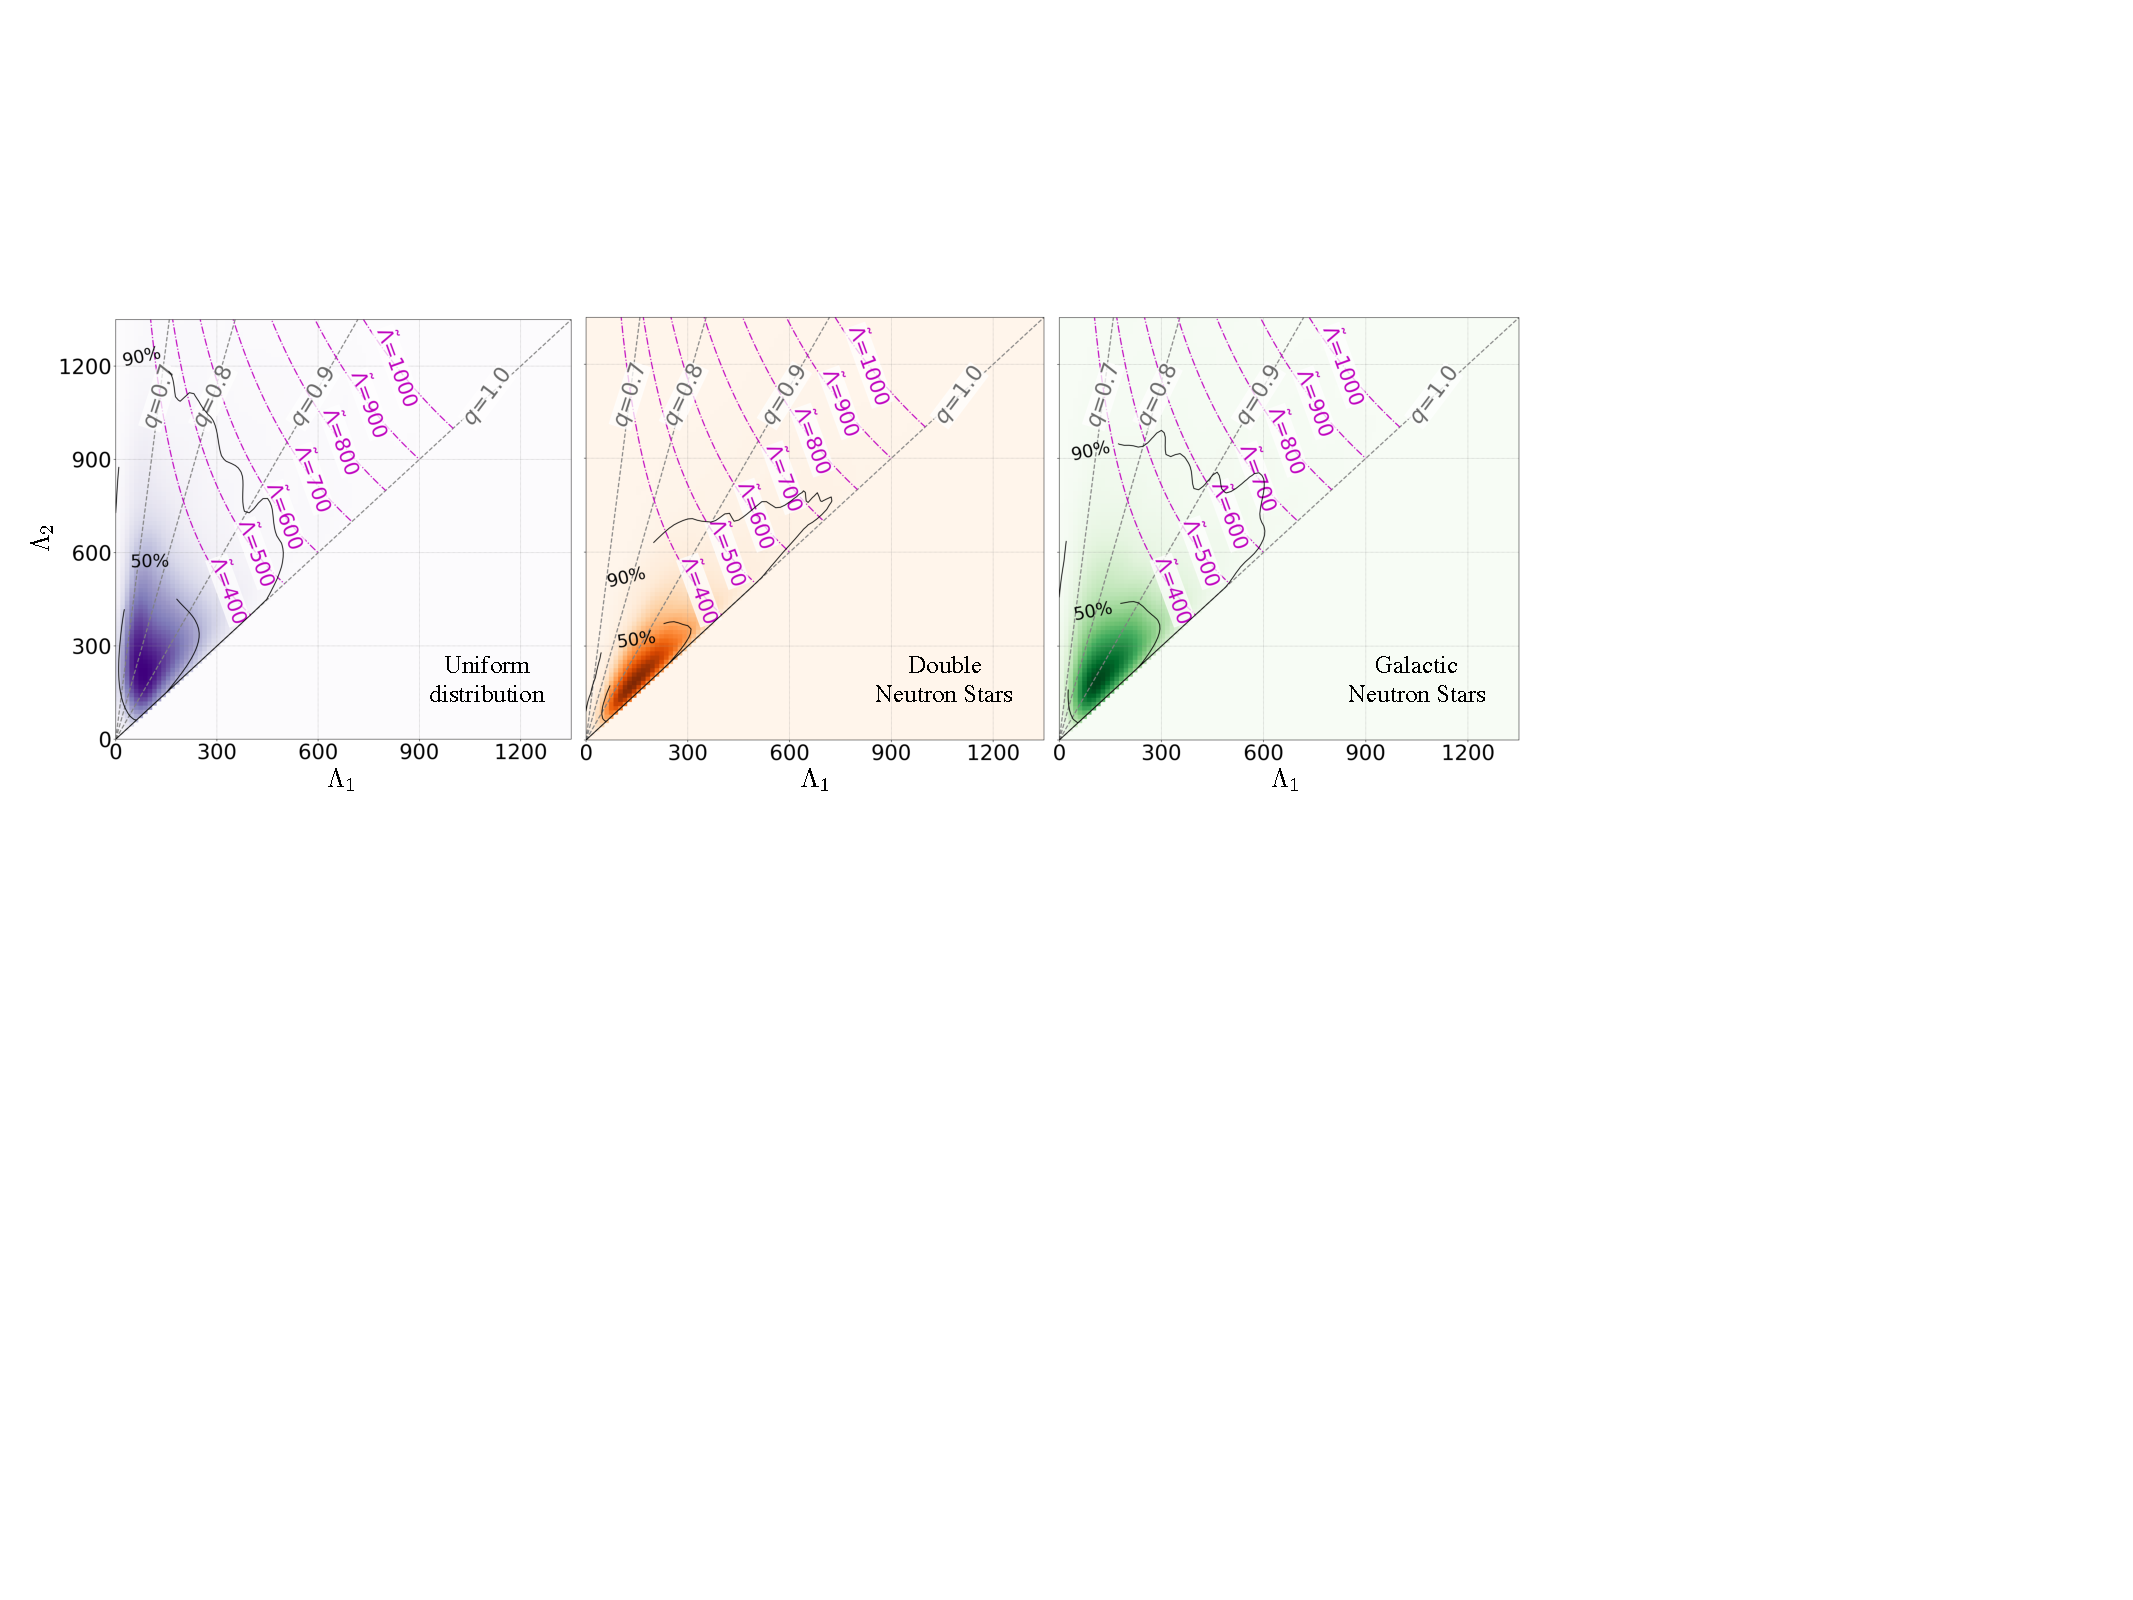
\includegraphics[width=\textwidth]{figures/common_eos/Lambda1_2_contours_no1D_w_q_moreiter.pdf}
  \caption{Posterior probability densities for $\Lambda_{1,2}$ with the common EOS constraint using uniform (left), double neutron stars (middle), and Galactic neutron stars (right) component mass priors. The 50$\%$ and 90$\%$ credible region contours are shown as solid curves. Overlaid are contours of $\tilde{\Lambda}$ (in magenta) and $q$ (in gray). The values of $\Lambda_1$ and $\Lambda_2$ forbidden by causality have been excluded from the posteriors.
\label{fig:lamb12_1abc}
%
%\vspace*{-0.3cm}%
}
\end{figure*}

We find $\tilde{\Lambda}=
205^{+415}_{-167}$ for the uniform component mass prior, $\tilde{\Lambda}=234^{+452}_{-180}$ for the prior informed by double neutron star binaries in the Galaxy, and $\tilde{\Lambda}=218^{+445}_{-173}$ for the prior informed by all Galactic neutron star masses (errors represent 90\% credible intervals). Our measurement of $\tilde{\Lambda}$ appears to be robust to the choice of component mass prior, within the (relatively large) statistical errors on its measurement. The Bayes factors comparing the evidence from the three mass priors are of order unity, so we cannot claim any preference between the mass priors.

The 90\% credible intervals on $\tilde{\Lambda}$ obtained from the gravitational-wave observations include regions forbidden by causality. Applying a constraint to our posteriors for the causal lower limit of $\Lambda$ as a function of $m$~\cite{Zhao:2018nyf}, we obtain $\tilde{\Lambda}=
222^{+420}_{-138}$ for the uniform component mass prior, $\tilde{\Lambda}=245^{+453}_{-151}$ for the prior informed by double neutron star binaries in the Galaxy, and $\tilde{\Lambda}=233^{+448}_{-144}$ for the prior informed by all Galactic neutron star masses (errors represent 90\% credible intervals). Using Eq.~(\ref{eq:rhat}), we map our $\cal{M}$ posteriors and $\tilde{\Lambda}$ posteriors (with the causal lower limit applied) to $\hat{R} \simeq R_{1.4}$ posteriors, allowing us to estimate the common radius of the neutron stars for GW170817 for each mass prior. Figure~\ref{fig:radius_lambda} shows the posterior probability distribution for the binary tidal deformation $\tilde\Lambda$ and the common radius $\hat{R}$ of the neutron stars in the binary. Our results suggest a radius $\hat R = 10.7^{+2.1}_{-1.6} \pm 0.2$ km (90\% credible interval, statistical and systematic errors) for the uniform mass prior,  $\hat R = 10.9^{+2.1}_{-1.6} \pm 0.2$ km for double neutron star mass prior, and $\hat R = 10.8^{+2.1}_{-1.6} \pm 0.2$ km for the prior based on all neutron star masses.

%SOUMI commented for thesis: For the uniform mass prior, we computed the Bayes factor comparing a model with a prior $\Lambda_s \sim U[0,5000]$ to a model with a prior $\Lambda_s \sim U[0,100]$. We find $\log_{10}(\mathcal{B}) \sim 1$, suggesting that the data favors a model that includes measurement of tidal deformability $\tilde\Lambda \gtrsim 100$. However, the evidences were calculated using thermodynamic integration of the MCMC chains~\cite{emcee}. We will investigate model selection using, e.g., nested sampling \cite{skilling2006} in a future work.

%SOUMI: Added from Supp Materials Results section
Fig.~\ref{fig:posterior_overlap} shows the full posterior probability densities for the parameters of interest in our study: the source frame chirp mass $\mathcal{M}^\mathrm{src}$; the mass ratio $q=m_2/m_1$; the source frame component masses $m_{1,2}^\mathrm{src}$ (which are functions of $\mathcal{M}^\mathrm{src}$ and $q$); the effective spin $\chi_\mathrm{eff} = (m_1 \chi_1 + m_2 \chi_2) / (m_1 + m_2)$; and the binary tidal deformability $\tilde{\Lambda}$. Posterior probability densities are shown for the uniform mass prior, double neutron star mass prior, and the Galactic neutron star mass prior analyses with 20~Hz low-frequency cutoff, and the uniform mass prior analyses with 25~Hz low-frequency cutoff. All the four analyses had the common EOS constraint and the causal $\Lambda(m)$ lower limit imposed. Electronic files containing the thinned posterior probability densities and an IPython notebook \cite{PER-GRA:2007} for manipulating these data are available at Ref.~\cite{gw170817commoneos}.

\begin{figure}
\begin{adjustwidth}{-1.5cm}{-0.8cm}
\centering
  %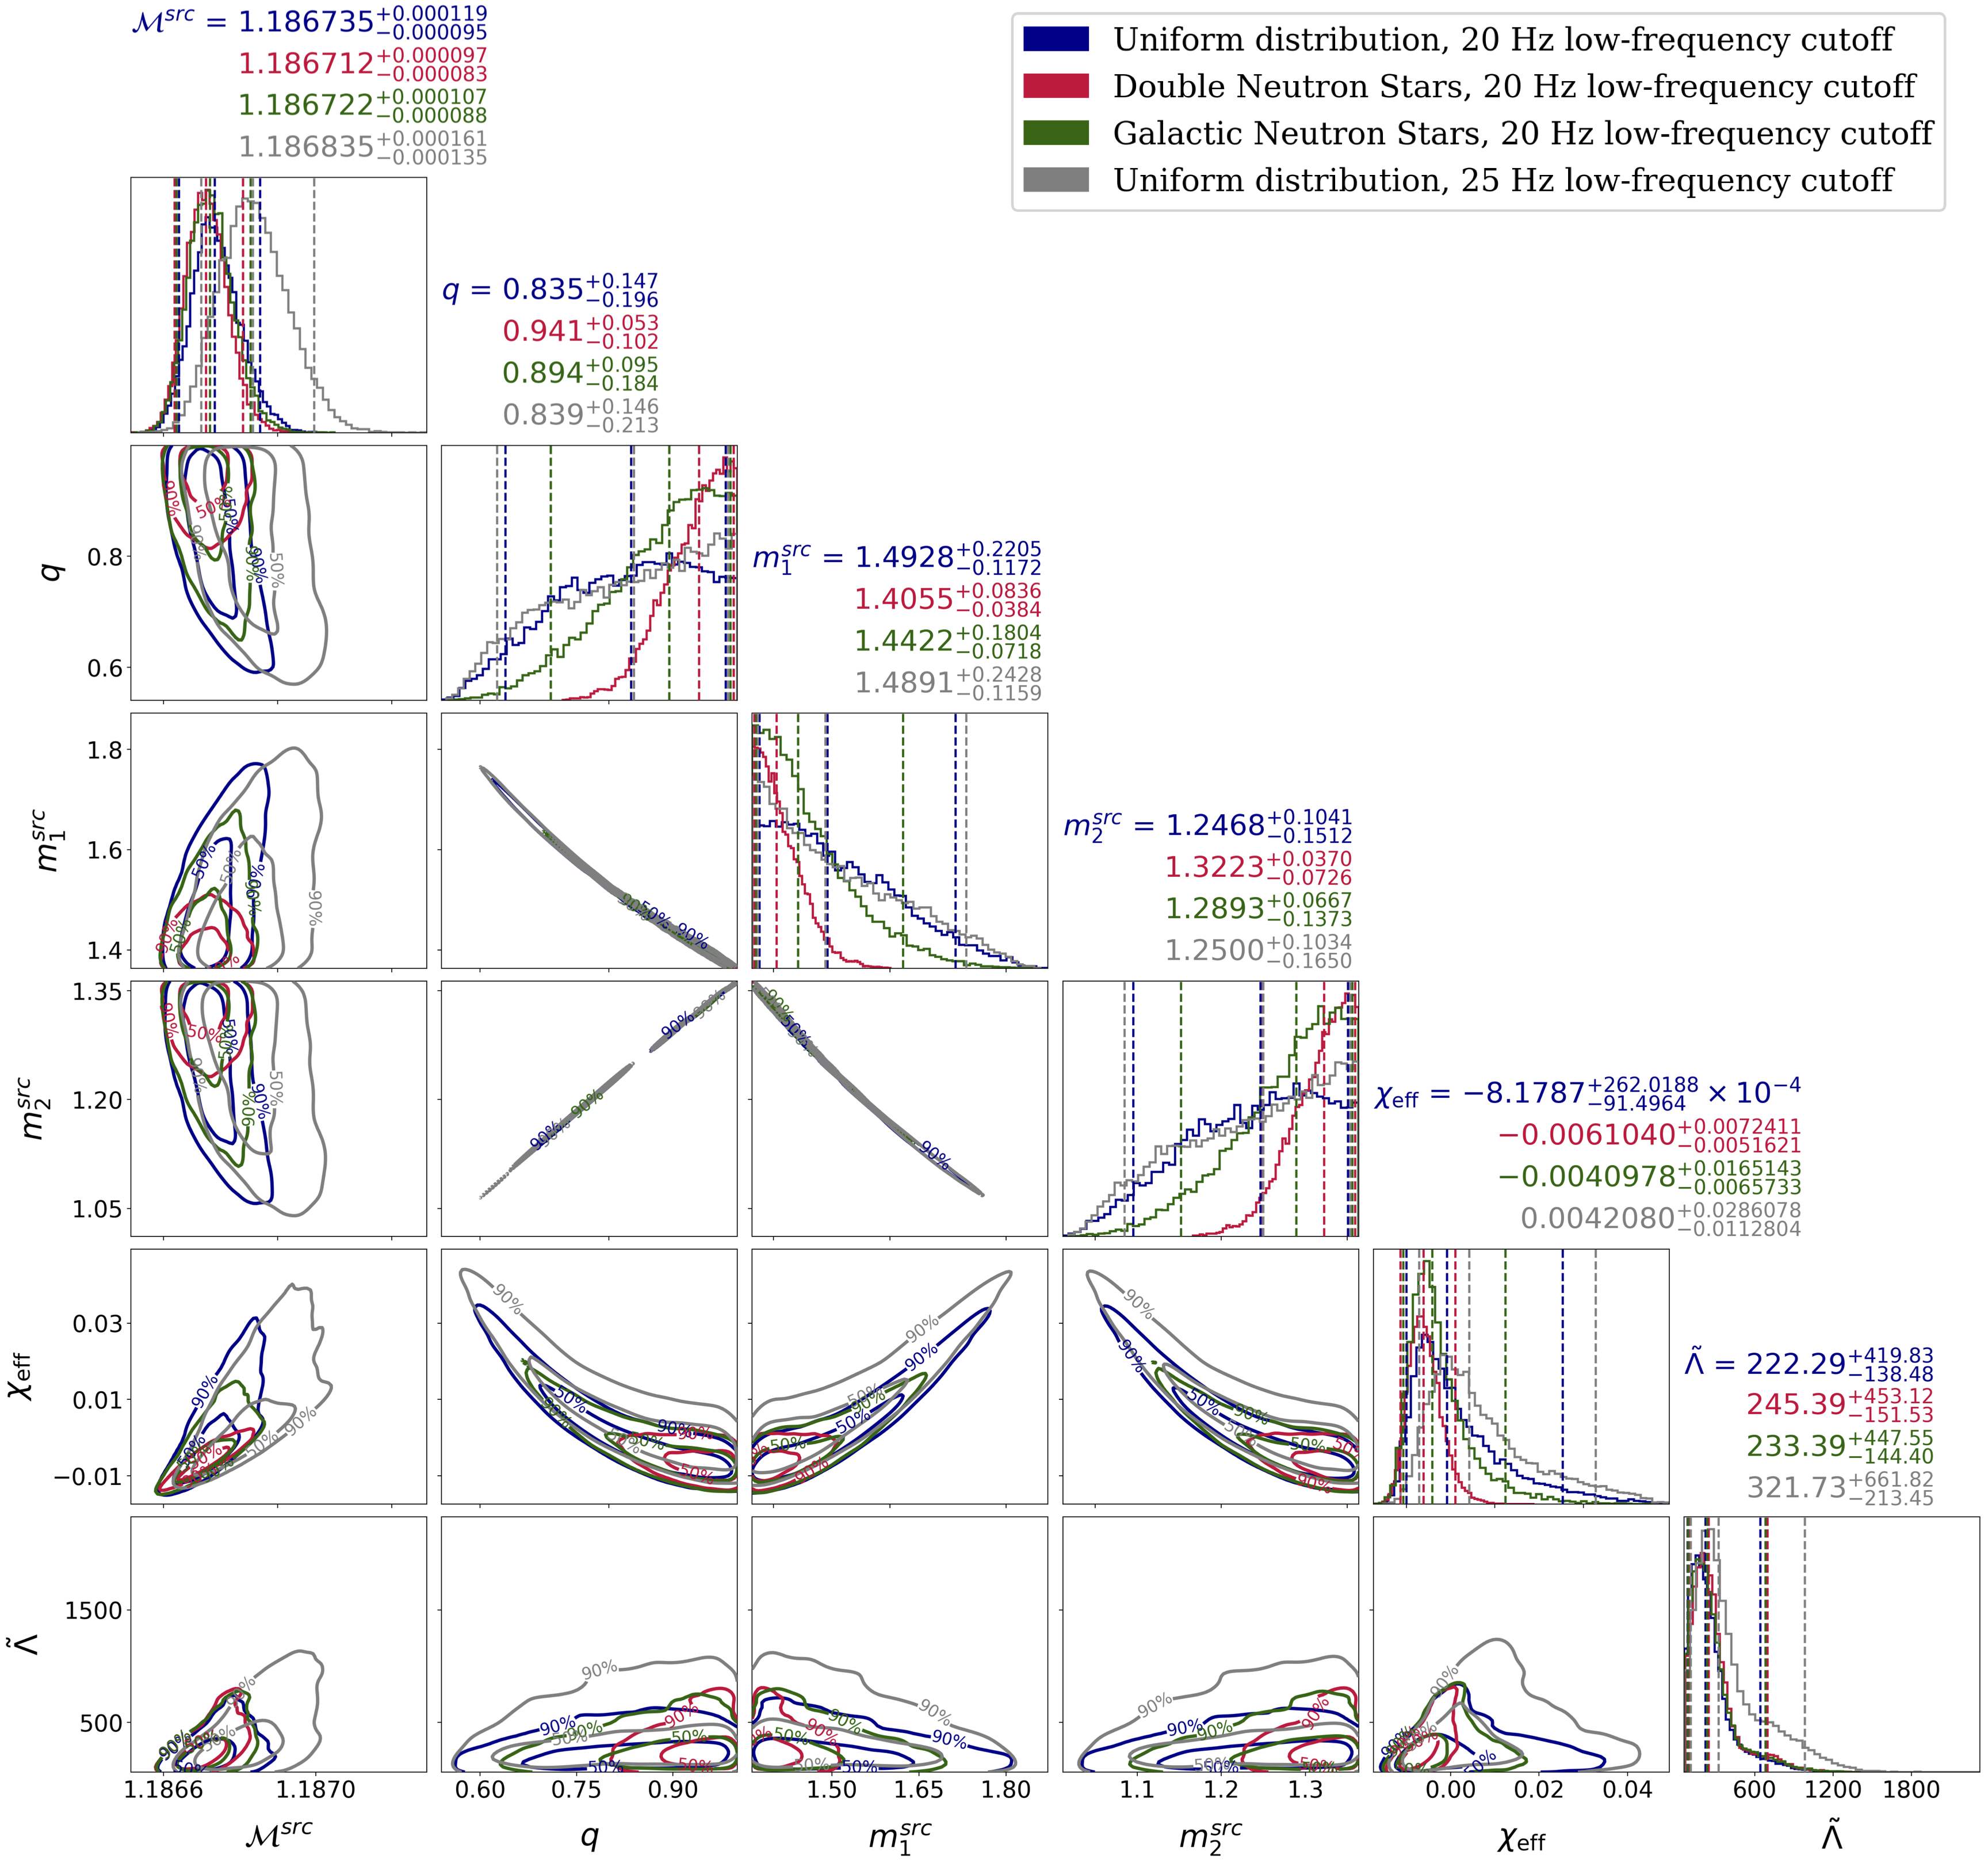
\includegraphics[max size={14cm}{14cm}]{figures/common_eos/posteriors_main_bothspins.png}
  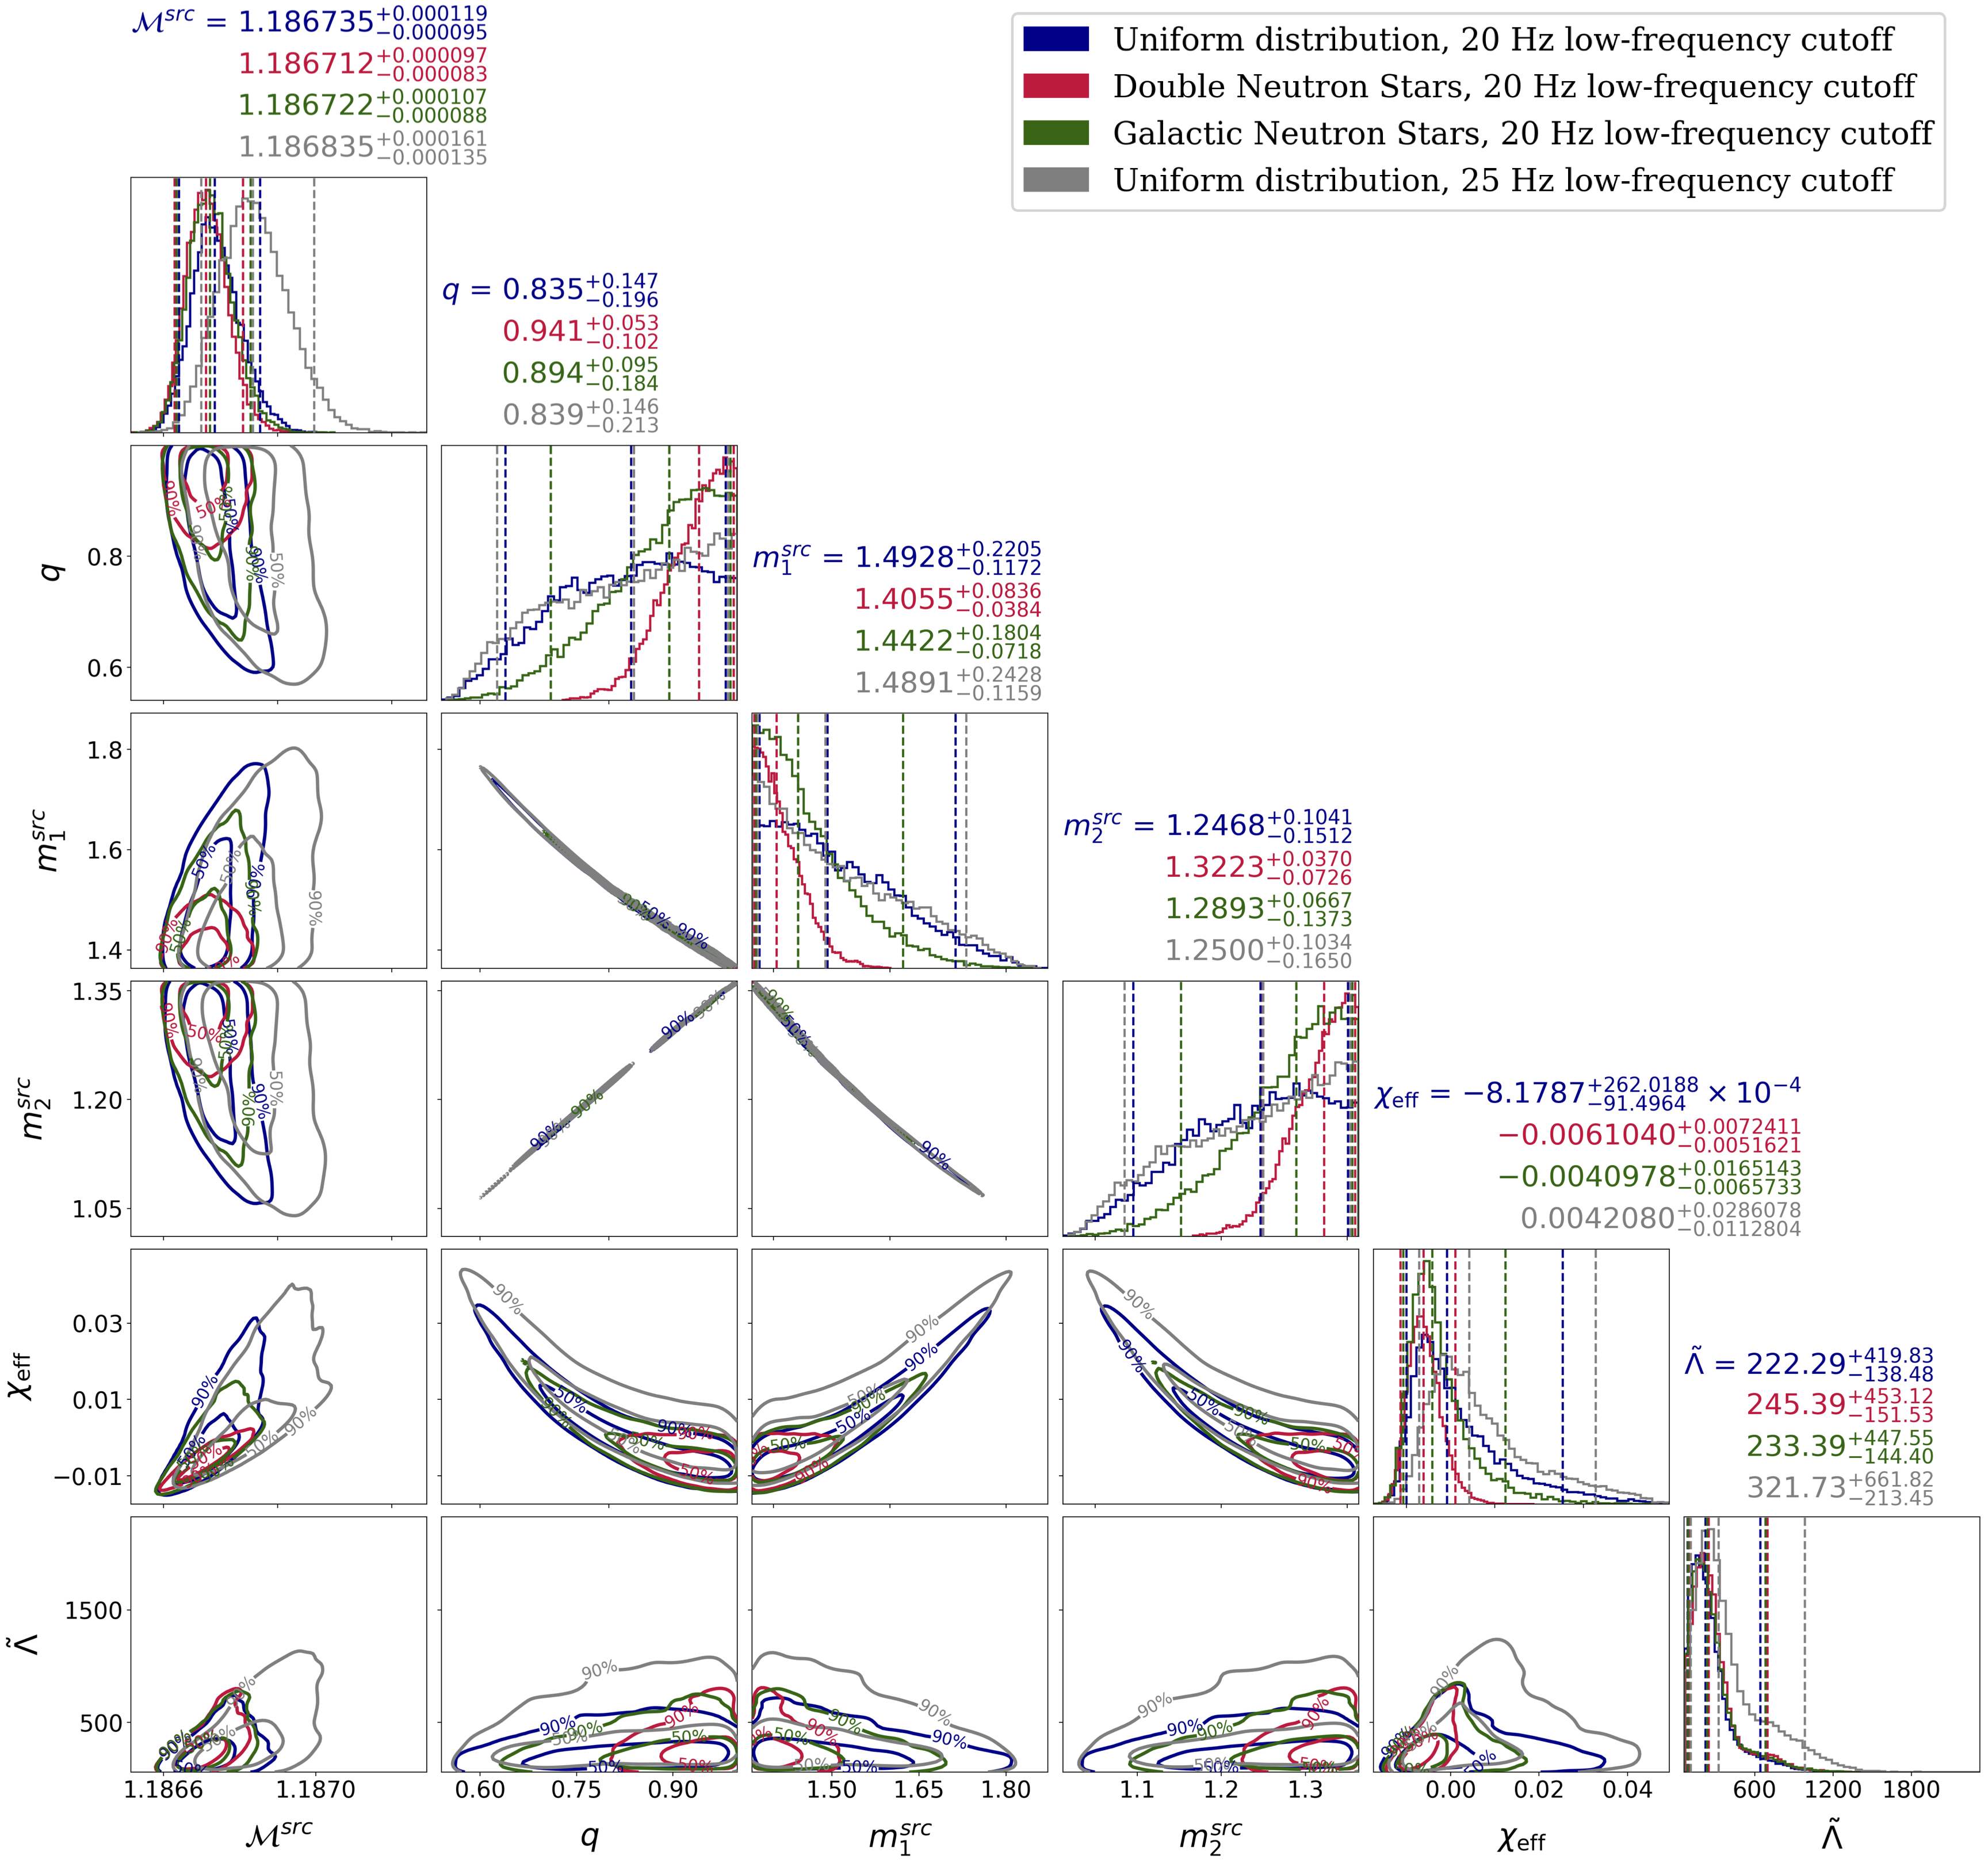
\includegraphics[width=\columnwidth]{figures/common_eos/posteriors_main_bothspins.png}
  \caption{\footnotesize Posterior distributions for the source frame chirp mass $\mathcal{M}^{\rm src}$, mass ratio $q$, source frame primary mass $m_1^{\rm src}$ and secondary mass $m_2^{\rm src}$, effective spin $\chi_{\rm eff}$, and binary deformability parameter $\tilde{\Lambda}$ from parameter estimation analyses with three different choices of mass priors. The posteriors represented in blue are from the analysis using a uniform prior on component masses, $m_{1,2} \sim U[1,2]\, M_\odot$, and 20~Hz low-frequency cutoff. The posteriors represented in red are from the analysis using a Gaussian mass prior for component masses $m_{1,2} \sim N(\mu = 1.33, \sigma = 0.09)\, M_\odot$ known from radio observations of neutron stars in double neutron star (DNS) systems, and 20~Hz low-frequency cutoff. The posteriors represented in green are from the analysis using the observed mass distributions of recycled and slow pulsars in the Galaxy with $m_1 \sim N(\mu = 1.54, \sigma = 0.23)\, M_\odot$ and $m_2 \sim N(\mu = 1.49, \sigma = 0.19)\, M_\odot$~\cite{Ozel:2016oaf}, and 20~Hz low-frequency cutoff. The posteriors represented in gray are from the analysis using a uniform prior on component masses, $m_{1,2} \sim U[1,2]\, M_\odot$, and 25~Hz low-frequency cutoff. All four analyses had the common EOS constraint and the causal $\Lambda(m)$ lower limit imposed. The one-dimensional plots show marginalized probability density functions for the parameters. The dashed lines on the one-dimensional histograms represent the 5$\%$, 50$\%$ and 95$\%$ percentiles for each analysis, the values of which are quoted in the titles of the histograms. The 2D plots show 50$\%$ and 90$\%$ credible regions for the different pairs of parameters. Comparison between the analyses with low-frequency cutoff 20~Hz (blue) and 25~Hz (gray) for the uniform mass prior case shows that extending from 25~Hz to 20~Hz better constrains $\mathcal{M}$, which improves the measurement of $\tilde\Lambda$ by eliminating a region of the posterior with higher values $\mathcal{M}$ and high $\tilde\Lambda$.
  \label{fig:posterior_overlap}}
%}}
\end{adjustwidth}
\end{figure}

Finally, we note the post-Newtonian waveform family used will result in systematic errors in our measurement of the tidal deformability \cite{Wade:2014vqa,Lackey:2014fwa}. However, this waveform family allows a direct comparison to the results of Ref.~\cite{TheLIGOScientific:2017qsa}. Accurate modeling of the waveform is challenging, as the errors in numerical simulations are comparable to the size of the matter effects that we are trying to measure~\cite{Barkett:2015wia}. Waveform systematics and comparison of other waveform models (e.g., \cite{Bernuzzi:2014owa}) will be investigated in a future work.

\begin{figure}[t]
  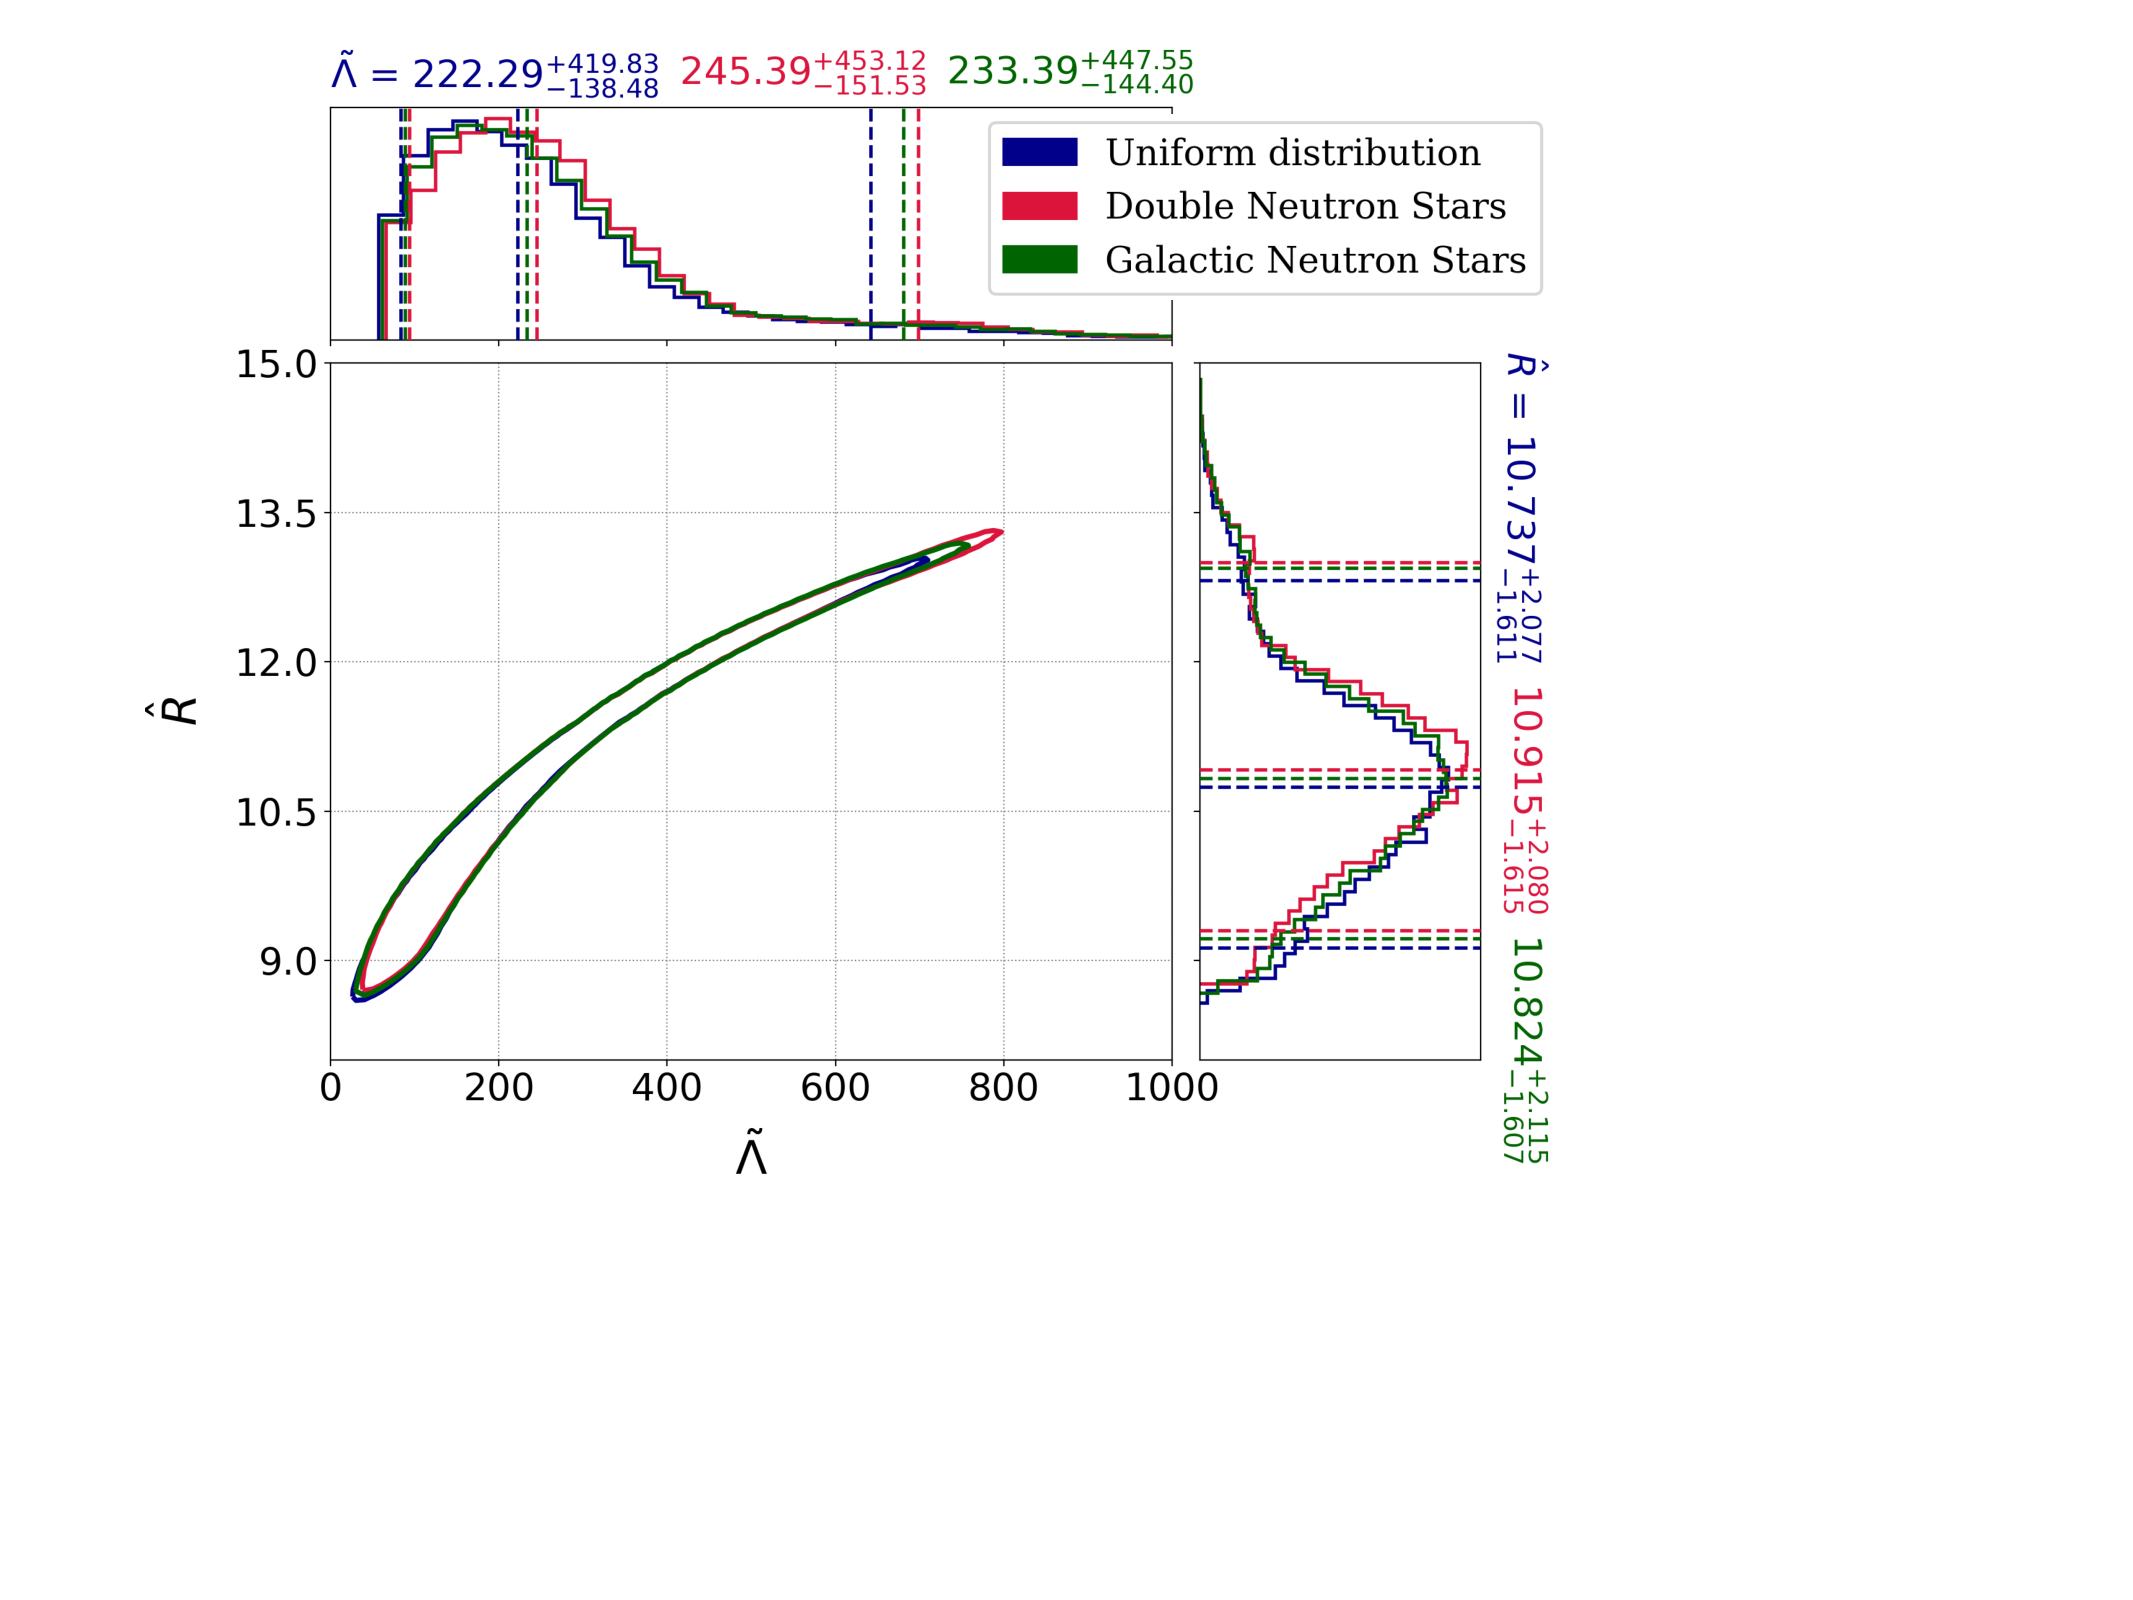
\includegraphics[width=\columnwidth]{figures/common_eos/Radius_lambda_bothspins.pdf}
  \caption{The 90\% credible region of the posterior probability for the common radius $\hat{R}$ and binary tidal deformability $\tilde\Lambda$ with the common EOS constraint for the three mass priors. The posteriors for the individual parameters are shown with dotted lines at  the 5$\%$, 50$\%$ and 95$\%$ percentiles. The values of $\tilde\Lambda$, and hence $\hat{R}$ forbidden by causality have been excluded from the posteriors. 
\label{fig:radius_lambda}%
%\vspace*{-0.5cm}%
}
\end{figure}

%\input{supp_common_eos.tex}

\section{Discussion}

Using Bayesian parameter estimation, we have measured the tidal deformability and common radius of the neutron stars in GW170817. Table~\ref{tab:summary_table} summarizes our findings.  To compare to Ref.~\cite{TheLIGOScientific:2017qsa}, which reports a 90\% upper limit on $\tilde\Lambda \le 800$ under the assumption of a uniform prior on $\tilde\Lambda$, we integrate the posterior for $\tilde{\Lambda}$ to obtain 90\% upper limits on $\tilde{\Lambda}$.   For the common EOS analyses, these are $485$, $521$, and $516$ for the uniform, double neutron star, and Galactic neutron star component mass priors, respectively. We find that, in comparison to the unconstrained analysis, the common EOS assumption significantly reduces the median value and 90\% confidence upper bound of $\tilde\Lambda$ by about 28\% and 19\%, respectively, for all three mass priors. The difference between our common EOS results for the three mass priors is consistent with the physics of the gravitational waveform. At constant $\mathcal{M}$, decreasing $q$ causes the binary to inspiral more quickly \cite{Hannam:2013uu}. At constant $\mathcal{M}$ and constant $q$, increasing $\tilde\Lambda$ also causes the binary to inspiral more quickly, so there is a mild degeneracy between $q$ and $\tilde\Lambda$. The uniform mass prior allows the largest range of mass ratios, so we can fit the data with a larger $q$ and smaller $\tilde\Lambda$. The double neutron star mass prior allows the smallest range of mass ratios, and so, a larger $\tilde\Lambda$ is required to fit the data, with the Galactic neutron star mass prior lying between these two cases. 

\begin{table}[t]\label{tab:parameters}
\setlength{\tabcolsep}{3.8pt}
\centering\begin{tabular}{lccc} 
\hline
\rule{0pt}{3ex}%
Mass prior \quad & \quad $\tilde{\Lambda}$ \quad & \quad $\hat{R}$ (km) \quad & \quad $\tilde{\Lambda}_{90\%}$\quad \\\hline
\rule{0pt}{3ex}%
Uniform & 222$^{+420}_{-138}$ & 10.7$^{+2.1}_{-1.6}\pm 0.2$ & $< 485$\\
Double neutron star & 245$^{+453}_{-151}$ & 10.9$^{+2.1}_{-1.6}\pm 0.2$ & $< 521$ \\
Galactic neutron star & 
233$^{+448}_{-144}$ & 10.8$^{+2.1}_{-1.6}\pm 0.2$ & $< 516$ \\
\hline
\end{tabular}
\caption{Results from parameter estimation analyses using three different mass prior choices with the common EOS constraint, and applying the causal minimum constraint to $\Lambda(m)$. We show 90$\%$ credible intervals for $\tilde{\Lambda}$, 90$\%$ credible intervals and systematic errors for $\hat{R}$, %Bayes factors $\mathcal{B}$ comparing our common EOS to the unconstrained results, 
and the 90\% upper limits on $\tilde\Lambda$.%
%\vspace*{-0.5cm}%
}
\label{tab:summary_table}
\end{table}
Nevertheless, considering all analyses we performed with different mass prior choices, we find a relatively robust measurement of the common neutron star radius with a mean value $\langle \large \hat R \rangle$ = 10.8 km bounded above by $\hat R < 13.2$~km and below by $\hat R > 8.9$~km. Nuclear theory and experiment currently predict a somewhat smaller range by 2 km but with approximately the same centroid as our results~\cite{Lattimer:2012nd,Lattimer:2012xj}. A minimum radius 10.5--11 km is strongly supported by neutron matter theory~\cite{Gandolfi:2011xu,Lynn:2015jua,Drischler:2015eba}, the unitary gas~\cite{Kolomeitsev:2016sjl}, and most nuclear experiments~\cite{Lattimer:2012nd,Lattimer:2012xj,Tews:2012fj}. The only major nuclear experiment that could indicate radii much larger than 13 km is the PREX neutron skin measurement, but this has published error bars much larger than previous analyses based on antiproton data, charge radii of mirror nuclei, and dipole resonances. 
Our results are consistent with photospheric radius expansion measurements of x-ray binaries which obtain $R \approx 10$--$12$~km~\cite{Ozel:2016oaf,Steiner:2010fz,Degenaar:2018lle}. Reference~\cite{Guillot:2014lla} found from an analysis of five neutron stars in quiescent low-mass x-ray binaries a common neutron star radius $9.4\pm1.2$ km, but systematic effects including uncertainties in interstellar absorption and the neutron stars' atmospheric compositions are large. Other analyses have inferred $12\pm0.7$~\cite{Lattimer:2013hma} and $12.3\pm1.8$ km~\cite{Shaw:2018wxh} for the radii of $1.4M_\odot$ quiescent sources. 

We have found that the relation $q^{7.48} < \Lambda_1/\Lambda_2 < q^{5.76}$, in fact, completely bounds the uncertainty for the range of $\mathcal{M}$ relevant to GW170817, assuming $m_2 > 1M_\odot$ \cite{Zhao:2018nyf} and that no strong first-order phase transitions occur near the nuclear saturation density (i.e., the case in which $m_1$ is a hybrid star and $m_2$ is not). Analyses using this prescription instead of the $q^6$ correlation produce insignificant differences in our results. Since models with the common EOS assumption are highly favored over those without this assumption, our results support the absence of a strong first-order phase transition in this mass range.

In this Letter, we have shown that, for binary neutron star mergers consistent with observed double neutron star systems~\cite{Tauris:2017omb}, assuming a common EOS implies that $\Lambda_1 / \Lambda_2 \simeq q^6$. We find evidence from GW170817 that favors the common EOS interpretation compared to uncorrelated deformabilities. Although previous studies have suggested that measurement of the tidal deformability is sensitive to the choice of mass prior \cite{Agathos:2015uaa}, we find that varying the mass priors does not significantly influence our conclusions suggesting that our results are robust to the choice of mass prior. Our results support the conclusion that we find the first evidence for finite size effects using gravitational-wave observations. 

Recently, the LIGO/Virgo collaborations have placed new constraints on the radii of the neutron stars using GW170817~\cite{Abbott:2018exr}. The most direct comparison is between our uniform mass prior result ($\hat R = 10.7^{+2.1}_{-1.6} \pm 0.2$) and the LIGO/Virgo method that uses equation-of-state-insensitive relations~\cite{Yagi:2016qmr,Chatziioannou:2018vzf} ($R_1 = 10.8^{+2.0}_{-1.7}$ and $R_2 = 10.7^{+2.1}_{-1.5}$~km). This result validates our approximation $R_1=R_2$ used to motivate the prescription $\Lambda_1=q^6\Lambda_2$, and Eqs.~(\ref{eq:lambda_t1}, \ref{eq:lambda_t2}). Our statistical errors are comparable to the error reported by LIGO/Virgo. Systematic errors from EOS physics of $\pm 0.2$~km are added as conservative bounds to our statistical errors, broadening our measurement error, whereas Ref.~\cite{Abbott:2018exr} marginalized over these errors in the analysis. Reference~\cite{Abbott:2018exr} also investigates a method of directly measuring the parameters of the EOS which results in smaller measurement errors. Investigation of these differences between our analysis and the latter approach will be pursued in a future paper. 

Observations of future binary neutron star mergers will allow further constraints to be placed on the deformability and radius, especially if these binaries have chirp masses similar to GW170817 as radio observations suggest. As more observations improve our knowledge of the neutron star mass distribution, more precise mass-deformability correlations can be used to further constrain the star's radius.

%\clearpage
%\newpage

%\onecolumngrid
%\begin{center}
%{\large \bf Supplemental Material}
%\vspace*{1cm}
%\twocolumngrid
%\end{center}

%\clearpage
%\newpage

%\onecolumngrid
%\begin{center}
%{\large \bf Erratum}
%\vspace*{1cm}
%\twocolumngrid
%\end{center}

%\input{erratum_common_eos.tex}
\Chapter{Common Envelope Wind Tunnel: The effects of binary mass ratio and implications for the accretion-driven growth of LIGO binary black holes}
\label{ch:common_envelope}
We present three-dimensional local hydrodynamic simulations of flows around objects embedded within stellar envelopes using a ``wind tunnel'' formalism. Our simulations model the common envelope dynamical inspiral phase in binary star systems in terms of dimensionless flow characteristics. We present suites of simulations that study the effects of varying the binary mass ratio, stellar structure, equation of state, relative Mach number of the object's motion through the gas, and density gradients across the gravitational focusing scale. For each model, we measure coefficients of accretion and drag experienced by the embedded object. These coefficients regulate the coupled evolution of the object's masses and orbital tightening during the dynamical inspiral phase of the common envelope. We extrapolate our simulation results to accreting black holes with masses comparable to that of the population of LIGO black holes. We demonstrate that the mass and spin accrued by these black holes per unit orbital tightening are directly related to the ratio of accretion to drag coefficients. We thus infer that the mass and dimensionless spin of initially non-rotating black holes change by of order 1\% and 0.05, respectively, in a typical example scenario. Our prediction that the masses and spins of black holes remain largely unmodified by a common envelope phase aids in the interpretation of the properties of the growing observed population of merging binary black holes. Even if these black holes passed through a common envelope phase during their assembly, features of mass and spin imparted by previous evolutionary epochs should be preserved.

\section{Introduction} \label{sec:intro}
A common envelope phase is a short episode in the life of a binary star system in which the two components of the binary evolve inside a shared envelope. Common envelope phases typically occur when one of the stars in the binary expands, engulfing its companion object \cite{Paczynski:1976,1978ApJ...222..269T,1993PASP..105.1373I,2010NewAR..54...65T,2013A&ARv..21...59I,2017PASA...34....1D}. Inside the common envelope, the embedded companion object interacts with the material flowing past it, giving rise to dynamical friction drag forces \cite{1943ApJ....97..255C,1999ApJ...513..252O}. These drag forces lead to an orbital tightening as the two objects spiral in. 
Common envelope phases are thought to be critical to the formation of compact-object binaries that subsequently merge through the emission of gravitational radiation~\cite{Heuvel:1976,Smarr:1976} (see, e.g., \cite{Mandel:2018hfr}, for a review). Thus, understanding the common envelope phase is important for understanding the formation channel and evolutionary history of merging compact-object binaries, such as those observed by the LIGO and Virgo gravitational-wave detectors \cite{TheLIGOScientific:2014jea, TheVirgo:2014hva}.

Significant theoretical effort has gone into modeling the physical processes of common envelope phases. This work has been challenging because of the range of physically-significant spatial and temporal scales, as well as the range of potentially important physical processes \cite{1993PASP..105.1373I,2013A&ARv..21...59I}. One crucial example is the energy release from the recombination of ionized hydrogen and helium \cite{Nandez:2015,Ivanova:2016,Lucy:1967,Roxburgh:1967,Han:1994,Han:2002}.  Efforts have often either focused on global hydrodynamic modeling of the overall encounter (for example, the recent work of \cite{Ricker_2007,Passy_2011,Ricker_2012,Ohlmann:2016a,Ohlmann:2016b,Iaconi:2017,Iaconi:2018,Chamandy:2018,Chamandy:2018a,Reichardt:2019,Chamandy:2019psk,Fragos:2019box}), 
or local hydrodynamic simulations that simplify and zoom in on one aspect of the larger encounter (e.g., \cite{Fryxell:1987,Fryxell:1988,Taam:1989,Sandquist_1998,MacLeod_2015,MacLeod:2014yda,MacLeod:2017}). 

Global simulations attempt to model the full spatial extent of binary systems for many orbital timescales. This approach captures the full extent of the envelope structure and the physical complexities involved. However, this also leads to the simulations being highly computationally expensive, limiting the choice to exploring a small parameter space with high resolution, or exploring a large parameter space with low resolution. Local simulations, on the other hand, attempt to isolate and study flow morphologies around the embedded object with a broad parameter space and high resolution. This approach does not capture the full geometry in a single simulation. However, the goal is to model flow conditions representative of different regions or times within the overall event. Adding together results from multiple such simulations can help to interpret the outcomes of global models and physics of the full common envelope interaction.
A synthesis of the global and local simulations offers a pathway toward understanding the complex gas dynamics of common envelope phases.

This paper extends previous work on local simulations of gas flow past an object inspiraling through the gaseous surroundings of a common envelope. We use the ``wind tunnel'' formalism, first presented in Ref. \cite{MacLeod:2014yda}, and expanded in Ref. \cite{MacLeod:2017} to study the flow past a compact object embedded in the stellar envelope of a red giant or asymptotic giant branch star. The stellar profile of the donor at the onset of the dynamically unstable mass transfer depends on the mass ratio and initial separation between the centers of the two stars in the binary. 
We focus in particular on the variation in the properties as the binary mass ratio changes, and we present two suites of simulations with ideal gas equations of state characterized by adiabatic exponents $\gamma = 4/3$ and $\gamma = 5/3$, which bracket the range of typical values in stellar envelopes (e.g., \cite{MacLeod:2017,Murguia-Berthier:2017}).

This paper is organized as follows. In Sec.~\ref{sec:CE_params} we describe the common envelope flow parameters and conditions. We describe gravitational focusing in common envelope flows and illustrate the parameter space that controls the properties of the local flow past an object embedded in a common envelope. In Sec.~\ref{sec:hydro_sims} we describe the wind tunnel setup for hydrodynamic simulations, describe the model parameters, illustrate how the flow evolves through the simulations, and the quantities that we compute as a product of the simulations. We present hydrodynamic simulations using the wind tunnel setup for common envelope flows with a $\gamma = 4/3$ and $\gamma = 5/3$ equation of state, describe the flow characteristics, and the results obtained from the simulations. In Sec.~\ref{sec:implications}, we extrapolate our simulation results for the scenario of a black hole inspiraling through the envelope of its companion. We estimate the mass and spin accrued by black holes during the common envelope phase and derive implications for the effect of this phase on the properties of black holes in merging binaries that constitute LIGO-Virgo sources.
We conclude in Sec.~\ref{sec:conclusions}. A companion paper, Ref. \cite{Rosa:2020}, explores the validity of the expression of realistic stellar models in the dimensionless terms adopted here.

\vspace{5mm}
\section{Common envelope flow parameters and conditions}\label{sec:CE_params} 

\subsection{Characteristic Scales}
%The Hoyle-Lyttleton (HL) theory of accretion ~\cite{1939PCPS...35..405H,1944MNRAS.104..273B,Edgar:2004}, is used extensively to describe accretion onto a compact object having a velocity relative to the ambient medium. We use that as a starting point to consider an embedded, accreting object of mass $M_2$ moving with velocity $v_{\infty}$ relative to a surrounding gas of unperturbed density $\rho_\infty$ that follows a stellar profile typical of a common envelope. The characteristic impact parameter inside which gas is gravitationally focused toward the embedded object and can potentially accrete is 
%\begin{equation}
%R_{\mathrm a} = \frac{2GM_2}{v_{\infty}^{2}},
%\end{equation}
%which implies a characteristic interaction cross section of $\pi R_{\mathrm{a}}^2$ \cite{1939PCPS...35..405H}. 
The Hoyle-Lyttleton (HL) theory of accretion ~\cite{1939PCPS...35..405H,1944MNRAS.104..273B,Edgar:2004}, is used extensively to describe accretion onto a compact object having a velocity relative to the ambient medium. We use that as a starting point to consider an embedded, accreting object of mass $M_2$ moving with velocity $v_{\infty}$ relative to a surrounding gas of unperturbed density $\rho_\infty$ that follows a stellar profile typical of a common envelope. The characteristic impact parameter inside which gas is gravitationally focused toward the embedded object and can potentially accrete is set by the Bondi-Hoyle accretion radius, written as
\begin{equation}
R_{\rm{a, BH}} = \frac{2GM_2}{v_{\infty}^{2} + c_{s, \infty}^{2}}.
\end{equation}
For an object in significantly supersonic motion $v_{\infty} >$ $c_{s, \infty}$, where $c_{s, \infty}$ is the sound speed of the gas, the Bondi-Hoyle accretion radius can be replaced by the Hoyle-Lyttleton accretion radius, written as
\begin{equation}
R_{\rm{a, HL}} = \frac{2GM_2}{v_{\infty}^{2}}.
\end{equation}

During the dynamical inspiral phase of common envelope evolution for a system consisting of a black hole in a red supergiant, the embedded object moves supersonically through the host envelope (e.g. \cite{MacLeod_2015}). This scenario can be appropriately described by Hoyle-Lyttleton scales (with accretion radius $R_{\rm a, HL}$), and this is the regime that we model in this work. We refer to $R_{\rm a, HL}$ as $R_{\rm a}$, henceforth.

Hoyle-Lyttleton accretion implies a characteristic interaction cross section of $\pi R_{\mathrm{a}}^2$ \cite{1939PCPS...35..405H}.
The corresponding mass flux through this cross section, and potential mass accretion rate in HL flows can be written as~\cite{Edgar:2004},
\begin{equation}\label{eq:mdotHL}
\dot M_{\rm HL} = \pi R_{\mathrm{a}}^2 \rho_\infty v_\infty. 
\end{equation}
The characteristic scales for momentum and energy dissipation due to gravitational interaction \cite{1999ApJ...513..252O} can be derived from this cross section as well. The characteristic scale for the momentum dissipation rate, or force, is
\begin{equation}\label{eq:fHL}
    F_{\rm HL} = \pi R_{\mathrm{a}}^2 \rho_\infty v_\infty^2 = \dot M_{\rm HL} v_\infty, 
\end{equation}
and the characteristic energy dissipation rate is
\begin{equation}
    \dot E_{\rm HL} = \pi R_{\mathrm{a}}^2 \rho_\infty v_\infty^3 = \dot M_{\rm HL} v_\infty^2, 
\end{equation}
if we assume that all momentum and energy passing through the interaction cross section $\pi R_{\mathrm{a}}^2$ are dissipated. 

\subsection{Common Envelope Parameters}

We imagine that the embedded object $M_2$ is spiralling in to tighter orbital separations within the envelope of a giant-star primary.  The core of the primary is fixed at $r = 0$ and the orbital radius of $M_2$ within  the primary's envelope is $r = a$. Thus, the stellar cores are separated by a distance $a$, smaller than the original radius of the primary.  We use $M_1(r)$ to denote the mass of the primary that is enclosed by the orbit of $M_2$. Therefore, the Keplerian orbital velocity is $v_{\rm k} = \sqrt{GM/a}$,
where $M = M_{1}(a) + M_{2}$ is the total enclosed mass of the binary (mass outside of the orbital separation $a$ does not contribute to the orbital velocity). The relative velocity of the secondary to the envelope gas, $v_{\infty}$, is related to the Keplerian velocity of the secondary as $v_{\infty} = f_{\rm k}v_{k}$. Thus, $f_{\rm k}$ is the fraction of the Keplerian velocity that contributes to the relative velocity. In our simulations, we adopt the simplification $f_{\rm k} = 1$. However, $f_{\rm k} < 1.0$ is possible if the orbital motion of the embedded object is partially synchronized to the donor's envelope.

Given a relative velocity set by the orbital motion, the ratio of the gravitational focusing scale, $R_{\rm a}$, to the orbital separation, $a$, is \cite{MacLeod:2017}
\begin{equation}
\frac{R_{\mathrm a}}{a} = \frac{2}{f_{\rm k}^{2}}\frac{M_{2}}{M} = \frac{2}{f_{\rm k}^{2}}\frac{1}{1 + q_{\rm r}^{-1}},\label{eq:Ra_asfunc_a}
\end{equation}
where $q_{\rm r}=M_{2}/M_{1}(r)$ is the mass ratio between the embedded object and the mass enclosed by its orbit. Therefore, for a given value of $q_{\rm r}$, one can calculate $R_{\mathrm a}$ in terms of $a$. The variation of $R_{\mathrm a}$ in terms of $a$ with $q_{\rm r}$ is shown in Figure~\ref{fig:ra-q} for $f_{\rm k}=1, 0.9, 0.8$. As $q_{\rm r}$ increases, $R_{\mathrm a}/a$ also increases, and gives an approximate scale for the fraction of the envelope affected by the embedded object.

The HL formalism assumes a homogeneous background for the embedded object. In practice, such a situation does not arise in common envelope encounters. As demonstrated in Figure \ref{fig:ra-q},  $R_{\mathrm{a}}/a$ can be a large fraction of unity for typical mass ratios. Therefore, the gaseous medium with which the embedded object interacts spans a range of densities and temperatures \cite{MacLeod_2015}. 

\begin{figure}[t]
  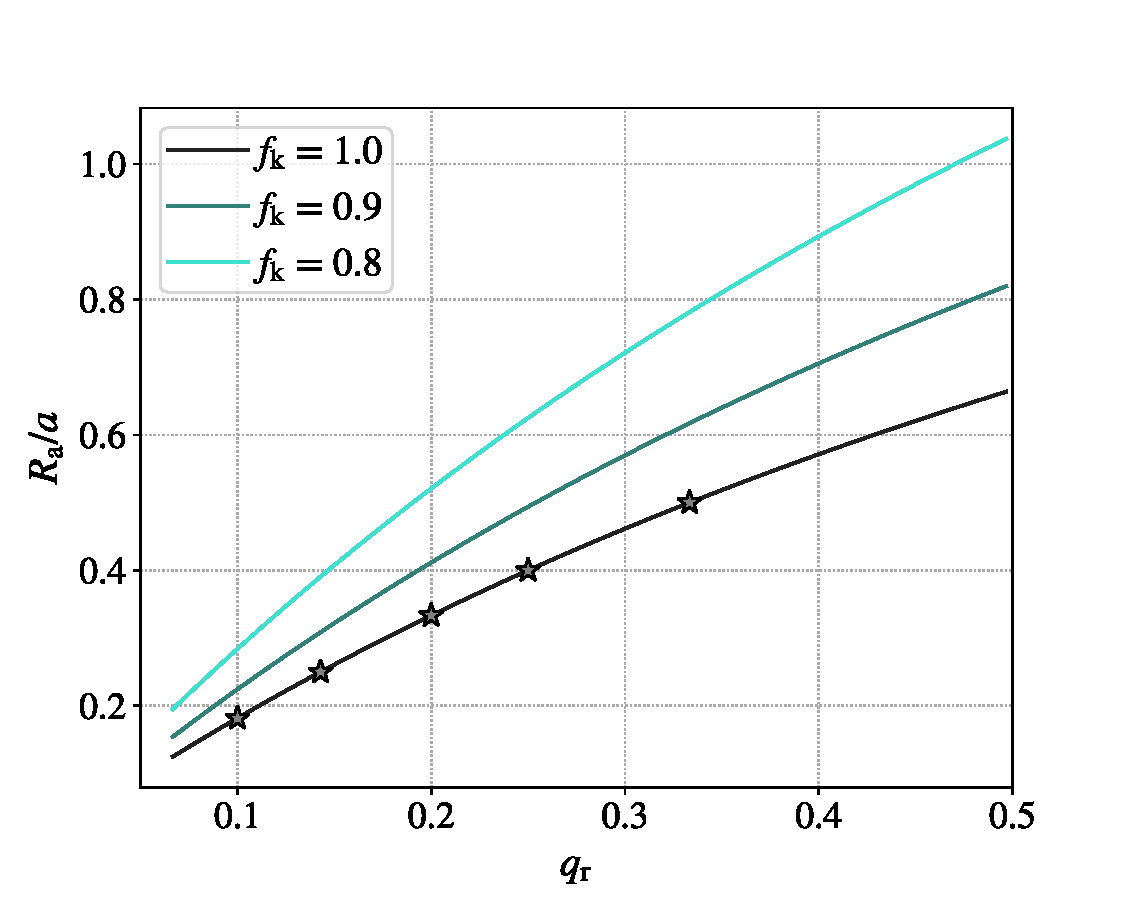
\includegraphics[width=\columnwidth]{figures/common_envelope/ra-q_3fks.pdf}
 \caption{Fraction of the orbital separation falling within the gravitational focusing radius of the embedded object, $R_{\rm a}/a$, as a function of the binary mass ratio $q_{\rm r}$. The plot shows the relation for $f_{\rm k} = 1.0, 0.9, 0.8$, where $f_{\rm k}$ is the fraction of the Keplerian velocity contributing to the relative velocity. Markers show the points for which hydrodynamical simulations have been performed in this paper. For small mass ratios, the accretion radius of $M_2$ is small relative to the orbital separation.  When $q_{\rm r}$ is large, $R_a$ sweeps out a significant fraction of the orbital separation.  For fixed $M_2$, $q_{\rm r}$  increases as the  embedded object spirals further into the envelope of the primary.
 \label{fig:ra-q}}
\vspace{5mm}
\end{figure}

The flow upstream Mach number is the ratio of orbital velocity to sound speed, 
\begin{equation}
\mathcal{M}_\infty = \frac{v_\infty}{c_{s, \infty}},
\end{equation}
where we specify $c_{s, \infty}$ to be the sound speed measured at radius $r=a$ within the common envelope gas. 
Furthermore, the density gradient in stellar profiles can be expressed in terms of a local density scale height at the location of the embedded object as
\begin{equation}
H_\rho = -\rho \frac{dr}{d\rho} . 
\end{equation}
The number of scale heights encompassed by the accretion radius is then quantified by the ratio
\begin{equation}
\epsilon_\rho = \frac{R_{\mathrm{a}} }{ H_\rho} ,    
\end{equation}
which is, like other quantities, evaluated at the location of the embedded object. This density gradient breaks the symmetry of the flow envisioned in the HL scenario and gives the flow a net angular momentum relative to the accreting object \cite{MacLeod_2015,MacLeod:2014yda,MacLeod:2017,Murguia-Berthier:2017}.

Ref. \cite{MacLeod:2017} showed that there is a clear relation between Mach number and density gradient for typical common envelope flows when the (local) envelope structure is approximated as a polytrope with index 
\begin{equation}
\Gamma_{\rm s} = \bigg(\frac{d\ln{P}}{d\ln{\rho}}\bigg)_{\rm envelope}.
\end{equation}
Under the simplification of an ideal gas equation of state with adiabatic index $\gamma$, we can rewrite the hydrostatic equilibrium condition of the envelope as a relationship between $\mathcal{M}_\infty$ and $\epsilon_\rho$ (Equation 18 of \cite{MacLeod:2017}, 
\begin{equation}\label{eq:mach-erho}
\mathcal{M}^2_\infty = \epsilon_\rho \frac{(1 + q_{\rm r})^2}{2q_{\rm r}}f_{\rm k}^4 \bigg(\frac{\Gamma_s}{\gamma}\bigg).
\end{equation}
This relation reduces the parameter space to a set of specific combinations of $\epsilon_\rho$, $\mathcal{M}_\infty$, $q_{\rm r}$ values, that are realized in common envelope phases.
%Thus, not all parameter combinations of $\mathcal{M}_\infty$ and $\epsilon_\rho$ are realized in common envelope phases. %\textcolor{red}{\textit{Soumi: Should we remove this line?} Instead, typical parameter combinations are $f_{\rm k}$ and $q_{\rm r}$}.
The validity of this approximation in the context of detailed stellar evolution models  is  discussed  in Ref. \cite{Rosa:2020}, who argue that the simulations presented in this paper are still applicable to a wide range of detailed stellar models described by a realistic equation of state.

\vspace{0.5cm}
\section{Hydrodynamic Simulations\label{sec:hydro_sims}}
In this section we describe hydrodynamic simulations in the Common Envelope Wind Tunnel formalism \cite{MacLeod:2017} that explore the effects of varying the binary mass ratio on coefficients of drag and accretion realized during the dynamical inspiral of an object through the envelope of its companion.  

\subsection{Numerical Method}\label{sec:method}
The Common Envelope Wind Tunnel model used in this work is a hydrodynamic setup using the FLASH Adaptive Mesh Refinement hydrodynamics code \cite{Fryxell2000}. A full description of the model is given in Section 3 of Ref. \cite{MacLeod:2017}. The basic premise is that the complex geometry of a full common envelope scenario is replaced with a 3D Cartesian wind tunnel surrounding a hypothetical embedded object. Flow moves past the embedded object and we are able to measure rates of mass accretion and drag forces. 

In the Common Envelope Wind Tunnel, flows are injected from the $-x$ boundary of the computational domain past a gravitating point mass, located at the coordinate origin of the three-dimensional domain.  To simulate accretion, the point mass is surrounded by a low pressure ``sink" of radius $R_{\rm s}$. The gas obeys an ideal gas equation of state $P=(\gamma-1)\rho e$, where $e$ is the specific internal energy. The profile of inflowing material is defined by its upstream Mach number, $\mathcal M_\infty$, and the ratio of the accretion radius to the density scale height, $\epsilon_\rho$.  Calculations are performed in code units $R_{\mathrm{a}} = v_\infty = \rho_\infty = 1$. Here $\rho_\infty$ is the density of the unperturbed profile at the location of the embedded object. This gives a time unit of $R_{\mathrm{a}}/v_\infty = 1$, which is the time taken by the flow to cross the accretion radius. The binary separation $a$ in code units is
\begin{equation}\label{eq:sepcode}
\frac{a}{R_{\rm a}} = \frac{1}{2}f_{\rm k}^2 (1 + q_{\rm r}^{-1}) .
\end{equation}
The density profile of the gas in the $\hat y$-direction is that of a polytrope with index $\Gamma_s$ in hydrostatic equilibrium with a gravitational force 
\begin{equation}
\vec{a}_{\rm grav, 1} = -\frac{GM_1(r)}{(y - y_1)^2}\hat{y},
\end{equation}
that represents the gravitational force from the primary star's enclosed mass, $M_1 (r)$. The density scale height, sound speed and upstream Mach number vary across this profile as they would in a polytropic star.  At the $+y$ and $\pm z$ boundaries, a ``diode'' boundary condition is applied, that allows material to leave but not enter into the domain. 


The size of the domain is set by the mass ratio of the binary system and the effective size of the binary orbit, as described by Equation \eqref{eq:sepcode}. Gravitationally focused gas flows are sensitive to the distance over which they converge, and the size of the wake that they leave (e.g. \cite{1999ApJ...513..252O}). In varying the binary mass ratio, it is important to capture this physical property of differing ratio of the gravitational focus radius to the physical size of the system, equation \eqref{eq:sepcode}. In order to capture the full flow, our domain has a diameter equal to the binary separation $a$, implying that it extends a distance $\pm a/2 =  (1 + q_{\rm r}^{-1}) R_{\mathrm{a}}/4$ about the origin in the $\pm x$, $\pm y$, and $\pm z$ directions. 
  
This domain is spatially resolved by  cubic blocks that have extent of $R_{\rm a}/2$ in each direction, and each block is made of $8^3$ zones. The largest zones have length $R_{\mathrm{a}}/16$. We allow for five levels of adaptive mesh refinement, giving the smallest zones length $R_{\mathrm{a}}/256$. We enforce maximum refinement around the embedded object at all times.  


\subsection{Model Parameters}

The simulations that we present later in this section assume $\Gamma_s = \gamma$ and $f_{\rm k} = 1$. We are therefore modeling constant entropy stellar envelope material (as in a convective envelope of a giant star) and relative velocities between the embedded object and the background gas equal to the Keplerian velocity. All models adopt a sink radius for measuring accretion of $R_{\rm s} = 0.05R_{\mathrm{a}}$ around the embedded object. In Section \ref{sec:sink}, we perform simulations with varying sink radius and we discuss the dependence of our results on this parameter. 

This leaves three flow parameters in equation~\eqref{eq:mach-erho}: $\mathcal{M}_\infty$, $\epsilon_\rho$, and $q_{\rm r}$, only two of which can be chosen independently. Figure \ref{fig:parameterspace} shows the simulation grid presented in this paper and those in Refs. \cite{MacLeod:2014yda,MacLeod:2017} in the $\mathcal{M}_\infty - \epsilon_\rho$ space. The simulations in this paper expand the parameter space covered in the previous papers with a broader range of $\mathcal{M}_\infty$ (therefore $\epsilon_\rho$) and, crucially, models of varying mass ratio, $q_{\rm r}$. We construct a grid of $q_{\rm r} - \mathcal{M}_\infty$ values, with $q_{\rm r}$ values $1/10$, $1/7$, $1/5$, $1/4$, $1/3$. For each value of $q_{\rm r}$ we perform simulations with $\mathcal{M}_\infty$ of $1.15$, $1.39$, $1.69$, $2.2$, $2.84$, $3.48$, and $5.0$. It was shown in Ref. \cite{MacLeod_2015} with the help of MESA simulations of 1-16$M_\odot$ stars evolved from the zero-age main sequence to the giant branch expansion, that typical upstream Mach number values range from $\mathcal{M}_\infty~\approx 2$ in the deep interior to $\mathcal{M}_\infty \gtrsim 5$ near the stellar limb. Extending these results in Ref. \cite{Rosa:2020}, MESA is used to evolve a broader range of stellar masses 3--90$M_\odot$ with binary mass ratios of 0.1--0.35, finding $1.5 \lesssim \mathcal{M}_\infty < 7$ in giant branch stellar envelopes. It should be noted that the Mach numbers values discussed here and used as model parameters are defined upstream of the flow. Mach number values would differ when measured in the vicinity of the object, as material might then have crossed a shock and been compressed or heated, such as those measured in Ref. \cite{Iaconi:2018}.

\begin{figure}[t]
  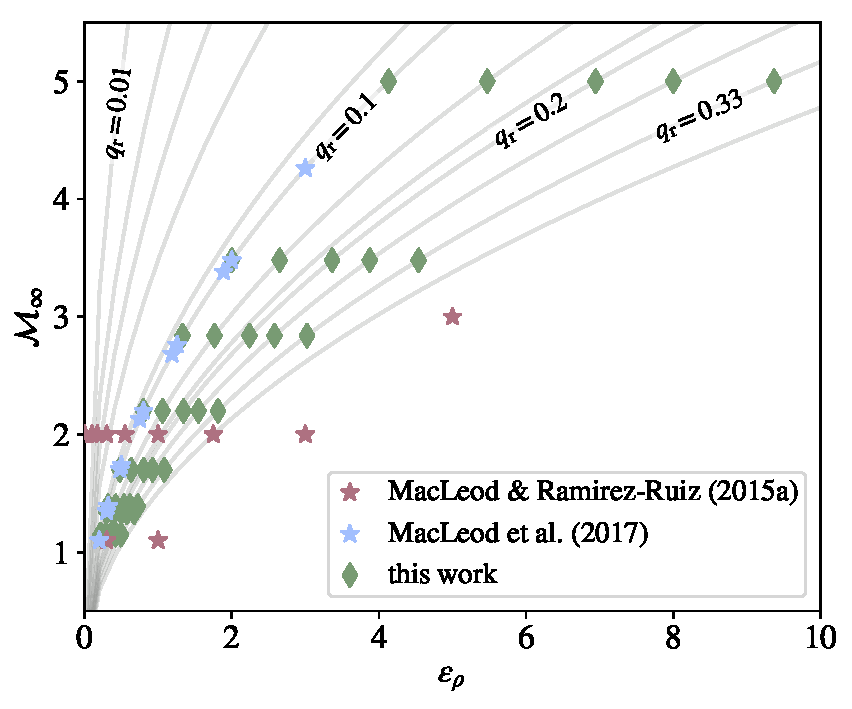
\includegraphics[width=\columnwidth]{figures/common_envelope/paramspace_v4.pdf}
 \caption{Points in the $\mathcal{M}_{\infty}$-$\epsilon_{\rho}$ space representing flow parameters for simulations performed with the ``wind tunnel'' setup. For polytropic envelopes, each combination of $\mathcal{M}_{\infty}$ and $\epsilon_{\rho}$ has a corresponding $q_{\rm r}$ value \cite{MacLeod:2017}. Simulations are shown on lines of constant $q_{\rm r}$, with the exception of three simulations from Ref. \cite{MacLeod_2015} that do not follow the polytropic relation. The simulations in this work expand upon the previous work as labeled, extending across both axes to higher Mach numbers and steeper density gradients, significantly extending coverage across the region of parameter space realized in realistic stellar profiles as detailed in Ref. \cite{Rosa:2020}.\label{fig:parameterspace}}
\vspace*{5mm}
\end{figure}

Tabulated model parameters are presented in Table~\ref{tab:sims_43_params} and Table~\ref{tab:sims_53_params}. We divide our discussion in the subsequent sections to consider the $\gamma = \Gamma_{\rm s}=4/3$ and $\gamma=\Gamma_{\rm s} = 5/3$ models separately.

\begin{table}[t]
\centering
{\tiny\renewcommand{\arraystretch}{.8}
\resizebox{!}{.35\paperheight}{%
\begin{tabular}{lcccccc} 
\hline
\rule{0pt}{3ex}
Name & $\gamma$ & $q_{\rm r}$ & $\mathcal{M}_\infty$ & $\epsilon_\rho$ & $C_{\mathrm a}$ & $C_{\rm d}$ \\
\hline\hline
\rule{0pt}{3ex}%
\vspace*{0.1cm}
A1 & 4/3 & 0.1 & 1.15 & 0.22 & 0.70 & 1.20 \\
A2 & 4/3 & 0.1 & 1.39 & 0.32 & 0.77 & 1.44 \\
A3 & 4/3 & 0.1 & 1.69 & 0.47 & 0.66 & 1.60 \\
A4 & 4/3 & 0.1 & 2.20 & 0.80 & 0.38 & 1.91 \\
A5 & 4/3 & 0.1 & 2.84 & 1.33 & 0.10 & 3.36 \\
A6 & 4/3 & 0.1 & 3.48 & 2.00 & 0.07 & 5.44 \\
A7 & 4/3 & 0.1 & 5.00 & 4.13 & 0.04 & 18.92 \\
A8 & 4/3 & 0.143 & 1.15 & 0.29 & 0.74 & 1.03 \\
A9 & 4/3 & 0.143 & 1.39 & 0.42 & 0.65 & 1.20 \\
A10 & 4/3 & 0.143 & 1.70 & 0.63 & 0.52 & 1.22 \\
A11 & 4/3 & 0.143 & 2.20 & 1.06 & 0.26 & 1.41 \\
A12 & 4/3 & 0.143 & 2.84 & 1.77 & 0.09 & 2.93 \\
A13 & 4/3 & 0.143 & 3.48 & 2.65 & 0.10 & 5.15 \\
A14 & 4/3 & 0.143 & 5.00 & 5.47 & 0.07 & 19.38 \\
A15 & 4/3 & 0.2 & 1.15 & 0.37 & 0.80 & 0.80 \\
A16 & 4/3 & 0.2 & 1.39 & 0.54 & 0.76 & 1.01 \\
A17 & 4/3 & 0.2 & 1.70 & 0.80 & 0.45 & 0.97 \\
A18 & 4/3 & 0.2 & 2.20 & 1.34 & 0.22 & 1.05 \\
A19 & 4/3 & 0.2 & 2.84 & 2.24 & 0.11 & 2.02 \\
A20 & 4/3 & 0.2 & 3.48 & 3.36 & 0.09 & 4.34 \\
A21 & 4/3 & 0.2 & 5.00 & 6.94 & 0.29 & 12.93 \\
A22 & 4/3 & 0.25 & 1.15 & 0.42 & 0.79 & 0.65 \\
A23 & 4/3 & 0.25 & 1.39 & 0.62 & 0.74 & 0.83 \\
A24 & 4/3 & 0.25 & 1.70 & 0.93 & 0.38 & 0.82 \\
A25 & 4/3 & 0.25 & 2.20 & 1.55 & 0.23 & 0.85 \\
A26 & 4/3 & 0.25 & 2.84 & 2.58 & 0.13 & 1.66 \\
A27 & 4/3 & 0.25 & 3.48 & 3.87 & 0.13 & 3.11 \\
A28 & 4/3 & 0.25 & 5.00 & 8.00 & 0.61 & 7.73 \\
A29 & 4/3 & 0.3333 & 1.15 & 0.50 & 0.64 & 0.53 \\
A30 & 4/3 & 0.3333 & 1.39 & 0.73 & 0.62 & 0.65 \\
A31 & 4/3 & 0.3333 & 1.70 & 1.08 & 0.37 & 0.61 \\
A32 & 4/3 & 0.3333 & 2.20 & 1.81 & 0.23 & 0.65 \\
A33 & 4/3 & 0.3333 & 2.84 & 3.02 & 0.13 & 1.25 \\
A34 & 4/3 & 0.3333 & 3.48 & 4.54 & 0.18 & 1.91 \\
A35 & 4/3 & 0.3333 & 5.00 & 9.37 & 1.06 & 5.28 \\
\hline
\end{tabular}
}}
\caption{Input parameters---$q_{\rm r}$, $\mathcal {M}_\infty$, $\epsilon_\rho$ and results---$C_{\mathrm a}$, $C_{\mathrm d}$ for $\gamma = 4/3$ simulations. The $C_\mathrm{a}$, $C_\mathrm{d}$ entries are median values computed over simulation times $10~R_{\rm a} / v_\infty < t < 30~R{\rm a} / v_\infty$.}
\label{tab:sims_43_params}
\end{table}


\begin{table}[t]
\centering
{\tiny\renewcommand{\arraystretch}{.8}
\resizebox{!}{.35\paperheight}{%
\begin{tabular}{lcccccc} 
\hline
\rule{0pt}{3ex}
Name & $\gamma$ & $q_{\rm r}$ & $\mathcal{M}_\infty$ & $\epsilon_\rho$ & $C_{\mathrm a}$ & $C_{\rm d}$ \\
\hline\hline
\rule{0pt}{3ex}%
\vspace*{0.1cm}
B1 & 5/3 & 0.1 & 1.15 & 0.22 & 0.36 & 0.79 \\
B2 & 5/3 & 0.1 & 1.39 & 0.32 & 0.38 & 0.95 \\
B3 & 5/3 & 0.1 & 1.69 & 0.47 & 0.21 & 0.99 \\
B4 & 5/3 & 0.1 & 2.20 & 0.80 & 0.14 & 1.35 \\
B5 & 5/3 & 0.1 & 2.84 & 1.33 & 0.05 & 2.07 \\
B6 & 5/3 & 0.1 & 3.48 & 2.00 & 0.02 & 3.03 \\
B7 & 5/3 & 0.1 & 5.00 & 4.13 & 0.01 & 6.22 \\
B8 & 5/3 & 0.143 & 1.15 & 0.29 & 0.36 & 0.58 \\
B9 & 5/3 & 0.143 & 1.39 & 0.42 & 0.35 & 0.79 \\
B10 & 5/3 & 0.143 & 1.70 & 0.63 & 0.24 & 0.85 \\
B11 & 5/3 & 0.143 & 2.20 & 1.06 & 0.13 & 1.14 \\
B12 & 5/3 & 0.143 & 2.84 & 1.77 & 0.05 & 1.63 \\
B13 & 5/3 & 0.143 & 3.48 & 2.65 & 0.03 & 2.42 \\
B14 & 5/3 & 0.143 & 5.00 & 5.47 & 0.03 & 5.70 \\
B15 & 5/3 & 0.2 & 1.15 & 0.37 & 0.38 & 0.40 \\
B16 & 5/3 & 0.2 & 1.39 & 0.54 & 0.37 & 0.57 \\
B17 & 5/3 & 0.2 & 1.70 & 0.80 & 0.22 & 0.65 \\
B18 & 5/3 & 0.2 & 2.20 & 1.34 & 0.13 & 0.84 \\
B19 & 5/3 & 0.2 & 2.84 & 2.24 & 0.06 & 1.24 \\
B20 & 5/3 & 0.2 & 3.48 & 3.36 & 0.06 & 1.85 \\
B21 & 5/3 & 0.2 & 5.00 & 6.94 & 0.04 & 4.76 \\
B22 & 5/3 & 0.25 & 1.15 & 0.42 & 0.39 & 0.32 \\
B23 & 5/3 & 0.25 & 1.39 & 0.62 & 0.39 & 0.46 \\
B24 & 5/3 & 0.25 & 1.70 & 0.93 & 0.20 & 0.54 \\
B25 & 5/3 & 0.25 & 2.20 & 1.55 & 0.09 & 0.65 \\
B26 & 5/3 & 0.25 & 2.84 & 2.58 & 0.07 & 1.03 \\
B27 & 5/3 & 0.25 & 3.48 & 3.87 & 0.07 & 1.54 \\
B28 & 5/3 & 0.25 & 5.00 & 8.00 & 0.11 & 3.55 \\
B29 & 5/3 & 0.3333 & 1.15 & 0.50 & 0.42 & 0.17 \\
B30 & 5/3 & 0.3333 & 1.39 & 0.73 & 0.35 & 0.31 \\
B31 & 5/3 & 0.3333 & 1.70 & 1.08 & 0.21 & 0.42 \\
B32 & 5/3 & 0.3333 & 2.20 & 1.81 & 0.10 & 0.50 \\
B33 & 5/3 & 0.3333 & 2.84 & 3.02 & 0.08 & 0.80 \\
B34 & 5/3 & 0.3333 & 3.48 & 4.54 & 0.09 & 1.24 \\
B35 & 5/3 & 0.3333 & 5.00 & 9.37 & 0.15 & 2.76 \\
\hline
\end{tabular}
}}
\caption{Input parameters---$q_{\rm r}$, $\mathcal M_\infty$, $\epsilon_\rho$ and results---$C_{\mathrm a}$, $C_{\mathrm d}$ for $\gamma = 5/3$ simulations. The $C_\mathrm{a}$, $C_\mathrm{d}$ entries are median values computed over simulation times $10 \, R_a / v_\infty < t < 30$ $R_a / v_\infty$.}
\label{tab:sims_53_params}
\end{table}

\subsection{Model Time Evolution and Diagnostics}

In Figure \ref{fig:video_sim} (animated version in \newline  \verb"https://soumide1102.github.io/common-envelope-hydro-paper") we show the time evolution of a representative model (A3) with parameters $\gamma = 4/3$, $q_{\rm r} = 1/10$, and  $\mathcal{M}_\infty = 1.69$. The top panel in Figure \ref{fig:video_sim} shows a slice through the orbital ($z = 0$) plane of the binary with the white dot at the origin representing the absorbing sink around the embedded companion object. We show a section of the computational domain extending between $\pm R_{\rm a}$. The full domain extends between $\pm (1 + q_{\rm r}^{-1}) R_{\mathrm{a}}/4 = \pm 2.75 R_{\rm a}$ in each direction. The background gas injected into the domain at the $-x$ boundary, with speed $\mathcal{M}_\infty$, carries with it the density profile set by $\epsilon_\rho$ (the center of the primary is located at $y = - a$, so the density increases with decreasing $y$). Once material enters the domain, it is gravitationally focused by the embedded object and a bow shock forms due to the supersonic motion of the embedded object relative to the gas. Denser material is drawn in from deeper within the star $y<0$, such that asymmetry is introduced into the bow shock, and net rotation is imparted into the post-shock flow \cite{MacLeod_2015,MacLeod:2017}. While most of the injected material exits the domain through the $+x$ and $+y$ boundaries, some is accreted into the central sink. 


As the simulation progresses, we monitor rates of mass and momentum accretion into the central sink (equations 24 and 25 of \cite{MacLeod:2017}), as well as the gaseous dynamical friction drag force that arises from the overdensity in the wake of the embedded object (equation 28 of \cite{MacLeod:2017}). 
We define the coefficients of accretion and drag to be the multiple of their corresponding HL %\aca{[AA: we should choose Hoyle-Lyttleton (HL) or Bondi-Hoyle-Lyttleton (BHL) in the text and stick with our choice. We aren't using BHL quantities, per se, (ie. no sound speed in the denominator, see my paper) so Hoyle-Lyttleton (HL) if probably sufficient throughout the text.]}
values, equations~\eqref{eq:mdotHL} and \eqref{eq:fHL}, respectively, realized in our simulations.  That is, the coefficient of accretion is
\begin{equation}\label{eq:C_a}
    C_{\mathrm a} = \frac{\dot M}{\pi R_{\mathrm{a}}^2 \rho_\infty v_\infty} = \frac{\dot M }{ M_{\rm{HL}}}
\end{equation}
where $\dot M$ is the mass accretion rate measured in the simulation. The coefficient of drag is 
\begin{equation}\label{eq:C_d}
    C_{\mathrm d} = \frac{F_{\mathrm{df}} + F_{\dot p_x} }{ \pi R_{\mathrm{a}}^2 \rho_\infty v_\infty^2} = \frac{F_{\rm d} }{ F_{\rm{HL}}},
\end{equation}

where $F_{\mathrm{df}}$ is the dynamical friction drag force, $F_{\dot p_x}$ is the force due to linear momentum accretion, and $F_{\rm d} = F_{\mathrm{df}} + F_{\dot p_x}$ is the net drag force acting on the embedded object due to the gas. $F_{\mathrm{df}}$ is computed by performing a volume integral over the spherical shell of inner radius $R_{\rm s}$ and outer radius $(1 + q_{\rm r}^{-1}) R_{\mathrm{a}}/4$ (the size of the computational domain in the $\pm~x, \pm~y, \pm~z$ directions).
The bottom panel of Figure \ref{fig:video_sim} shows $C_{\mathrm a}$ and $C_{\mathrm d}$ as a function of time for model A3. We run our simulations for a duration $t = 30~R_{\rm a}/v_\infty$ (ie. 30~$\times$ code units). The flow sets up during an initial transient phase, which is $\approx 8~R_{\rm a}/v_\infty$ for model A3 presented in Figure~\ref{fig:video_sim}, after which the rates of accretion and drag subside to relatively stable values. The upstream density gradient imparts turbulence to the flow, which introduces a chaotic time variability to the accretion rate and drag. Therefore, we report median values of the $C_{\rm a}$ and $C_{\rm d}$ time series from the steady state duration of the flow, $10 \, R_a / v_\infty < t < 30$ $R_a / v_\infty$ in the remainder of the paper, though $C_{\rm a}$ and $C_{\rm d}$ are typically close to their steady-state values after a time $a/v_\infty$. 

Recently, Ref. \cite{Chamandy:2019psk} has undertaken a detailed analysis of forces in their global models of common envelope phases. One of their findings is that during the dynamical inspiral phase, flow properties and forces are very similar to those realized in local simulations such as those presented here. For example, Figure \ref{fig:video_sim} is very similar to Ref. \cite{Chamandy:2019psk}'s Figure 7. 




\begin{figure}[t]
\centering
  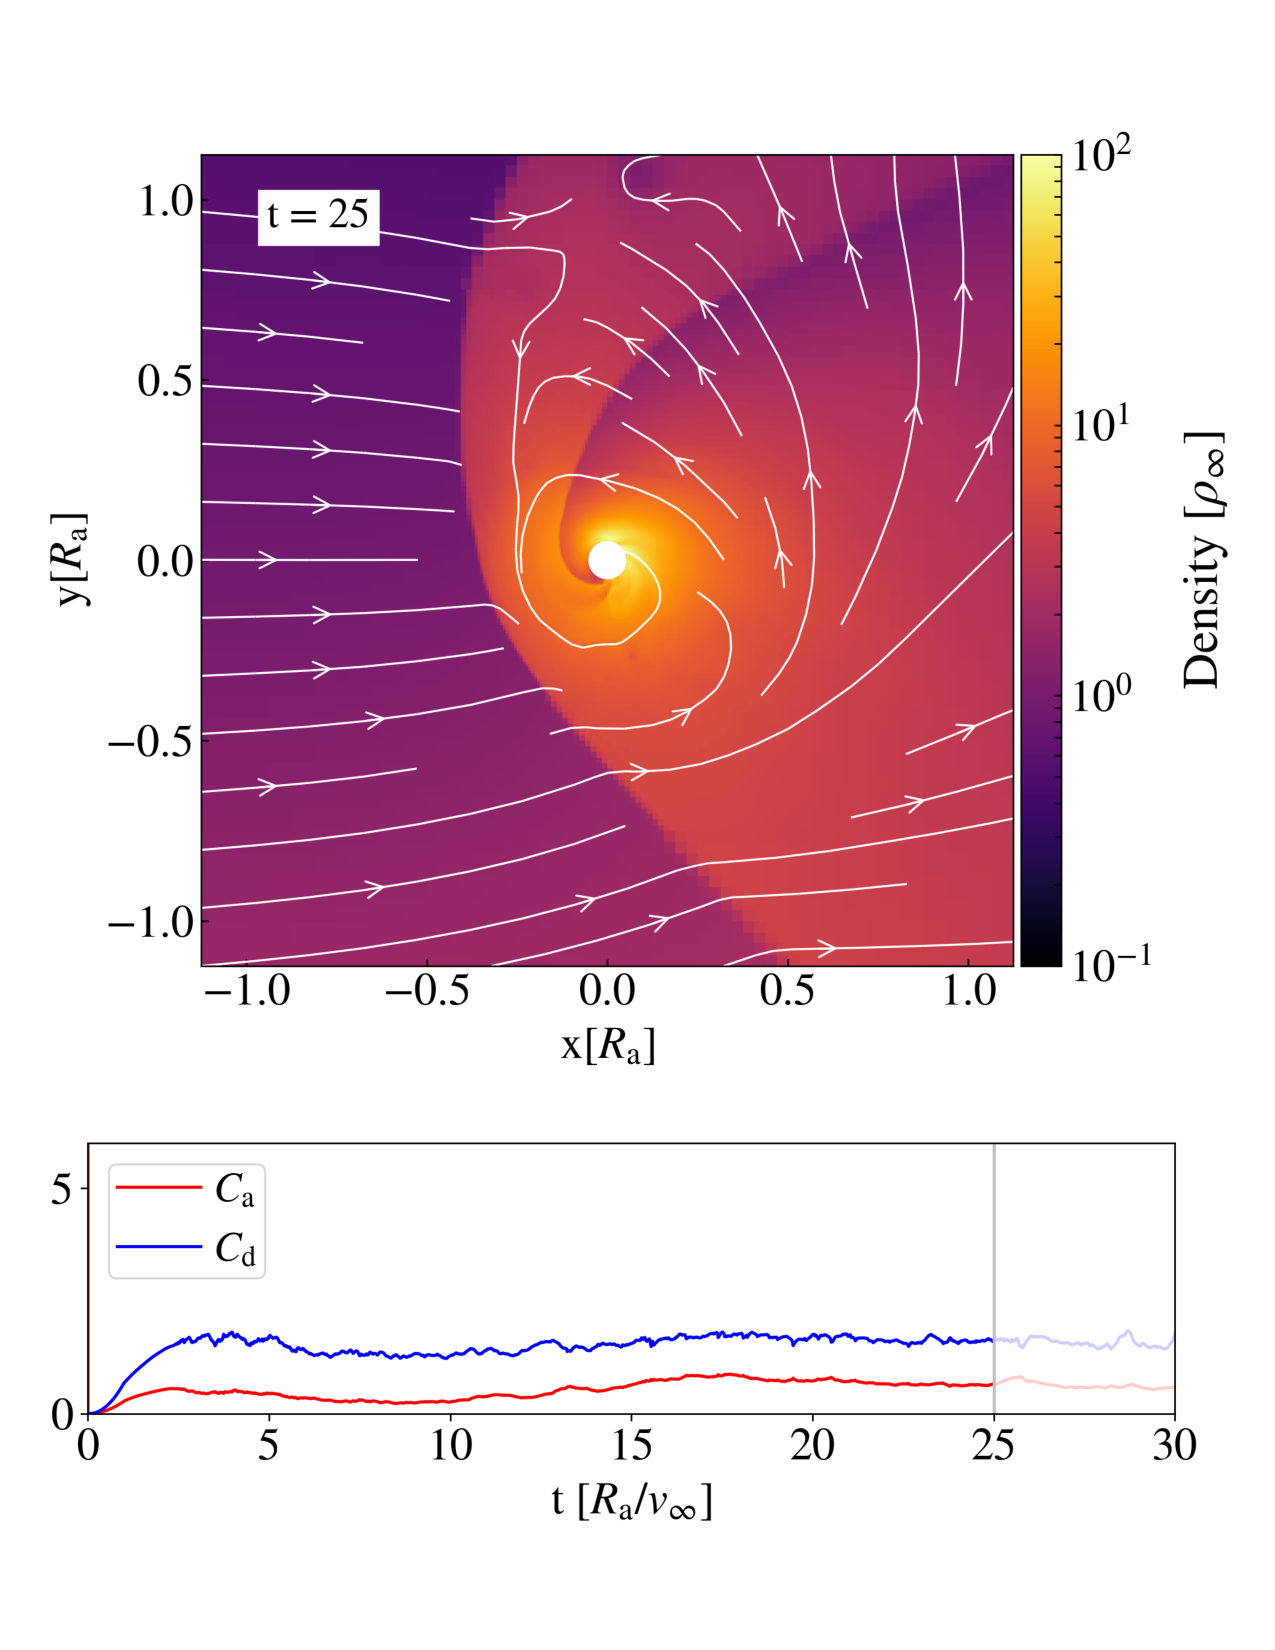
\includegraphics[width=10.5cm]{figures/common_envelope/movie_plot.pdf}
 \caption{Movie of a simulation showing flow of material in the vicinity of an object, embedded in the envelope of its companion star during a common envelope interaction. The simulation has been performed with ideal gas equation of state adiabatic constant $\gamma = 4/3$, mass ratio $q_{\rm r} = 0.1$, and upstream Mach number $\mathcal{M}_\infty = 1.69$ in the ``wind tunnel'' setup. The top panel shows the density in units of $\rho_\infty$ in the orbital ($x$-$y$) plane of the binary, with the white dot at the coordinate origin representing the embedded companion object. The lines with arrowheads in white represent streamlines following the velocity field in the flow. Material enters into the domain from the -x direction, and the coefficient of accretion $C_{\mathrm a}$, and the coefficient of drag $C_{\mathrm d}$ values are measured in response to the incoming conditions. Supersonic flow of material past the object results in a large pressure difference, causing formation of a shock wave. The bottom panel shows the time series of coefficients of accretion $C_{\mathrm a}$ (in red) and drag $C_{\mathrm d}$ (blue) for the full simulation. The gray vertical line tracks the instantaneous $C_{\mathrm a}$, $C_{\mathrm d}$ values as the simulation progresses. The time quoted in the movie is in code units $R_{\mathrm{a}}/v_\infty$, where $R_{\rm a}$ is the accretion radius and $v_\infty$ is the relative velocity of the flow past the embedded object. \label{fig:video_sim}}  %The bottom panel tracks the evolution of the coefficients of accretion $C_{\mathrm a}$ and drag $C_{\mathrm d}$ as a function of time.
\vspace*{5mm}
\end{figure}

\vspace*{2.5mm}
\subsection{Gas Flow}\label{sec:hydro}
In this section, we discuss the properties and morphology of gas flow in our Common Envelope Wind Tunnel experiments for the models tabulated in Tables \ref{tab:sims_43_params} and \ref{tab:sims_53_params}. We focus, in particular, on the differences that arise as we vary the dimensionless characteristics of the flow in the form of upstream Mach number, mass ratio, and gas adiabatic index. 

\subsubsection{Dependence on Mach Number, ${\cal M}_\infty$}\label{sec:hydro_mach}

\begin{figure*}[t]%[tbp]
\centering
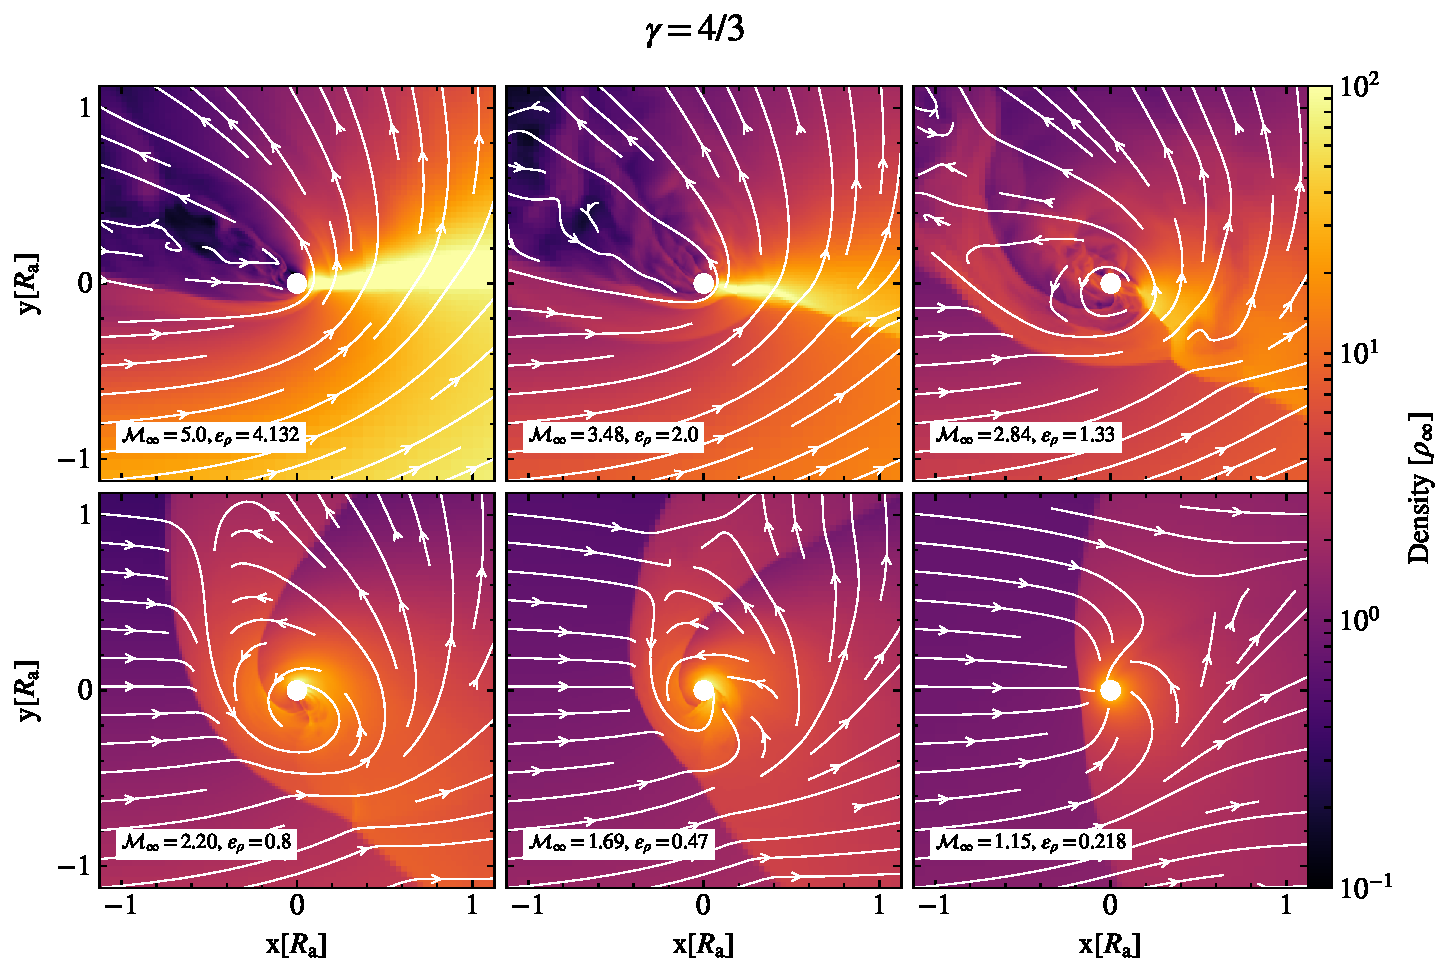
\includegraphics[width=13.8cm]{figures/common_envelope/sliceplot_gamma_43_q0pt1_varymach_gradient_comparison_figure_z.pdf}
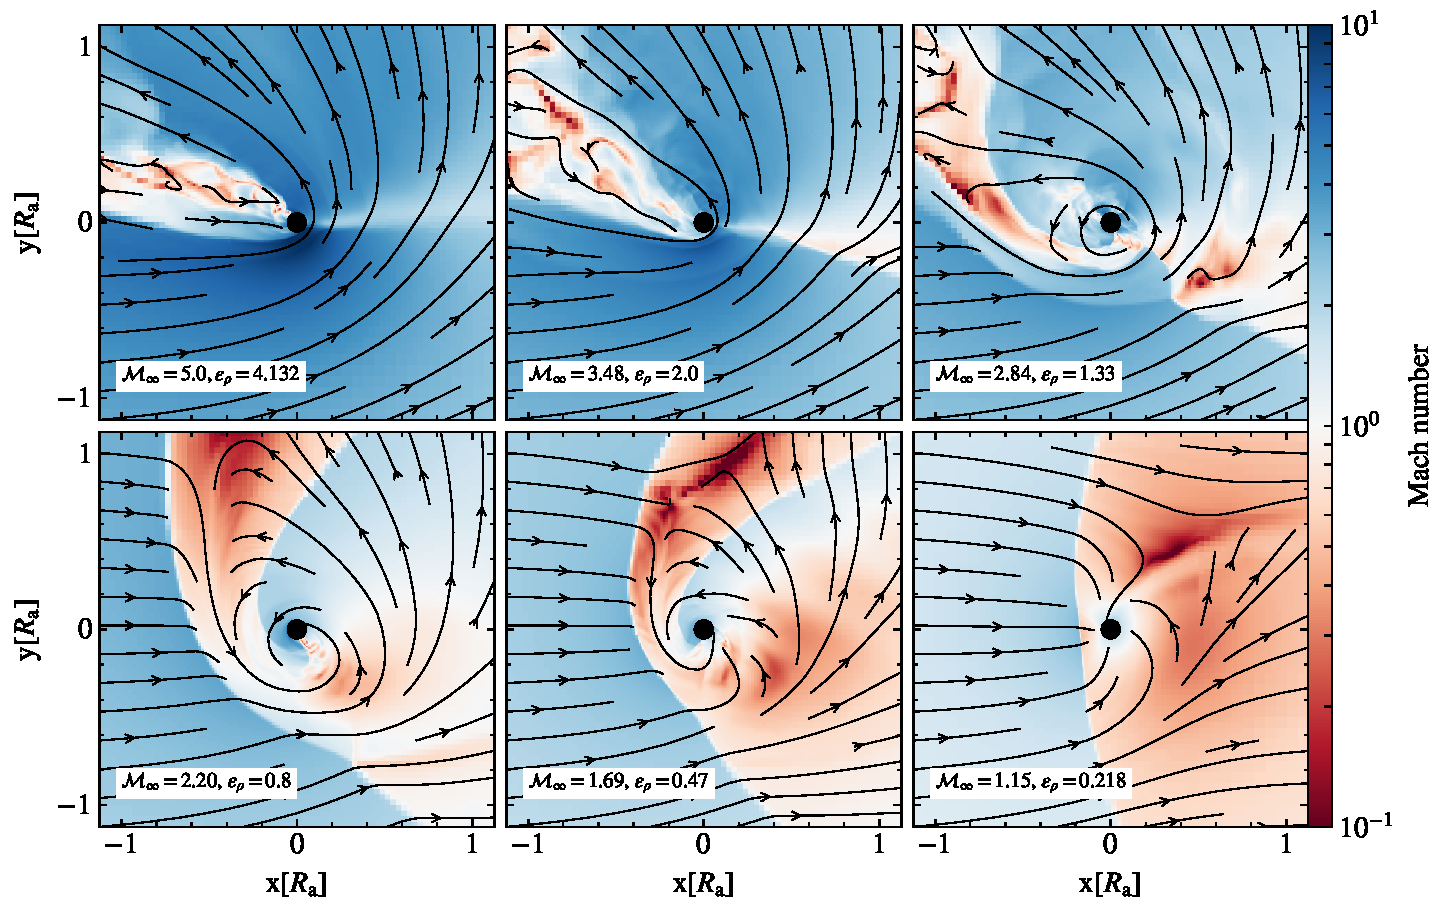
\includegraphics[width=13.8cm]{figures/common_envelope/sliceplot_gamma_43_q0pt1_varymach_mach_gradient_comparison_figure_z.pdf}
\caption{Slices of density in units of $\rho_\infty$ (upper panels) and Mach number (lower panels) through the orbital ($x$-$y$) plane, for a fixed mass ratio $q_{\rm r}$ and varying upstream Mach number $\mathcal{M}_\infty$, for the simulation suite $(\Gamma_{\rm s}, \gamma) = (4/3, 4/3)$. The simulations use $q_{\rm r} = 0.1$ and $\mathcal{M}_\infty$ 5.0, 3.48, 2.84, 2.20, 1.69, and 1.15 corresponding to density gradients $\epsilon_\rho$ of 4.132, 2.0, 1.33, 0.8, 0.47, and 0.218 respectively. The slices compare the state of the flow at simulation time $t = 30~R_{\mathrm{a}}/v_\infty$. Moving from the highest to the lowest $\mathcal{M}_\infty$, the slices show the pattern of the flow around the embedded companion object as it inspirals from the outer to the inner regions of the primary star's envelope.  
\label{fig:sims_g43_fix_q_vary_mach}}
\end{figure*}

\begin{figure*}[t]
\centering
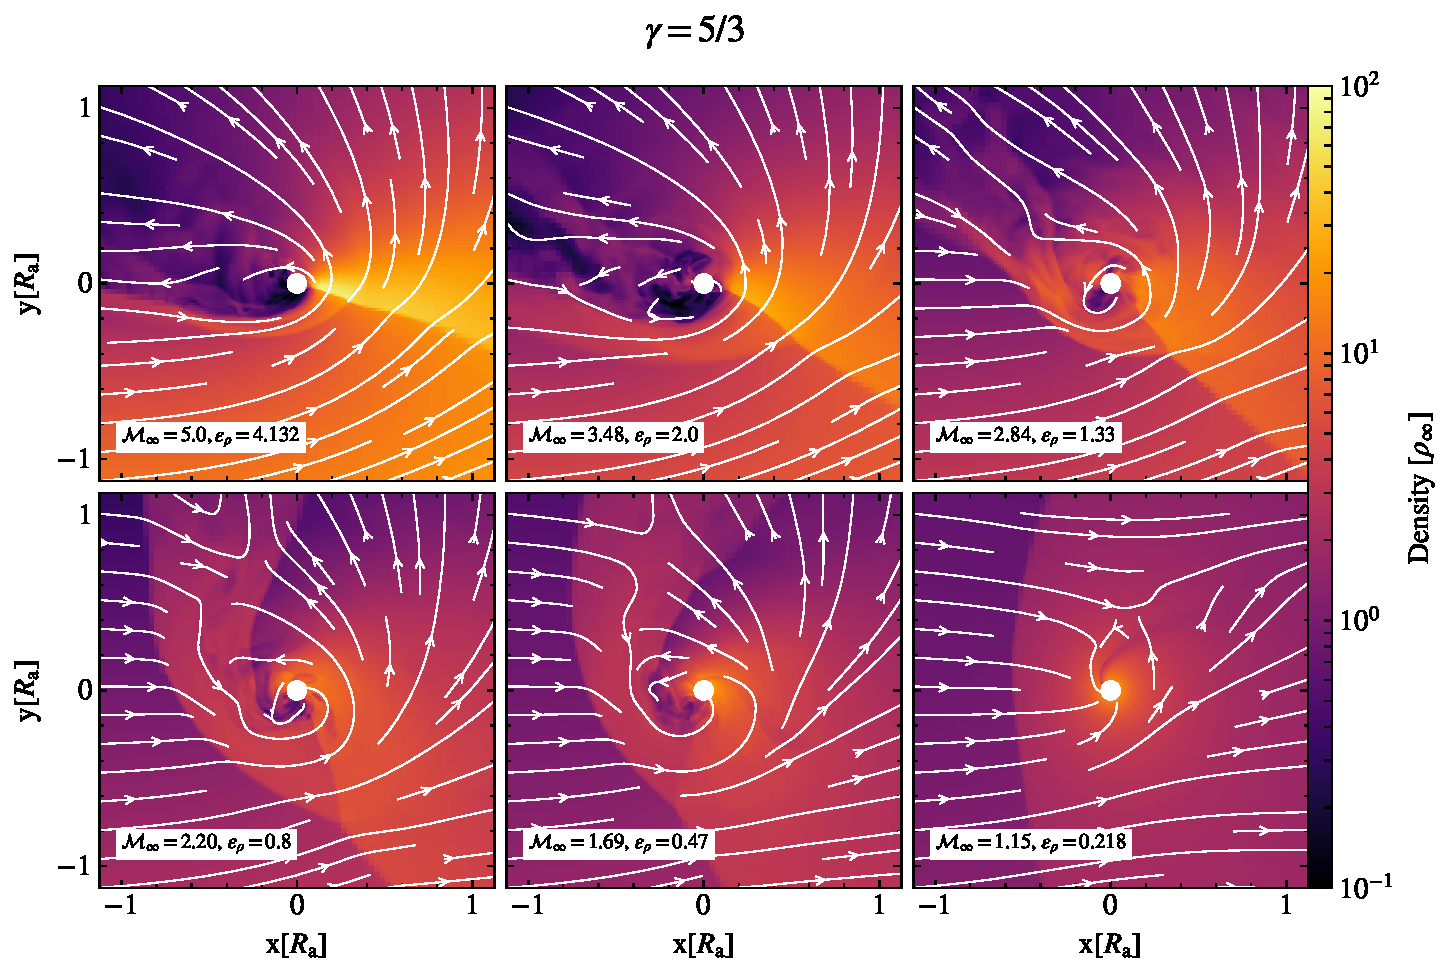
\includegraphics[width=13.8cm]{figures/common_envelope/sliceplot_gamma_53_q0pt1_varymach_gradient_comparison_figure_z.pdf}
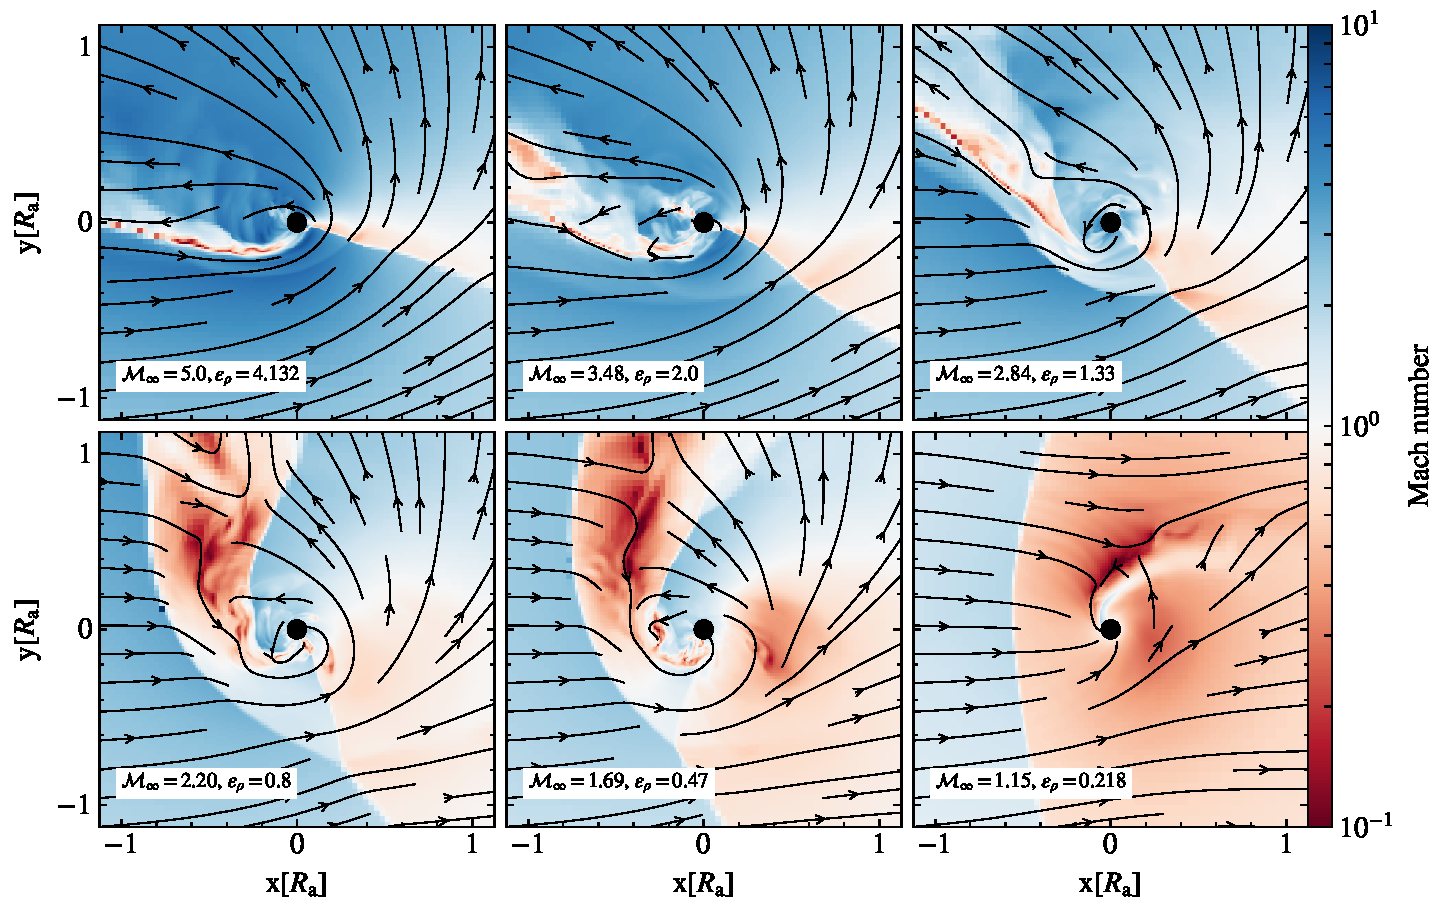
\includegraphics[width=13.8cm]{figures/common_envelope/sliceplot_gamma_53_q0pt1_varymach_mach_gradient_comparison_figure_z.pdf}
\caption{Slices of density in units of $\rho_\infty$ (upper panels) and Mach number (lower panels) through the orbital ($x$-$y$) plane, for a fixed mass ratio $q_{\rm r}$ and varying upstream Mach number $\mathcal{M}_\infty$, for the simulation suite $(\Gamma_{\mathrm s}, \gamma) = (5/3, 5/3)$. The simulations use $q_{\rm r} = 0.1$ and $\mathcal{M}_\infty$ 5.0, 3.48, 2.84, 2.20, 1.69, and 1.15 corresponding to density gradients $\epsilon_\rho$ of 4.132, 2.0, 1.33, 0.8, 0.47, and 0.218 respectively. The slices compare the state of the flow at simulation time $t = 30~R_{\mathrm{a}}/v_\infty$. Moving from the highest to the lowest $\mathcal{M}_\infty$, the slices show the pattern of the flow around the embedded companion object as it inspirals from the outer to the inner regions of the primary star's envelope. \label{fig:sims_g53_fix_q_vary_mach}}
\end{figure*}

Figures \ref{fig:sims_g43_fix_q_vary_mach} and \ref{fig:sims_g53_fix_q_vary_mach} show slices of density and Mach number through the orbital ($x$-$y$) plane from the models with $q_{\rm r} = 1/10$ and a range of $\mathcal{M}_\infty$ and corresponding $\epsilon_\rho$ values. In Figure \ref{fig:sims_g43_fix_q_vary_mach} models from Table \ref{tab:sims_43_params} are presented, which have $\gamma = \Gamma_{\mathrm s} = 4/3$, while in Figure \ref{fig:sims_g53_fix_q_vary_mach} models from Table \ref{tab:sims_53_params} are presented, which have $\gamma = \Gamma_{\mathrm s} = 5/3$. In these slices, the $x$ and $y$ axes show distances in units of the accretion radius $R_{\mathrm{a}}$, and we overplot streamlines of the velocity field within the $x$-$y$ plane. 


Higher Mach numbers imply steeper density gradients relative to the accretion radius, following equation \eqref{eq:mach-erho}.  These conditions tend to be found in the outer regions of the stellar envelope, whereas lower Mach numbers and shallower density gradients are more representative of flows found deeper in the stellar envelope. Thus, the sequence of Mach numbers approximates the inspiral of an object from the outer regions of the envelope of the donor star toward its center.


Figures \ref{fig:sims_g43_fix_q_vary_mach} and \ref{fig:sims_g53_fix_q_vary_mach} demonstrate how a decreasing $\mathcal{M}_\infty$ for fixed $q_{\rm r}$ affects the flow characteristics. A key distinction is that the flow symmetry is more dramatically broken at high $\mathcal{M}_\infty$ (and $\epsilon_{\rho}$), and it gradually becomes more symmetric with decreasing $\mathcal{M}_\infty$ and $\epsilon_{\rho}$ \cite{MacLeod_2015,MacLeod:2017}. It is important to emphasize that the controlling parameter generating this asymmetric flow is the density gradient, rather than the Mach number itself. In the highly asymmetric cases, the dense material from negative $y$ values does not stagnate at $y=0$, as in the canonical HL flow. Instead, this material pushes its way to positive $y$ values (where the background density is lower) as it is deflected by the gravitational influence of $M_2$. In the cases where  $\mathcal{M}_\infty = 1.15$, the flow is nearly symmetric as density gradients are quite mild and the flow morphology approaches that of the classic HL case.


The lower panels in Figures \ref{fig:sims_g43_fix_q_vary_mach} and \ref{fig:sims_g53_fix_q_vary_mach} show slices of flow Mach number near the embedded object. In case of the high upstream Mach numbers or steeper upstream density gradients, most of the material in the post-shock region is supersonic, with a negligible amount of material having $\mathcal{M} \ll 1$ values. As the upstream Mach number is decreased, or the upstream density gradient is made shallower, the bow shock becomes more symmetric. The upstream flow is supersonic, whereas after the material crosses the shock and meets the pressure gradient caused by the convergence of the flow in the post-shock region, the downstream flow becomes subsonic. %In Figure \ref{fig:sims_g43_fix_q_vary_mach}, we observe that material re-crosses a sonic surface as it falls inward toward the sink; due to the difference in adiabatic index, this feature is not present in the $\gamma=5/3$ models of Figure \ref{fig:sims_g53_fix_q_vary_mach}.
In Figure \ref{fig:sims_g43_fix_q_vary_mach}, for the lowest upstream Mach number case in the $\gamma = 4/3$ simulations, we observe a sonic surface in the Mach number plot, crossed by red post-shock material, as it transitions to blue (supersonic) infall towards the sink. For the $\gamma=5/3$ simulations, this feature is not visible, as the sonic point is located at the accretor (at zero radius).


We can anticipate the implications of these flow distributions on coefficients of accretion and drag. With increasing $\mathcal{M}_\infty$, the disturbance in the flow symmetry is expected to reduce the rate of accretion: streamlines show less material is converging toward the embedded object.  We also note that for larger density gradients (higher $\mathcal{M}_\infty$) the post-shock flow is generally more turbulent, and the rate of accretion of material into the sink becomes more variable. The variation of density flowing within the accretion radius in the high $\mathcal{M}_\infty$ cases lead dense material from negative $y$ regions to be focused into the object's wake, which might be expected to enhance the dynamical friction drag force.

\subsubsection{Dependence on Mass Ratio, $q_{\rm r}$}\label{sec:hydro_q}

\begin{figure*}
\centering
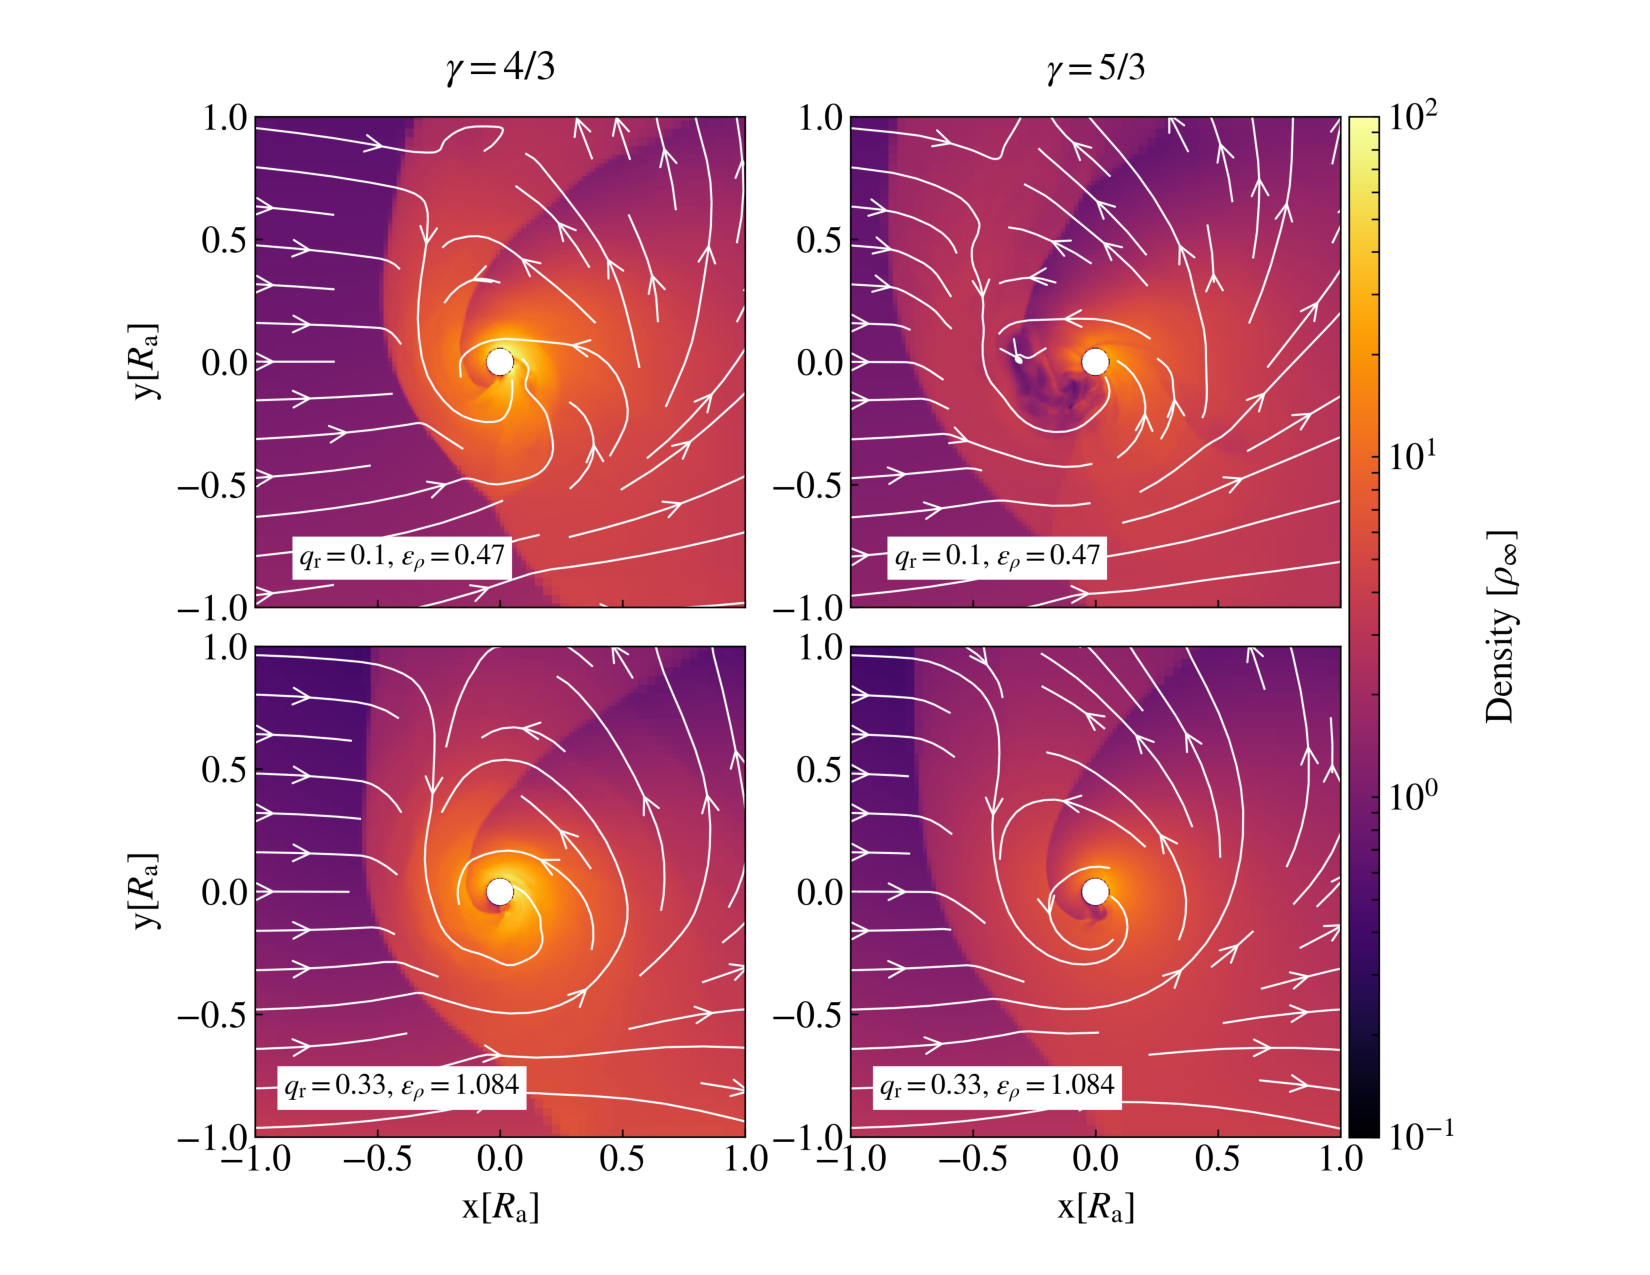
\includegraphics[width=16cm]{figures/common_envelope/sliceplot_gamma_43_53_mach1pt69_varyq_gradient_comparison_figure_z.pdf}
\caption{Slices of density in units of $\rho_\infty$ for the simulation suite $(\Gamma_s, \gamma) = (4/3, 4/3)$ (left panels) and for the simulation suite $(\Gamma_s, \gamma) = (5/3, 5/3)$ (right panels) through the orbital ($x$-$y$) plane, for a fixed upstream Mach number $\mathcal{M}_\infty$ and varying ratio $q_{\rm r}$. The simulations for each $\gamma$ use $\mathcal{M}_\infty = 1.69$ and $q_{\rm r}=0.1$ (top) and 0.33 (bottom). The slices compare the state of the flow at simulation time $t = 30~R_{\mathrm{a}}/v_\infty$. The panels show the dependence of the flow pattern around the embedded companion object in a specific region of the envelope on the binary mass ratio. \label{fig:sims_fix_mach_vary_q}}
\vspace*{8mm}
\end{figure*}

Varying mass ratio can be representative of differing binary initial conditions, or even changing enclosed mass within a given binary.  
Figure~\ref{fig:sims_fix_mach_vary_q} shows slices of density  through the orbital ($x$-$y$) plane from the simulations performed for $q_{\rm r}$ values $1/10$ and $1/3$ and a fixed $\mathcal{M}_\infty = 1.69$ for both $\gamma=\Gamma_{\mathrm s}=4/3$ and $\gamma=\Gamma_{\mathrm s}=5/3$.


Comparison of the panels of Figure~\ref{fig:sims_fix_mach_vary_q} demonstrates the effect of $q_{\rm r}$ on the flow characteristics. 
Although $\mathcal{M}_\infty$ is held constant, the corresponding $\epsilon_\rho$ is largest in the $q_{\rm r} = 1/3$ case, and smallest for $q_{\rm r} = 1/10$, as shown in Tables \ref{tab:sims_43_params} and \ref{tab:sims_53_params}. This yields the most obvious difference with varying $q_{\rm r}$: the flow in the $q_{\rm r}=1/3$ case is more asymmetric (for example the bow shock is more distorted) as a result of the stronger density gradient. Secondly, we observe that the higher $q_{\rm r}$ cases have weaker focusing of the flow around the embedded object, as evidenced by the pre-shock flow streamlines. This happens because as the mass ratio increases, from equation~\eqref{eq:Ra_asfunc_a}, $R_{\mathrm a}/a$ increases. We choose our model domain sizes to capture this difference in scales, as described in Section \ref{sec:method}. When the accretion radius is a larger fraction of the orbit size, gravitational focusing acts over fewer characteristic lengths $R_{\rm a}$ to concentrate the flow. One implication is that the effective interaction cross section is smaller than $\pi R_{\mathrm{a}}^2$, because the original HL derivation of $R_{\mathrm{a}}$ assumes a ballistic trajectory focused from infinite distance. 

Therefore, with increasing $q_{\rm r}$, we anticipate a decrease in the dynamical friction drag force due to the smaller effective cross section. The implications for the accreted mass are less obvious from these slices because the morphology of the post-shock flow is largely similar due to the competition between steeper density gradients but smaller effective cross sections at larger $q_{\rm r}$. 

\subsubsection{Dependence on Adiabatic Index, $\gamma$}\label{sec:hydro_gamma}

Here we examine the dependence of flow properties on the stellar envelope equation of state, using two limiting cases of ideal-gas equations of state that bracket the range of typical stellar envelope conditions. 
A $\gamma=4/3$ equation of state is representative of a radiation pressure dominated equation of state, occuring in massive-star envelopes, or in zones of partial ionization in lower-mass stars. A $\gamma=5/3$ equation of state represents a gas-pressure dominated equation of state, as occurs in the interiors of relatively low-mass stars with masses less than approximately $ 8 M_\odot$ (e.g., \cite{MacLeod:2017,Murguia-Berthier:2017}). Values between these limits are also possible, dependent on the microphysics of the density--temperature regime \cite{Murguia-Berthier:2017}.

While there are many similarities in overall flow morphology in our simulation suites A (Table \ref{tab:sims_43_params}) and B (Table \ref{tab:sims_53_params}), because gas is less compressible with $\gamma=5/3$ than it is with $\gamma=4/3$, there are a several key differences between these two cases.   Gas near the accretor tracks closer to ballistic, rotationally-supported trajectories in the $\gamma = 4/3$ case, as compared to the less compressible $\gamma = 5/3$ case. A related feature is that the bow shock stands further off from the accretor into the upstream flow when  $\gamma = 5/3$  than $\gamma=4/3$. These properties are visible when comparing the equivalent panels of Figure~\ref{fig:sims_g53_fix_q_vary_mach} and Figure~\ref{fig:sims_g43_fix_q_vary_mach}, or the left and right panels of Figure~\ref{fig:sims_fix_mach_vary_q}.  The underlying explanation is similar, shock structures around the accretor are set by the balance of the gravitational attraction of the accretor, the ram pressure of incoming material, and pressure gradients that arise as gas is gravitationally focused.  For the less-compressible $\gamma=5/3$ models, gas pressure gradients exceed the accretor's gravity, and partially prevent accretion. We observe the consequence of this in lower-density voids of hot, low Mach number material in Figure \ref{fig:sims_g53_fix_q_vary_mach}. For the more compressible $\gamma = 4/3$ flow, gas is more readily compressed, and pressure gradients build at a similar rate to the gravitational force \cite{Murguia-Berthier:2017}. One consequence of this is that higher densities near the accretor track the compression of gas deep into the accretor's gravitational potential well.

\vspace{2.5mm}
\subsection{Coefficients of Drag and Accretion}\label{sec:coeff}

We now use the results from the wind tunnel experiments to understand the effects of $q_{\rm r}$ and $\mathcal{M}_\infty$ on the accretion of material onto the embedded object and on the drag force acting on the embedded object. 
Figure~\ref{fig:datapoints_Ca_Cd_vs_mach_g43_g53_sims} shows median values of $C_{\mathrm a}$ and $C_{\mathrm d}$ computed over simulation times $10~R_{\mathrm{a}}/v_\infty < t < 30~R_{\mathrm{a}}/v_\infty$, as a function of $\mathcal{M}_\infty$ for different values of $q_{\rm r}$. We use contributions from both the dynamical friction drag force, $F_{\rm{df}}$, and the force due to linear momentum accretion $F_{\dot p_x}$ in calculating $C_{\rm d}$ (Equation \ref{eq:C_d}). In all our simulations, $F_{\rm{df}}$ is larger than $F_{\dot p_x}$, however, as we find in Section \ref{sec:sink}, the sum of these forces is the quantity that is invariant with respect to changing the numerical parameter of sink radius.

In Appendix \ref{subsec:fits}, we present fitting formulae for the coefficients of accretion $C_{\mathrm a}$ and drag force $C_{\mathrm d}$ as a function of the mass ratio and Mach number from both our $\gamma = 4/3$ and $\gamma = 5/3$ simulations, showing the mapping between the $(q_{\rm r}, \mathcal{M}_\infty) \rightarrow (C_{\mathrm a}, C_{\mathrm d})$ parameter space that we have explored. 



\begin{figure*}
  \centering
  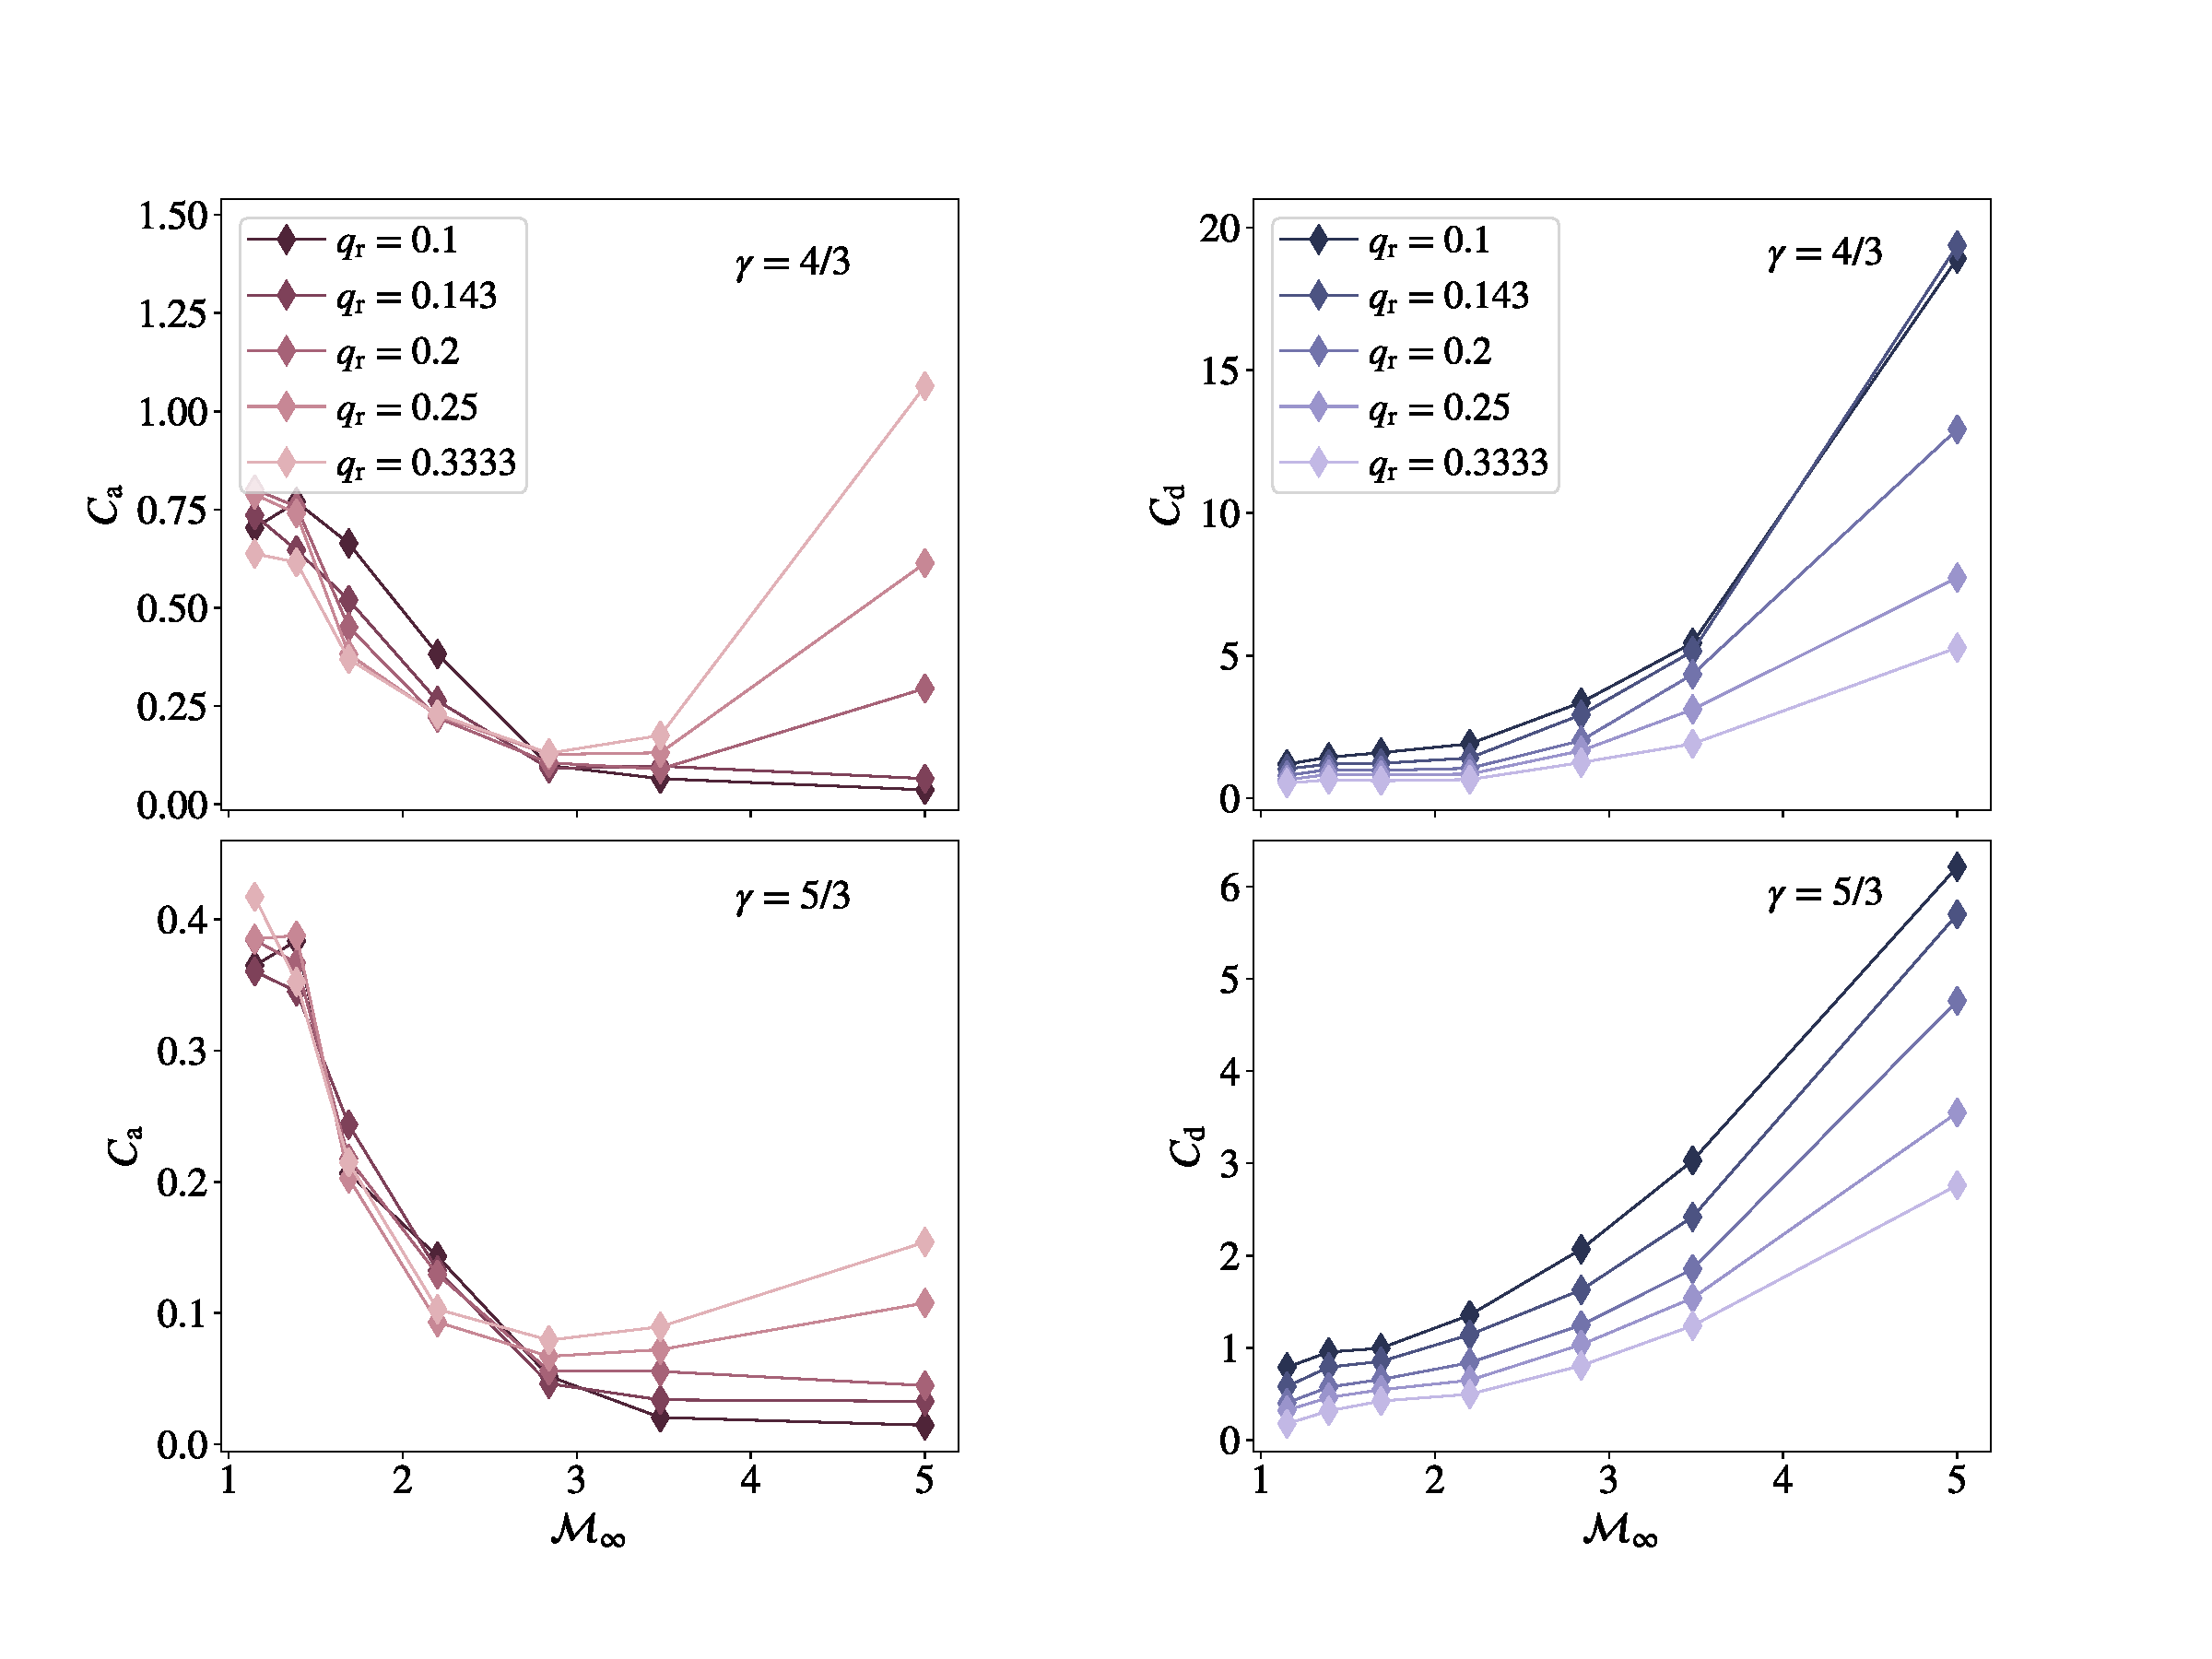
\includegraphics[width=\textwidth]{figures/common_envelope/gamma_43_53_Ca_Cd_vs_mach_q_comparison_inc_mdotdrag.pdf}
  \caption{Variations of the median coefficient of accretion $C_{\mathrm a}$ and the median coefficient of drag $C_{\mathrm d}$ versus upstream Mach number $\mathcal{M}_\infty$ for the $(\Gamma_s, \gamma) = (4/3, 4/3)$ simulations (top panels) and $(\Gamma_s, \gamma) = (5/3, 5/3)$ simulations (bottom panels). $C_{\mathrm a} (C_{\mathrm d})$ vs. $~\mathcal{M}_\infty$ curves are shown for each $q_{\rm r}$ value at which simulations are performed. $C_{\mathrm a}$ is obtained by normalizing the mass accretion rate in the system to the HL theory mass accretion rate. $C_{\mathrm d}$ is obtained by normalizing the drag force in the system to the HL theory drag force. The $C_{\mathrm a}$ and $C_{\mathrm d}$ median values are computed in the simulation time range $10~R_{\mathrm{a}}/v_\infty < t < 30~R_{\mathrm{a}}/v_\infty$. For a fixed, small mass ratio $q_{\rm r}$, a higher $\mathcal{M_\infty}$ corresponds to a steeper upstream density gradient which breaks the symmetry of the flow, causing a reduction in $C_{\mathrm a}$; and a greater quantity of dense material gravitationally focused from the deep stellar interior, which increases $C_{\rm d}$. \label{fig:datapoints_Ca_Cd_vs_mach_g43_g53_sims}}
\vspace*{1cm}
\end{figure*}

\subsubsection{Dependence on Mach Number, ${\cal M}_\infty$}\label{sec:coeff_mach}

We begin by examining the dependence of drag and accretion coefficients with upstream Mach number, ${\cal M}_\infty$. 
Figure~\ref{fig:datapoints_Ca_Cd_vs_mach_g43_g53_sims} shows that for ${\cal M}_\infty \lesssim 3$, at fixed $q_{\rm r}$, $C_{\rm a}$ decreases with increasing $\mathcal{M}_\infty$. For $q_{\rm r}\lesssim0.2$, this trend continues to higher $\mathcal{M}_\infty$, while for $q_{\rm r} \gtrsim 0.2$, the coefficient of accretion rises again with increasing $\mathcal{M}_\infty$, particularly in the $\gamma=4/3$ models. This general trend can be understood in the context of the associated density gradients. For fixed $q_{\rm r}$, higher $\mathcal{M}_\infty$ flows correspond to steeper density gradients relative to the accretion radius. The steep density gradient breaks the symmetry of the post-shock flow, as discussed in Section \ref{sec:hydro_mach}. The resulting net rotation and  angular momentum act as a barrier to accretion, and lead to a drop in the accretion rate as compared to the HL rate ($\pi R_{\mathrm{a}}^2 \rho_\infty v_\infty$) \cite{MacLeod_2015}. The increase in $C_{\rm a}$ for large $q_{\rm r}$ at high $\mathcal{M}_\infty$  runs counter to this overall trend. In these cases, the combined steepening of the density gradient and weakening of the overall gravitational focus and slingshot discussed in Section \ref{sec:hydro_q} leads to a flow morphology that very effectively transports dense material from $-y$ impact parameters toward the sink, instead of imparting so much angular momentum that it is flung to $+y$ coordinates, resulting in large $C_{\rm a}$.

As for the drag force, we see that for each value of $q_{\rm r}$, $C_{\mathrm d}$ monotonically increases by a factor of $\mathcal{O}(10)$ with increasing $\mathcal{M}_\infty$ across the range of $\mathcal{M}_\infty$ values for which we have performed simulations. This trend reflects the fact that higher local gas densities, $\rho$, are achieved within the accretion radius of $M_2$ for higher values of the upstream Mach number, $\mathcal{M}_\infty$. This higher density material ($\rho \gg \rho_\infty$) focused into the wake of the embedded object from deeper inside the interior of the primary star enhances the dynamical friction drag force as compared to the HL drag force ($\pi R_{\mathrm{a}}^2 \rho_\infty v_\infty^2$).


\subsubsection{Dependence on Mass Ratio, $q_{\rm r}$}\label{sec:coeff_q}

For each $\mathcal{M}_\infty$, we can also see the dependence of $C_{\rm a}$ and $C_{\rm d}$ on the mass ratio $q_{\rm r}$ in Figure~\ref{fig:datapoints_Ca_Cd_vs_mach_g43_g53_sims}. As the mass ratio increases, the accretion radius becomes a larger fraction of the orbit size. This causes the flows to be focused from a distance that is a smaller multiple of the accretion radius, causing weaker focusing and gravitational slingshot of the gas, as discussed in Section \ref{sec:hydro_q}. The effect of this difference on the coefficients of accretion at $\cal{M}_\infty \lesssim$ 3 is minimal. However, as discussed above in Section \ref{sec:coeff_mach},  at higher $\cal{M}_\infty$, there is a dramatic increase in $C_{\rm a}$ with increasing $q_{\rm r}$ that results in the capture of dense material from $-y$ impact parameters that does not possess sufficient momentum to escape the accretor's gravity. 

%The counterpoint of weakened momentum transfer to the gas in the higher $q_{\rm r}$ cases is that the embedded object is impeded less by this gravitational interaction.
In the higher $q_{\rm r}$ cases, there is relatively weak momentum transfer to the gas. This weakens the drag forces relative to the HL drag force, which reduces the deceleration of the object. In section \ref{sec:hydro_q}, we discussed this effect in terms of a reduced effective cross section. In terms of the coefficients of drag in Figure~\ref{fig:datapoints_Ca_Cd_vs_mach_g43_g53_sims}, the quantitative effects are particularly clear. When gas is gravitationally focused over fewer characteristic length scales (because $R_{\rm a}$ is a larger fraction of $a$ at larger $q_{\rm r}$) we see lower dimensionless drag forces, $C_{\rm d}$. 

\subsubsection{Dependence on Adiabatic Index, $\gamma$}\label{sec:coeff_gamma}

The gas adiabatic index has important consequences for coefficients of drag and accretion because while pressure gradients enter into the fluid momentum equation, distributions of gas densities set rates of drag and accretion. Thus, the equation of state is crucial for both the flow morphology, as discussed in Section \ref{sec:hydro_gamma}, and for $C_{\rm a}$ and $C_{\rm d}$.

In Figure~\ref{fig:datapoints_Ca_Cd_vs_mach_g43_g53_sims} we note that the increased resistance to compression by the accretor's gravitational force of the $\gamma = 5/3$ models leads to lower $C_{\rm a}$ by a factor of approximately 2 than the equivalent $\gamma=4/3$ models.   We saw the effects of this in the density slices of Figures \ref{fig:sims_g43_fix_q_vary_mach} and \ref{fig:sims_g53_fix_q_vary_mach}, in which the material in the vicinity of $M_2$ is not as dense in the $\gamma = 5/3$ models as it is in the $\gamma = 4/3$ simulations.  Second, the larger pressure support provided by the gas in the $\gamma = 5/3$ simulations decreases the overdensity of the post-shock wake versus what is realized in the simulations with $\gamma = 4/3$.  The greater upstream-downstream symmetry that results, decreases the net dynamical friction force exerted on the embedded object. We observe that $C_{\rm d}$ is approximately a factor of 3 lower for $\gamma=5/3$ than $\gamma=4/3$ in the right panels of Figure~\ref{fig:datapoints_Ca_Cd_vs_mach_g43_g53_sims}. 

Having explored the parameter space of gas flow and coefficients of gas and accretion in our wind tunnel models, in the following section, we explore the application of these results to astrophysical common envelope encounters. In Appendix \ref{sec:compare_drag}, we compare the drag forces measured in this work with other approaches to measure drag forces in common envelope encounters.

\vspace{5mm}
\section{Accretion onto Black Holes During a Common Envelope Inspiral}\label{sec:implications}
In this section we discuss the application of our wind tunnel results to the scenario of a black hole dynamically inspiraling through the envelope of its companion. We focus in particular on the accreted mass and spin, because these parameters directly enter into the gravitational-wave observables.  To do so, we discuss the application and extrapolation of our numerical measurements of $C_{\rm a}$ and $C_{\rm d}$ to black holes, and the implications on the accreted mass and spin for LIGO-Virgo's growing binary black hole merger population. 

\vspace*{2.5mm}
\subsection{Projected Accretion and Drag Coefficients for Compact Objects}\label{sec:sink}

A limitation of our numerical models is that the accretion rate, and to a lesser extent the drag force, have been shown to depend on the size of the central absorbing sink (see \cite{1994ApJ...427..351R, 1994A&AS..106..505R,1995A&AS..113..133R, 2012ApJ...752...30B,MacLeod_2015,Antoni:2019pgq}). This dependence indicates that results do not converge to a single value regardless of the numerical choice of sink radius, $R_{\rm s}$. Further, simultaneously resolving the gravitational focusing radius, $R_{\rm a}$, and the size of a compact object is currently not computationally feasible: $R_{\rm a}$ might be on the order of the envelope radius, while an embedded compact object's radius is orders of magnitude smaller still. Previous work by Refs. \cite{MacLeod:2014yda,MacLeod_2015} and Ref. \cite{MacLeod:2017} has pointed out that these limitations make accretion coefficients derived from simulations at most upper limits on the realistic accretion rate. 

Here we attempt to systematically explore the scaling of coefficients of accretion and drag to smaller sink radii, that is smaller $R_{\rm s}/R_{\rm a}$. We ran two additional sets of 35 models that reproduce models A1 through A35, reducing the sink radius by a factor of two to $R_{\rm s}/R_{\rm a}=0.025$ and $R_{\rm s}/R_{\rm a}=0.0125$. To preserve the same level of resolution across the sink radius, we add an additional layer of mesh refinement around the sink with each reduction of sink radius (effectively halving the minimum zone width). From these models, we measure coefficients of drag and accretion following the methodology identical to our standard models presented earlier. 

With accretion and drag coefficients derived across a factor of four in sink radius, we fit the dependence on sink radius with power laws of the form 
\begin{equation}\label{eq:powerlawacc}
    \log_{\rm 10}\left( \dot M \right) = {\alpha_{\dot M}} \log_{\rm 10}\left( R_{\rm s}/R_{\rm a} \right) + {\beta_{\dot M}}
\end{equation}
\begin{equation}\label{eq:powerlawdrag}
    \log_{\rm 10}\left( F_{\rm d} \right) = {\alpha_{\rm F}} \log_{\rm 10}\left( R_{\rm s}/R_{\rm a} \right) + {\beta_{\rm F}}.
\end{equation}
Thus $\dot M \propto \left(R_{\rm s}/R_{\rm a}\right)^{\alpha_{\dot M}}$ and $F_{\rm d} \propto \left(R_{\rm s}/R_{\rm a}\right)^{\alpha_{\rm F}}$. With these coefficients, we have some indication of how rates of accretion and drag forces might extrapolate to much smaller $R_{\rm s}/R_{\rm a}$ that are astrophysically realistic. 

\begin{figure}[tbp]
\centering
 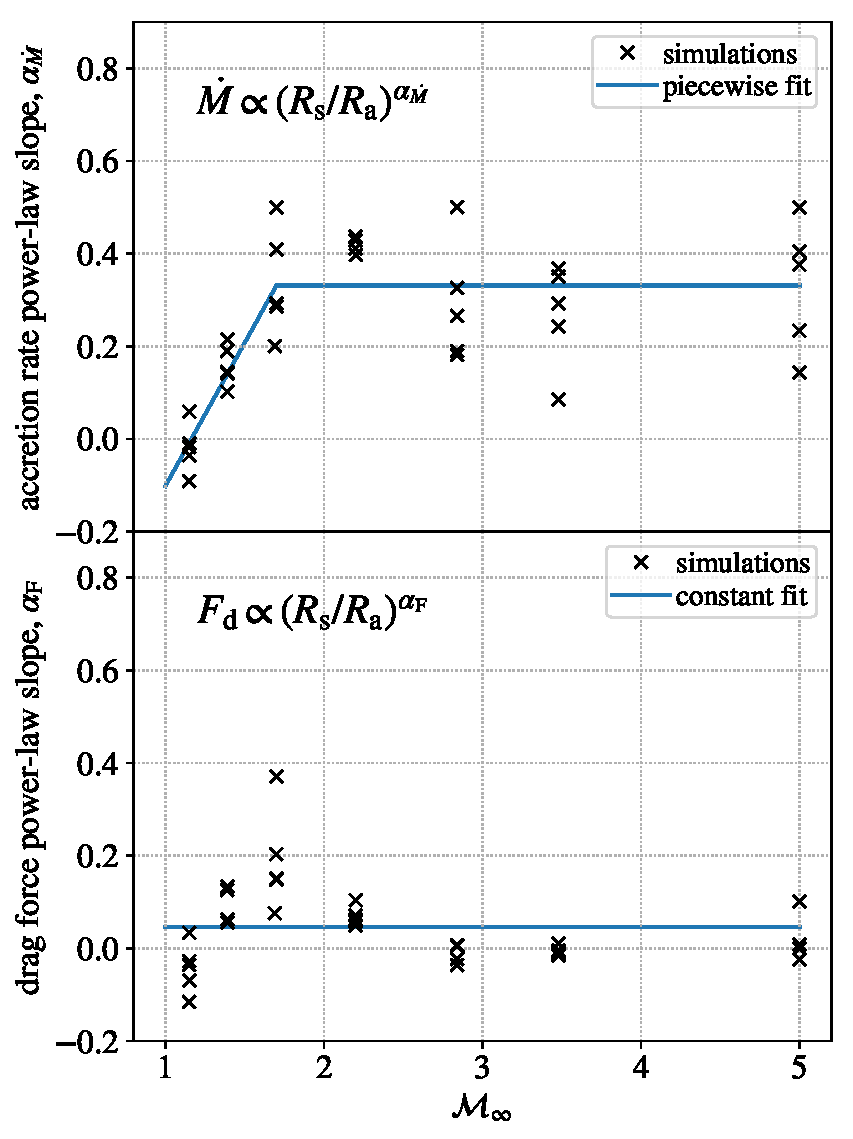
\includegraphics[width=10.5cm]{figures/common_envelope/Sink_Scaling.pdf}
 \caption{The figure shows exponents of power-law relations of the accretion rate, $\alpha_{\dot M}$, and drag force, $\alpha_{\rm F}$, on the sink radius. Top panel: For each $\gamma = 4/3$ simulation in Table~\ref{tab:sims_43_params}, an $\alpha_{\dot M}$ (denoted by a cross marker) is derived from a linear least-squares fit of Eq.~\eqref{eq:powerlawacc} to the $C_{\rm a}$ value measured from that simulation of sink size $R_{\rm s} = 0.05~R_{\rm a}$, plus similar simulations with $R_{\rm s} = [0.025, 0.0125]~R_{\rm a}$. The plot shows a largely-positive $\alpha_{\dot M}$, which indicates that accretion rates decrease as sink size decreases. The blue line shows a fit to the dependence of $\alpha_{\dot M}$ on $\cal {M}_\infty$, using the piecewise fitting relation given by Eq.~\eqref{eq:piecewise}.
 Lower panel: Following the same procedure for calculating $\alpha_{\dot M}$, each $\alpha_{\rm F}$ (denoted by a cross marker) value is derived from a linear least-squares fit of Eq.~\eqref{eq:powerlawdrag} to $C_{\rm d}$ values from simulations of varying sink sizes. The plot shows values of $\alpha_{\rm F} \sim 0$, indicating little change in the overall drag force as the sink radius is modified. The blue line shows $\alpha_{\rm F}$ across $\cal {M}_\infty$ values using a constant least-squares fit, which gives $\alpha_{\rm F} \approx 0.05$.
 \label{fig:sink} }
\vspace{5mm}
\end{figure}


Figure \ref{fig:sink} presents the exponents of the power-law relations of the accretion rate and drag force on the sink radius, as a function of ${\cal M}_{\infty}$.  For each ($q_{\rm r}, \cal M_\infty$) model, there are three sets of ($C_{\rm a}, C_{\rm d}$) values from the $R_{\rm s}/R_{\rm a}$ = [0.0125, 0.025, 0.05] simulations respectively. A linear least-square fit of Eq.~\ref{eq:powerlawacc} to the three $C_{\rm a}$ values is performed. The slope of the fitted line is $\alpha_{\dot M}$, that is the exponent of the power law function relating $\dot M$ to $R_{\rm s}/R_{\rm a}$. Similarly, a linear least-square fit of Eq.~\ref{eq:powerlawdrag} to the three $C_{\rm d}$ values is used to derive $\alpha_{\rm F}$, the exponent of the power law function relating $F_{\rm d}$ to $R_{\rm s}/R_{\rm a}$. Thus, we derive one $\alpha_{\dot M}$ and one $\alpha_{\rm F}$ (represented with cross markers in Fig.~\ref{fig:sink}) per ($q_{\rm r}, \cal{M}_\infty$) model. We observe that the majority of the $\alpha_{\dot M}$ values are positive, indicating that accretion rates drop as sink sizes get smaller relative to $R_{\rm a}$. Additionally, we observe that $\alpha_{\dot M}$ is typically lower in low Mach number flows, ${\cal M}_\infty \lesssim 2$, which have proportionately shallower density gradients. Above  ${\cal M}_\infty \gtrsim 2$, $\alpha_{\dot M}$ is approximately constant with increasing ${\cal M}_\infty$. At a given ${\cal M}_\infty$, there is variation between the models, depending on the mass ratio, $q_{\rm r}$. However, for simplicity, the following piecewise linear plus constant least-squares fit (blue line in Figure \ref{fig:sink}) reproduces the main trends
\begin{equation}\label{eq:piecewise}
\alpha_{\dot M} \approx 
\begin{cases}
0.62 {\cal M}_\infty - 0.72,& \ \ {\cal M}_\infty < 1.7, \\
0.33,& \ \ {\cal M}_\infty \geq 1.7 .
\end{cases}
\end{equation}



By comparison, exponents of power-law dependence of the drag coefficients on sink radius, $\alpha_{\rm F}$, do not show particularly structured behavior with ${\cal M}_\infty$. Further, most values are near zero, with all but one model lying within $-0.2 < \alpha_{\rm F} < 0.2$. Least-squares fitting of a constant finds $\alpha_{\rm F} \approx 0.05$, that is close to 0. This indicates that there is little change in the drag force with changing sink size.

Taken together, these scalings indicate that when $R_{\rm s}/R_{\rm a} \ll 1$, we can expect drag forces to remain relatively unchanged while accretion rate decreases. As a specific example, if an accreting black hole has $R_{\rm s}/R_{\rm a}=10^{-5}$ at ${\cal M}_\infty=2$, our scaling above suggests that we can expect the realistic accretion coefficient to be approximately 6\% of the value derived in our simulations with $R_{\rm s}/R_{\rm a}=0.05$ (because $(10^{-5}/0.05)^{0.33}\approx 0.06$).  This result makes intuitive sense in light of our simulation results: drag forces arise from the overdensity on the scale of $R_{\rm a}$, while, especially in the higher ${\cal M}_{\infty}$ (higher $\epsilon_\rho$) cases, rotation inhibits radial, supersonic infall of gas to the smallest scales.  

\vspace*{2.5mm}
\subsection{Coupled Orbital Tightening and Accretion}\label{sec:coupled}
As a black hole spirals through the common envelope gas, its orbit tightens in response to drag forces, and it may also potentially accrete mass from its surroundings. Under the HL theory of mass accretion and drag, the degree of mass growth is coupled to the degree of orbital tightening. Thus, a given orbital transformation is always accompanied by a corresponding mass change in this theory. Refs. \cite{Chevalier:1993,Brown:1995,Bethe:1998} elaborated on this argument, and suggested that compact objects in common envelope phases might easily double their masses. 

Here we re-express this line of argument with the addition of separate coefficients of drag and accretion (which might, for example, be motivated by numerical simulations). Orbital energy, $E = -GM_1 M_2 / 2 a$, is dissipated by the drag force at a rate $\dot E = - F v$ (if force is defined positive, as in our notation). Expressed in terms of the coefficient of drag, $\dot E = - C_{\rm d} F_{\rm HL} v = - C_{\rm d} \dot M_{\rm HL} v^2 = - C_{\rm d} \dot E_{\rm HL}$ (equations \eqref{eq:mdotHL} and \eqref{eq:fHL}). We will approximate the relative velocity here as the Keplerian velocity, such that $v^2 \approx G(M_1 + M_2)/a$. We can then write the mass gain per unit orbital energy change,
\begin{align}
\frac{dM_2}{dE} &=\frac{\dot M}{\dot E} = - \frac{C_{\rm a} \dot M_{\rm HL} }{C_{\rm d} \dot M_{\rm HL} v^2} = - \frac{C_{\rm a}  }{C_{\rm d}  v^2}, \nonumber \\
& = \frac{1}{2(1+q_{\rm r})} \frac{M_2}{E} \frac{C_{\rm a}  }{C_{\rm d} },
\end{align}
or equivalently, 
\begin{equation}\label{eq:dlnMdE}
 \frac{d \ln M_2}{d \ln E}   = \frac{1}{2(1+q_{\rm r})} \frac{C_{\rm a}  }{C_{\rm d} }.
\end{equation}
This implies that the mass gained by the embedded, accreting compact object is related to the reduced mass of the pair, and the ratio of accretion to drag coefficients. 
We can integrate this equation under the approximation that $q_{\rm r}$, $C_{\rm a}$ and $C_{\rm d}$ remain close to typical values, which we denote $\overline{C_{\rm a}}$, $\overline{C_{\rm d}}$ and $\overline{q_{\rm r}}$, over the course of the inspiral from the onset of common-envelope evolution through envelope ejection.  In this approximation,
\begin{equation}\label{eq:MEsolution}
\frac{M_{2,f}}{M_{2,i}} \approx \left(\frac{E_f}{E_i}\right)^ {\left(\frac{1}{2(1 +\overline{q_{\rm r}})} \frac{\overline{C_{\rm a}}}{\overline{C_{\rm d}}}\right)}.
\end{equation}
We can therefore conclude that if $\overline{C_{\rm a}}=\overline{C_{\rm d}}=1$, the fractional change in the mass of the embedded object is on the order of the square root of the change in the orbital energy, i.e., binary separation~\cite{Chevalier:1993,Brown:1995,Bethe:1998}. 

If accreted material carries net angular momentum, a black hole will also accrue spin. Assuming an initially non-spinning black hole, the accrued spin can be written in terms of $\Delta M_2 / M_{2,i}$. The highest spins are achieved if material accretes with the specific angular momentum of the last stable circular orbit and uniform direction. In this case, the final spin is 
\begin{equation}\label{eq:aspin}
    \chi = \sqrt{2 \over 3} X \left( 4 - \sqrt{18 X^2 - 2} \right),
\end{equation}
where $X=1/(1 + \Delta M_2 / M_{2,i})$  \cite{kingkolb:1999}.
Under these assumptions, the dimensionless spin reaches unity when $X = 1/\sqrt{6}$ or $\Delta M / M_{2,i}\approx 1.4$ (as shown in Figure 1 of \cite{kingkolb:1999}). 

From these arguments, we see that the ratio of accretion to drag coefficient is crucial in determining the accrued mass and spin onto a compact object. In the HL formalism, in which $\overline{C_{\rm a}}=\overline{C_{\rm d}}=1$, and the accreted mass is given by equation \eqref{eq:MEsolution}, for $\overline{q_{\rm r}}=0.1$, we find that $\chi\rightarrow1$ for $E_f/E_i \gtrsim 7$.

\subsection{Implications for CE-transformation of Black Holes and Gravitational-Wave Observables}\label{sec:LIGO}

In Figure \ref{fig:mdot_fdf_ratio_rs05_rs1e-5} we show the ratio of the coefficients of drag and accretion derived in our simulations. For illustrative purposes, we also scale these values using the power-law slopes derived in Section \ref{sec:sink} to a much smaller sink radius, $R_{\rm s}/R_{\rm a}= 10^{-5}$. This is, for example, appropriate for a $5M_\odot$ black hole (with horizon radius of approximately $1.5\times10^6$~cm) embedded deep within a $30 M_\odot$ primary-star envelope at a separation of a $10R_\odot$. Then $q_{\rm r} = 1/6$, and $R_{\rm a}/a\approx 0.3$, from equation \eqref{eq:Ra_asfunc_a}. Thus $R_{\rm a} \approx 2 \times 10^{11}$~cm, and $R_{\rm s}/R_{\rm a} \sim 10^{-5}$. However, we note that for larger separations, even smaller $R_{\rm s}/R_{\rm a}$ will be appropriate. 


\begin{figure}[t]
\centering
  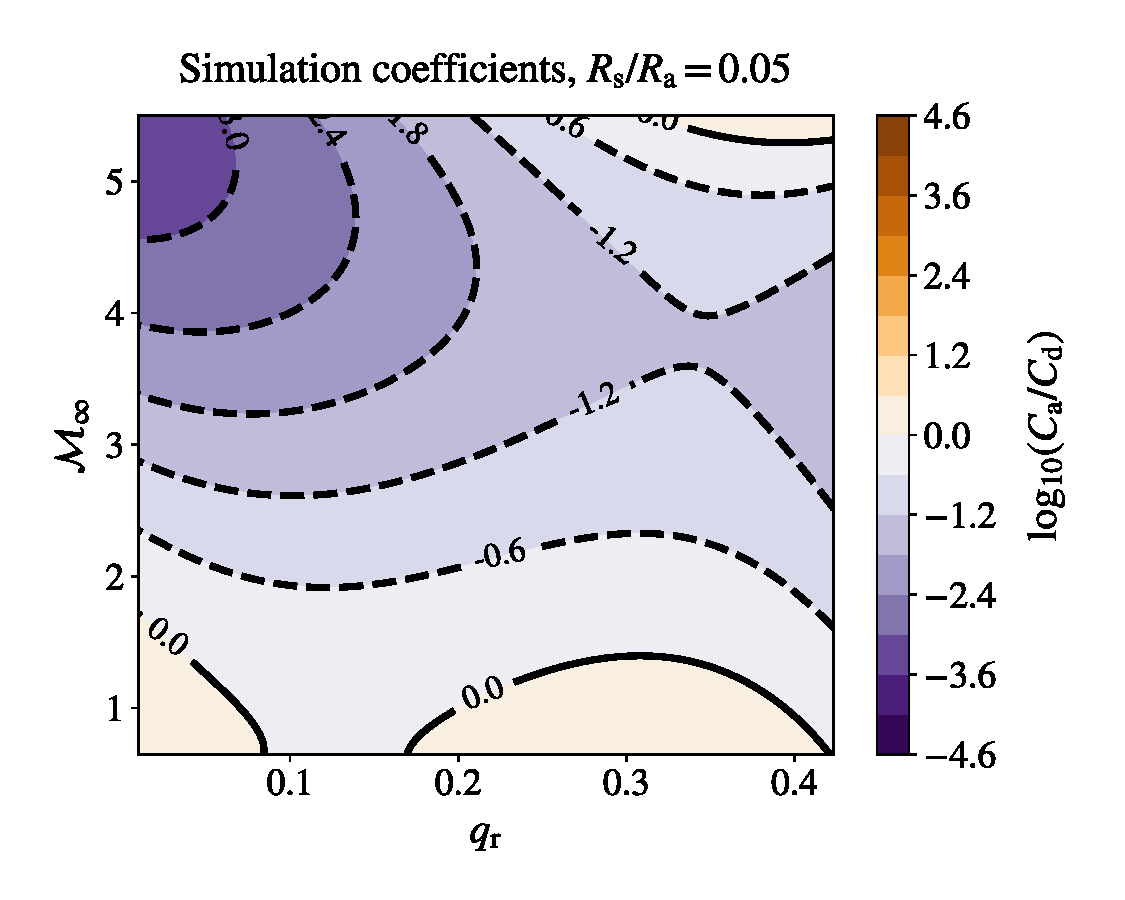
\includegraphics[width=11.5cm]{figures/common_envelope/log_ratio_mdot_drag_inc_mdotdrag_3_fit_to_runs_g43_contour_rs5e-2.pdf}
  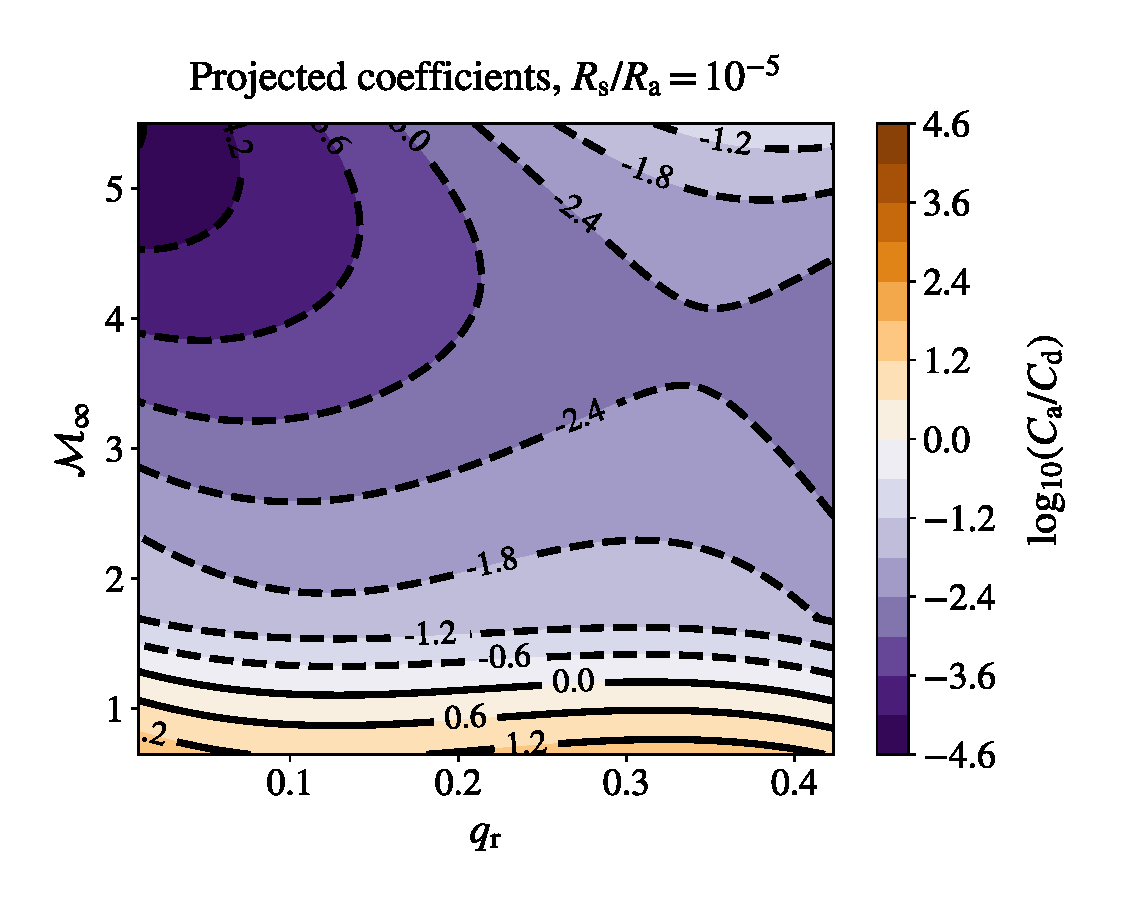
\includegraphics[width=11.5cm]{figures/common_envelope/log_ratio_mdot_drag_inc_mdotdrag_3_fit_to_runs_g43_contour_rs1e-5.pdf}
\caption{Two-dimensional contour plot of $\log_{10}(C_{\mathrm a}/C_{\mathrm d})$ in the $q_{\rm r}-\mathcal{M}_\infty$ space using numerical results from the $\gamma = 4/3$ simulations presented in this paper. The top panel shows the $(q_{\rm r}, \mathcal{M}_\infty) \rightarrow (C_{\mathrm a}, C_{\mathrm d})$ mapping for the sink size used in the simulations $R_{\rm s}/R_{\rm a} = 0.05$. The bottom panel shows the $(q_{\rm r}, \mathcal{M}_\infty) \rightarrow (C_{\mathrm a}, C_{\mathrm d})$ mapping with the coefficients extrapolated to a sink size $R_{\rm s}/R_{\rm a} = 10^{-5}$, which is more realistic for a black hole embedded in a common envelope.\label{fig:mdot_fdf_ratio_rs05_rs1e-5}}
\vspace{5mm}
\end{figure}

We observe that for the majority of the $q_{\rm r}-{\cal M}_\infty$ parameter space, $C_{\rm a}/C_{\rm d} \ll 1$, even in the direct simulation coefficients, though $C_{\rm a}/C_{\rm d}$ approaches unity as ${\cal M}_\infty\rightarrow1$. For specificity, if we use our direct (unscaled) simulation coefficients, and take the example case of a black hole involved in a $\overline{q_{\rm r}}\sim 0.1$ encounter, $C_{\rm a}/C_{\rm d} \lesssim 0.1$ for ${\cal M}_\infty \gtrsim 2$.  This is the bulk of the relevant parameter space for a dynamical inspiral if the relative velocity between the black hole and the envelope gas is similar to the Keplerian velocity (see Figure 3 and 4 of Ref. \cite{MacLeod_2015} and Figure 1 of Ref. \cite{MacLeod:2017}). If $C_{\rm a}/C_{\rm d}=0.1$, then $d\ln M_2 / d\ln E \approx 0.045$ (equation \eqref{eq:dlnMdE}), i.e., a 5\% change in the mass of the black hole due to accretion per orbital e-folding during the common envelope encounter. If this accreted mass is coherently maximally rotating, the black hole would spin up to $\chi\sim 0.15$ (if it begins with $\chi=0$). Thus, if the orbital energy changes by a factor of 25, the black hole would accrete about 15\% of its original mass (equation \eqref{eq:MEsolution}) and spin up to $\chi\sim 0.4$ (equation \eqref{eq:aspin}).

However, we have argued in Section \ref{sec:sink} that the simulated $C_{\rm a}/C_{\rm d}$ can be misleadingly high (or, alternatively is best interpreted as a strict upper limit) because the compact object radius is orders of magnitude smaller than $R_{\rm s}$. With the rescaled results of the second panel of Figure \ref{fig:mdot_fdf_ratio_rs05_rs1e-5} for $R_{\rm s} = 10^{-5} R_{\rm a}$, we see that for the same $\overline{q_{\rm r}}=0.1$ encounter in which ${\cal M}_\infty \gtrsim 2$, the ratio of the accretion to drag coefficient is $C_{\rm a}/C_{\rm d} \lesssim 10^{-2}$. This in turn implies that a black hole undergoing such a common envelope encounter accretes according to $d\ln M_2 / d\ln E \approx 0.0045$. Again, taking the example of orbital energy changing by a factor of 25, the black hole would accrete 1.4\% of its own mass and spin up to $\chi \sim 0.05$.  Even if the binary hardens by three orders of magnitude during the common-envelope phase, a non-spinning black hole would only accrete $\sim 3\%$ of its original mass and spin up to $\chi \sim 0.1$.

A possible exception to these predictions of low accreted mass and spin are black holes embedded in ${\cal M}_\infty \sim 1$ flows (involving dense stellar envelope material) and proportionately shallow density gradients. In these cases black holes can accrete at similar to the HL rate, largely because the environment is nearly homogeneous on the scale of $R_{\rm a}$. This regime of Mach numbers may be relevant to the self-regulated common-envelope inspiral phase that follows the dynamical inspiral. However, in this case, Mach numbers are lower in part because the embedded objects interact with  much lower density, higher entropy gas as the orbit starts to stabilize~(e.g., \cite{Ohlmann:2016b,Ivanova:2016, Iaconi:2018,Chamandy:2019psk}). This is presented quantitatively in Ref. \cite{Chamandy:2019psk}'s study of forces during a common envelope simulation, which showed that forces significantly decrease below those expected from the original stellar profile as the orbit stabilizes. 

The current catalog of gravitational-wave events observed by the LIGO-Virgo detectors demonstrates the existence of moderately massive black holes in binary systems~\cite{Abbott:2016blz,TheLIGOScientific:2016pea,Nitz:2018imz,Nitz:2019hdf,Biwer:2018osg,Abbott:2017vtc,Abbott:2017gyy,Abbott:2017oio,Zackay:2019tzo,Venumadhav:2019lyq,LIGOScientific:2018mvr,De:2018zrk}. Common-envelope evolution is considered to be one of the preferred channels for the formation of these binaries~\cite{Kruckow:2016tti,Belczynski:2016obo,EldridgeStanway:2016,Stevenson:2017,Mapelli:2018}. These predictions therefore have important potential implications when considering the evolutionary history of the LIGO-Virgo network's growing population of gravitational-wave merger detections. 

If the typical black hole passing through a common envelope-phase accreted a significant fraction of its own mass, and reached dimensionless spin near unity (as implied by equations \eqref{eq:MEsolution} and \eqref{eq:aspin} if $C_{\rm a}/C_{\rm d}=1$) this would have two directly observable consequences on the demographics of merging black holes. The mass gaps believed to exist in the birth distributions of black holes masses~\cite{Bailyn:1998,Kreidberg:2012,Ozel:2010,Farr:2011,Yusof:2013,Belczynski:2014,Marchant:2016,Woosley:2017} would be efficiently eradicated if black holes doubled their masses over the typical evolutionary cycle. Secondly, the average projected spins of merging black holes onto the orbital angular momentum would be large ($\chi_{\rm eff}\sim 1$ if coherently oriented) or at least broadly-distributed (if randomly oriented), contrary to the existing interpretation of spins from LIGO--Virgo black hole observations (e.g., \cite{Farr:2017uvj,Farr:2017gtv,Tiwari:2018qch,Piran_2019}), or the predictions of spins in merging binary black holes (e.g., \cite{Bavera:2019fkg,Fuller:2019sxi,Zaldarriaga:2017qkw,Kushnir:2016zee,Schroder:2018hxk,Batta:2019clm}). 

Our prediction of percent-level mass and spin accumulation yields a very different landscape of post common-envelope black holes. Our models suggest that common envelope phases should not significantly modify the natal masses or spins of black holes. If black holes are formed with non-smooth  mass distributions (including gaps or other features) or with low spin values, our models predict that these features would persist through a common envelope phase. 

\vspace{5mm}
\section{Conclusions}\label{sec:conclusions}
In this paper we have explored the effects of varying the binary mass ratio on common envelope flow characteristics, as well as coefficients of accretion and drag, using the Common Envelope Wind Tunnel setup of Ref. \cite{MacLeod:2017}. As the binary mass ratio is varied, the ratio of the gravitational focusing scale of the flow to the binary separation changes.
We have also varied the flow upstream Mach number and gas adiabatic constant, which were investigated in Ref. \cite{MacLeod:2017} and Ref. \cite{MacLeod_2015}. We have derived fitting formulae for the efficiency of accretion and drag from our simulations, and have applied these to derive implications for the mass and spin accreted by black holes during the common envelope encounter. Some key conclusions of this work are:

\begin{enumerate}
\setlength\itemsep{1em}
\item Using a systematic survey of the dimensionless parameters that characterize gas flows past objects embedded within common envelopes, we use our simplified Common Envelope Wind Tunnel hydrodynamic model to study the role of the upstream Mach number $\mathcal{M}_\infty$, enclosed mass ratio $q_{\rm r}$, and the equation of state (as bracketed by adiabatic indices $\gamma=4/3$ and $\gamma=5/3$). For each model, we derive time-averaged coefficients of accretion, $C_{\rm a}$, and drag, $C_{\rm d}$ (Tables \ref{tab:sims_43_params} and \ref{tab:sims_53_params}).

\item Upstream Mach number $\mathcal{M}_\infty$ is a proxy for the dimensionless upstream density gradient $\epsilon_\rho$ (equation \ref{eq:mach-erho}). Higher $\mathcal{M}_\infty$ flows tend to have more asymmetric geometries due to steeper density gradients (Figures \ref{fig:sims_g43_fix_q_vary_mach} and \ref{fig:sims_g53_fix_q_vary_mach}). This transition in flow morphology is accompanied by higher drag coefficients but lower accretion coefficients (Figure \ref{fig:datapoints_Ca_Cd_vs_mach_g43_g53_sims}). 

\item The gas equation of state, parameterized here by the adiabatic index of ideal-gas hydrodynamic models $\gamma$, primarily affects the concentration of gas flow around the accretor. When $\gamma = 5/3$, pressure gradients partially act against gravitational focusing (Figure \ref{fig:sims_g53_fix_q_vary_mach} as compared to \ref{fig:sims_g43_fix_q_vary_mach}) and reduce coefficients of both accretion and drag by a factor of a few relative to $\gamma=4/3$ (Figure \ref{fig:datapoints_Ca_Cd_vs_mach_g43_g53_sims}). 

\item The binary mass ratio affects the ratio of gravitational focusing length to binary separation, $R_{\rm a}/a$, shown in equation \eqref{eq:Ra_asfunc_a} and Figure \ref{fig:ra-q}. As a result, larger mass ratio cases have weaker focusing of the flow around the embedded object, because gravitational focusing acts over a smaller number of gravitational focusing lengths to concentrate the flow (Figure \ref{fig:sims_fix_mach_vary_q}). The consequences of this distinction are reduced drag (lower $C_{\rm d}$) because of reduced momentum exchange with the flow, and, especially in the highest $\mathcal{M}_\infty$ cases, higher capture fractions (increased $C_{\rm a}$) because gas does not receive a sufficient gravitational slingshot to escape the accretor (Figure \ref{fig:datapoints_Ca_Cd_vs_mach_g43_g53_sims}).

\item The size of a typical accretor is a factor of $10^3$ to $10^8$ times smaller than the gravitational focusing radius, $R_{\rm a}$. Due to the limits of computational feasibility, our default numerical models adopt $R_{\rm s}/ R_{\rm a}=0.05$. We re-run the $\gamma=4/3$ models with $R_{\rm s}/ R_{\rm a}=0.025$ and $R_{\rm s}/ R_{\rm a}=0.0125$. We find that drag coefficients are insensitive to $R_{\rm s}$, but accretion coefficients have a dependence which we parameterize with a power-law slope, $\alpha_{\dot M}$ (Figure \ref{fig:sink}).
These scalings allow us to extend our Common Envelope Wind Tunnel results to more astrophysically realistic scenarios.

\item The amount of mass accreted by a compact object during a common envelope phase is coupled to the degree of orbital tightening, as per the HL theory \cite[and Section \ref{sec:coupled}]{Chevalier:1993,Brown:1995,Bethe:1998}. Angular momentum carried by the accreted mass may also spin up the object. Therefore, the values of $C_{\rm a}$ and $C_{\rm d}$ are crucial in determining the mass and spin accrued by embedded objects during the common envelope phase (specifically, the ratio $C_{\rm a}/C_{\rm d}$ sets the mass gain per unit orbital tightening, equation \eqref{eq:dlnMdE}). In the Hoyle Lyttton scenario, where $C_{\rm a}/C_{\rm d}=1$, the typical black hole immersed in a common envelope would gain on the order of its own mass and spin up to $\chi=1$.

\item Our simulation results that $C_{\rm a}/C_{\rm d} \ll 1$ suggest that black holes spiralling in through common envelopes accumulate less than 1\% mass per logarithmic change in orbital energy. In a typical event, this might correspond to a 1--2\% growth in black-hole mass and spin-up to a dimensionless spin of $\approx$ 0.05 for an initially non-spinning black hole (Figure \ref{fig:mdot_fdf_ratio_rs05_rs1e-5} and Section \ref{sec:LIGO}). Thus, our predictions suggest that common-envelope phases should not modify the mass and spin distributions of black holes from their natal properties.
\vspace{0.5cm}
\end{enumerate}

The hydrodynamic models presented in this paper have numerous simplifications relative to the complex, time-dependent geometry and flow likely realized in a common envelope interaction. Nonetheless, they allow us to discover trends by systematically exploring the parameter space that may arise in typical interactions. A companion paper, Ref. \cite{Rosa:2020}, considers the stellar evolutionary conditions for donor stars in common envelope systems under which this dimensionless treatment is useful. 

The ratio of accretion to drag coefficients (relative to their HL values) determines the amount of mass accretion during the dynamical inspiral phase of common envelope evolution. If our finding that $C_{\rm a}/C_{\rm d} \ll 1$ is correct, then the implications of this for gravitational wave observables are significant. In particular, if the birth mass distributions of black holes have non-smooth features, including gaps, or if black holes have low natal spins, these characteristic distributions will be preserved after the common envelope phase.


\clearpage
\section{Appendix}
\subsection{Fitting Formulae To Coefficients of Drag and Accretion}\label{subsec:fits}
We present fitting formulae for the coefficients of accretion $C_{\mathrm a}$ and drag force $C_{\mathrm d}$ as a function of the mass ratio $q_{\rm r}$ and upstream Mach number $\mathcal{M}_\infty$ from both our $\gamma = 4/3$ and $\gamma = 5/3$ simulations. Fits are constructed using the $q_{\rm r}$, $\mathcal{M}_\infty$, $C_{\mathrm a}$, $C_{\mathrm d}$ datasets presented in Tables \ref{tab:sims_43_params} and \ref{tab:sims_53_params} in Sec.~\ref{sec:hydro_sims}. The fits show a mapping from the simulation results to the input parameters for the parameter space we have explored. For the $\gamma = 4/3$ simulations, we use third order polynomials as fitting functions for both log$_{10}C_{\mathrm a}$ and log$_{10}C_{\mathrm d}$, that are  expressed as follows

\begin{equation}
%\begin{adjustwidth}{-0.5mm}{}
\label{eq:logmdot_g43}
\begin{split}
\log_{10} C_{\mathrm a} = a_1 + a_2 q_{\rm r} + a_3\mathcal{M}_\infty + a_4 q_{\rm r}\mathcal{M}_\infty
+ a_5 q_{\rm r}^2 + a_6 \mathcal{M}_\infty^2 
+ a_7 q_{\rm r} \mathcal{M}_\infty^2 + a_8 q_{\rm r}^2\mathcal{M}_\infty \\ + a_9 q_{\rm r}^3 + a_{10} \mathcal{M}_\infty^3
\end{split}
%\end{adjustwidth}
\end{equation}

\begin{equation}
\label{eq:logdrag_g43}
\begin{split}
\log_{10} C_{\mathrm d} = d_1 + d_2 q_{\rm r} + d_3 \mathcal{M}_\infty + d_4 q_{\rm r}\mathcal{M}_\infty + d_5 q_{\rm r}^2 + d_6 \mathcal{M}_\infty^2
+ d_7 q_{\rm r}\mathcal{M}_\infty^2 + d_8 q_{\rm r}^2\mathcal{M}_\infty \\ + d_9 q_{\rm r}^3 + d_{10} \mathcal{M}_\infty^3
\end{split}
\end{equation}
                

Accumulation of material from accretion onto an embedded compact object requires either that the object be a black hole, or the presence of an effective cooling channel if the object has a surface. In the case of objects with a surface, accretion releases gravitational potential energy and generates feedback. Our simulations include a completely absorbing central boundary condition, and therefore our setup is appropriate for calculating accretion rates for cases where the feedback from accretion can be neglected. The fitting formulae from the $\gamma = 4/3$ simulations presented above are applicable for systems where a black hole is inspiraling inside the envelope of a more massive giant branch star. This is because, taking into account the minimum mass of black holes and the fact that the envelope must belong to a more massive giant star than the embedded object, the mass of the giant star in this scenario would be greater than $\sim 10 M_\odot$. As mentioned earlier, the flow of material in such high mass stars would be represented by a $\gamma = 4/3$ equation of state.  

\begin{figure*}
  \centering
  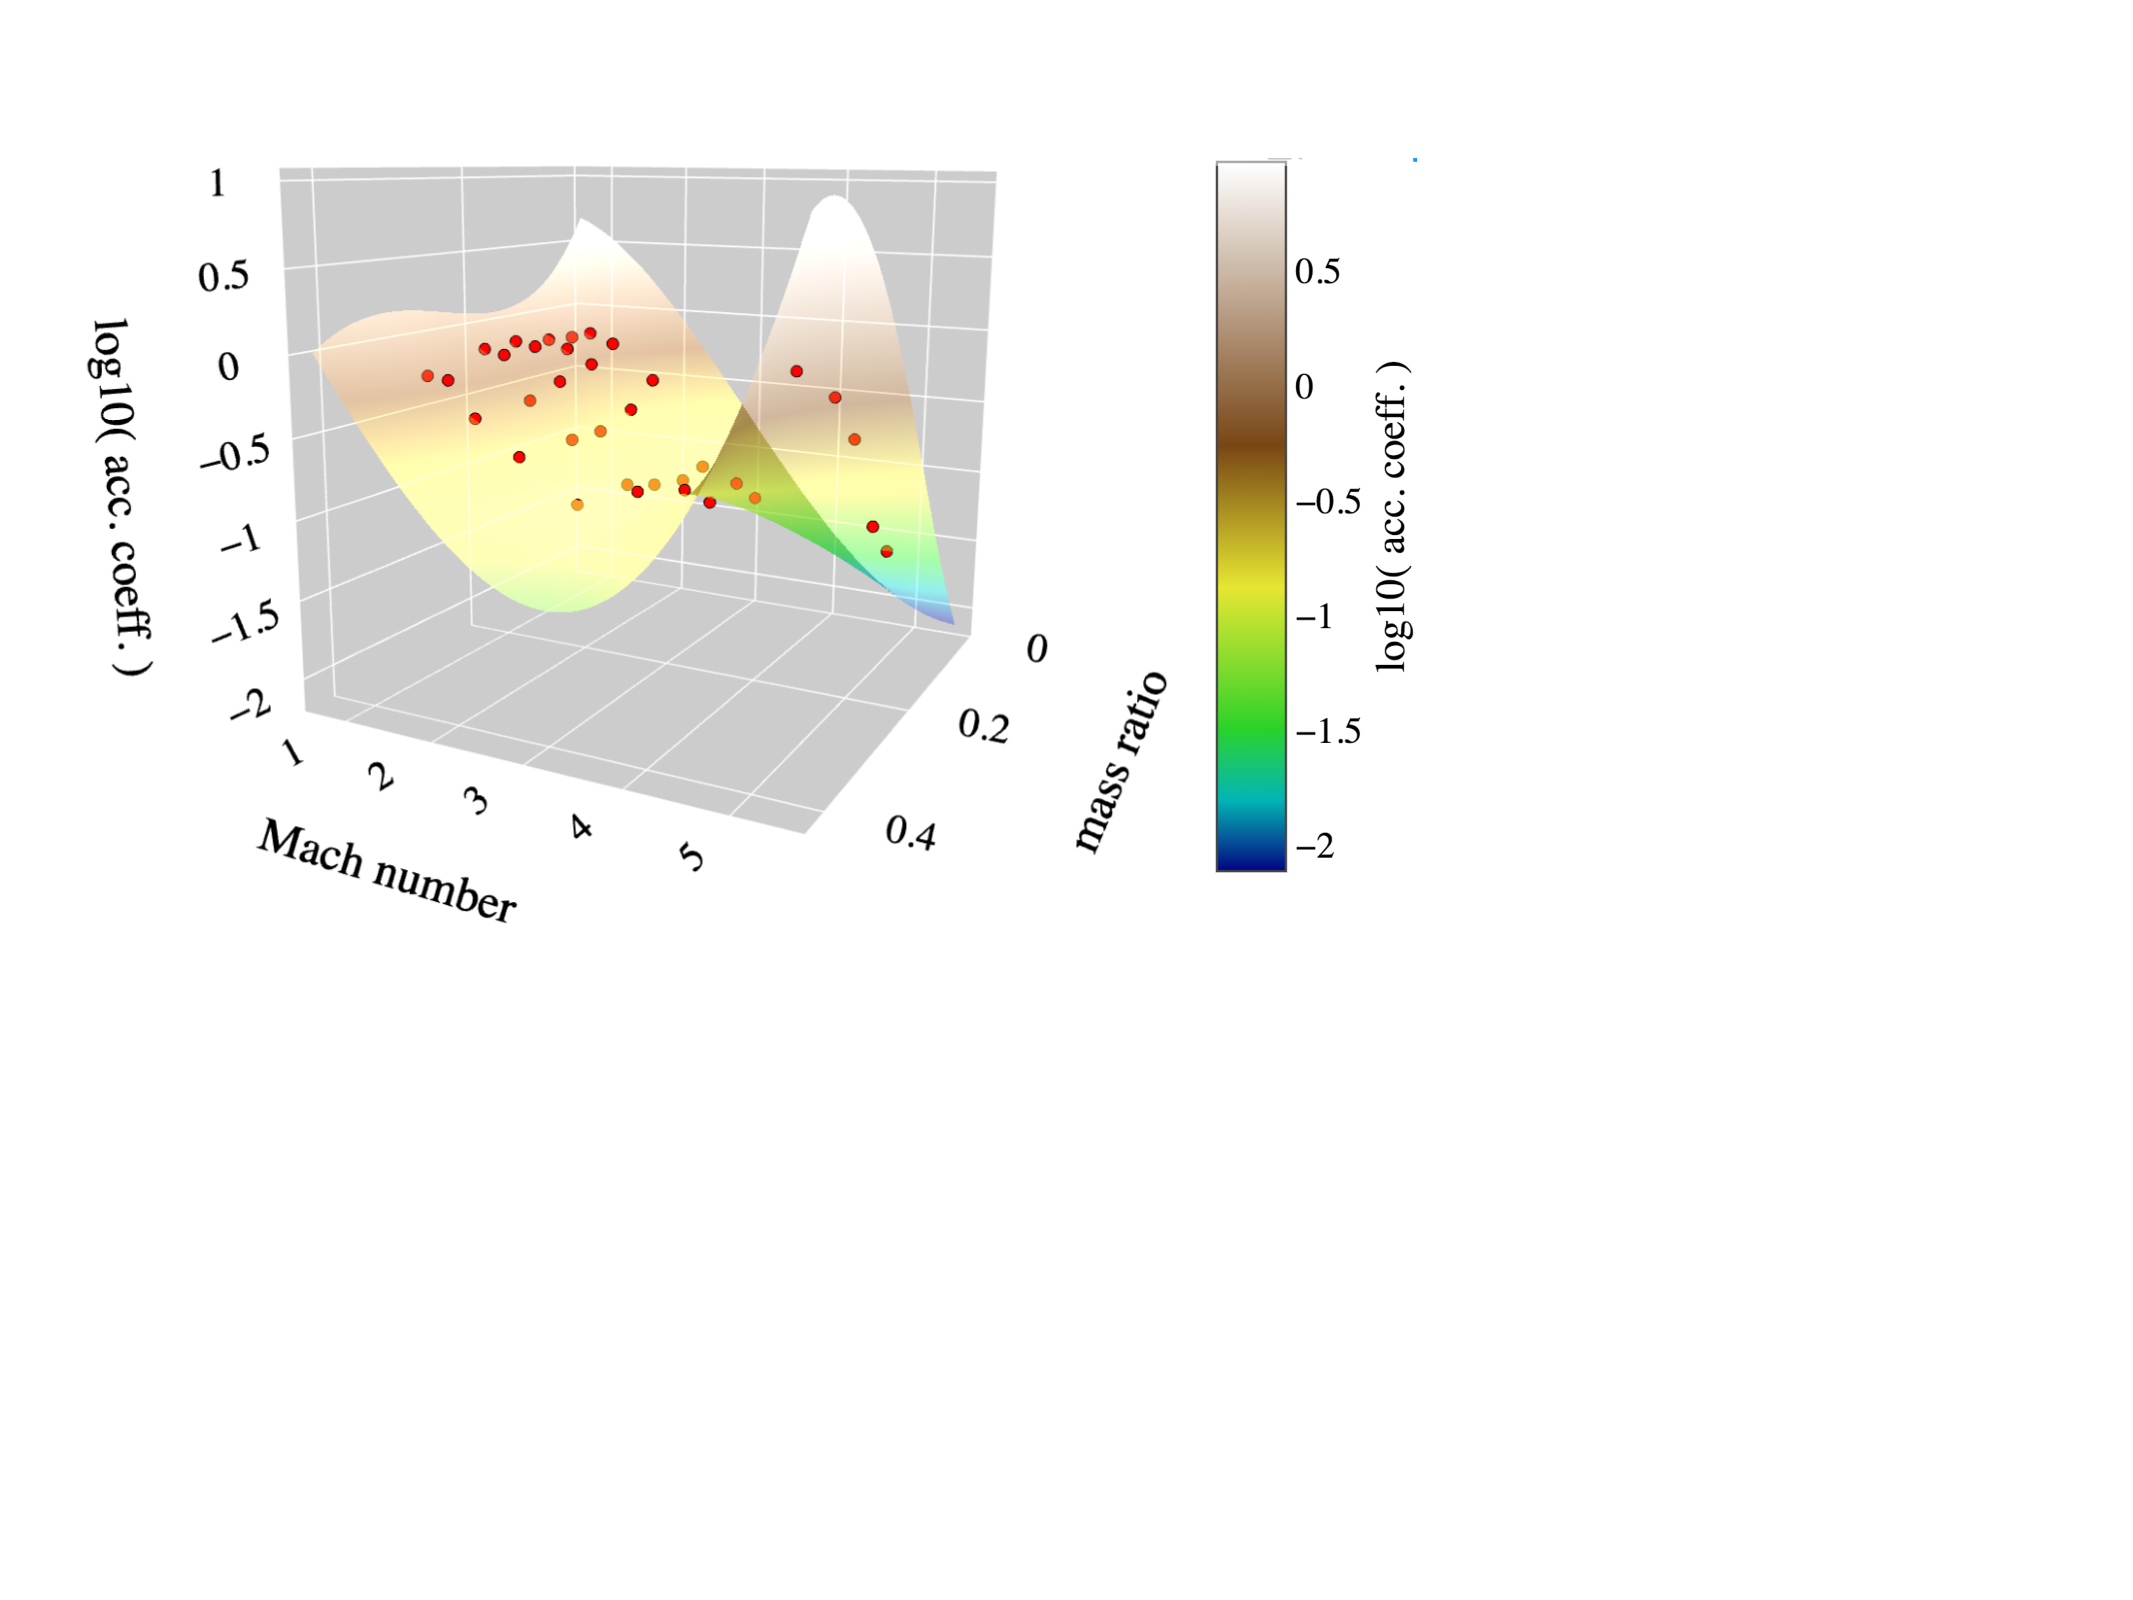
\includegraphics[width=14cm]{figures/common_envelope/logmdot_order3_g43.pdf}
\caption{Relation between the coefficient of accretion, mass ratio, and upstream Mach number---$\log_{10}C_{\mathrm a} (q_{\rm r}, \mathcal{M}_\infty)$ for $(\Gamma, \gamma) = (4/3, 4/3)$ flows. The red dots represent the $\log_{10}C_{\mathrm a}$ results obtained from the hydrodynamic simulations with $q_{\rm r}$ and $\mathcal{M}_\infty$ parameters. The three-dimensional surface shows the best fitting third-order polynomial relation of $\log_{10}C_{\mathrm a}$ in terms of $(q_{\rm r}, \mathcal{M}_\infty)$.\label{fig:logmdot_g43}}
\end{figure*}

\begin{figure*}
  \centering
  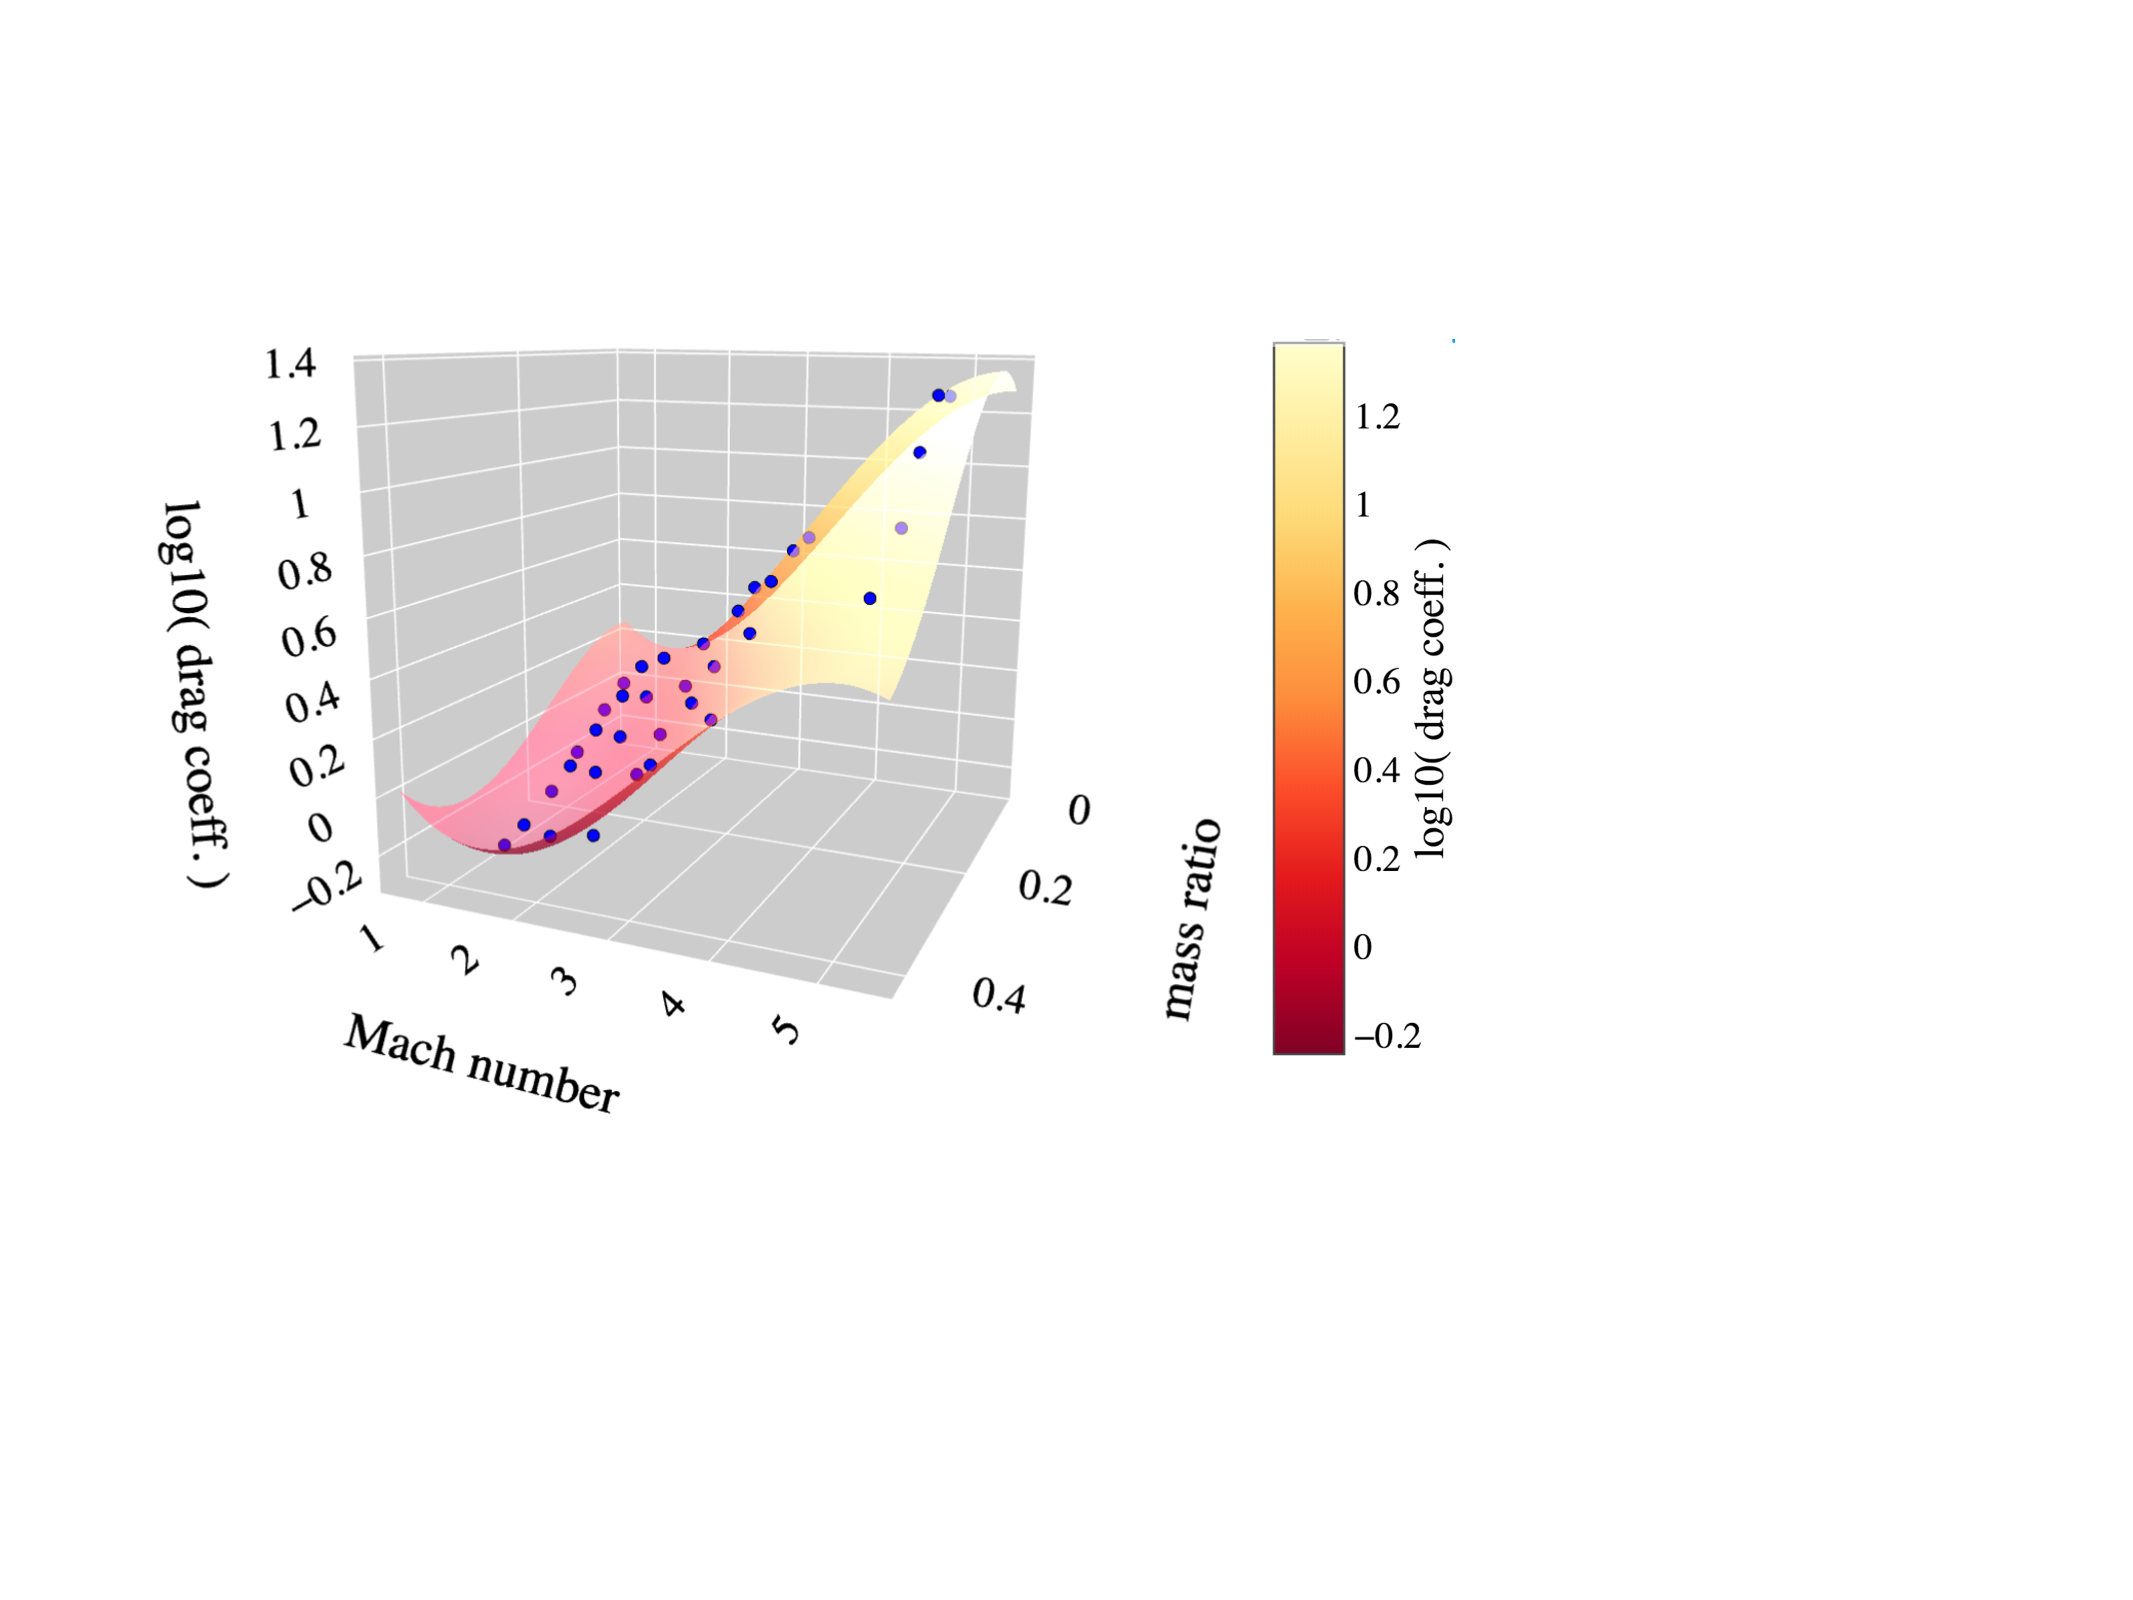
\includegraphics[width=14cm]{figures/common_envelope/logdrag_order3_g43_inc_mdotdrag.pdf}
\caption{Relation between the coefficient of drag, mass ratio, and upstream Mach number---$\log_{10}C_{\mathrm d} (q_{\rm r}, \mathcal{M}_\infty)$ for $(\Gamma, \gamma) = (4/3, 4/3)$ flows. The blue dots represent the $\log_{10}C_{\mathrm d}$ results obtained from the hydrodynamic simulations with $q_{\rm r}$ and $\mathcal{M}_\infty$ parameters. The three-dimensional surface shows the best fitting third-order polynomial relation of $\log_{10}C_{\mathrm d}$ in terms of $(q_{\rm r}, \mathcal{M}_\infty)$.\label{fig:logdrag_g43}}
\end{figure*}

For the $\gamma=5/3$ simulations, we use second order polynomials as fitting functions for both log$_{10}C_{\mathrm a}$  and log$_{10}C_{\mathrm d}$, which can be expressed as

\begin{equation}
\label{eq:logmdot_g53}
\begin{split}
\log_{10} C_{\mathrm a} = a_1 + a_2 q_{\rm r} + a_3 \mathcal{M}_\infty + a_4 q_{\rm r}\mathcal{M}_\infty + a_5 q_{\rm r}^2 + a_6 \mathcal{M}_\infty^2
\end{split}
\end{equation}

\begin{equation}
\label{eq:logdrag_g53}
\begin{split}
\log_{10} C_{\mathrm d} = d_1 + d_2 q_{\rm r} + d_3 \mathcal{M}_\infty + d_4 q_{\rm r}\mathcal{M}_\infty + d_5 q_{\rm r}^2 + d_6 \mathcal{M}_\infty^2
\end{split}
\end{equation}


These fitting formulae from the $\gamma = 5/3$ simulations are applicable for systems where a white dwarf or a main sequence star is inspiraling inside the envelope of a more massive giant branch star. The giant star in this case would be less massive than that in the $\gamma = 4/3$ systems. However, despite flow convergence in such systems, we do not expect significant mass accumulation from accretion onto the compact object due to the lack of an apparent cooling mechanism. Main sequence stars and white dwarfs are not compact enough to promote cooling channels such as neutrino emission, mediating the luminosity of the accretion onto the neutron stars. Also, the common envelope flows are optically thick, preventing the escape of heat through photon diffusion. It would be more appropriate to model these objects with a hard-surface boundary condition than an absorbing boundary condition.

The least square solutions we obtain for the fits to the $\gamma = 4/3$ and $\gamma = 5/3$ datasets are tabulated in Table \ref{tab:sims_43_fits} and Table \ref{tab:sims_53_fits} respectively. In Figures ~\ref{fig:logmdot_g43}, \ref{fig:logdrag_g43}, ~\ref{fig:logmdot_g53}, and ~\ref{fig:logdrag_g53} we present the $\log_{10}C_{\mathrm a} (q_{\rm r}, \mathcal{M}_\infty)$ and $\log_{10}C_{\mathrm d} (q_{\rm r}, \mathcal{M}_\infty)$ datasets from the $\gamma = 4/3$ and $\gamma = 5/3$ simulations. Overlaid are the best fit surfaces as presented in Eqns.~\ref{eq:logmdot_g43}, \ref{eq:logdrag_g43}, \ref{eq:logmdot_g53} and \ref{eq:logdrag_g53} above. Interactive versions of these figures can be viewed at \url{https://soumide1102.github.io/common-envelope-hydro-paper}.

\begin{table}[h]
\centering
\begin{adjustwidth}{-1.5cm}{}
\begin{tabular}{lccccccccc} 
\hline\hline
\rule{0pt}{3ex}
$a_1$ & $a_2$ & $a_3$ & $a_4$ & $a_5$ & $a_6$ & $a_7$ & $a_8$ & $a_9$ & $a_{10}$ \\
\hline
\rule{0pt}{3ex}%
\vspace*{0.1cm}
0.8169 & -9.9784 & 0.1382 & -0.4803 & 46.9755 & -0.3330 & 0.6713 & -4.1620 & -58.9379 & 0.0379 \\
\hline\hline
\rule{0pt}{3ex}
$d_1$ & $d_2$ & $d_3$ & $d_4$ & $d_5$ & $d_6$ & $d_7$ & $d_8$ & $d_9$ & $d_{10}$ \\
\hline
\rule{0pt}{3ex}%
\vspace*{0.1cm}
0.5510 & 0.4502 & -0.6741 & 0.5946 & -14.9500 & 0.3159 & -0.0203 & -1.7043 & 30.4494 & -0.0309 \\
\hline
\end{tabular}
\caption{Coefficients of fitting formula for the efficiency of accretion and drag from $\gamma = 4/3$ simulations: least square solutions for the $\log_{10} C_{\mathrm a}$ and $\log_{10} C_{\mathrm d}$ third-order polynomial fits.}
\label{tab:sims_43_fits}
\end{adjustwidth}
\end{table}

\begin{table}[h]
\centering\begin{tabular}{lccccc}
\hline\hline
\rule{0pt}{3ex}
$a_1$ & $a_2$ & $a_3$ & $a_4$ & $a_5$ & $a_6$ \\
\hline
\rule{0pt}{3ex}%
\vspace*{0.1cm}
0.9184 & -0.9619 & -1.2057 & 1.2247 & -2.480 & 0.1150233 \\
\hline\hline
\rule{0pt}{3ex}
$d_1$ & $d_2$ & $d_3$ & $d_4$ & $d_5$ & $d_6$ \\
\hline
\rule{0pt}{3ex}%
\vspace*{0.1cm}
-0.1552 & -3.0323 & 0.2756 & 0.1976 & 1.4186 & -0.0092 \\
\hline
\end{tabular}
\caption{Coefficients of fitting formula for the efficiency of accretion and drag from $\gamma = 5/3$ simulations: least square solutions for the $\log_{10} C_{\mathrm a}$ and $\log_{10} C_{\mathrm d}$ second-order polynomial fits.}
\label{tab:sims_53_fits}
\end{table}

\begin{figure*}
  \centering
  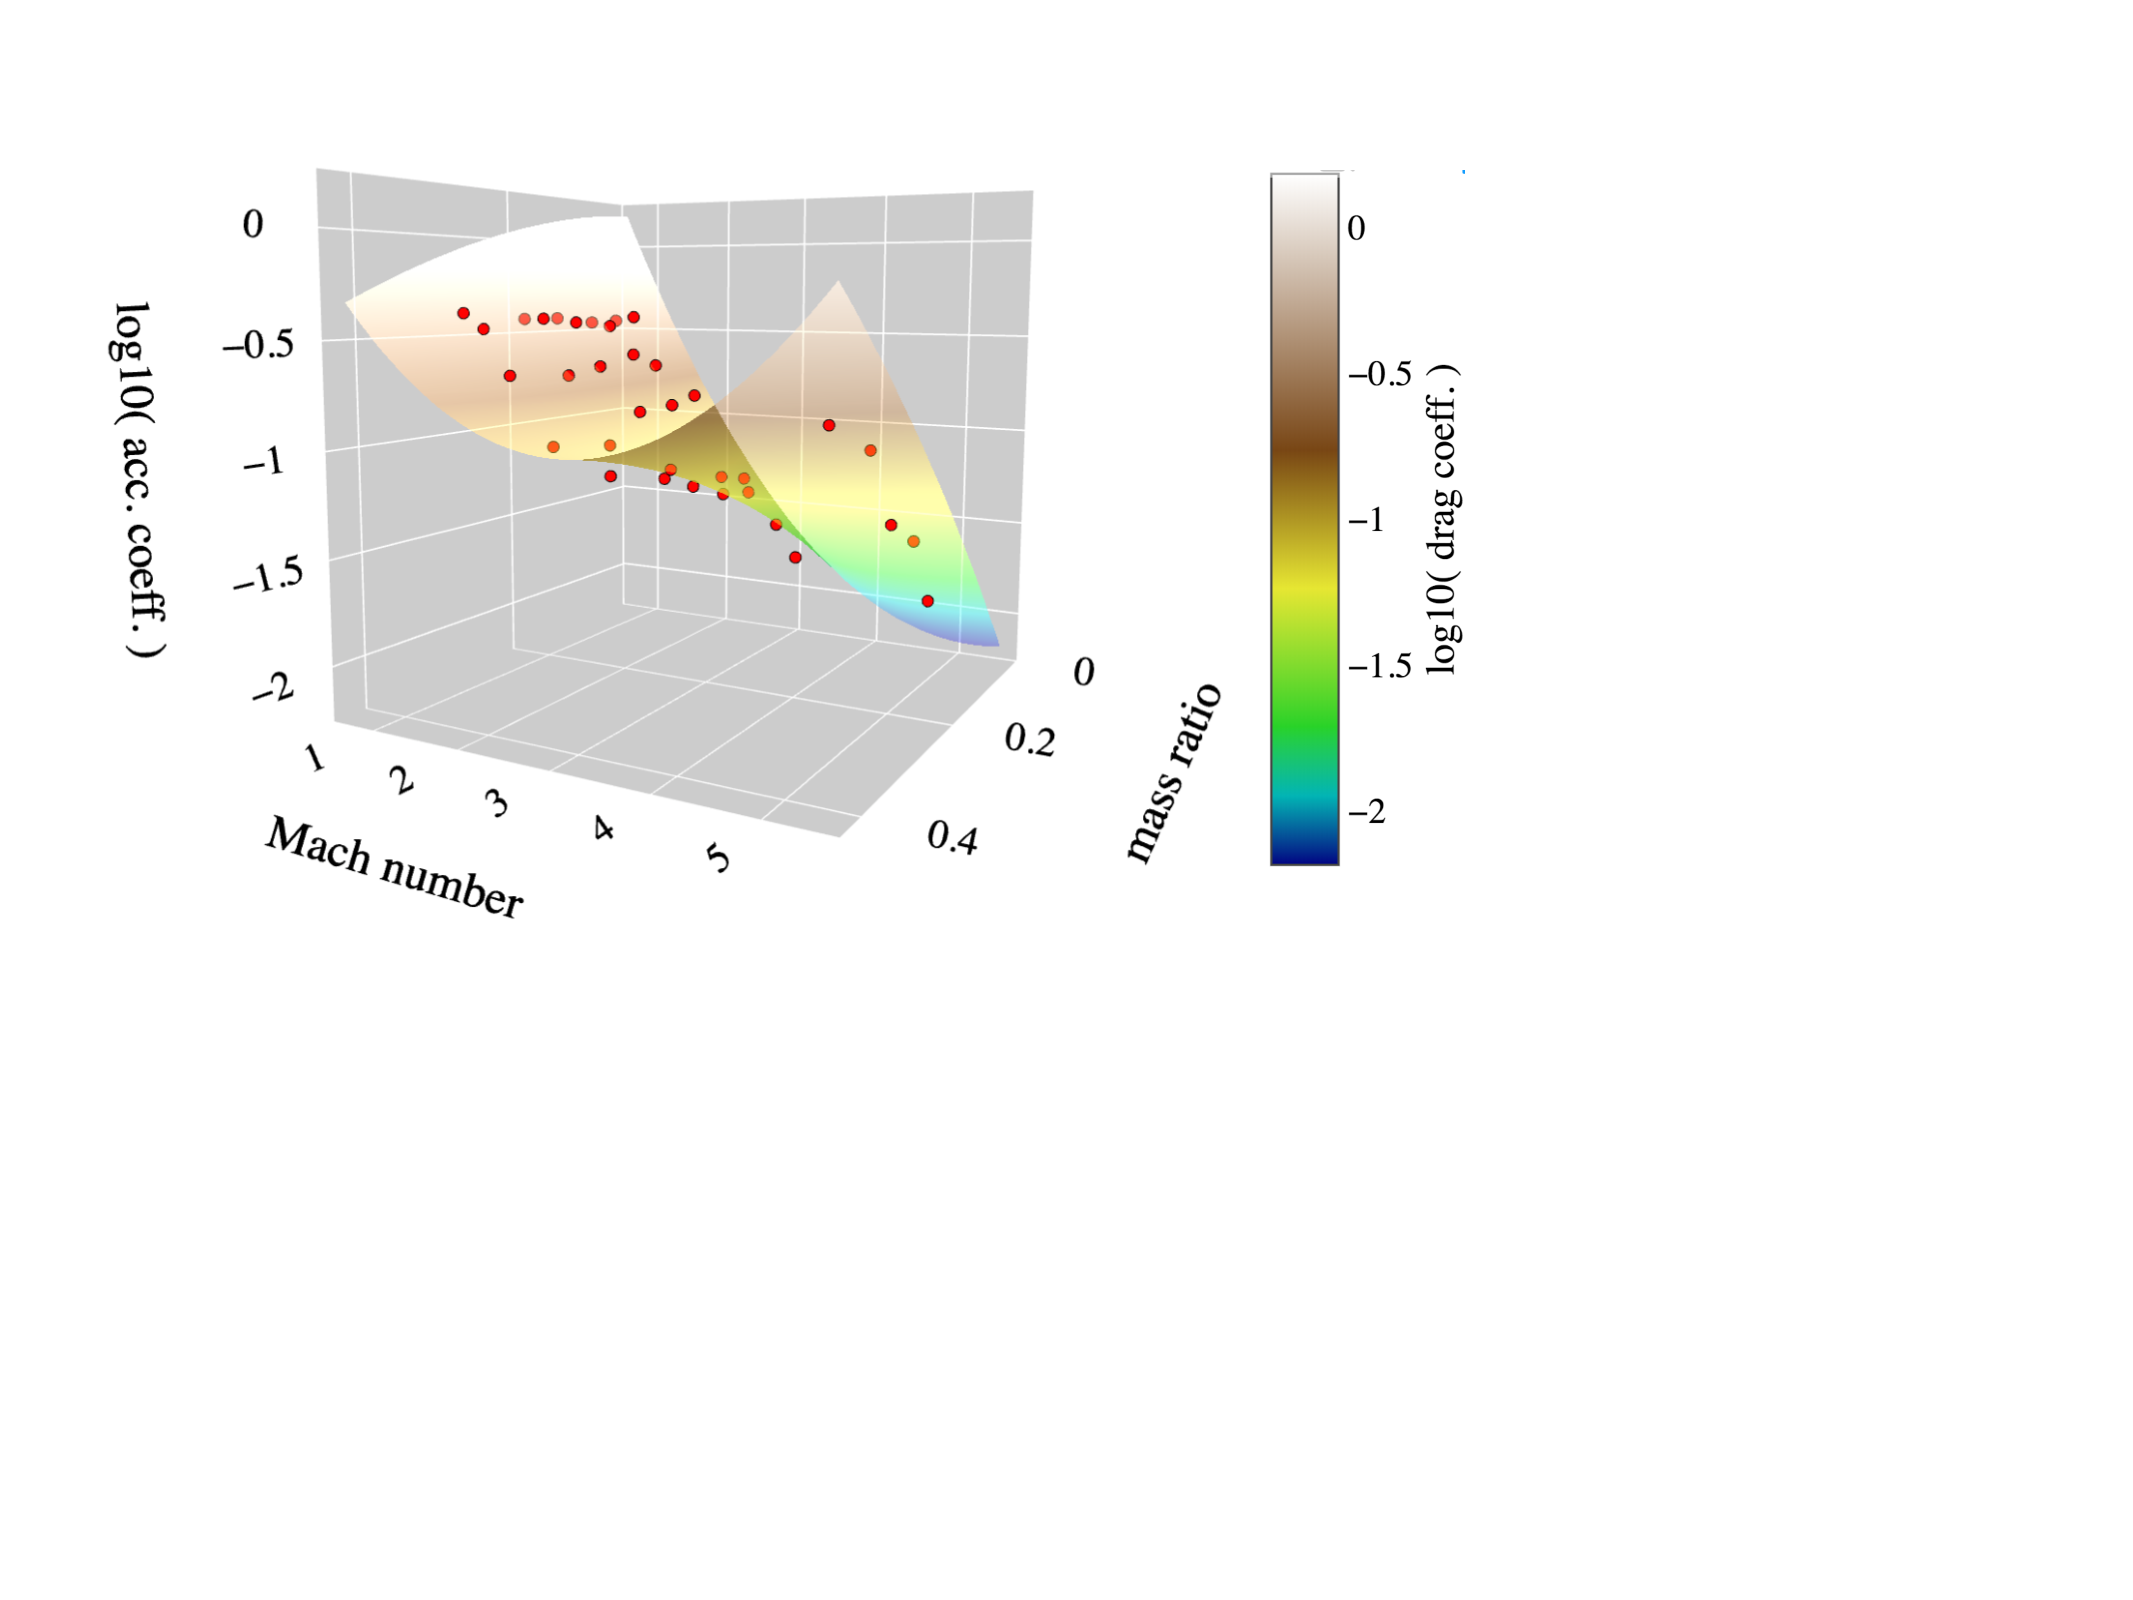
\includegraphics[width=14cm]{figures/common_envelope/logmdot_order2_g53.pdf}
\caption{Relation between the coefficient of accretion, mass ratio, and upstream Mach number---$\log_{10}C_{\mathrm a} (q_{\rm r}, \mathcal{M})$ for $(\Gamma, \gamma) = (5/3, 5/3)$ flows. The red dots represent the $\log_{10}C_{\mathrm a}$ results obtained from the hydrodynamic simulations with $q_{\rm r}$ and $\mathcal{M}_\infty$ parameters. The three-dimensional surface shows the best fitting second-order polynomial relation of $\log_{10}C_{\mathrm a}$ in terms of $(q_{\rm r}, \mathcal{M}_\infty)$.\label{fig:logmdot_g53}}.
\end{figure*}

\begin{figure*}
 \centering
 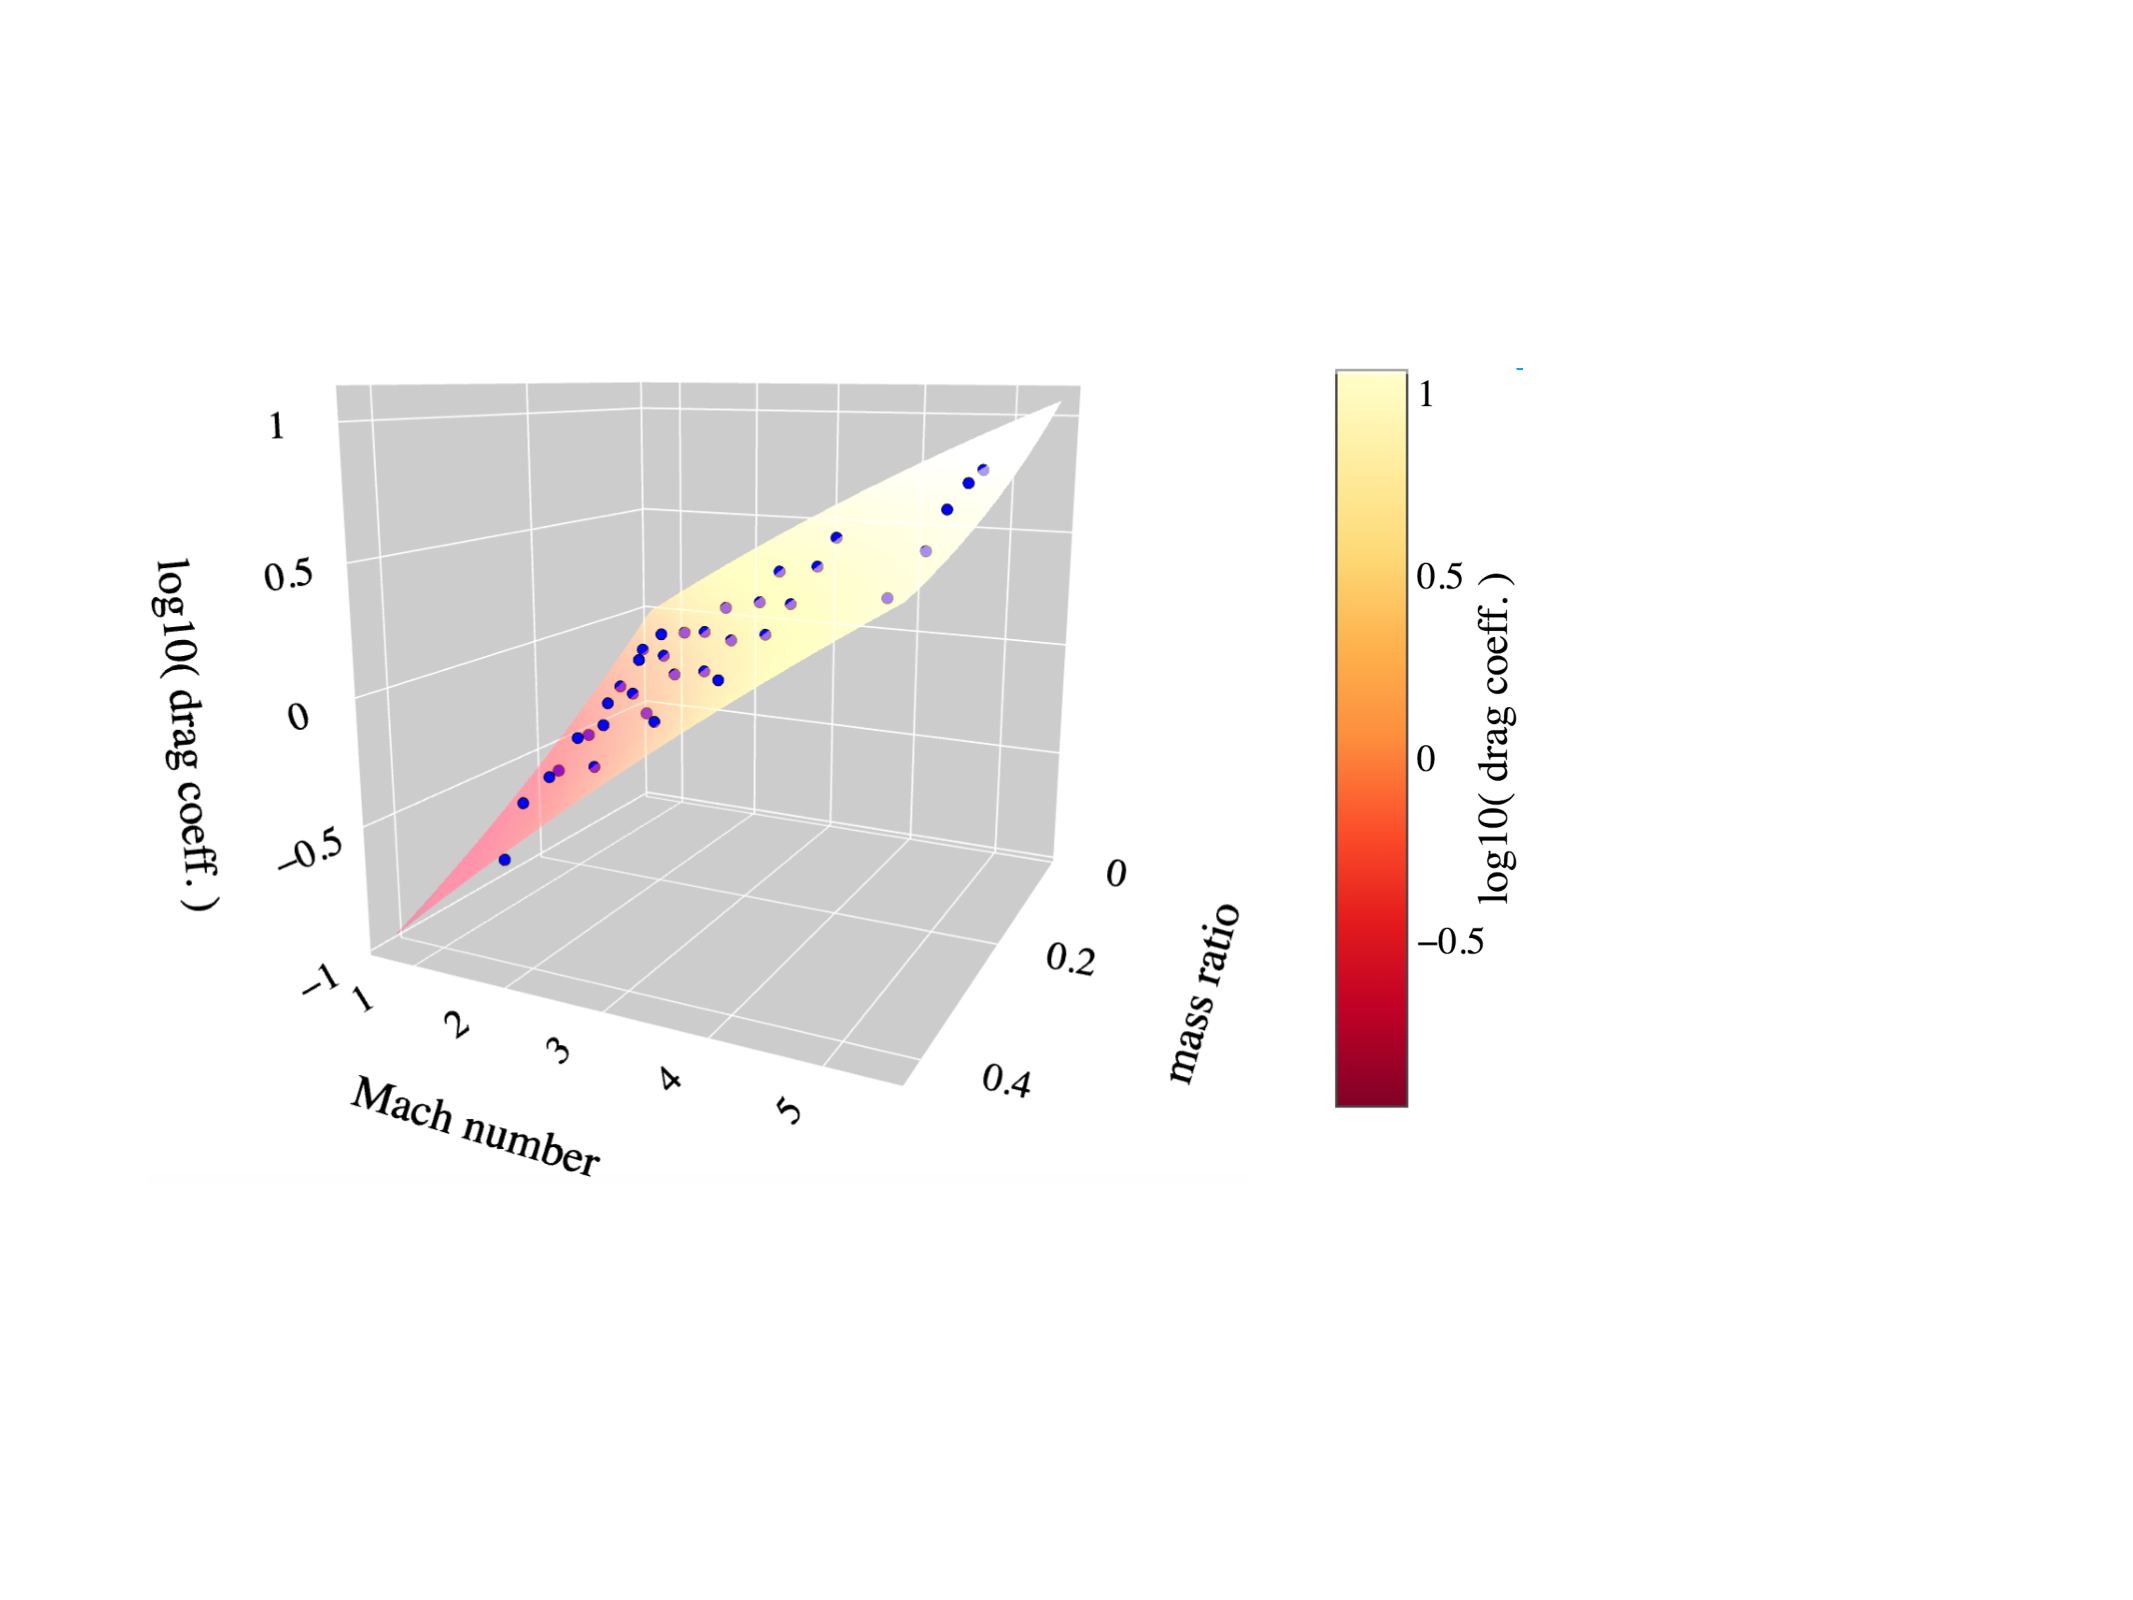
\includegraphics[width=14cm]{figures/common_envelope/logdrag_order2_g53_inc_mdotdrag.pdf}\caption{Relation between the coefficient of drag, mass ratio, and upstream Mach number---$\log_{10}C_{\mathrm d} (q_{\rm r}, \mathcal{M}_\infty)$ for $(\Gamma, \gamma) = (5/3, 5/3)$ flows. The blue dots represent the $\log_{10}C_{\mathrm d}$ results obtained from the hydrodynamic simulations with $q_{\rm r}$ and $\mathcal{M}_\infty$ parameters. The three-dimensional surface shows the best fitting second-order polynomial relation of $\log_{10}C_{\mathrm d}$ in terms of $(q_{\rm r}, \mathcal{M}_\infty)$.\label{fig:logdrag_g53}}.
\end{figure*}

\subsection{Comparison with other studies measuring drag forces\label{sec:compare_drag}}
Several studies have looked at the evolution of drag forces in common envelope interactions with numerical simulations and analytical modeling, and have compared them to the linear estimates from the Hoyle-Lyttleton formalism. In our simulations, we have modeled the regime where the upstream Mach numbers are greater than one. This limits the applicability of our results to the dynamical inspiral phase, during which the embedded object falls supersonically through the common envelope. The resulting gaseous dynamic friction forces have been modeled analytically in Ref. \cite{1999ApJ...513..252O} and numerically, in the context of common envelope phases, in Ref. \cite{Staff:2016}, Ref. \cite{Reichardt:2019}, and Ref. \cite{Chamandy:2019psk}, allowing comparison of their results with those from our work.

Ref. \cite{1999ApJ...513..252O} used time-dependent linear perturbation theory to evaluate the dynamical friction force on a massive perturber in an infinite, homogeneous, gaseous medium, both when moving  supersonically and subsonically. Ref. \cite{1999ApJ...513..252O}'s results define the strength of the dynamical friction relative to the size of the wake the object has created.

Among the global simulations of common envelope phases, Ref. \cite{Staff:2016} modeled an extreme mass ratio system ($q~\approx 0.003$), with gas adiabatic index $\gamma = 5/3$. In the supersonic regime, their numerical drag force is $\approx~2-3$ times larger than the HL drag force, as described by Eq. ~\ref{eq:fHL}. Ref. \cite{Reichardt:2019} modeled a moderate mass ratio regime, $q~\approx 0.6$. The numerical drag forces obtained from their simulation were within a factor of $\approx 2$ of the drag forces calculated using the analytical approximation from the HL formalism (Eq.~\ref{eq:fHL}), which is in agreement with Ref. \cite{Staff:2016}. Ref. \cite{Chamandy:2019psk} performed global simulations for three different mass ratio cases, $q = 1/2, 1/4, 1/8$, with a gas adiabatic constant $\gamma = 5/3$. At their smallest $q$ value of $1/8$, they find that the Bondi-Hoyle-Lyttleton estimates provide a good approximation for the drag force in their simulation. The differences between the simulation results and the Bondi-Hoyle-Lyttleton estimates increase with increasing $q$ values, with a factor 10 difference at their largest $q$ value of $1/2$. 

In Figure \ref{fig:drag_compare}, we show the evolution of the drag forces (normalized by $[4\pi \rho_\infty (GM_2)^2/c_{\rm s, \infty}^2]$) as a function of Mach numbers. We compare results obtained using the analytical approach in Ref. \cite{1999ApJ...513..252O} with results obtained using the numerical approaches in Ref. \cite{Staff:2016}, Ref. \cite{Chamandy:2019psk}, and this work. For the ``Ostriker '99'' curve, we use Equations 14 and 15 of Ref. \cite{1999ApJ...513..252O}, with $\ln{(c_{\rm s}t/r_{\rm min})} = 4$, to obtain $F_{\rm drag}/[4\pi \rho_\infty (GM_2)^2/v_{\infty}^2] (\mathcal{M}_\infty)$, then divide $F_{\rm drag}/[4\pi \rho_\infty (GM_2)^2/v_{\infty}^2] (\mathcal{M}_\infty)$ by $\mathcal{M}_\infty^2$ to obtain $F_{\rm drag}/[4\pi \rho_\infty (GM_2)^2/c_{\rm s, \infty}^2] (\mathcal{M}_\infty)$. For the ``Staff+ '16'' curve, we use Figure 4 in Ref. \cite{Staff:2016} to extract the $F_{\rm drag}/[4\pi \rho_\infty (GM_2)^2/c_{\rm s, \infty}^2] - \mathcal{M}_\infty$ data. We divide the numerical drag force time series obtained from their high resolution RGB simulations by the analytical drag force (including pressure effects) time series, to extract  $F_{\rm drag}/[4\pi \rho_\infty (GM_2)^2/v_{\infty}^2] (t)$. We then divide $F_{\rm drag}/[4\pi \rho_\infty (GM_2)^2/v_{\infty}^2] (t)$ by the square of their Mach number time series data to obtain $F_{\rm drag}/[4\pi \rho_\infty (GM_2)^2/c_{\rm s, \infty}^2] (t)$, and plot $F_{\rm drag}/[4\pi \rho_\infty (GM_2)^2/c_{\rm s, \infty}^2] (\mathcal{M}_\infty)$. For the ``Chamandy+ '19'' curve, we use the $q = 1/8$ panels from Figures 4 and 5 in Ref. \cite{Chamandy:2019psk} to extract the $F_{\rm drag}/[4\pi \rho_\infty (GM_2)^2/c_{\rm s, \infty}^2] - \mathcal{M}_\infty$ data. We divide their $R_{\rm a} (t)$ by $H_\rho (t)$ data to get $\epsilon_\rho (t)$, and use Equation \ref{eq:mach-erho} to get $\mathcal{M}_\infty (t)$ from ($\epsilon_\rho (t)$, $q$). We divide their numerical drag force time series by their analytical drag force time series (based on the Bondi-Hoyle-Lyttleton theory), to obtain $F_{\rm drag}/[4\pi \rho_\infty (GM_2)^2/v_{\infty}^2] (t)$, further divide $F_{\rm drag}/[4\pi \rho_\infty (GM_2)^2/v_{\infty}^2] (t)$ by $\mathcal{M}_\infty (t)^2$ to obtain $F_{\rm drag}/[4\pi \rho_\infty (GM_2)^2/c_{\rm s, \infty}^2] (t)$, and plot $F_{\rm drag}/[4\pi \rho_\infty (GM_2)^2/c_{\rm s, \infty}^2] (\mathcal{M}_\infty)$. For closest comparisons with this work, we use our $q_{\rm r} = 0.1$ simulation data and plot both $\gamma = 4/3, 5/3$ cases. We obtain $F_{\rm drag}/[4\pi \rho_\infty (GM_2)^2/c_{\rm s, \infty}^2] (\mathcal{M}_\infty)$ on dividing $C_{\rm d} (\mathcal{M}_\infty)$ by $\mathcal{M}_\infty^2$. 

The overall pattern of evolution of the normalized drag is similar in all of these works. The magnitude of our drag force agrees with the corresponding values in the supersonic regime in the global simulations, to within a factor of 2. A combination of the data from all these works enables the understanding of the overall evolution of the drag force. As the object spirals in through the dynamical inspiral phase, it sweeps through the surrounding envelope supersonically. In this regime, the Mach number decreases as the object spirals deeper within the envelope. When the Mach number decreases below 1.0, a qualitative change occurs and the coefficient of drag becomes significantly less than unity (e.g., \cite{Shima:1985,1999ApJ...513..252O}). This causes a turnover in the drag force, and it decreases as the Mach number decreases through values less than 1.0. The decrease in drag force slows down the inspiral at late times of the spiral-in phase. In short, in the supersonic regime, HL theory provides an underestimate of drag forces, while in the subsonic regime, it dramatically overestimates the magnitude of the force.

Finally, we discuss the impact of different gas equations of state in simulations. As discussed in Section~\ref{sec:coeff_gamma}, the overall patterns of the evolution of drag forces with $\mathcal{M}_\infty$ and $q_{\rm r}$ are similar between our $\gamma = 4/3$ and $\gamma = 5/3$ simulations. However, the magnitude of drag coefficients in the $\gamma = 5/3$ case is lower than in the $\gamma = 4/3$ case. This suggests that the $\gamma = 5/3$ case would generate a slower orbital decay due to lower drag forces. Studies such as Ref. \cite{Reichardt:2019b} have performed simulations with an ideal gas equation of state, as well as a tabulated equation of state with a range of effective $\gamma$ as a function of density and temperature. The overall inspiral morphologies in their results are similar between the two models. The differences can be attributable to differences in the magnitudes of the coefficients of drag, which can generate a faster or a slower orbital decay, depending on the equation of state.

\begin{figure*}
 \centering
 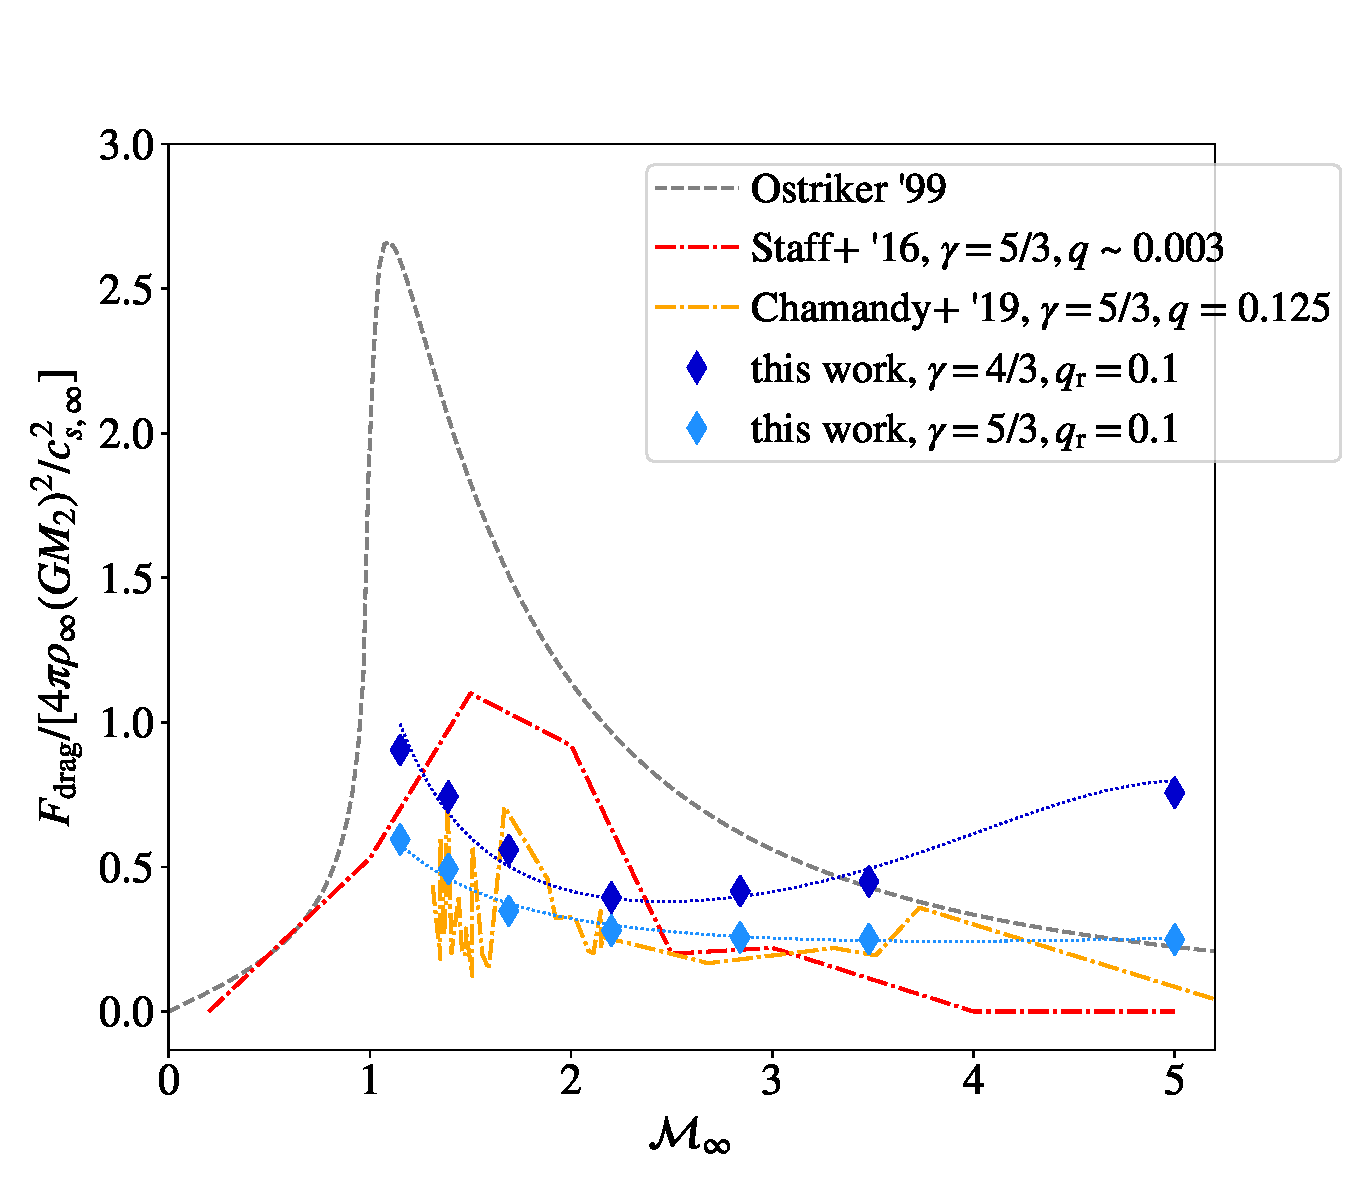
\includegraphics[width=13cm]{figures/common_envelope/Cd_ostriker_staff_chamandy_compare_ostriker_fig3units.pdf}\caption{Comparison of the evolution of drag forces with upstream Mach number obtained from ``wind-tunnel'' simulations in this work with other efforts to estimate drag forces applicable to common envelope (CE) interactions. Plotted are drag force estimates (i) on a massive perturber in a gaseous medium, derived analytically in Ref. \cite{1999ApJ...513..252O}, (ii) from global simulations in Ref. \cite{Staff:2016} modeling a CE interaction with binary mass ratio $q~\approx 0.003$, gas adiabatic index $\gamma = 5/3$, (iii) from global simulations in Ref. \cite{Chamandy:2019psk} modeling a CE interaction with binary mass ratio $q~\approx 0.125$, gas adiabatic index $\gamma = 5/3$, and (iv) from local simulations in this work modeling the CE dynamical inspiral phase with binary mass ratio $q~\approx 0.1$, gas adiabatic indices $\gamma = 4/3$ and $\gamma = 5/3$. \label{fig:drag_compare}}.
\end{figure*}
\Chapter{Igniting weak interactions in neutron-star post-merger accretion disks}
\label{ch:kilonova}

\section{Introduction}\label{sec:intro}

The gravitational-wave observatories advanced LIGO and Virgo, recently joined by KAGRA, are starting to make routine detections of compact binary mergers \cite{LIGOScientific:2018mvr,LIGOScientific:2020stg,Abbott:2020uma}\footnote{\href{https://gracedb.ligo.org/superevents/public/O3/}{https://gracedb.ligo.org/superevents/public/O3/}}. The first neutron-star (NS) merger GW170817 \cite{TheLIGOScientific:2017qsa} and a second NS merger candidate GW190425 \cite{Abbott:2020uma} already probe drastically different parts of the NS binary parameter space. While the component masses of GW170817 are typical of previously known Galactic double NS systems, the total mass of GW190425 of $\sim\!3.4\,M_\odot$---if indeed a double NS system---represents an outlier by $5\sigma$ with respect to the known Galactic distribution of binary NSs \cite{Abbott:2020uma} (or may represent a peculiar NS--BH or BH--BH system otherwise). Furthermore, while GW170817 was followed by electromagnetic counterparts across the entire electromagnetic spectrum \cite{abbott_multi-messenger_2017}, including the first unambiguous detection of a `kilonova' \cite{li_transient_1998-1,Kulkarni:2005jw,metzger_electromagnetic_2010,metzger_kilonovae_2019}, GW190425 did not lead to the detection of electromagnetic counterparts, which may be due to intrinsically dim emission, the large distance of $\sim\!160$\,Mpc to the binary, and poor sky localization of $\sim\!8,300\,\mathrm{deg}^2$ \cite{Abbott:2020uma,Antier:2019pzz,Hosseinzadeh:2019ifm,Coughlin:2019zqi}.

Six decades after Refs. \cite{burbidge_synthesis_1957-1} and \cite{cameron_origin_1957} realized that about half of the cosmic abundances of nuclei heavier than iron are created by rapid neutron capture onto light seed nuclei (`the r-process'), GW170817 provided the first direct observation of cosmic synthesis of such elements. The quasi-thermal emission in the ultraviolet, optical, and near-infrared was consistent with a kilonova, i.e., with being powered by the radioactive decay of r-process nuclei synthesized in the merger ejecta (see, e.g., \cite{metzger_kilonovae_2019,Siegel:2019mlp} for reviews discussing the interpretation of the event).

Binary NS or NS--BH mergers that lead to tidal disruption of the NS outside the innermost stable circular orbit can give rise to neutron-rich ejecta material conducive to the r-process in a number of ways. This includes dynamical ejecta with tidal and shock-heated components \cite{ruffert_coalescing_1997-1,rosswog_mass_1999,oechslin_relativistic_2007,hotokezaka_mass_2013,hotokezaka_progenitor_2013}, neutrino-driven and magnetically driven winds from a (meta-)stable remnant \cite{dessart_neutrino_2009,siegel_magnetically_2014,ciolfi_general_2017,ciolfi_first_2019}, and outflows from a post-merger accretion disk \cite{fernandez_delayed_2013,just_comprehensive_2015,siegel_three-dimensional_2017}. The details and relative importance of these ejecta components depend on binary parameters and the unknown equation of state (EOS) of nuclear matter at supranuclear densities (see Sec.~\ref{sec:intro_ignition_threshold} for more details). In particular, the bulk of the GW170817 ejecta, specifically the material giving rise to the `red' lanthanide-bearing kilonova component, is most naturally explained by outflows from a post-merger accretion disk \cite{Kasen:2017sxr,siegel_three-dimensional_2017}, while the origin of the `blue' emission in GW170817 may be due to a different source or combination of sources (\cite{siegel_three-dimensional_2018,fernandez_long-term_2019,miller_full_2019-1,nedora_spiral-wave_2019,metzger_magnetar_2018,Ciolfi:2020wfx}; see, e.g., \cite{metzger_kilonovae_2019} and \cite{Siegel:2019mlp} for more discussion). Due to issues with chemical evolution (see \cite{Siegel:2019mlp} for a brief summary) and the possibility of other sources such as magneto-rotational supernovae \cite{winteler_magnetorotationally_2012,halevi_r-process_2018} and collapsars \cite{siegel_collapsars_2019} contributing significantly, it still remains an open question whether NS mergers are the dominant source of r-process elements.

Post-merger accretion disks form as a significant amount of merger debris circularized around the remnant. Such disks also provide a promising central engine to generate collimated relativistic jets needed to generate short gamma-ray bursts \cite{aloy_relativistic_2005,shibata_merger_2006,paschalidis_relativistic_2015,ruiz_binary_2016}. Numerical studies of the evolution of such accretion disks exist with various levels of approximation and computational complexity \cite{fernandez_delayed_2013,just_comprehensive_2015,siegel_three-dimensional_2017,fernandez_long-term_2019,christie_role_2019,miller_full_2019-1,fujibayashi_properties_2017,Fujibayashi:2020qda}. Recent studies indicate that about 20--40\% of the disk material may be unbound into powerful neutron-rich outflows, which makes them a strong source of kilonova emission and a potentially dominant source of r-process ejecta across a wide region in NS binary parameter space (see Sec.~\ref{sec:intro_ignition_threshold} for a discussion). However, due to the computational complexity and cost, to date there exist only a few selected self-consistent simulations \cite{siegel_three-dimensional_2017,siegel_three-dimensional_2018,fernandez_long-term_2019,christie_role_2019,miller_full_2019-1} that take all necessary physical ingredients into account (see Secs.~\ref{sec:intro_ignition_threshold} and Sec.~\ref{sec:methods} for more details), and most of the post-merger parameter space and associated physics remains largely unexplored.

This paper presents the first exploration of the parameter space of neutrino-cooled accretion disks across two orders of magnitude in accretion rates and disk masses by means of self-consistent three-dimensional general-relativistic magnetohydrodynamic (GRMHD) simulations with weak interactions. This study is conducted in anticipation of future detections of binary mergers by LIGO, Virgo, and Kagra, which will in the next several years sample the NS merger parameter space with many more detections. This study focuses on the transition across an ignition threshold for weak interactions, which distinguishes qualitatively distinct states and properties of such accretion disks and related parts of the neutron star binary parameter space. We begin by elaborating on this ignition threshold (Sec.~\ref{sec:intro_ignition_threshold}) and by relating post-merger disks to NS binary parameters and future detections (Sec.~\ref{sec:param_space}). A brief overview of numerical methods is provided in Sec.~\ref{sec:methods}. Section \ref{sec:results} summarizes our results, including global and local disk properties as well as r-process nucleosynthesis. Discussion and conclusions are presented in Sec.~\ref{sec:conclusion}.

%Post-merger accretion disks have recently been shown to constitute a significant, if not dominant, source of ejecta and kilonova emission in NS mergers \cite{}. Mention early MHD vs. late viscous driven winds. Total outflow and thus overall composition dominated by early MHD winds \cite{}. Most of the accretion disk mass is accreted or evaporated into winds in this early phase. Composition and kilonova color mostly set by complex interplay between MHD turbulence and weak interactions in the first few hundred ms after merger.


\section{Physical model}

\subsection{NS post-merger disks: ignition threshold}
\label{sec:intro_ignition_threshold}

Compact accretion disks while optically thick to photons may be cooled via neutrino emission %, which affects the lepton number and thus the composition of the disk 
\cite{popham_hyperaccreting_1999,narayan_accretion_2001-1,di_matteo_neutrino_2002,beloborodov_nuclear_2003,kohri_neutrino-dominated_2005,chen_neutrino-cooled_2007,kawanaka_neutrino-cooled_2007}. At sufficiently high midplane density and temperature, weak interaction rates become high relative to the rate of radial advection of thermal energy. This gives rise to two limiting states of such disks: $(i)$ weak interactions are important and the disk is neutrino-cooled (predominantly via electron and positron capture: $e^- + p \rightarrow n + \nu_e$, $e^+ + n \rightarrow p + \bar{\nu}_e$); $(ii)$ weak interactions and neutrino cooling are negligible. In addition to changing the thermodynamics, weak interactions also change the lepton number and thus the composition of the disk and its outflows. The composition in stationary state as parametrized by the electron fraction $Y_e= n_{\rm p}/n_{\rm b}$, with $n_{\rm p}$ and $n_{\rm b}$ denoting the proton and total baryon number densities, is determined by the degree of electron/positron degeneracy \cite{beloborodov_nuclear_2003,chen_neutrino-cooled_2007,siegel_three-dimensional_2017,siegel_three-dimensional_2018}, which we explore further in this paper (Sec.~\ref{sec:disk_composition}). This has important consequences for r-process nucleosynthesis and the nature of the associated kilonova emission (Sec.~\ref{sec:nucleosynthesis}).

Weak interactions are expected to become important above a certain `ignition' threshold on the accretion rate \cite{chen_neutrino-cooled_2007,metzger_time-dependent_2008},
\begin{eqnarray}
    \dot{M}_{\rm ign} &\approx& \dot{\mathcal{M}}_{\rm ign}(M_{\rm BH},\chi_{\rm BH})\alpha_{\rm visc}^{\frac{5}{3}} \label{eq:Mdot_ign}\\ 
    &\approx& 2\times 10^{-3} M_\odot \,\text{s}^{-1} \left(\frac{\alpha_{\rm visc}}{0.02}\right)^{\frac{5}{3}} \label{eq:Mdot_ign_merger}.  
\end{eqnarray}
In the second step, we have evaluated the expression for the regime of post-merger disks, assuming a black-hole of mass $M_{\rm BH}=3M_\odot$ and dimensionless spin of $\chi_{\rm BH}\approx 0.8$ (see Sec.~\ref{sec:methods}) and normalizing to a dimensionless Shakura-Sunyaev viscosity coefficient $\alpha_{\rm visc} = 0.02$ (see Sec.~\ref{sec:viscosity}). While this relation has been found numerically for 1D disk solutions in Kerr spacetime \cite{chen_neutrino-cooled_2007}, we show here that the scaling $\dot{M}\propto \alpha_{\rm visc}^{5/3}$ can be obtained analytically (see Appendix \ref{app:ignition_threshold}). Essentially, the ignition threshold can be written as a condition on the accretion rate as a result of the fact that viscous heating, neutrino cooling, and accretion rate scale with the midplane density (see Appendix \ref{app:ignition_threshold}).

Many previous simulations have been performed in hydrodynamics adopting $\alpha_{\rm visc}$ as a parameter \cite{fernandez_delayed_2013,fernandez_outflows_2015,just_comprehensive_2015,fujibayashi_properties_2017,Fujibayashi:2020qda}, some of which additionally approximate GR effects by a pseudo-Newtonian potential. While such $\alpha$-disk models are able to qualitatively capture the evolution of disk density and angular momentum, the nature of turbulence (convection) is fundamentally different from self-consistent magnetohydrodynamic turbulence driven by the magnetorotational instability (MRI; \cite{hawley_powerful_1992,balbus_nature_2002}). MHD disks self-consistently set an effective  $\alpha_{\rm visc}$ and thus self-consistently control the relative importance of weak interactions to viscous energy transport\footnote{This is only true in three spatial dimensions, as the anti-dynamo theorem in axisymmetry \cite{cowling_magnetic_1933} does not allow for a steady turbulent state.}; this, in turn, sets the composition of disk and outflow material and thus determines the nucleosynthetic r-process yields and kilonova colors to which such disks give rise. Furthermore, while $\alpha$-disks dissipate heat generated by viscosity locally and predominantly in the disk midplane (proportional to the gas density), MHD disks dissipate a significant fraction non-locally via reconnection in low-density regions of a disk corona \cite{jiang_global_2014,siegel_three-dimensional_2018}. This difference is crucial in launching outflows, which originate from the `hot' corona with the additional help of free nuclei recombining into $\alpha$ particles \cite{siegel_three-dimensional_2018}. Indeed, a careful comparison between a post-merger GRMHD and $\alpha$-disk simulation shows that MHD disks are much more effective in evaporating material early on, giving rise to most of their ejecta mass during the first few hundred milliseconds, before viscous spreading (as in an $\alpha$-disk) takes over \cite{fernandez_long-term_2019}. This leads to the preliminary conclusion that MHD disks can eject up to 30-40\% of their initial disk mass \cite{siegel_three-dimensional_2018,fernandez_long-term_2019}, which we shall investigate further in this paper (Sec.~\ref{sec:ejecta}).

\subsection{NS post-merger disks: relation to binary parameters}\label{sec:param_space}

Figures \ref{fig:bns_parameters} and \ref{fig:nsbh_parameters} show mappings between binary parameters, accretion disk masses, and ejecta masses (dynamical and disk ejecta) for plausible binary neutron star (BNS) and neutron star black hole (NSBH) systems. Mappings from binary parameters to BNS disk masses, BNS dynamical ejecta, and NSBH dynamical ejecta are based on fitting formulae to numerical relativity simulations as considered by Ref. \cite{kruger_2020} for the respective cases. Mapping the binary parameters to NSBH disk masses is based on the fitting formula provided by Ref. \cite{foucart_remnant_2018}. White lines in Figs.~\ref{fig:bns_parameters} and \ref{fig:nsbh_parameters} indicate the disk models simulated here, highlighting the regime of parameter space we focus on in this work.

For BNS systems, Ref. \cite{kruger_2020} find that disk masses extracted from existing BNS simulations can be fit to $\sim35\%$ accuracy by a formula of the type $M_{\rm disk}=M_2[aC_2 +c]^d$, which is effectively insensitive to mass ratio to leading order. Disk masses scale with the mass and compactness of the secondary (lighter) neutron star $C_2 = GM_2/(R_2c^2)$, and thus increase with stiffer EOSs and smaller secondary component masses. For small total mass BNS systems (middle panel of Fig.~\ref{fig:bns_parameters}), mergers give rise to both dynamical ejecta and disk ejecta, irrespective of the stiffness of the EOS, while for high total mass systems (right panel of Fig.~\ref{fig:bns_parameters}) both disk masses and the amount of dynamical ejecta are reduced or even non-existent due to the fact that the BNS quickly collapse to a black hole after merger and little to no material is left outside the event horizon. 

\begin{landscape}
\begin{figure}[t]
  \centering
  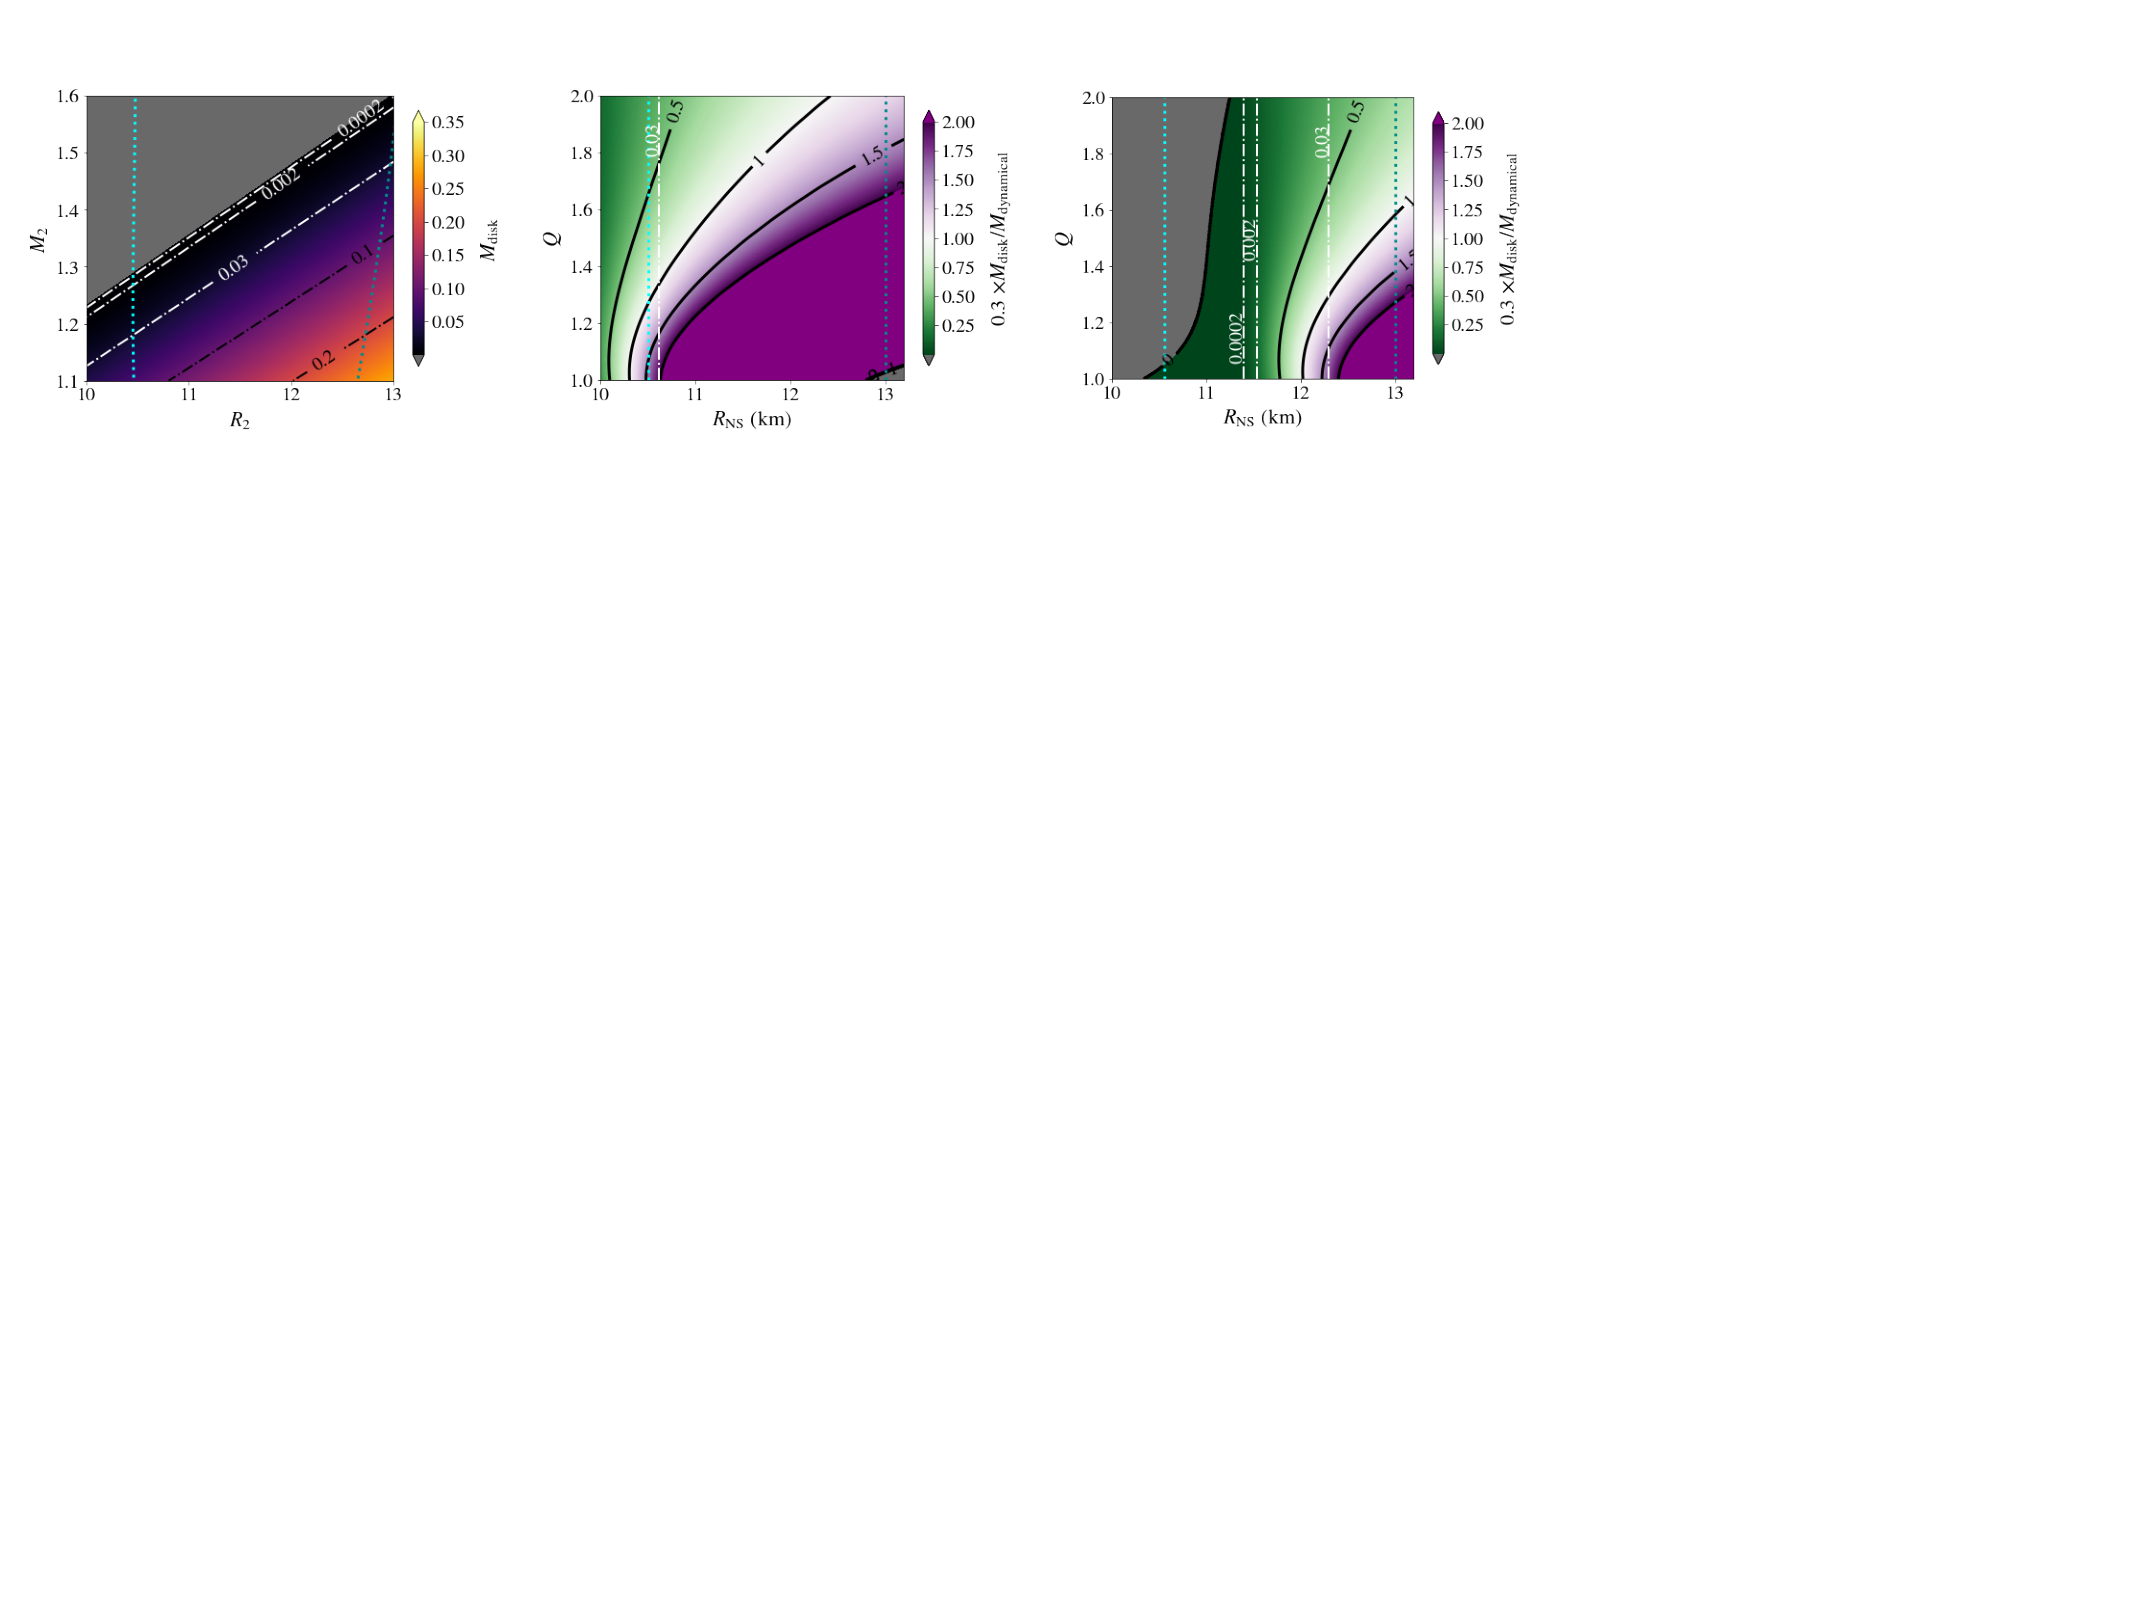
\includegraphics[width=22cm]{figures/kilonova/BNS_parameters_plot.pdf}
\caption{Approximate mapping between binary parameters and accretion disk as well as ejecta masses for binary neutron star systems. Left: Disk mass as a function of mass and radius of the secondary (less-massive) neutron star. Middle: Ratio of disk to dynamical ejecta as a function of the binary mass ratio ($Q = M_1/M_2$) and radius of the component neutron stars (assuming both stars have roughly the same radius), with the mass of the secondary fixed to $M_2 = 1.2~M_\odot$ and assuming disk ejecta to be 30\% of the initial disk mass. Right: Same as the middle panel, but for $M_2 = 1.4~M_\odot$. The dot-dashed lines (in white) delineate the disk masses $M_{\rm disk} = 0.03~M_\odot$, $0.002~M_\odot$, $0.0002~M_\odot$ considered for post-merger simulations in this work. Dotted lines (in cyan) show the lower and upper limits of neutron star radii allowed by recent observations~\cite{De:2018uhw,capano_stringent_2020,Miller:2019cac,Riley:2019yda,Landry:2020vaw}.\label{fig:bns_parameters}}
\vspace{5mm}
\end{figure}
\end{landscape}

\begin{landscape}
\begin{figure*}[t]
  \centering
  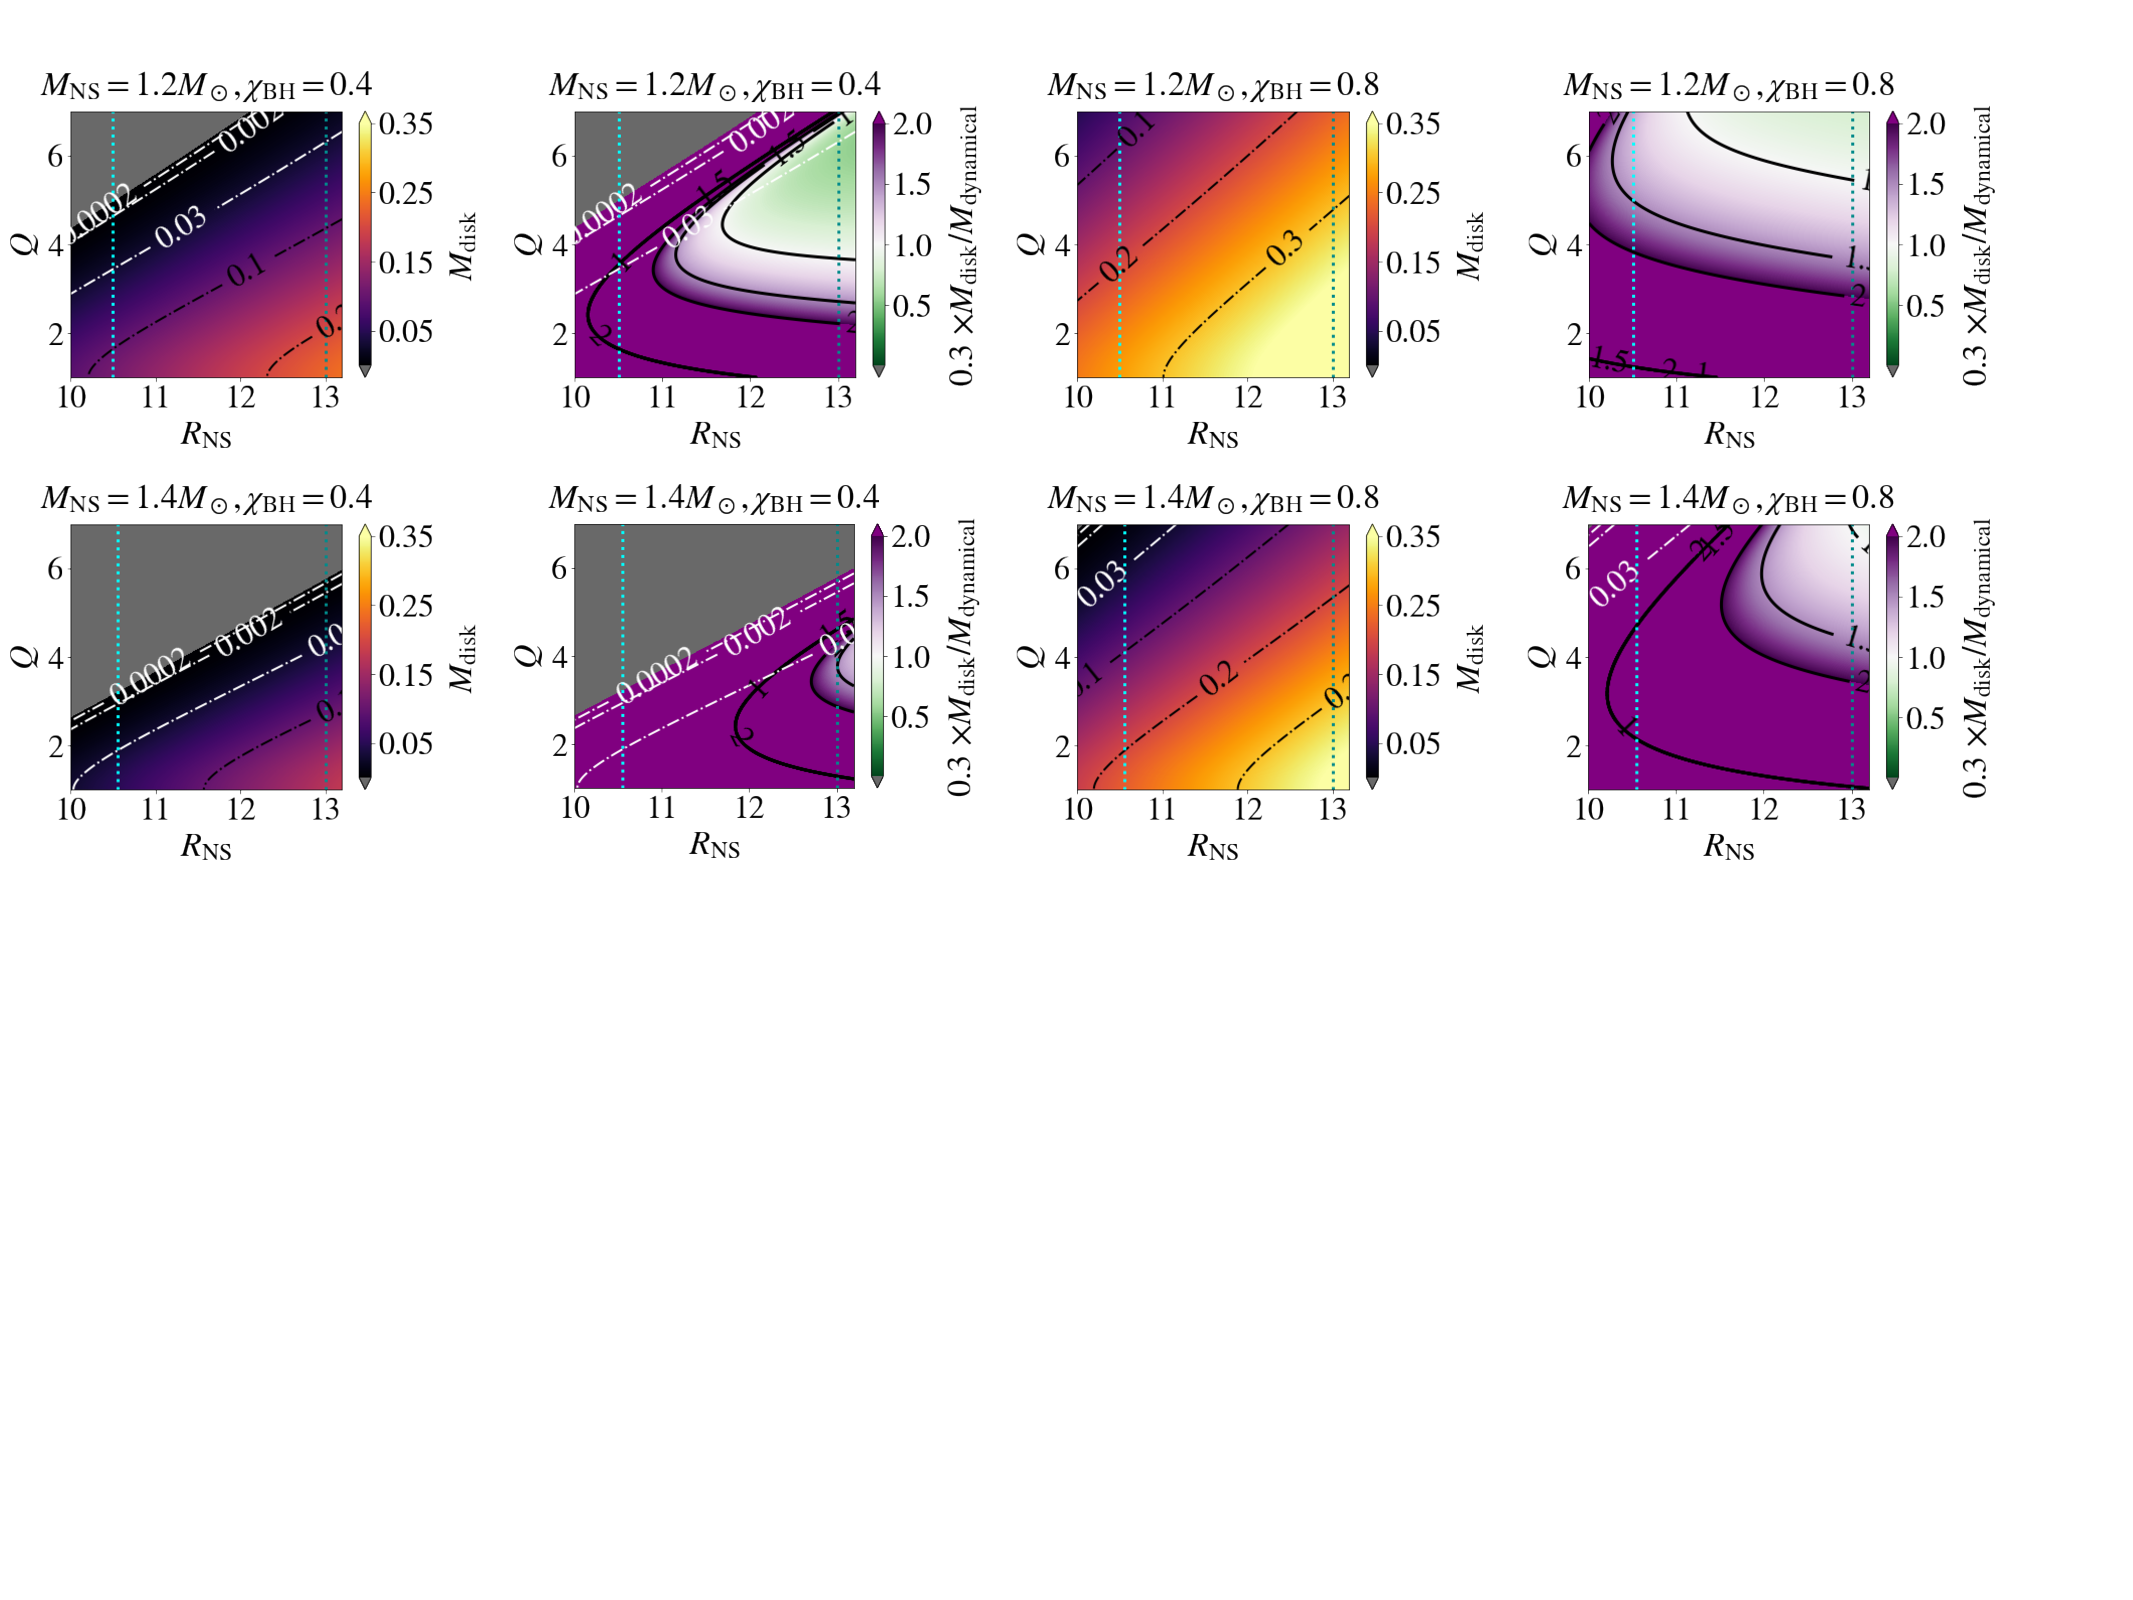
\includegraphics[width=22cm]{figures/kilonova/NSBH_parameters_plot.pdf}
 \caption{Approximate mapping between binary parameters and accretion disk as well as ejecta masses for neutron star-black hole binary systems. Shown are post-merger disk masses and ratios of disk to dynamical ejecta (assuming disk ejecta to be 30\% of the initial disk masses) as a function of the NS radius and the binary mass ratio $Q = M_{\rm BH}/M_{\rm NS}$ for different scenarios, including light and heavier NSs ($M_{\rm NS} = 1.2M_\odot,\, 1.4M_\odot$) and slowly or rapidly spinning BHs (dimensionless spin 0.4 or 0.8). The dot-dashed lines (in white) indicate the disk masses $M_{\rm disk} = 0.03~M_\odot$, $0.002~M_\odot$, $0.0002~M_\odot$ considered for the simulations in this work. Dotted lines (in cyan) show the lower and upper limits of neutron star radii allowed by observations as in Fig.~\ref{fig:bns_parameters}.\label{fig:nsbh_parameters}}
\vspace{5mm}
\end{figure*}
\end{landscape}

Both the binary mass ratio and the EOS determine the dominant source of ejecta in BNS mergers. Disk ejecta dominates over dynamical ejecta across most of the parameter space for small total-mass systems (middle panel of Fig.~\ref{fig:bns_parameters}), except for very small NS radii $\lesssim\!10.5$\,km and large mass ratios $Q\gtrsim 1.6$, while dynamical ejecta dominates in high total-mass systems (right panel of Fig.~\ref{fig:bns_parameters}), unless for larger NS radii $\gtrsim\!12$\,km and small-to-medium mass ratios $Q\lesssim 1.4$. For low-mass BNS systems, the disks simulated here cover the parameter space for small NS radii $\lesssim\!11$\,km, while for high-mass systems they span a wide range of $11\lesssim R_{\rm NS}\lesssim 12.5$\,km. We note that the results of our highest-$M_{\rm disk}$ run can be qualitatively extrapolated to larger disk masses and thus cover most of the remaining parameter space; however, for very massive disks effects of self-irradiation of the outflows become increasingly significant, leading to a more pronounced tail of `blue' ejecta \cite{miller_full_2019-1}. Depending on the secondary mass, the disk outflows of our simulated models may or may not dominate the total ejecta from the system.

In NSBH systems, dynamical ejecta and post-merger accretion disks only arise if the NS is tidally disrupted by the BH. This disruption process requires the tidal disruption radius to reside outside of the innermost stable circular orbit of the BH, and it thus depends on the spin $\chi_{\rm BH}$ of the BH and its mass (and thus on the mass ratio $Q = M_{\rm BH}/M_{\rm NS}$ of the binary). Ouflows from accretion disks typically dominate across most of the parameter space (cf.~Fig.~\ref{fig:nsbh_parameters}, except for light NSs (~$1.2M_\odot$) with large NS radii $\gtrsim 11.5$\,km and medium-to-large mass ratios $Q\gtrsim 3-4$, somewhat dependent on the BH spin.

In the NSBH parameter space, our models simulated here reside in the unequal mass ratio, low BH-spin regimes. Disk ejecta is dominant in this regime, and dynamical ejecta is absent.

%In the NSBH parameter space, our models lie in the unequal mass ratio, low spin regimes. Disk ejecta is dominant in this regime, and dynamical ejecta is absent.

%In the BNS parameter space, our models correspond to low total mass with soft equation of state merger scenarios, or high total mass with stiff equation of state scenarios. \texttt{MD\_M03} covers the regime where disk mass ejecta is dominant or subdominant, whereas \texttt{MD\_M002} and \texttt{MD\_M0002} cover the regime where dynamical ejecta is dominant.



\section{Numerical Methods}
\label{sec:methods}

%comment on grid setup (box sizes, resolution etc.)
\subsection{Simulation setup}\label{subsec:sim_setup}
We perform simulations in ideal GRMHD and full 3D with a fixed background spacetime for computational efficiency using the code and numerical setup described in Ref. \cite{Siegel:2017jug}. The code is based on \texttt{GRHydro}~\cite{mosta_grhydro:_2014} and makes use of the \texttt{Einstein Toolkit}\footnote{\href{http://einsteintoolkit.org}{http://einsteintoolkit.org}} \cite{maria_babiuc_hamilton_2019_3522086,loffler_einstein_2012,Schnetter:2003rb,Goodale:2002a,Thornburg:2003sf}, with neutrino interactions implemented via a leakage scheme based on Refs. \cite{Bruenn:1985en} and \cite{ruffert_coalescing_1996}, and follows the implementation of Refs. \cite{galeazzi_implementation_2013} and \cite{radice_dynamical_2016}. Thermodynamic properties of matter are based on the Helmholtz EOS \cite{timmes_accuracy_1999,timmes_accuracy_2000}, and we compute abundances of nuclei at a given density, temperature, and electron fraction $Y_e$, assuming nuclear statistical equilibrium.

The simulations include a Kerr black hole of mass $3.0 M_\odot$ and dimensionless spin $\chi_{\rm BH} = 0.8$, initially surrounded by a torus of constant specific angular momentum, small constant specific entropy of $8~k_{\rm B}$ per baryon, and initial electron fraction $Y_{\rm e} = 0.1$; we refer to Table \ref{tab:ini_config_torus} for a summary of initial torus properties of simulation runs. Run \texttt{MD\_M03} has been discussed before \cite{siegel_three-dimensional_2017,Siegel:2017jug}, and is further elaborated on here by comparing it to the two new runs \texttt{MD\_M002} and \texttt{MD\_M0002}, which represent lighter accretion disks. The BH-disk problem is formulated in Cartesian, horizon-penetrating Kerr-Schild coordinates. The black-hole mass and spin reflect typical NS merger scenarios (see Sec.~\ref{sec:param_space}). The black hole spins in the case of prompt black hole formation from BNS mergers are typically not larger than $\chi_{\rm BH} \approx 0.8$~\cite{kiuchi_longterm_2009,rezzolla_accurate_2010,bernuzzi_mergers_2014,kastaun_black_2013}, and black hole spins in case of delayed black hole formation are $\chi_{\rm BH} \lesssim 0.7$ \cite{sekiguchi_dynamical_2016}. Furthermore, $\chi_{\rm BH} \sim 0.8$ is significant enough to disrupt the NS and lead to a post-merger accretion disk in NSBH mergers across a wide range in mass ratio (\cite{foucart_black-hole-neutron-star_2012}; see the discussion in Sec.~\ref{sec:param_space}). Our initial tori masses are chosen to reflect a mass range covering the ignition threshold for weak interactions in post-merger disks (cf.~Sec.~\ref{sec:intro_ignition_threshold}) and is typical both for BNS and NSBH scenarios (Sec.~\ref{sec:param_space}).

\begin{table*}
\caption{Initial configurations of the accretion disks simulated here. From left to right: black-hole mass and dimensionless spin, disk mass, inner and outer radius of the disk, radius at maximum density, specific entropy, electron fraction, and maximum magnetic-to-fluid pressure ratio.}
\begin{centering}
\begin{tabular}{cccccccccc}
\hline
Run  & $M_{\rm BH}$ & $a_{\rm BH}$ & $M_{\rm d,0}$ & $R_{\rm in,0}$ & $R_{\rm out,0}$  & $R_0$ & $s_0$ & $Y_{\rm e,0}$ & $p_b/p_{\rm f}$\\
& [$M_{\odot}$] & & [$M_{\odot}$] & [$M_{\rm BH}$] & [$M_{\rm BH}$] &  [km] & [$k_B$/b] & & \\
\hline 
MD\_03 & 3 & 0.8 & 0.03 & 4 & 24 & 30 & 8 & 0.1 & $< 5\times 10^{-3}$ \\
MD\_002 & 3 & 0.8 & 0.002 & 7 & 20 & 45.61 & 8 & 0.1 & $< 5\times 10^{-3}$ \\
MD\_0002 & 3 & 0.8 & 0.0002 & 12 & 20 & 66.27 & 8 & 0.1 & $< 5\times 10^{-3}$ \\
\hline 
\end{tabular}
\par\end{centering}
\label{tab:ini_config_torus}
\end{table*}

The tori are initialized with weak poloidal magnetic seed fields, confined to the interior of the tori and defined by the magnetic vector potential $A^r = A^{\theta} = 0$ and $A^{\phi} = A_b$ max$\{p - p_{\rm cut}, 0\}$. Here, $p$ denotes the fluid pressure, $p_{\rm cut}$ is the pressure below which the magnetic field is set to zero, and $A_b$ sets the initial field strength. Here, $p_{\rm cut} \approx 1\times 10^{-2} p_{\rm max}$ in all cases, where $p_{\rm max}$ is the pressure at maximum density in the torus. We choose $p_{\rm cut}$ such that the magnetic field covers the bulk volume of the torus, while preventing it from becoming buoyant in the outermost layers and violently breaking out of the torus at the start of the simulation. We adjust $A_b$ such that the magnetic-to-fluid pressure ratio in the torus is a small value, $p_{\rm B}/p_{\rm f} < 5\times 10^{-3}$.

The initial torus is embedded in a tenuous atmosphere with $T = 10^5$ K, and $Y_{\rm e} = 1$ and $\rho \approx$ 37 g cm$^{-3}$, $\rho \approx$ 3.7 g cm$^{-3}$, and $\rho \approx$ 0.37 g cm$^{-3}$ for runs \texttt{MD\_M03}, \texttt{MD\_M002}, and \texttt{MD\_M0002}, respectively. The density and temperature are chosen such that they are sufficiently low to neither impact the dynamics nor the composition of the disk outflows. The atmosphere densities are set to approximately scale with the maximum density of the accretion disk during the evolution (cf.~Tab.~\ref{tab:torusenergytab}). The total atmosphere mass of the entire computational domain is $3.8\times 10^{-5} M_\odot$ for \texttt{MD\_M03}, $3\times 10^{-7} M_\odot$ for \texttt{MD\_M002}, and $3\times 10^{-8}$ for \texttt{MD\_M0002}, orders of magnitude smaller than the disk ejecta (cf.~Tab.~\ref{tab:torusenergytab}); over a volume of radius 1000\,km, which we consider as the minimum radius for outflow material to be unbound from the BH-disk system, the corresponding atmosphere masses are $1.8\times 10^{-8} M_\odot$ for \texttt{MD\_M03}, $1.8\times 10^{-9} M_\odot$ for \texttt{MD\_M002}, and $1.8\times 10^{-8} M_\odot$ for \texttt{MD\_M0002}). At the chosen atmosphere temperature of $T = 10^5$\,K weak interations are frozen out.

The computational domain represents a Cartesian grid hierarchy centered around the black hole. The grid has eight refinement levels, with an extent in each coordinate direction of $1.53\times 10^4$ km for \texttt{MD\_M03}, and $1.14\times 10^4$ km for \texttt{MD\_M002} and \texttt{MD\_M0002}. The initial tori have diameters of 240~km, 206~km, and 206~km for simulations \texttt{MD\_M03}, \texttt{MD\_M002}, and \texttt{MD\_M0002}, respectively. The initial tori are encompassed by the finest refinement level of the corresponding grid hierarchy. Following previous work \cite{siegel_magnetorotational_2013,Siegel:2017jug,siegel_collapsars_2019}, the finest resolution is $\Delta_{xyz} \approx 850$\,m for all simulations, chosen such that the MRI is well resolved in the stationary turbulent state of the disk (typically by ten grid points per fastest-growing MRI mode), which ensures convergence of global observables (see, e.g., \cite{siegel_collapsars_2019}).

Angular momentum transport is mediated by magnetic turbulence, driven by the MRI, in our setups. The initial tori undergo a relaxation phase with self-consistent magnetic-field amplification, and settle into a quasi-stationary phase at $\sim\!20$ ms. We consider the relaxed state of the disks at this time as the actual initial data for our simulations, and exclude the early transient phase from our analysis---in particular, the small amount of material accreted onto the black hole or ejected via outflows during this phase.

\subsection{Diagnostics}\label{subsec:diagnostics}

In order to monitor certain physical quantities in the disk, we compute radial profiles of such a quantity $\chi(\varpi)$ by performing azimuthal, density-weighted averages, integrating up to one scale height of the disk (see Equation \ref{eq:scale_ht} below for the definition of the scale height):
%Azimuthal averages of a quantity $\chi$ are defined as
%\begin{equation}
%    \langle \chi \rangle_\phi = \frac{\int^{2\pi}_{0} \chi \sqrt{\gamma_{\phi \phi}}d\phi}{\int^{2\pi}_{0} \sqrt{\gamma_{\phi \phi}}d\phi}
%\end{equation}
%where $\gamma_{ij}$ are the spatial components of the metric tensor $g_{\mu\nu}$ in 3+1-split. We define density-weighted averages 
\begin{equation}\label{eq:radial_av}
    \langle \chi \rangle_{{\rm azim}, z_H} = \frac{\int^{z_H}_{-z_H} \int_0^{2\pi} \chi \hat D \varpi d\phi dz}{\int^{z_H}_{-z_H} \int_0^{2\pi} \hat D \varpi d\phi dz}.
\end{equation}
Here, $\varpi = \sqrt{x^2 + y^2}$ is the cylindrical radius, $\hat D = \sqrt{\gamma} \rho W$ is the conserved rest-mass density as seen by the Eulerian observer moving normal to the spatial hypersurfaces in the 3+1 split of Kerr-Schild spacetime, $\gamma$ here is the determinant of the spatial metric $\gamma_{ij}$ in 3+1 split, and $W$ the Lorentz factor of the fluid. The density scale height $z_H$ is defined as
\begin{equation}\label{eq:scale_ht}
    z_H (\varpi) = \frac{\int \int_0^{2\pi} |z| \hat D \varpi d\phi dz}{\int \int_0^{2\pi}\hat D \varpi d\phi dz}.
\end{equation}
By integrating up to the local density scale height, we exclude the disk corona and winds from the calculation. For some quantities, temporal averages $\langle\cdot\rangle_t$ (cf., eg., Eqs.~\eqref{eq:alpha_visc_def_1D} and \eqref{eq:alpha_visc_def_0D}) over a specified time window are taken, in order to reduce the effect of temporal fluctuations of a turbulent medium.

For some disk quantities, it is useful to compute the rest-mass density average and study its evolution over time. We define this averaging as
\begin{equation}\label{eq:rest_mass_dens}
 \langle \chi \rangle_{\hat D} = \frac{\int \chi \hat D d^3x}{\int \hat D d^3x}.
\end{equation}
In some cases, this average is calculated by integrating only up to the local scale height,
\begin{equation}\label{eq:rest_mass_dens_scaleht}
    \langle \chi \rangle_{\hat D, z_H} = \frac{\int^{z_H}_{-z_H} \chi \hat D \varpi dz}{\int^{z_H}_{-z_H} \hat D \varpi dz},
\end{equation}
which allows us to explicitly exclude the disk corona and disk wind regions.


\section{Numerical Results}
\label{sec:results}

We proceed by first discussing our results for global disk properties, such as MHD mediated angular momentum transport (Sec.~\ref{sec:viscosity}), accretion (Sec.~\ref{sec:accretion}), neutrino emission (Sec.~\ref{sec:neutrino_emission}), disk ejecta (Sec.~\ref{sec:ejecta}), before discussing disk evolution locally in terms of weak interactions (Sec.~\ref{sec:disk_composition}) and nucleosynthesis from the disk outflows (Sec.~\ref{sec:nucleosynthesis}).


\subsection{Global properties}
\label{sec:global_properties}

\begin{table*}
\caption{Various properties of the accretion disks simulated here. From left to right: average density, and accretion rate after relaxation, estimated total unbound disk outflow mass ($M_{\rm ej}$; `ejecta') in solar masses and in units of the total disk mass ($M_{\rm tot}$) after relaxation, with mean electron fraction, initial total neutrino luminosity in electron and anti-electron neutrinos, effective $\alpha$-viscosity parameter, viscous evolution time and total evolution time for the respective runs. The averages $\bar{\rho}_{\rm d}$ and $\bar \alpha_\mathrm{vis}$ with the quoted uncertainties represent density-weighted average, maximum, and minimum values around a 10\,ms window centered at $t = 30$\,ms (see the text for details). The values for $\dot{M}_{d}$ with quoted uncertainties represent the average, maximum, and minimum values over the same time window at $t = 30$\,ms. The values for $L_{\nu,\mathrm{max}}$ represent the average value extracted from the neutrino luminosity over a 10\,ms window centered at the global peak luminosity of anti-electron neutrinos.
}
\setlength{\tabcolsep}{5pt}
\begin{centering}
\begin{adjustwidth}{-1.25cm}{}
{\normalsize\renewcommand{\arraystretch}{.8}
\resizebox{!}{.045\paperheight}{%
\begin{tabular}{cccccccccc}
\hline
Run  & $\bar{\rho}_{\rm d}$ & $\dot{M}_{d}$  & $M_{\rm ej}$ & $M_{\rm ej}/M_{\rm tot}$ & $\bar{Y}_e$ & $L_{\nu,\mathrm{max}}$ & $\bar \alpha_\mathrm{vis}$ & $t_{\rm visc}$ & $t_{\rm end}$\\
 & [$\mathrm{g}\,\mathrm{cm}^{-3}$] & [$M_{\odot}\,\mathrm{s}^{-1}$] &  [$M_{\odot}$] & & & [$\mathrm{erg}\,\mathrm{s}^{-1}$] & & [ms] & [ms]\\
\hline 
MD\_03 & $5.53_{-1.4}^{+2.2}\times 10^{10}$ & $2.6_{-0.7}^{+1.4}\times 10^{-1}$ & $3.179\times 10^{-3}$ & 0.157 & 0.174 & 2.1$\times 10^{52}$ & $1.76_{-1.7}^{+2.8}\times 10^{-2}$ & 279 & 381\\
MD\_002 & $6.6^{+0.5}_{-0.9}\times 10^9$ & $1.14_{-0.4}^{+0.4}\times 10^{-2}$ & $4.030\times 10^{-4}$ & 0.171 & 0.114 & 14$\times 10^{50}$ & $1.01_{-0.6}^{+1.5}\times 10^{-2}$ & 874 & 309\\
MD\_0002 & $3.4^{+0.7}_{-0.6}\times 10^8$ & $3.79_{-1.7}^{+2.5}\times 10^{-4}$ & $6.046\times 10^{-5}$ & 0.356 & 0.101 & 2.1$\times 10^{48}$ & $1.14_{-1.1}^{+2.0}\times 10^{-2}$ & 1731 & 294\\
\hline 
\end{tabular}
}}
\end{adjustwidth}
\par\end{centering}
\label{tab:torusenergytab}
\end{table*}

\subsubsection{MHD turbulence \& effective viscosity}
\label{sec:viscosity}

%\textcolor{red}{note that amplification of B-filed and development of MHD turbulence self-consistent from much weaker fields as in previous papers. Discuss computation of effective alpha-viscosity parameter and include \& describe plot (similar as in collapsar paper). Remark that it's a constant among the simulations and in above equation, hence the scaling between Mdot and rho\_d.}

\begin{figure}[t]
\centering
  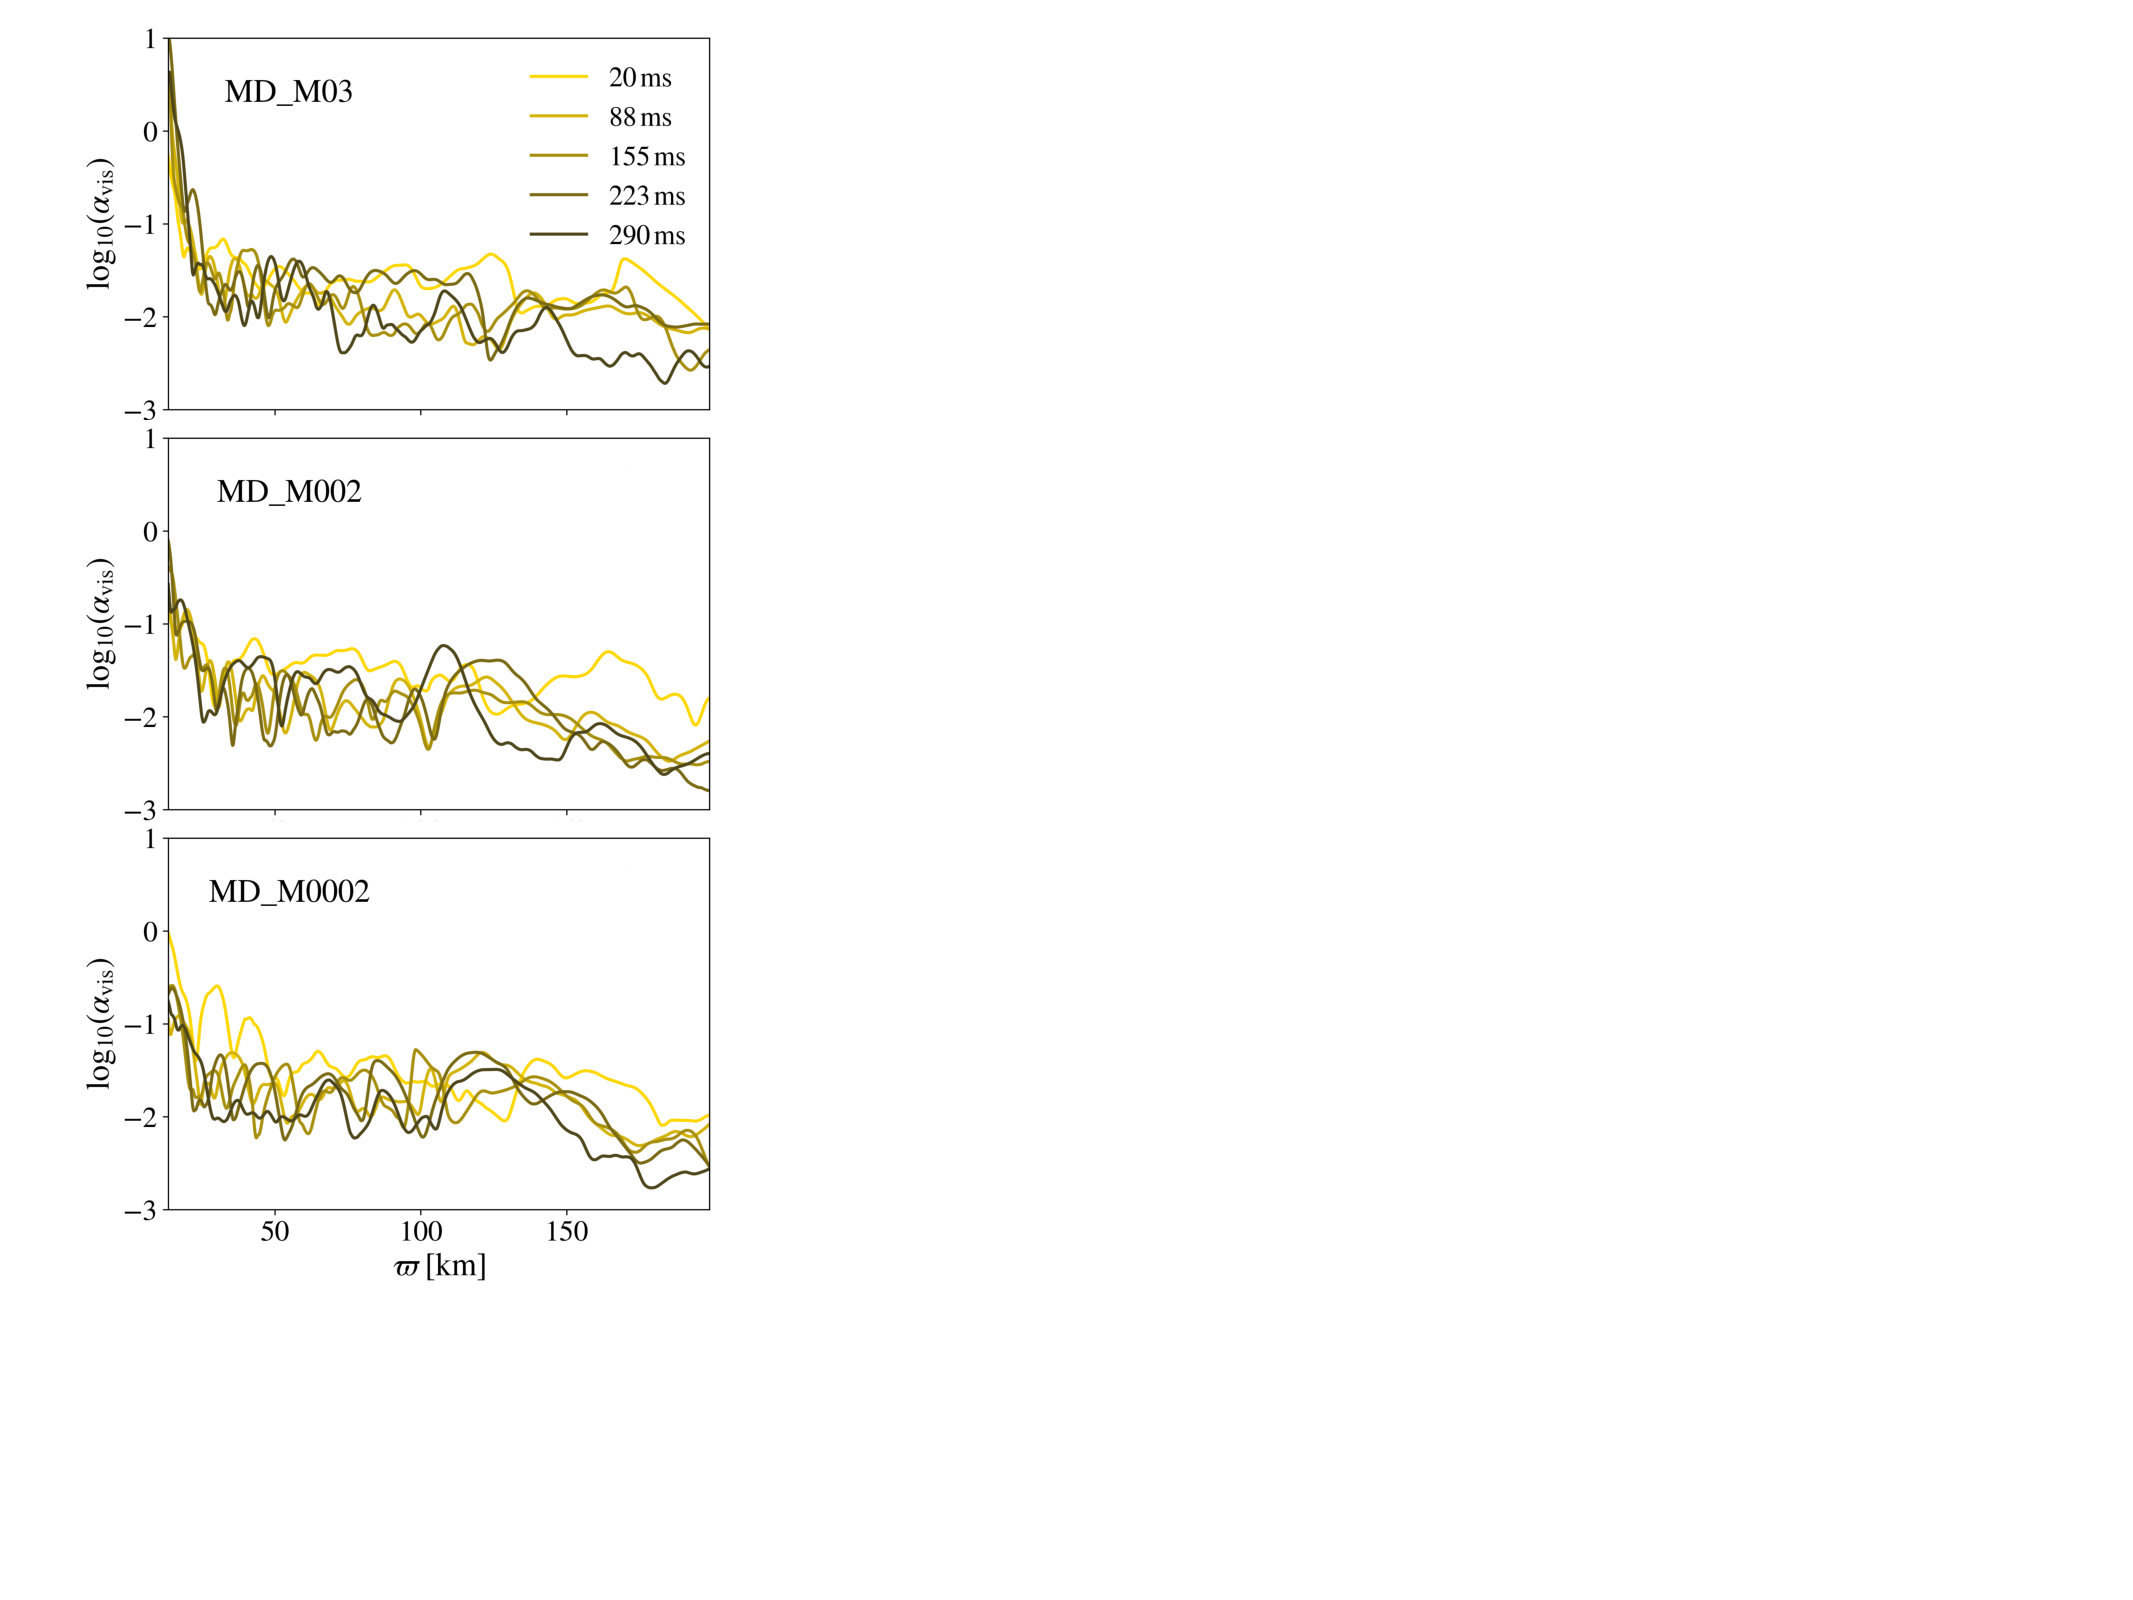
\includegraphics[width=10cm]{figures/kilonova/alpha-viscosity.pdf}
 \caption{Radial profiles of the effective Shakura-Sunyaev viscosity parameter $\alpha_{\rm vis}$ defined in Eq.~\eqref{eq:alpha_visc_def_0D} at different times during the evolution for the three simulation runs in this work. \label{fig:alpha-viscosity}}
\vspace{5mm}
\end{figure}

Soon after the start of the simulations, our accretion disks show vigorous magnetic turbulence, triggered by the MRI, a local fluid instability developed in differentially rotating magnetized fluids~\cite{velikhov_notitle_1959,chandrasekhar_stability_1960,balbus_powerful_1991,1998RvMP...70....1B,Balbus:2003xh,armitage_dynamics_2011}. The initial weak magnetic field in the simulations is purely poloidal, and it is amplified by the MRI at an exponential rate. As the simulation progresses, a toroidal field component is initially amplified by magnetic winding, before the toroidal field becomes susceptible to the MRI as well. This combination of the MRI and magnetic winding causes an overall increase of the maximum total magnetic field strength. At $t\approx 20$~ms, a steady turbulent state is achieved by the disk and the magnetic field, self-consistently amplified by the MRI, reaches saturation, loosing memory of the initial magnetic field configuration. We refer to Ref. \cite{siegel_three-dimensional_2018} for a more detailed discussion on how this turbulent state arises.

MHD turbulence in the disk operates as large-scale viscosity, which can be parameterized by an effective Shakura-Sunyaev viscosity $\alpha_{\rm vis}$. We define this quantity as
\begin{equation}
    \alpha_{\rm vis} (\varpi) = \frac{\langle \langle |T^{r,\phi}|\rangle_{{\rm azim}, z_H}\rangle_t}{\langle \langle p \rangle_{{\rm azim}, z_H}\rangle_t}, \label{eq:alpha_visc_def_0D}
\end{equation}
where $T^{r,\phi}$ is the $r-\phi$ component of the stress-energy tensor in the frame comoving with the fluid, and $p$ the fluid pressure. %Here, time averages are taken over a few neighboring data snapshots over a time-span of $\approx 10$~ms.

Figure \ref{fig:alpha-viscosity} shows radial profiles of $\alpha_{\rm vis}$, computed using Eq.~\eqref{eq:radial_av}, at different times during the disks' evolution, for all three simulation runs. We find that $\alpha_{\rm vis}$ is roughly constant among the simulations, independent of the initial disk mass. Table \ref{tab:torusenergytab} reports global values for $\alpha_{\rm vis}$ for each simulation. The latter values describe the accretion state of the inner disk. We compute these values as an average over a 10~ms time-window centered at $t = 30$~ms, extracted from the time evolution of the absolute value of the rest-mass density average of $\alpha_{\rm vis}$,
\begin{equation}
    \alpha_{\rm vis} = \frac{\langle \langle |T^{r,\phi}|\rangle_{\hat{D}, z_H}\rangle_t}{\langle \langle p \rangle_{\hat{D}, z_H}\rangle_t}. \label{eq:alpha_visc_def_1D}
\end{equation}
The rest-mass density average is calculated following the procedure in Equation \eqref{eq:rest_mass_dens_scaleht}, restricting to the region between 30-175\,km from the centers of the black holes. By applying this restriction along the radial extent, only the inner disk regions that can be directly related to the accretion rate onto the black hole are used in the calculation; the data of the outer parts of the disks that start to viscously spread are excluded from the calculation. Also excluded are the innermost regions that show a rise of $\alpha_\mathrm{eff}(\varpi)$ toward the innermost stable circular orbit and the black-hole horizon due to increasing mean magnetic field strengths (\cite{penna_shakura-sunyaev_2013}; cf.~Fig.~\ref{fig:alpha-viscosity}). As indicated by the radial profiles in Fig.~\ref{fig:alpha-viscosity}, the averages for $\alpha_{\rm vis}$ in the inner disks as reported in Tab.~\ref{tab:torusenergytab} are roughly constant among the different accretion disks explored here.

The extraction of effective $\alpha$-viscosities allows us to compute approximate viscous evolution timescales for our disks,
\begin{eqnarray}
	t_{\rm visc} &=& \frac{1}{\alpha}\left(\frac{R_0^{3}}{GM_{\rm BH}}\right)^{1/2}\left(\frac{z_H}{\varpi}\right)^{-2} \label{eq:tvisc} \\
	\approx&& \mskip-15mu 2.6\,{\rm s} \left( \frac{\alpha}{0.01}\right)^{-1}\mskip-5mu\left(\frac{R_0}{30\,{\rm km}}\right)^{\frac{3}{2}} \mskip-5mu\left(\frac{M_{\rm BH}}{3M_\odot}\right)^{-\frac{1}{2}} \mskip-5mu\left(\frac{z_H/\varpi}{0.1}\right)^{-2}\mskip-5mu, \nonumber
\end{eqnarray}
where we have normalized to typical values in our context in the second line. For further reference, viscous timescales for our simulation runs are listed in Tab.~\ref{tab:torusenergytab}. For all disks we find that the effective viscous timescales are typically of the order of a few seconds, and thus sufficiently long to explain the prompt emission of short gamma-ray bursts with typical durations of $T_{90}<2\,{\rm s}$ via accretion onto a black hole.

%This indicates that for a given $A(r)$, $M_{\rm BH}$, $H$, $r$, the scaling of $\dot M$ with $\bar{\rho}_{\rm d}$ always is a constant. $\dot M$ in the simulations is self-consistently set by MHD turbulence to obey this relation.




\subsubsection{Accretion}
\label{sec:accretion}

\begin{figure}[t]
  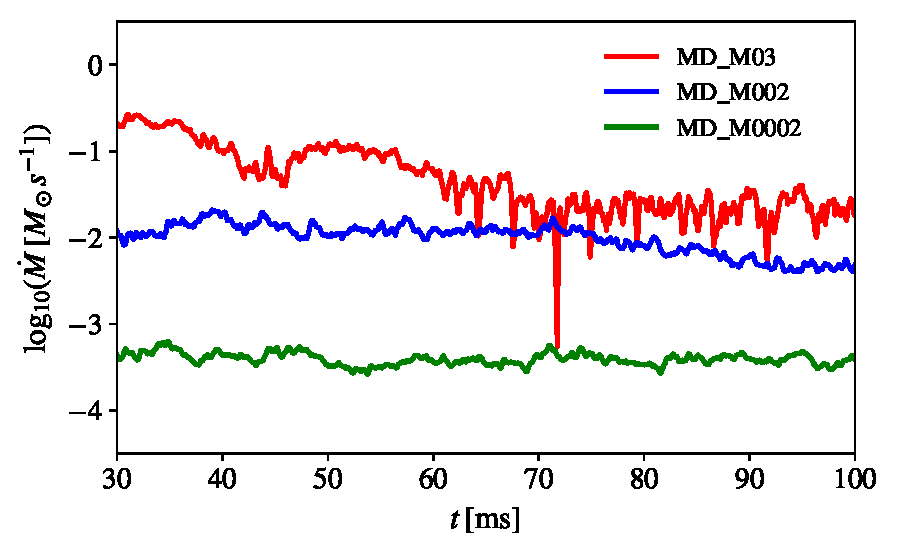
\includegraphics[width=\columnwidth]{figures/kilonova/Mdot_acc_multidets_sims.pdf}
  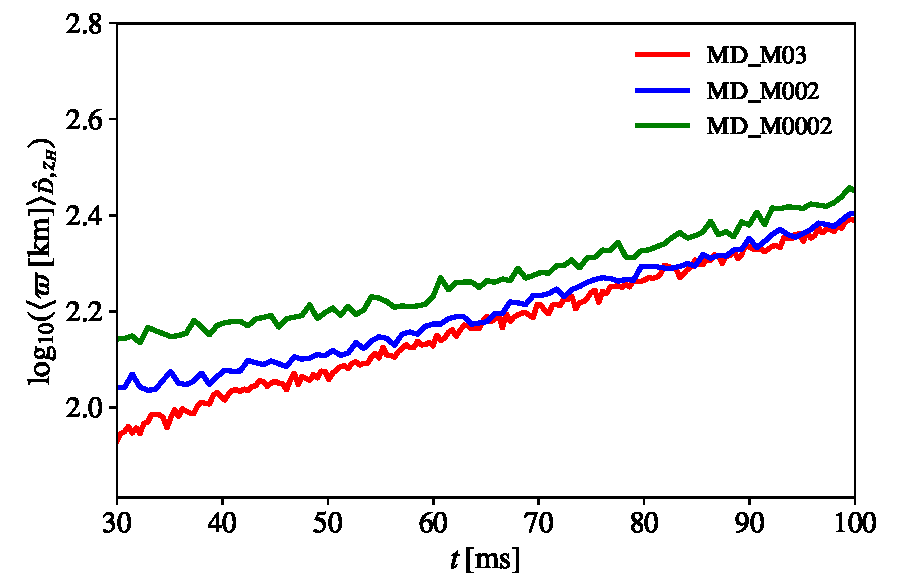
\includegraphics[width=\columnwidth]{figures/kilonova/mean_radius_multi_densav_log.pdf}
 \caption{Top: Black hole accretion rates as a function of time for the three simulation runs in this work. Bottom: Density-averaged cylindrical radius of matter as a function of time, indicating viscous spreading over time. \label{fig:mdot-t}}
%\vspace{5mm}
\end{figure}

\begin{figure}[t]
  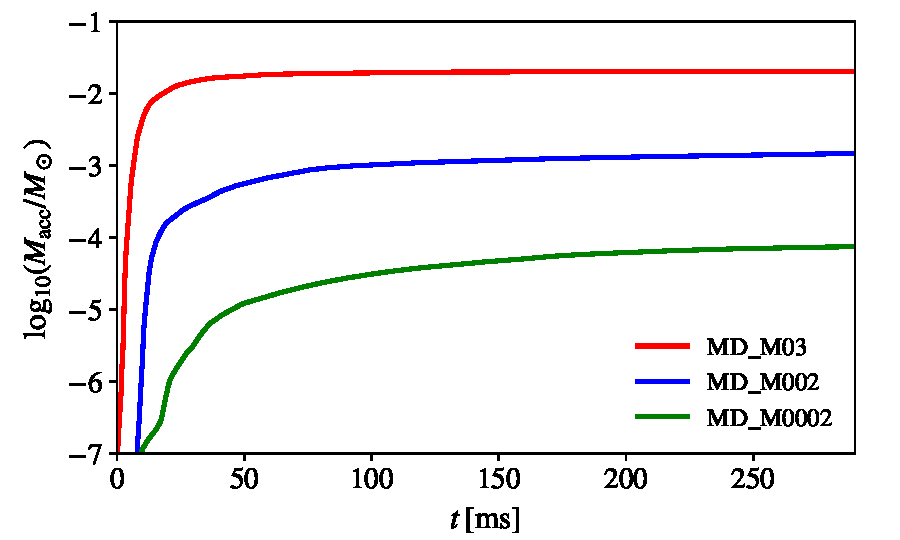
\includegraphics[width=\columnwidth]{figures/kilonova/Macc_multidets_sims.pdf}
 \caption{Top: Black hole accretion rate as a function of time for the three simulation runs in this work. As a result of viscous spreading, the total cumulative accreted mass essentially converges over the duration of the simulation runs, and all remaining material will be eventually unbound from the system. \label{fig:macc-t}}
%\vspace{5mm}
\end{figure}

Magnetic turbulence in the disks generated by the MRI drives accretion onto the black hole at the center, and outward transport of angular momentum in the disks. Figure \ref{fig:mdot-t} shows the evolution of accretion rates $\dot M$ with time for all three simulations. The accretion rates for models \texttt{MD\_M03}, \texttt{MD\_M002}, and \texttt{MD\_M0002}, time-averaged over a 10\,ms window around $t=30$\,ms are $2.6_{-0.7}^{+1.4}\times 10^{-1}~M_\odot s^{-1}$, 
$1.14_{-0.4}^{+0.4}\times 10^{-2}~M_\odot s^{-1}$, and $3.79_{-1.7}^{+2.5}\times 10^{-4}~M_\odot s^{-1}$ respectively; the accretion rate changes by a similar order of magnitude as the disk masses among the three simulation runs, which is expected from one-dimensional disk models.

From one-dimensional disk models (see Appendix \ref{app:ignition_threshold}, Eq.~\eqref{eq:Mdot_1D_2}),
\begin{equation}
    \dot{M} \propto \alpha_{\rm vis} \bar{\rho}_{\rm d} M_{\rm BH}^{1/2} \left(\frac{z_H}{\varpi}\right)^3, \label{eq:Mdot}
\end{equation}
where $\bar{\rho}_{\rm d}$ is the disk density. We compute a representative value for $\bar{\rho}_{\rm d}$ in the inner accretion disk by calculating a three-dimensional spatial average of the disk following Eq.~\eqref{eq:rest_mass_dens_scaleht}, time-averaged over a 10\,ms window around $t=30$\,ms (see Tab.~\ref{tab:torusenergytab}). We note that the quantities, self-consistently set by MHD turbulence in our simulations, roughly satisfy relation \eqref{eq:Mdot}, within the uncertainties in extracting these numbers given the 3D turbulent evolution of the disks.

The bottom panel of Fig.~\ref{fig:mdot-t} shows the early evolution of the density-averaged cylindrical radius of matter $\langle \varpi \rangle_{{\rm azim}, z_H}$ in the simulations, integrated up to the local density scale height. This parameter is roughly representative of viscous radial spreading of the disks. The early evolution shown in Fig.~\ref{fig:mdot-t} is indeed indicative of viscous spreading of our disks.

As measured by the mass flux through a spherical coordinate detector surface placed at a radius of 12~km, the percent initial disk mass accreted by the black hole is $\approx$ 47\%, $\approx$ 60\%, and $\approx$ 31\% for \texttt{MD\_M03}, \texttt{MD\_M002}, and \texttt{MD\_M0002} respectively, by the end of the simulations. Figure \ref{fig:macc-t} shows the evolution of the accreted mass by the black hole over the duration of the simulations. Most of the accretion completes within the first $\sim$ 50-100~ms, after which the accretion rate starts to drop rapidly, with a comparatively negligible amount of mass projected to be accreted onto the black hole past the end of the simulation. We ascribe this effect to viscous spreading of the disks, which forces the disk material remaining at the end of the simulations to eventually be unbound from the system in the form of winds. Properties of ejecta are discussed in Sec.~\ref{sec:ejecta}.

%$z_H$ of the disk, defined as (cf. Equations 62 and 63 of \citet{Siegel:2017jug})
%\begin{equation}
%    z_H (\varpi) = \frac{\int \int_0^{2\pi} |z|\hat D \varpi d\phi dz}{\int \int_0^{2\pi} \hat D \varpi d\phi dz},
%\end{equation}
%where $\hat D = \sqrt{\gamma} \rho W$ is the conserved rest mass density, with $\gamma$ being the determinant of the spatial metric
%$\gamma_{ij}$ and $W$ the Lorentz factor. In this way, we explicitly exclude the disk corona and winds from the integration.


\subsubsection{Neutrino emission}
\label{sec:neutrino_emission}

\begin{figure*}[t]
  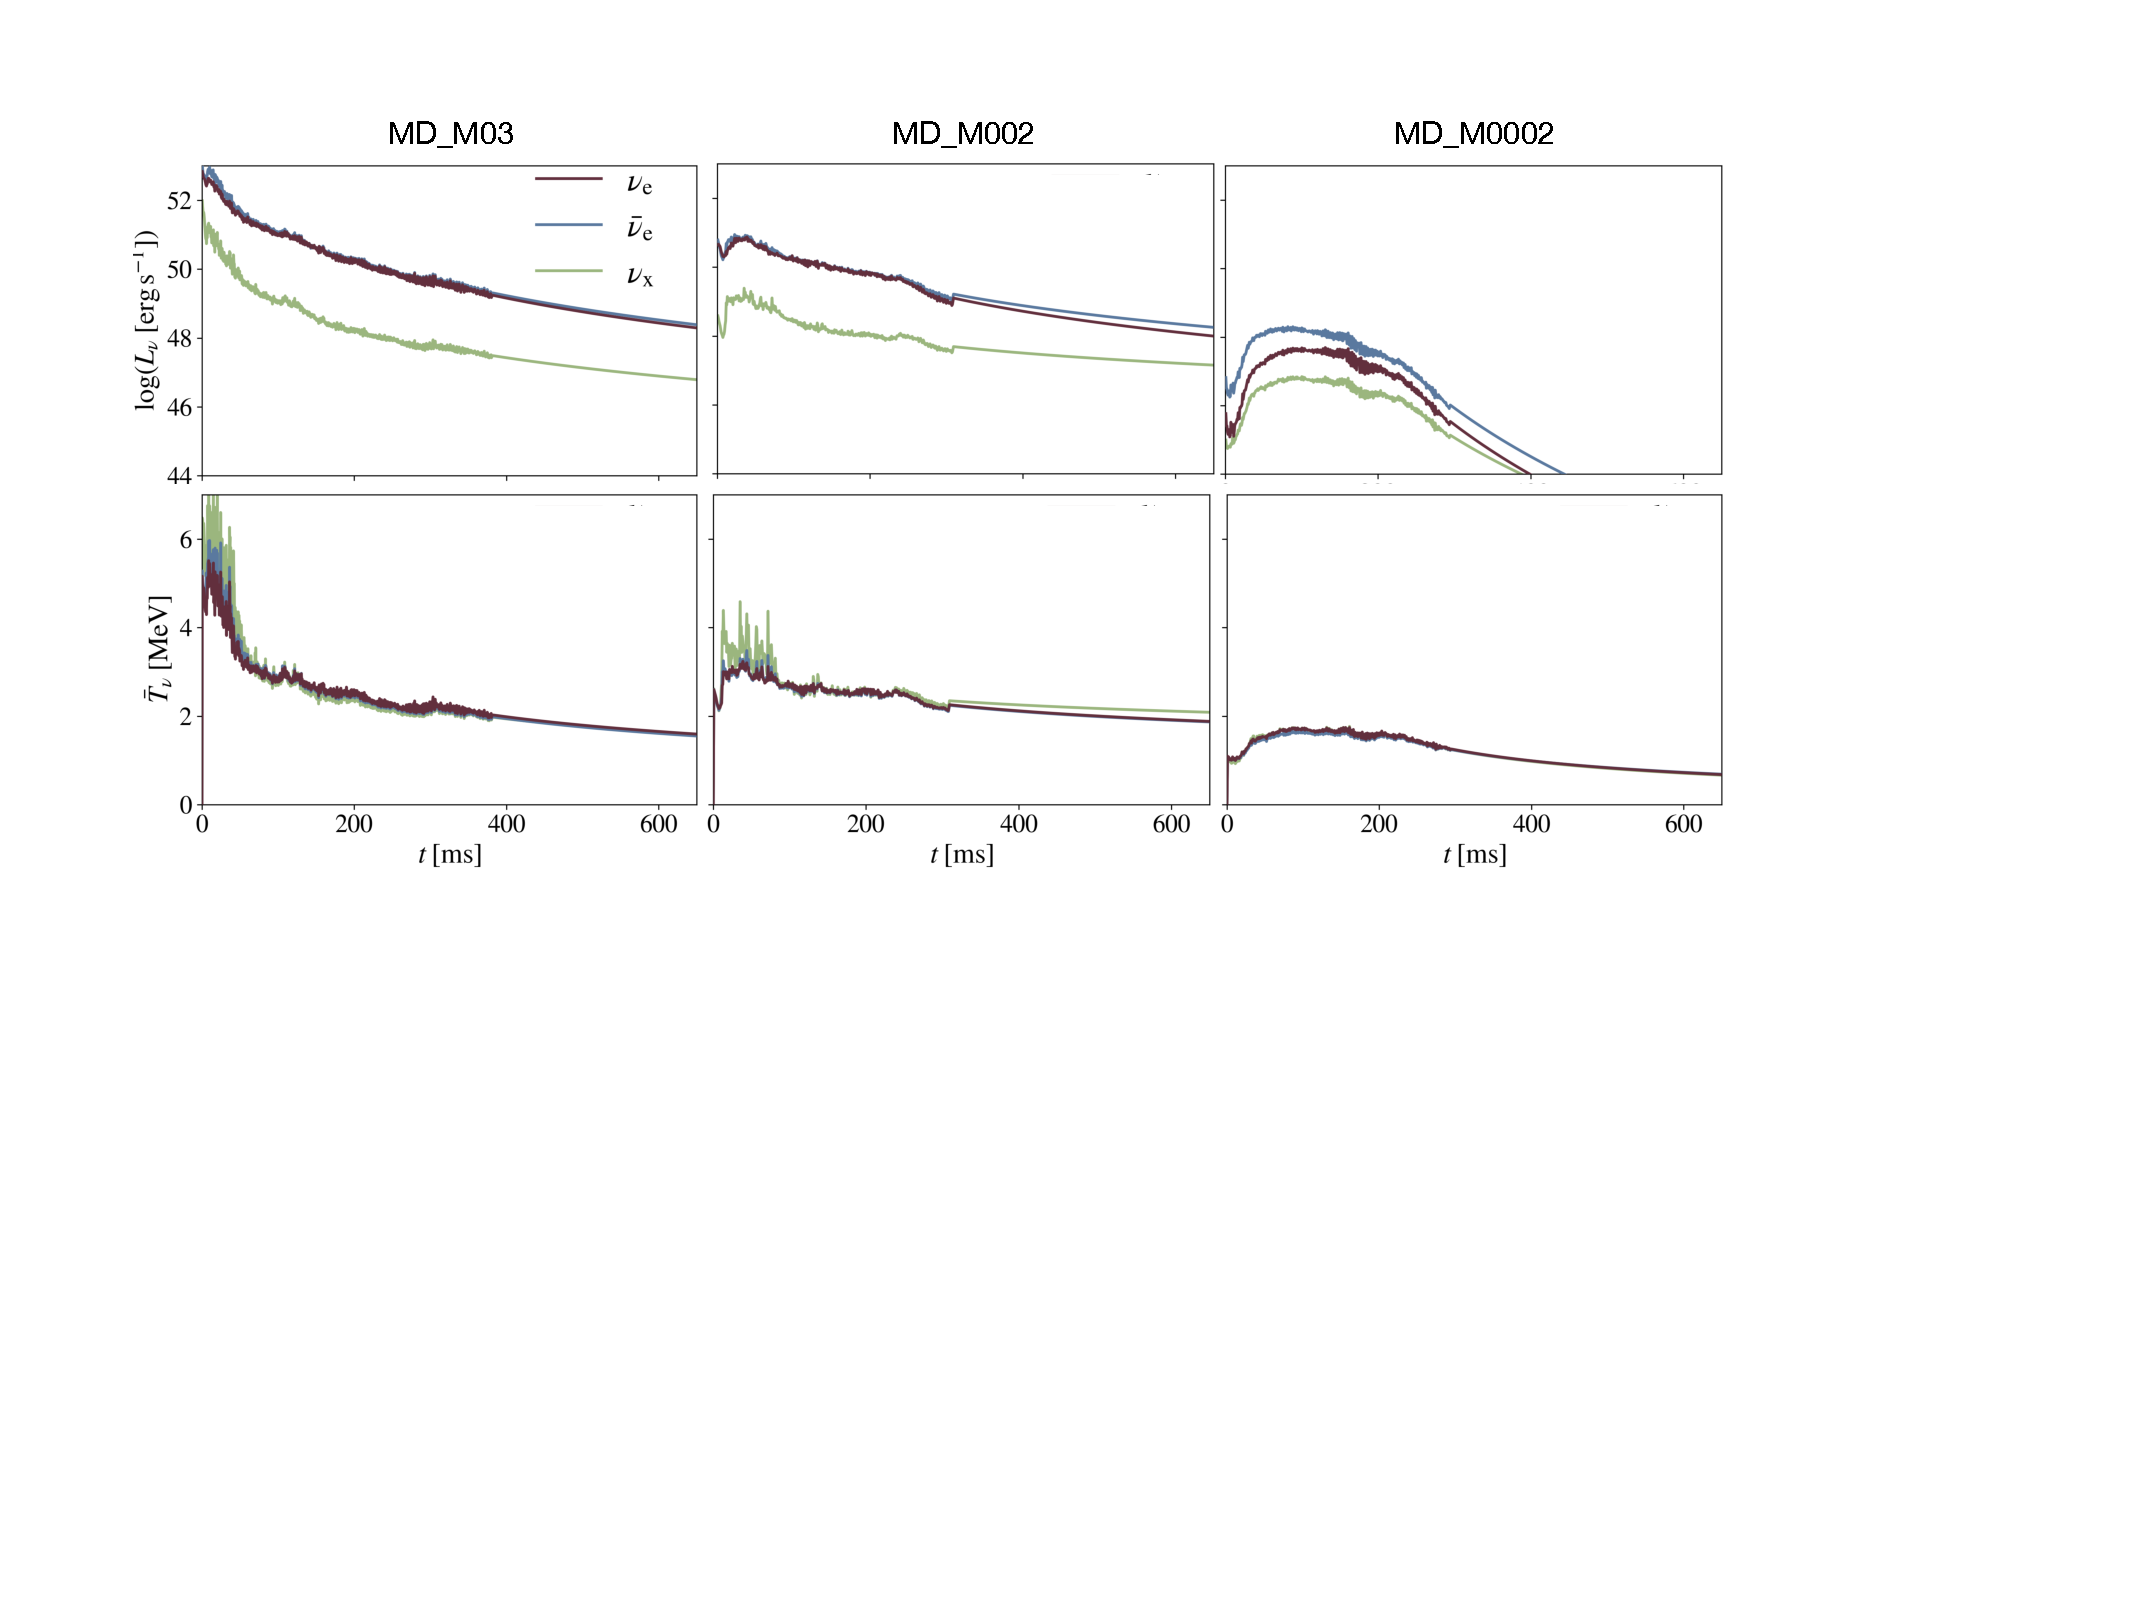
\includegraphics[width=\textwidth]{figures/kilonova/Lum_temp_nu_plots.pdf}
 \caption{Characteristics of neutrino emission from the disk models in this work. The top panels show total neutrino luminosity and the bottom panels show mean neutrino emission temperature. The simulations end at $t \sim\!290$~ms after which the quantities are extrapolated by power law fits to late times.\label{fig:Lum_temp_nu}}
%\vspace{5mm}
\end{figure*}

\begin{figure}[t]
  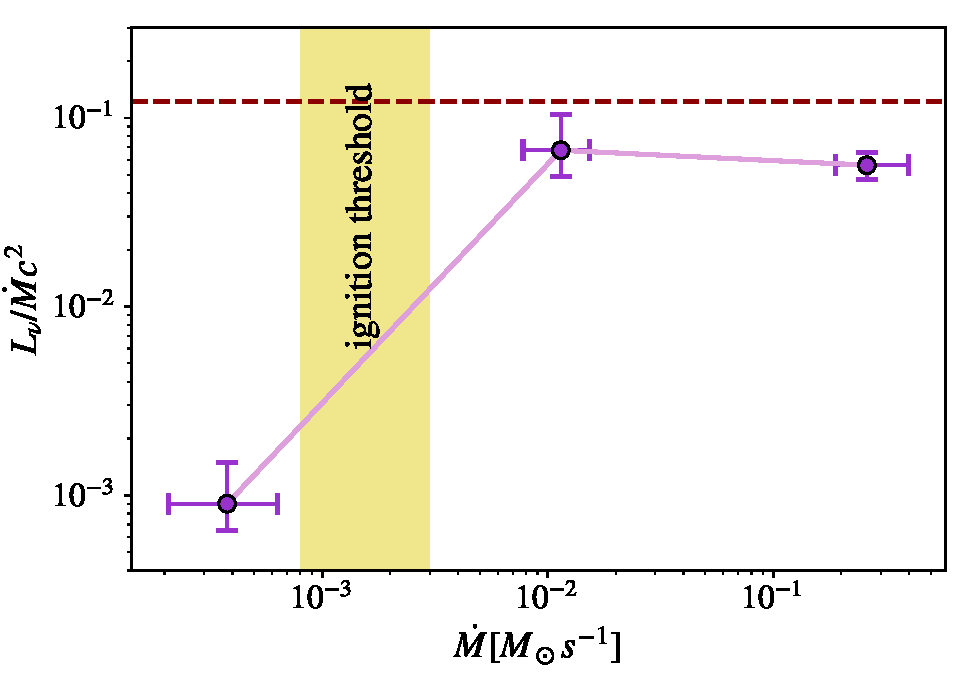
\includegraphics[width=\columnwidth]{figures/kilonova/lum_mdot.pdf}
 \caption{Radiative efficiency as a function of accretion rate for accretion on to a black hole with mass $3~M_\odot$ and dimensionless spin 0.8, as derived from the simulations in this work. The efficiency rises with increasing $\dot M$, reaches a maximum just above the ignition threshold $\dot{M}_{\rm ign}\sim 1\times 10^{-3}\,M_\odot\,{\rm s}^{-1}$ (cf.~Eq.~\eqref{eq:Mdot_ign_merger}), then decreases with increasing $\dot M$. The black dashed line shows the maximum radiative efficiency possible in such a system (see the text for details).\label{fig:lum-mdot}}
%\vspace{5mm}
\end{figure}

Figure \ref{fig:Lum_temp_nu} shows properties of neutrino radiation from the disks for all neutrino species $\nu_i \in {\nu_{e}, \bar \nu_{e}, \nu_{x}}$, where $\nu_{x}$ represents all heavier neutrino species collectively. As in Ref. \cite{Siegel:2017jug}, we define the total neutrino luminosity $L_\nu$ of a given species and the corresponding mean neutrino emission temperature $\bar T_\nu$ as
\begin{equation}
    L_{\nu_i} = \int \alpha W Q_{\nu_i}^{\rm eff} \alpha\sqrt{\gamma}d^{3}x,
\end{equation}
and
\begin{equation}
    \bar T_{\nu_i} = \frac{\int TQ_{\nu_i}^{\rm eff}W\alpha\sqrt{\gamma}d^{3}x}{\int Q_{\nu_i}^{\rm eff}W\alpha\sqrt{\gamma}d^{3}x},
\end{equation}
respectively. Here, $Q_{\nu_i}^{\rm eff}$ is the effective neutrino emissivity, $W$ is the Lorentz factor, and $\alpha$ is the lapse function. We fit power laws to the late time simulation data to extrapolate these quantities beyond the time range modeled in the simulations. Figure \ref{fig:Lum_temp_nu} shows that the electron and anti-electron neutrino luminosities are at least an order of magnitude higher than the heavier neutrino luminosities. Emission channels for the heavier species are relatively suppressed at the comparatively low densities and temperatures of such accretion disks. Luminosities are typically maximal initially when the turbulent state has been established and the disks are still compact and in their high-density and high-temperature regime. Table \ref{tab:torusenergytab} reports the total $L_\nu$-value for $\nu_e$ and $\bar{\nu}_e$ for each simulation run, extracted as an average over a $10$\,ms time-window around the peak luminosities of the respective runs. These range between $\approx\!1\times 10^{52}$\,erg\,s$^{-1}$ (\texttt{MD\_M03}) and $\approx\!1\times 10^{48}$\,erg\,s$^{-1}$ (\texttt{MD\_M0002}). %Table \ref{tab:torusenergytab} reports the initial total $L_\nu$-value for $\nu_e$ and $\bar{\nu}_e$ for each simulation run, extracted as an average over a $10$\,ms time-window centered at the simulation time $t = 30$\,ms, which range between $\approx\!1\times 10^{52}$\,erg\,s$^{-1}$ (\texttt{MD\_M03}) and $\approx\!1\times 10^{48}$\,erg\,s$^{-1}$ (\texttt{MD\_M0002}). 
At later simulation times, as the accretion disks spread radially and become less compact, luminosities start to quickly fade over the timescales of the simulations. This indicates the neutrino self-irradiation of outflows in the context of r-process nucleosynthesis (see Sec.~\ref{sec:nucleosynthesis}) is likely only important initially, and much less so for the less luminous disks \texttt{MD\_M002} and \texttt{MD\_M0002}.
%for \texttt{MD\_M03} and \texttt{MD\_M002}, irradiation by neutrinos in the early part of the disk evolution can have an appreciable effect on the outflows and $r$-process nucleosynthesis. For \texttt{MD\_M0002}, neutrino irradiation is not strong enough to modify the composition of outflows.



The qualitatively different behavior of our disk models in terms of weak interactions is captured by the differences in radiative efficiency $L_\nu/\dot M c^2$ among the simulations. Figure \ref{fig:lum-mdot} shows the variation of the radiative efficiency of the disks as a function of their accretion rate $\dot M$. The ratio $L_\nu/\dot M c^2$ represents the amount of accreted rest-mass energy that is turned into radiation per unit time. In order to assess radiative efficiency, for each simulation, we extract $L_\nu$ and $\dot M$ as mean values over the time range $t = 25-35$~ms. Fig.~\ref{fig:lum-mdot} shows the resulting efficiencies of $5.61^{+0.9}_{-0.9}\times 10^{-2}$, $6.73^{+3.7}_{-1.8}\times 10^{-2}$, and $9.01^{+6.0}_{-2.5}\times 10^{-4}$ for \texttt{MD\_M03}, \texttt{MD\_M002}, and \texttt{MD\_M0002}, respectively, compared to the maximum possible radiative efficiency. The latter is a fundamental limit on the amount of energy that can be extracted from a black hole accretion flow, determined by the available binding energy \cite{thorne_disk-accretion_1974}, 
\begin{equation}
    [L_\nu/\dot M c^2]_{\rm max} = 1 - E_{\rm ms},
\end{equation}
where
\begin{equation}
    E_{\rm ms} = \frac{1 - 2M_{\rm BH}}{3r_{\rm ms}}
\end{equation}
is the specific energy at the marginally stable circular orbit of a Kerr black hole \cite{bardeen_rotating_1972}
\begin{equation}
    r_{\rm ms} = M_{\rm BH}\{3 + Z_2 \mp [(3 - Z_1)(3 + Z_1 + 2Z_2)]^{1/2}\},
\end{equation}
with
\begin{eqnarray}
    Z_1 &=& 1 + (1 - \chi_{\rm BH}^2/M_{\rm BH}^2)^{1/3}[(1 + \chi_{\rm BH}/M_{\rm BH})^{1/3} \nonumber\\
    &&+ (1 - \chi_{\rm BH}/M_{\rm BH})^{1/3}], \\
    Z_2 &=& (3\chi_{\rm BH}^2/M_{\rm BH}^2 + Z_1^2)^{1/2}.
\end{eqnarray}

The efficiency in realistic scenarios, as also seen from the simulation data in Fig.~\ref{fig:lum-mdot}, is smaller than the maximum theoretical value, as a fraction of the binding energy is stored in the disk and radially advected into the black hole in the form of heat. The amount of heat radiated away thus depends on the efficiency of radiative processes with respect to radial advection of energy (cf.~Appendix \ref{app:ignition_threshold}). At low $\dot M$ values, the low midplane densities and temperatures in the inner disk suppress neutrino emission, resulting in a low radiative efficiency. As $\dot M$ increases, higher midplane densities and temperatures enhance neutrino emission, causing the radiative efficiency to rise and to reach a maximum just above the ignition threshold (Sec.~\ref{sec:intro_ignition_threshold} and Appendix~\ref{app:ignition_threshold}). As $\dot M$ increases further, neutrino cooling continues to become more effective, but at the same time the accretion timescale eventually becomes shorter than the neutrino cooling timescale: the very high $\dot M$ values lead to high midplane densities (cf.~Eq.~\eqref{eq:Mdot}) and thus to an increase in the optical depth in the midplane, eventually trapping neutrinos and reducing the cooling volume, enhancing radial advection of energy and decreasing the radiative efficiency. 

This behavior is evident from Fig~\ref{fig:lum-mdot}, which shows a stark rise in radiative efficiency between the runs \texttt{MD\_M0002} and \texttt{MD\_M002} around an ignition threshold of $\dot{M}_{\rm ign}\sim 1\times 10^{-3}\,M_\odot\,{\rm s}^{-1}$ as predicted by Eq.~\eqref{eq:Mdot_ign_merger}. For even  more massive accretion disks, a decline in the radiative efficiency would be expected (see also \cite{chen_neutrino-cooled_2007}), but such disks are beyond the scope of the present study. We note that our results are qualitatively consistent with previous studies from one-dimensional disk models \cite{chen_neutrino-cooled_2007}.



%\begin{figure}[t]
%\includegraphics[width=\columnwidth]{mean_radius_plot.pdf}
% \caption{\label{fig:mean-radius}}
%\vspace{5mm}
%\end{figure}


\subsubsection{Ejecta}
\label{sec:ejecta}

\begin{figure*}[t]
  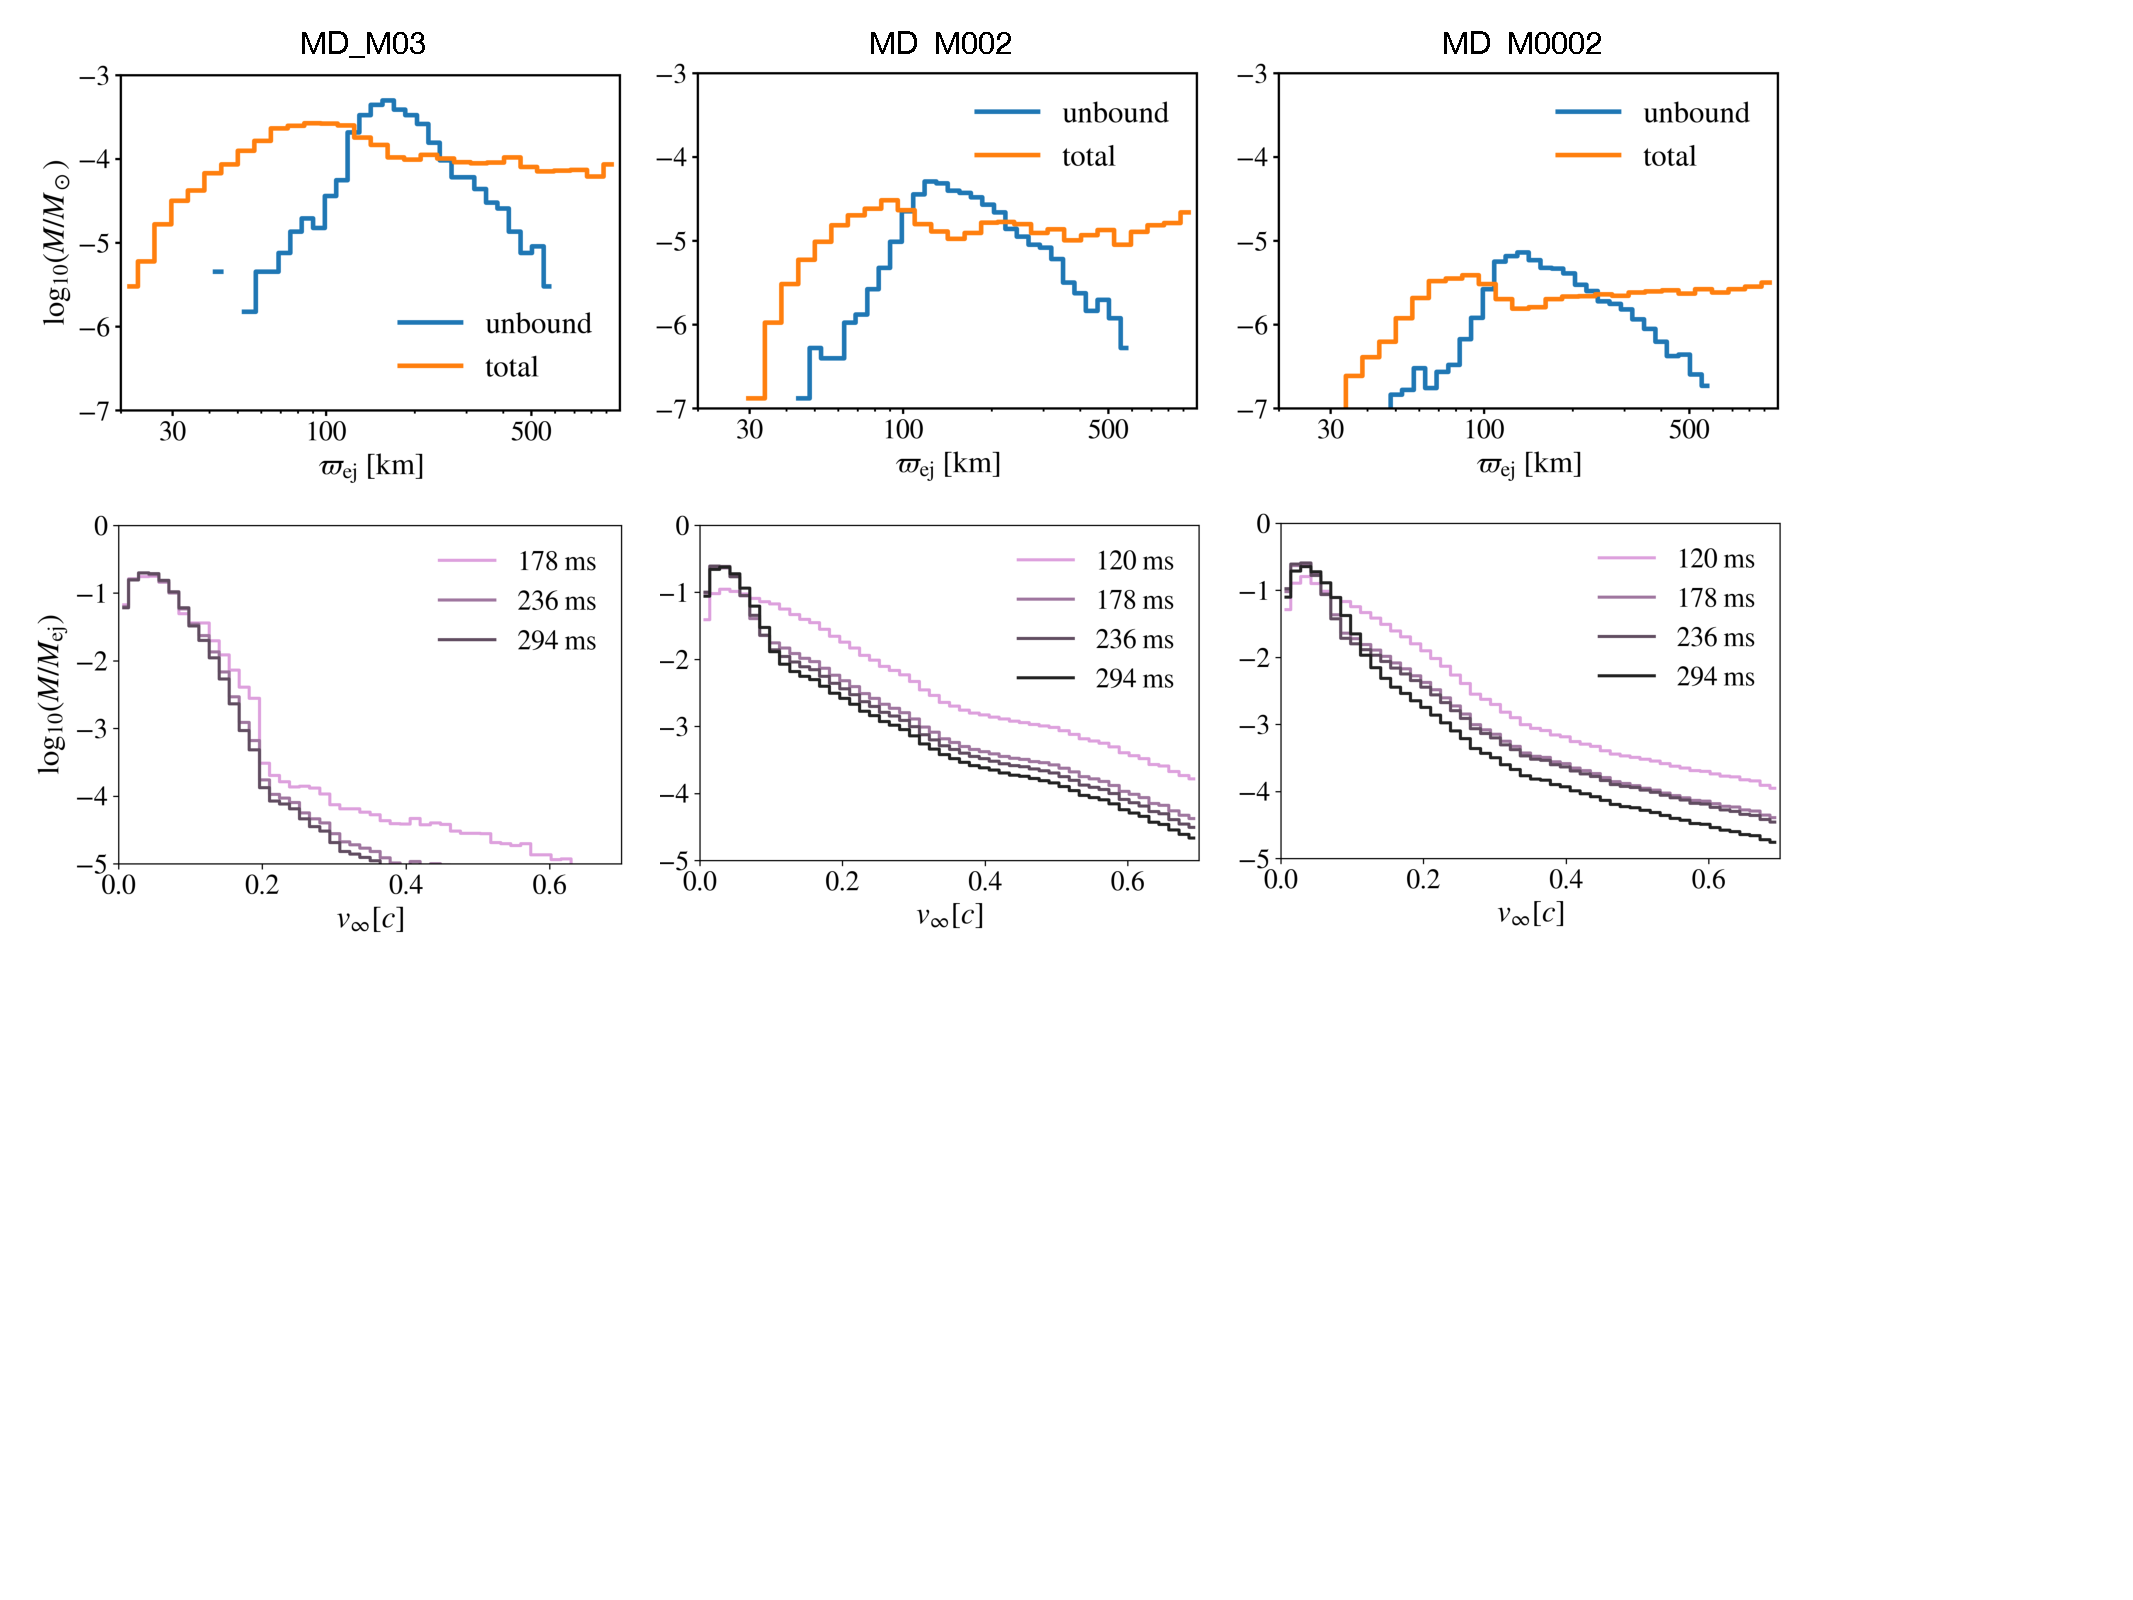
\includegraphics[width=\textwidth]{figures/kilonova/mass_vs_velocity_tracers_n_outflow.pdf}
 \caption{Outflow properties of the three accretion disks simulated in this work. Top: Mass distribution of unbound and total outflows as recorded by tracer particles in terms of their cylindrical radius $\varpi_{\rm ej}$ at which they get ejected from the disk corona. Bottom: Mass distributions of unbound outflows (normalized by the total disk outflow) in terms of their asymptotic escape velocities $v_\infty$. These measurements are performed by recording the properties of outflowing material through a spherical coordinate detector surface placed at a radius of 1034~km from the black hole.\label{fig:outflows}}
\end{figure*}

Outflows from the disks originate in high specific entropy (`hot') disk coronae as a result of an imbalance between heating and cooling at high latitudes. Viscous heating as well as dissipation of magnetic energy far from the midplane is not offset by neutrino cooling, which becomes energetically subdominant at the comparatively low densities off the midplane. The precise amount of material unbound from the disk depends on the details of the self-consistent heating-cooling imbalance generated by MHD turbulence. We refer to Ref. \cite{Siegel:2017jug} for a detailed discussion on the emergence of these outflows in the presence of MHD turbulence.

%Accretion of material onto the black hole causes an increase of density and temperature in the disk midplane. As neutrino emission follows density, these regions effectively participate in neutrino emission, which provide a cooling mechanism to balance the MHD heating. The rate of neutrino emission depends on the rate of accretion onto the black, as illustrated in Section \ref{sec:disk_composition}. Away from the disk midplane, the disk density drops rapidly, which causes a drop in the rate of neutrino emission. This creates an imbalance between the rate of heating from MHD turbulence and the rate of cooling from neutrino emission, resulting in regions of high entropy, which we refer to as the ``corona'', above and below the disk midplane. The low density corona regions then gives rise to strong outflows. 

We track properties of these outflows using $10^4$ tracer particles of equal mass, placed throughout the disk initially, with probability density proportional to the conserved rest mass density $\hat D = \sqrt \gamma \rho W$. The top panels of Fig.~\ref{fig:outflows} show the mass distribution of total and unbound disk outflow (ejecta) as recorded by the tracer particles in terms of the cylindrical radius at which the tracer particles are ejected from the disk corona, the latter begin defined as the cylindrical radius after which their radial coordinate position only increases with time. We define unbound material as having reached a coordinate radius of $10^3$\,km and additionally having positive specific energy at infinity, $-hu_0 > 0$, where $h$ denotes the specific enthalpy and $u_0$ is the 0-component of the fluid four-velocity. For all simulations, we find that the total outflow material is almost evenly distributed over a broad  range of radii, whereas the majority of the ejecta mass originates from the inner accretion disk ($\varpi\lesssim100-250$~km), where most of the binding energy is released through viscous heating. The total amount of material ejected by the disks are $3.179\times 10^{-3}~M_\odot (\approx 10\%$ of the initial disk mass) for \texttt{MD\_M03}, $4.03\times 10^{-4}~M_\odot (\approx 20\%$ of the initial disk mass) for \texttt{MD\_M002}, and $6.046\times 10^{-5}~M_\odot (\approx 30\%$ of the initial disk mass) for \texttt{MD\_M0002} by the end of the simulations. The disks still generate steady winds at the end of our simulations, which indicates that the remaining disks would continue evaporating themselves if the simulations were evolved over longer timescales. Given that the total cumulative accreted masses have already converged over the duration of the simulation runs (cf.~Sec.~\ref{sec:accretion}), we predict that the remaining disk will generate outflow material corresponding to $\approx\! 37\%$ of the initial disk mass for \texttt{MD\_M03}, $\approx\! 18\%$ of the initial disk mass for \texttt{MD\_M002}, and $\approx\! 38\%$ of the initial disk mass for \texttt{MD\_M0002}. This material will be ejected over longer timescales by a combination of the MHD-driven outflows as discussed here and viscous spreading of the disk over several viscous timescales (see \cite{fernandez_long-term_2019} for a discussion of late-time viscous outflows).

The bottom panels of Figure \ref{fig:outflows} show the distribution of asymptotic ejecta velocity for the three simulation runs as measured from the mass flux through spherical coordinate detector surfaces placed at a radius of 1034\,km. The asymptotic velocities $v_\infty$ are computed from the asymptotic Lorentz factor $W_\infty = -hu_0$ as measured by the detector sphere. In all three simulations, we find the emergence of a high-velocity tail, with the bulk ejecta residing around $v_\infty\approx 0.1c$. This velocity scale is naturally explained as a combination of moderate outflow velocities from the hot corona of typically $(0.03-0.1)c$ together with the energy released by recombination of individual nucleons into $\alpha$-particles ($\approx\!7$\,MeV per baryon per $\alpha$-particle formed). Our velocity distributions are qualitatively similar to Refs. \cite{Fernandez:2018kax} and \cite{Christie:2019lim}, albeit their GRMHD run---similar to our \texttt{MD\_M03} case---shows more outflow mass at higher velocities; this has been commented on in Ref. \cite{Fernandez:2018kax} and can be attributed in part to their initial magnetic field configuration, which is optimized for fast magnetically-dominated outflows. The high-velocity tail for the low-$\dot{M}$ disks \texttt{MD\_M002} and \texttt{MD\_M0002} are more pronounced, which may be ascribed to more violent viscous heating as neutrino cooling becomes less important at low accretion rates.




\subsection{Weak interactions and disk composition}
\label{sec:disk_composition}

\begin{figure*}[t]
\centering
  \includegraphics[width=16cm]{figures/kilonova/snapshot_43_130_250_Ye_logetae_xy_MD_M03_M002_M0002.pdf}
 \caption{Snapshots of the electron fraction $Y_e$ and electron degeneracy $\eta=\mu_e/k_{\rm B}T$ over time for the three simulation runs performed here. Plotted are slices of these quantities in the disk midplane ($x$-$y$ plane) at times $t = 42.8$~ms, $t = 130$~ms, and $t = 250$~ms. Above the ignition threshold for weak interactions (Eq.~\eqref{eq:Mdot_ign_merger}), the high accretion rates of runs \texttt{MD\_M03} and \texttt{MD\_M002} cause the inner disk to remain strongly neutron-rich over time, whereas below the ignition threshold the low accretion rate of run \texttt{MD\_M0002} leads to accelerated protonization in the inner part. \label{fig:panels_Ye_eta}}
\vspace{5mm}
\end{figure*}


\begin{figure*}[t]
\centering
  \includegraphics[width=16cm]{figures/kilonova/snapshot_43_130_250_R_eff_nua_nue-entropy_xy_M03_M002_M0002.pdf}
 \caption{Evolution of the ratio of anti-electron to electron neutrino number emission rates $R_{\bar \nu_{\rm e}}^{\rm eff}/R_{\nu_{\rm e}}^{\rm eff}$ and specific entropy $s$ for the three simulation runs performed here. Plotted are snapshots of these quantities in the disk midplane ($x$-$y$ plane) at times $t = 42.8$~ms, $t = 130$~ms, and $t = 250$~ms.\label{fig:panels_R_eff_entropy}}
\vspace{5mm}
\end{figure*}

Accretion disks below and above the ignition threshold for weak interactions give rise to qualitatively different evolution of its composition as we shall illustrate in this section. Discussing weak interactions in the disk in more detail also benefits the interpretation of the behavior of some global disk quantities (Sec.~\ref{sec:global_properties}) as well as of nucleosynthesis in disk outflows (Sec.~\ref{sec:nucleosynthesis}).

Figures \ref{fig:panels_Ye_eta} and \ref{fig:panels_R_eff_entropy} show various quantities pertaining to the evolution of disk composition, including snapshots of the electron fraction, electron degeneracy $\eta=\mu_e/k_{\rm B}T$, where $\mu_e$ is the electron chemical potential, the ratio of $\bar{\nu}_e$ to $\nu_e$ number emission rates ($R_{\bar \nu_{\rm e}}^{\rm eff}/R_{\nu_{\rm e}}^{\rm eff}$), and specific entropy $s$ over the course of the three simulation runs.

Neglecting absorption of neutrinos, appropriate for the disk midplane, the weak interactions controlling disk composition are the charged-current $\beta$-processes,
\begin{eqnarray}\label{eq:proton_capture}
      e^- + p &\rightarrow& n + \nu_{\rm e}, \label{eq:proton_capture} \\
      e^+ + n &\rightarrow& p + \bar \nu_{\rm e}. \label{eq:neuton_capture}
\end{eqnarray}
Starting off from neutron-rich initial conditions $Y_e\approx 0.1$ (cf.~Sec.~\ref{sec:methods}), one expects the disks to protonize over time due to Eq.~\eqref{eq:neuton_capture} dominating. This is evident from $R_{\bar \nu_{\rm e}}^{\rm eff}/R_{\nu_{\rm e}}^{\rm eff}>0$ and the gradual increase of $Y_e$ over time of in the outer parts of the accretion disks in Figs.~\ref{fig:panels_R_eff_entropy} and \ref{fig:panels_Ye_eta}. However, less massive disks with lower $\dot{M}$ such as \texttt{MD\_M002} and \texttt{MD\_M0002} take longer times compared to \texttt{MD\_M03} to raise their electron fraction from its initial value; this can be understood from an analysis of the disk protonization timescale.

From the equations of lepton number and baryon number conservation, we
compute
\begin{equation}
  R = \nabla_\mu(n_e u^\mu) = \nabla_\mu(n_{\rm b} u^\mu Y_e) = n_{\rm b} u^\mu
  \nabla_\mu Y_e,
\end{equation}
and thus
\begin{equation}
  u^\mu \nabla_\mu Y_e = R \frac{m_{\rm b}}{\rho}, \label{eq:Y_e_cons}
\end{equation}
where $u^\mu$ is the four-velocity of the fluid and $R$ denotes a source term to account for the change in lepton number due to weak interactions. Equation \eqref{eq:Y_e_cons} shows that along a fluid trajectory, i.e., in the comoving frame of the fluid, the electron fraction changes by a rate of $R m_{\rm b}/ \rho$. We can therefore define the characteristic timescale for the composition of matter to change by $t_{Y_e} \equiv Y_e\rho / (R m_\mathrm{b})$. Neglecting neutrino absorption, appropriate for the disk midplane, one has
\begin{equation}
  t_{Y_e} = \frac{Y_e}{R_{\bar{\nu_e}}^\mathrm{eff} -
    R_{\nu_e}^\mathrm{eff}}\frac{\rho}{m_{\rm b}}. \label{eq:t_Ye}
\end{equation}
Ignoring final state blocking in the neutrino phase space, the effective emission rates scale as \cite{tubbs_neutrino_1975,Bruenn:1985en} $R_{\bar{\nu}_e,\nu_e}^\mathrm{eff} \propto \rho T^5 \propto \dot{M}^{9/4}$, where we have used the approximate expression Eq.~\eqref{eq:T_1D} for the midplane temperature in the second step. Furthermore, since $\dot{M}\propto \rho$ (cf.~Eq.~\eqref{eq:Mdot_1D_2}), we deduce that, approximately,
\begin{equation}
  t_{Y_e} \propto \dot{M}^{-5/4},  \label{eq:t_Ye_scale_Mdot}
\end{equation}
which explains the decrease in protonization timescale with increasing accretion rate seen in the outer accretion disks in Figs.~\ref{fig:panels_Ye_eta} and \ref{fig:panels_R_eff_entropy}.

The inner accretion disk shows qualitatively different behavior depending on whether the accretion disk resides in a state above or below the ignition threshold (Eq.~\eqref{eq:Mdot_ign_merger}, Sec.~\ref{sec:neutrino_emission}). We find that above the ignition threshold, the disk midplane density $\rho\propto \dot{M}$ (cf.~Eq.~\eqref{eq:Mdot_1D_2}) is sufficiently large that electrons become degenerate, as shown in Fig.~\ref{fig:panels_Ye_eta}. This, in turn, suppresses positron creation via $\gamma\rightarrow e^+ + e^-$ and thus Eq.~\eqref{eq:neuton_capture} relative to \eqref{eq:proton_capture}, and hence leads to slight neutronization even in very neutron-rich initial conditions (see \texttt{MD\_M03} in Fig.~\ref{fig:panels_R_eff_entropy}). This neutronization mechanism is also the reason why collapsar accretion disks starting with much higher $Y_e$ were found to be able to generate neutron-rich outflows and synthesize r-process elements \cite{siegel_collapsars_2019}. However, the inner parts of the accretion disks cannot become arbitrarily degenerate and neutron rich, thanks to a self-regulation mechanism discussed in Ref. \cite{Siegel:2017jug} and previously pointed out by Ref. \cite{chen_neutrino-cooled_2007}. As shown in Fig.~\ref{fig:panels_Ye_eta}, disk self-regulation leads to a heating-cooling balance that results in moderate electron degeneracy $\eta\sim 1$ and corresponding neutron richness of $Y_e\approx 0.1$. At lower $\dot{M}$, close to the ignition threshold, degeneracy and self-regulation become somewhat weaker and less pronounced; however, \texttt{MD\_M002} still qualitatively shows the same behavior as \texttt{MD\_M03}. We also note that as a result of viscous spreading, the disk density decreases over time, which may suppress degeneracy eventually late in the disk's evolution. The onset of a decrease in degeneracy is noticeable from the snapshots in Fig.~\ref{fig:panels_Ye_eta}. However, by the time massive disks such as \texttt{MD\_M03} reach this break-down of degeneracy, most disk material has been evaporated and the change in disk composition has little effect on the overall composition of ejecta. While the disk is in such a self-regulated, moderately degenerate phase, the inner part of the accretion disk feeds highly neutron-rich material into the outflows.

Below the ignition threshold, we find an inverted scenario in terms of midplane composition within the inner parts of the accretion disk. The timescale for protonization in the innermost part of the accretion disk is significantly smaller than in the outer parts, resulting in a high-$Y_e$ surrounding of the black hole already at $t\sim100$\,ms (cf.~\texttt{MD\_M0002} in Fig.~\ref{fig:panels_Ye_eta}). We attribute this to excess viscous heating in the absence of energetically significant neutrino cooling. The resulting high-entropy environment (cf.~Fig.~\ref{fig:panels_R_eff_entropy}) leads to a prolific generation of positrons via pair production, $\gamma\rightarrow e^+ + e^-$, and thus decreases the timescale for protonization via Eq.~\eqref{eq:neuton_capture}. This innermost region in \texttt{MD\_M0002} is too small, however, to feed material into the outflows sufficient enough for a pronounced high-$Y_e$ tail of the ejecta (cf.~Sec.~\ref{sec:nucleosynthesis}).


%Figure \ref{fig:panels_Ye_eta} shows the variation of the electron fraction $Y_e$ and the electron degeneracy $\eta$, and \ref{fig:panels_R_eff_entropy} shows the variation of the ratio of neutrino number emission rate to antineutrino number emission rate and entropy over the course of the threes simulations. We find that the overall pattern of variation of disk properties in terms of these parameters are similar for the high disk mass cases \texttt{MD\_M03} and \texttt{MD\_M002}, where weak interactions are important. For the lowest disk mass case \texttt{MD\_M0002}, we see a difference in the disk properties, determined by negligible weak interactions. We notice that for \texttt{MD\_M03} and \texttt{MD\_M002}, the disks have low $Y_{\rm e}$ inside and high $Y_{\rm e}$ outside, whereas for \texttt{MD\_M0002}, the pattern reverses, with the inner disk having high $Y_{\rm e}$ and the outer disk having low $Y_{\rm e}$. The disk physics is controlled by the following processes:
%\begin{enumerate}[i)]
%  \item charged current $\beta$-processes \\
%  \begin{equation}\label{eq:proton_capture}
%      e^- + p \rightarrow n + \nu_{\rm e}
%  \end{equation}
%  \begin{equation}\label{eq:neuton_capture}
%      e^+ + n \rightarrow p + \bar \nu_{\rm e}
%  \end{equation}
%  \item electron-positron pair production
%  \begin{equation}\label{eq:pair_prod}
%      \gamma \rightarrow e^+ + e^-
%  \end{equation}
%\end{enumerate}

%In \texttt{MD\_M03} and \texttt{MD\_M002}, Equation \ref{eq:neuton_capture} is favored in the outer disks, as the disks start neutron rich, causing this region to protonize over time, increasing the ratio of $\bar \nu_{\rm e}$ to $\nu_{\rm e}$ production. The decreasing $\nu_{\rm e}$ production decreases the amount of cooling, causing the entropy to rise over time. $\dot M$ in these simulations is fairly high, leading to high densities in the inner disks. The high density causes $e^-$ degeneracy, and inhibits Equation \ref{eq:pair_prod}. The lack of $e^+$ production suppresses Equation \ref{eq:neuton_capture}, and the disk neutronizes over time.

%For \texttt{MD\_M0002}, $\dot M$ is significantly low, leading to very low density in the inner disk. As $\nu_{\rm e}$ emission tracks density, this leads to the absence of $\nu_{\rm e}$ cooling, and as a result, an increase in entropy. The high entropy causes Equation \ref{eq:pair_prod} to proceed efficiently. The increased amount of $e^+$ produced stimulates Equation \ref{eq:neuton_capture}, protonizing the disk over time. In the outer disk, \ref{eq:neuton_capture} is again is expected to be favored over \ref{eq:proton_capture}, as the disk starts neutron rich. However, there is no pile up of heat in this region, due to which the rates of these reactions are low.

%Although \ref{eq:neuton_capture} is favored over \ref{eq:proton_capture} throughout the simulation, in the inner disk, the sufficient amount of 






\subsection{Nucleosynthesis}
\label{sec:nucleosynthesis}

\begin{figure}[t]
  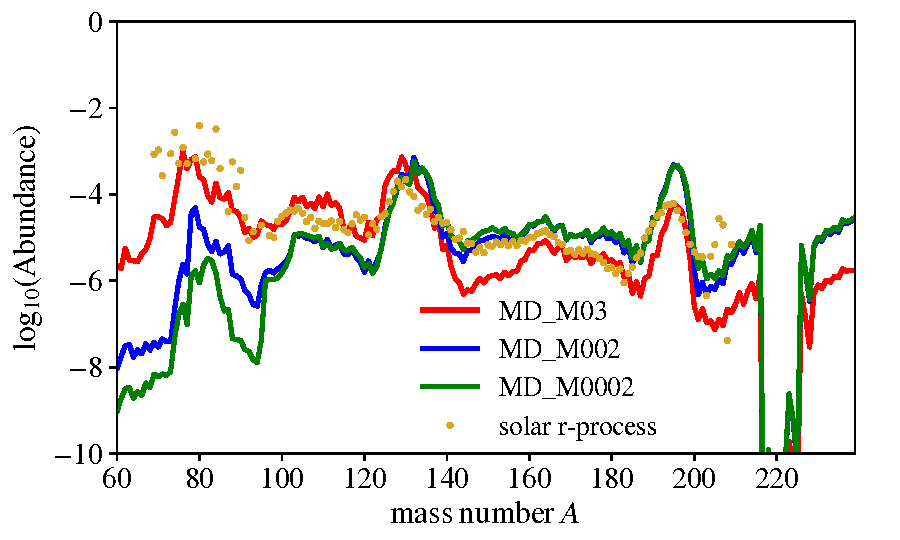
\includegraphics[width=\columnwidth]{figures/kilonova/final_abundances_sims_comparison_MD_M03-MD_M002-MD_M0002.pdf}
 \caption{Final elemental abundances at $10^9$\,s for the accretion disk ejecta of our three simulation runs. Shown are mean abundances of all unbound tracer particles (excluding the disk relaxation phase). Also plotted for reference are the observed solar system abundances from Ref. \cite{arnould_$r$-process_2007}, scaled to match the \texttt{MD\_M03} abundance at $A = 195$. \label{fig:abundances}}
\end{figure}

\begin{figure}[t]
  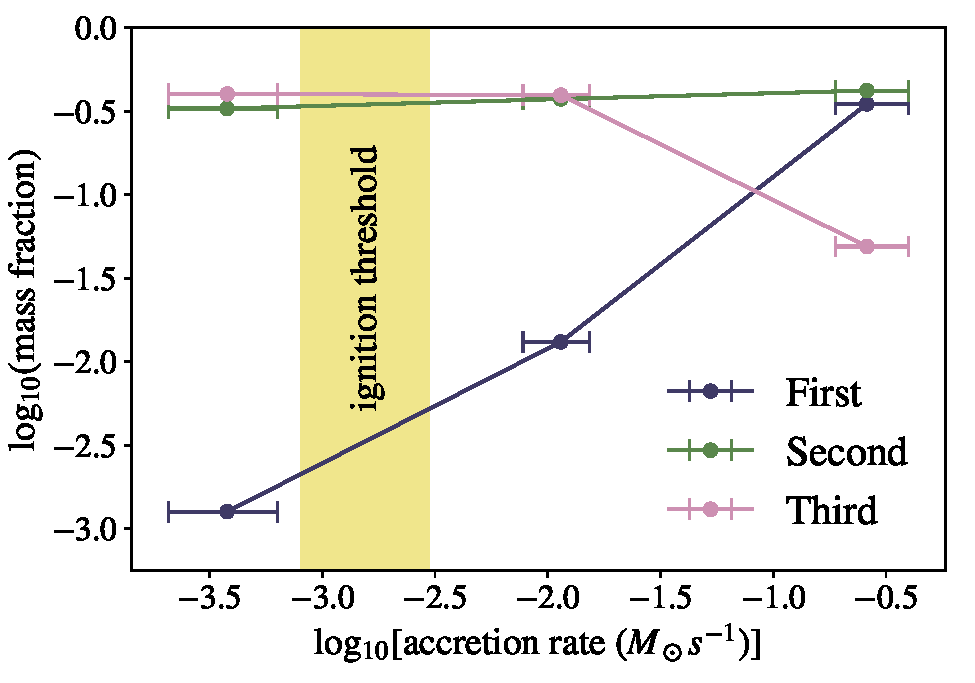
\includegraphics[width=\columnwidth]{figures/kilonova/mass_fraction_peaks.pdf}
 \caption{Mass fractions of the nucleosynthetic yields in
the first (summed over $A=70-90$), second (summed over $A=125-135$), and third (summed over $A=186-203$) r-process peaks for the disk ejecta of simulation runs \texttt{MD\_M03}, \texttt{MD\_M002}, and \texttt{MD\_M0002} presented here. A qualitative change in nucleosynthesis products across the ignition threshold for weak interactions (Eq.~\eqref{eq:Mdot_ign_merger}) is evident. \label{fig:mass_frac_peaks}}
\end{figure}

\begin{figure}[t]
  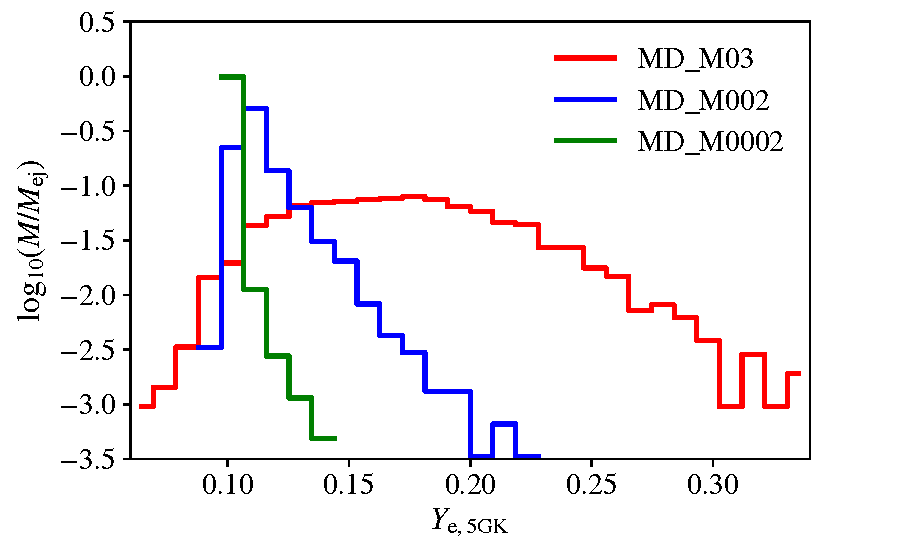
\includegraphics[width=\columnwidth]{figures/kilonova/Ye_sims_comparison_MD_M03-MD_M002-MD_M0002.pdf}
 \caption{Mass distribution of unbound outflows from our simulated accretion disks according to the electron fraction $Y_{\rm e}$, extracted from tracer particles at 5\,GK. A significant high-$Y_e$ tail is established across the ignition threshold. \label{fig:mass-Ye-outflow}}
\end{figure}

The neutron-rich outflows generated by our post-merger accretion disks are sites for r-process nucleosynthesis. We record thermodynamic properties of the ejecta by tracer particles distributed throughout the disks initially (cf.~Sec.~\ref{sec:ejecta}), and use such tracer profiles as input to nuclear reaction network calculations. The initial conditions important to the outcome of the r-process are set mostly by the electron fraction, specific entropy, and expansion timescale of the flow at $T\approx 5$\,GK \cite{lippuner_r-process_2015}, which is the characteristic temperature at which nuclear statistical equilibrium breaks down, and neutron-capture reactions set in.

Neutrino absorption is taken into account approximately by a ring-like `light-bulb' scheme in post-processing \cite{fernandez_delayed_2013}, which irradiates the ejecta with neutrino luminosities as computed in Sec.~\ref{sec:neutrino_emission}. We refer to Ref. \cite{fernandez_delayed_2013} and Ref. \cite{Siegel:2017jug} for more details on this approach.

Starting at 10~GK, we perform full nuclear reaction network calculations on the tracer particles using the reaction network \texttt{SkyNet}~\cite{lippuner_skynet:_2017}, in order to track nuclear abundances as the outflows undergo r-process nucleosynthesis. Figure \ref{fig:abundances} shows the final total abundance yields from all tracers after $10^9$\,s for all three disk simulation runs. These abundances are the result of integrated ejecta that are unbound over the course of the simulation runs, most of which originate from the inner accretion disk region with radii between $\approx(100-250)$~km (cf.~Fig.~\ref{fig:outflows}). 

Final r-process abundance patterns qualitatively change across the ignition threshold for weak interactions in post-merger disks (see Fig.~\ref{fig:abundances}). At high accretion rates, such as run \texttt{MD\_M03}, we find abundances in good agreement with residual solar r-process abundances~\cite{arnould_$r$-process_2007} across the entire range of mass numbers from the first ($A\approx80$) to the third ($A\approx195$) r-process peak (see \cite{Siegel:2017jug} for a more detailed discussion on this case). While across all accretion rates we find good agreement with the solar abundance pattern between the second peak ($A\approx130$) and the third r-process peak, run \texttt{MD\_M002} (close to the ignition threshold) already shows somewhat suppressed first-to-second peak elements, and light r-process elements are strongly suppressed below the ignition threshold (run \texttt{MD\_M0002}).

The qualitative change in nucleosynthesis patterns across the ignition threshold is further illustrated by Fig.~\ref{fig:mass_frac_peaks}, which shows the mass fractions of nuclei grouped into first-, second- and third-peak elements as a function of accretion rate. While 2nd-peak elements are synthesized in roughly constant amounts across the $\dot{M}$ range investigated here, abundances of light r-process nuclei rise strongly toward and around the ignition threshold, while 3rd-peak nuclei are somewhat overproduced in that regime.

This behavior is a result of a qualitative change in the distribution of $Y_e$ of the ejecta across the ignition threshold as evident from Fig.~\ref{fig:mass-Ye-outflow}. While at low $\dot{M}$, below the ignition threshold, the $Y_e$ distribution of the unbound outflows at 5\,GK is still centered around the initial value of $Y_e=0.1$ (run \texttt{MD\_M0002}), run \texttt{MD\_M002} close to the ignition threshold has already built up a significant tail toward higher electron fraction; finally, run \texttt{MD\_M03} shows a broad distribution of $Y_e$ at least up to $\lesssim 0.4$. This effect can be  ascribed in part to the strongly changing protonization timescale as a function of accretion rate across the ignition threshold (cf.~Eq.~\eqref{eq:t_Ye_scale_Mdot}; Sec.~\ref{sec:disk_composition}). There is a possibility of our tracer particles slightly under-resolving the high-$Y_e$ tail---a significantly larger number of tracers, excluded here due to computational cost and feasibility, may better resolve the effects of, e.g., an inner high-$Y_e$ part of the \texttt{MD\_M0002} disk, but is unlikely to qualitatively change the  conclusion reached here. Toward high $\dot{M}$, neutrino absorption by the ejecta contributes to flattening the $Y_e$ distribution as well. This effect is already noticeable for \texttt{MD\_M03} and is expected to become more important at even higher $\dot{M}$ disks \cite{miller_full_2019-1}, which are beyond the scope of the present paper.



%The nucleosynthetic yields of the three models can be understood with the help of Figure \ref{fig:panels_Ye_eta} and Figure \ref{fig:mass-Ye-outflow}. Figure \ref{fig:mass-Ye-outflow} shows the mass distribution of unbound outflows measured by tracer particles in terms of $Y_{\rm e}$. Ejecta from all three models can be seen to be comprised of significant amounts low $Y_{\rm e}$ material, $\approx(0.1-0.15)$, due to the initial disks being set to $Y_{\rm e} = 0.1$. % for a significant part in the outflows over time.
%For \texttt{MD\_M03} and \texttt{MD\_M002} this low $Y_{\rm e}$ material is generated from the inner disks, and for \texttt{MD\_M0002} from the outer disk, as observed in Figure \ref{fig:panels_Ye_eta}. As low $Y_{\rm e}$ corresponds to large number of free neutrons, this outflow material enables the $r$-process to generously produce high mass number nuclei. As the disk mass is increased, the ejecta can be seen to be spanning over of a broader range of $Y_{\rm e}$ material, such that the average values of $Y_{\rm e}$ is 0.101~erg s$^-1$ for \texttt{MD\_M0002}, 0.114~erg s$^-1$ for \texttt{MD\_M002}, and 0.174~erg s$^-1$ for \texttt{MD\_M03}.

%For \texttt{MD\_M03}, there is significant amount of neutrino production in the disk midplane. These neutrinos further change the composition of a part of the outer disks and the outflows, resulting in the addition sufficient high $Y_{\rm e}$ material--- corresponding to low mass nuclei---as well in the outflows. High $Y_{\rm e}$ implies availability of few amounts of free neutrons, disabling the $r$-process from producing high mass nuclei.

%For \texttt{MD\_M002}, the reduced amount of neutrino emission in the disk midplane, due to a lower accretion rate compared to \texttt{MD\_M03}, does not sufficiently change the composition of the outflows. The reduced conversion of low $Y_{\rm e}$ material to high $Y_{\rm e}$ material reduces the amount of production of low mass nuclei.

%For \texttt{MD\_M0002}, although the inner disk produces high $Y_{\rm e}$ material, they are not produced in significant amounts. The weak interactions in the inner disk in this model is not efficient enough to contribute strongly to the production of low mass nuclei. Additionally, neutrino emission being nearly absent in the disk midplane leads to a negligible conversion of low $Y_{\rm e}$ material produced by the outer disk to high $Y_{\rm e}$ material. These reasons combined explains the significant drop in the production of low mass nuclei, by about an order of magnitude lower as compared to \texttt{MD\_M002}.   


%Lots of n rich material, lots of lanthanides in lowest $\dot M$. How much ejecta do we get in the three cases?

%How much elements in each peak?

%Do we get/not get blue kilonova?

%Nucleosynthesis trends in second and third peaks.

%Do we get blue ejecta at all in MD\_M0002? Here, it'll come from the inner part.

%As we cross ignition threshold, we see where blue/red component is coming from.

%Blue ejecta component from outside, red component from inside.


%\section{Section 4}
%High velocity tail discussion. Which plots here?

%\section{Section 5}
%Summarize results in terms of future mergers.

\section{Conclusion}
\label{sec:conclusion}

%Discussion in the light of GW190425: low-mass accretion disks expected! Discuss disk outflow/mass in comparison with other ejecta channels for such high-mass NS-NS systems. Can we predict any kilonova estimates (would need kilonova model, will require extra work)?

Our simulation results provide important implications for the electromagnetic counterpart observables of LIGO-Virgo's source population BNS and NSBH mergers. As presented in Section \ref{sec:nucleosynthesis}, all three of our models produce heavy $r$-process elements---corresponding to red kilonova components, with our highest disk model being able to produce light $r$-process elements as well. Our results indicate that nucleosynthetic yields from postmerger accretion disks comprising primarily of light $r$-process elements, corresponding to a strong blue kilonova would require fairly high disk masses, such as the model in Ref. \cite{miller_full_2019-1}. As shown in Section \ref{sec:param_space}, high disk masses would result from small total masses for binary systems. The observation of a blue kilonova would be possible from very low mass BNS systems, and is unlikely from NSBH systems. The second LIGO-Virgo BNS detection, GW190425, was not accompanied by any electromagnetic counterparts. However, with binary total mass being one of the parameters that is accurately measured by gravitational-wave observations, this binary has been concluded to belong to the high mass regime of the neutron star binary parameter space. In such a scenario, our simulation results predict production of heavy $r$-process elements in the nucleosynthetic yields of the remnant accretion disks, resulting in a red kilonova. The system being located at significantly larger distances compared to the first BNS candidate, GW170817, in addition to the poor sky localization of the event, would account for the inability in detecting the kilonova signatures. 

\section{Appendix}
\subsection{Ignition threshold}
\label{app:ignition_threshold}

The basic scaling $\dot{M}_{\rm ign}\propto \alpha_{\rm visc}^{5/3}$ (cf.~Eq.~\eqref{eq:Mdot_ign}) of the accretion rate at the ignition threshold for weak interactions in an accretion disk with the dimensionless, effective Shakura-Sunyaev viscosity coefficient $\alpha_{\rm visc}$ can be derived analytically. To this end, we work within a height-integrated, one-dimensional model for accretion disks in Kerr spacetime with metric $g_{\mu\nu}$ using Boyer-Lindquist coordinates $x^i = (t,r,\theta, \phi)$ (e.g., \cite{beloborodov_super-eddington_1998,gammie_advection-dominated_1998,chen_neutrino-cooled_2007}). In such 1D models, angular averages are performed by approximating $\int {\rm d}\theta {\rm d}\phi \sqrt{g} q \simeq 4\pi H q(\theta = \pi/2)$, where $q$ represents any physical quantity, $H(r)$ is the characteristic angular half-thickness of the disk, and $g = {\rm det}(g_{\mu\nu})$. We work in the ``thin-disk'' approximation \cite{shakura_black_1973,bardeen_rotating_1972,novikov_astrophysics_1973}, well justified if neutrino cooling is significant, in which terms in $(H/r)^2$ are neglected and gas pressure is negligible, resulting in the assumption that the fluid orbits with four-velocity $u^\mu = (u^t,u^r, 0, u^\phi)$ and Keplerian angular velocity $\Omega \equiv u^\phi/u^t = c/(r\sqrt{2r/r_{\rm g}} + \chi_{\rm BH} r_{\rm g}/2)$. Here, $r_{\rm g}=2GM/c^2$ is the gravitational radius, and $M_{\rm BH}$ and $\chi_{\rm BH}$ denote, as before, the mass and the dimensionless spin of the black hole, respectively. In this thin-disk limit, the equation of vertical hydrodynamical equilibrium for the disk, can be written as (cf.~\cite{abramowicz_accretion_1997,beloborodov_super-eddington_1998})

\begin{equation}
	\left(\frac{H}{r}\right)^2 = \frac{2 r}{c^2 r_{\rm g} J(\chi_{\rm BH},r)}\frac{p}{\rho},\mskip40mu \text{or} \mskip40mu c_{\rm s} = c\left(\frac{J(\chi_{\rm BH},r) r_{\rm g}}{2r}\right)^{\frac{1}{2}}\frac{H}{r}, \label{eq:vertical_equilibrium}
\end{equation}

where $c_{\rm s}=\sqrt{p/\rho}$ is the isothermal sound speed, and
\begin{equation}
	J(\chi_{\rm BH},r) \equiv \frac{2\left(r^2 - \chi_{\rm BH} r_{\rm g}\sqrt{2r_{\rm g}r}+ 3\chi_{\rm BH}^2 r_{\rm g}^2 / 4 \right)}{2r^2 - 3r_{\rm g}r + \chi_{\rm BH} r_{\rm g}\sqrt{2r_{\rm g}r}}.
\end{equation}
The equation of baryon number conservation reads
\begin{equation}
	\dot{M} = -2\pi r c u^r \Sigma, \label{eq:baryon_conservation}
\end{equation}
where $\Sigma = 2H\rho$ is the disk surface density. From the equations of energy and angular momentum conservation, one can derive the identity \cite{page_disk-accretion_1974,chen_neutrino-cooled_2007}
\begin{equation}
	2\nu \Sigma r \sigma^{r}_\phi = -\frac{c r_{\rm g}}{4\pi} \dot{M} F(x,\chi_{\rm BH}), \label{eq:shear_identity}
\end{equation}
where $\nu$ is the kinematic viscosity, $\sigma^r_\phi = (1/2) c g^{rr} g_{\phi\phi}\sqrt{-g^{tt}}\gamma^3 ({\rm d}\Omega/{\rm d}r)$ is the shear, with $\gamma=u^t/\sqrt{-g^{tt}}$ being the Lorentz factor of the fluid measured by a zero-angular momentum observer, and
%\begin{eqnarray}

\begin{equation}
\begin{split}
F(x,\chi_{\rm BH}) \equiv \frac{x^3 + \chi_{\rm BH}}{(x^3 - 3x + 2\chi_{\rm BH})^{1/2}x^{3/2}} \Bigg[ (x-x_0)-\frac{3}{2}\chi_{\rm BH} \ln\frac{x}{x_0}- \\ \frac{3(x_1-\chi_{\rm BH})^2}{x_1(x_1-x_2)(x_1-x_3)}\ln\left(\frac{x-x_1}{x_0-x_1}\right) - \frac{3(x_2-\chi_{\rm BH})^2}{x_2(x_2-x_1)(x_2-x_3)}\ln\left(\frac{x-x_2}{x_0-x_2}\right) - \\ \frac{3(x_3-\chi_{\rm BH})^2}{x_3(x_3-x_1)(x_3-x_2)}\ln\left(\frac{x-x_3}{x_0-x_3}\right)\Bigg]. \label{eq:F_x}
\end{split}
\end{equation}
%\end{eqnarray}

Here, $x\equiv \sqrt{2r/r_{\rm g}}$, $x_0$ corresponds to the location of the marginally stable orbit, and $x_1$, $x_2$, $x_3$ are the roots of $x^3-3x+2\chi_{\rm BH}=0$. Explicitly, $x_1=2\cos(\frac{1}{3}\cos^{-1}\chi_{\rm BH}-\pi/3)$, $x_2=2\cos(\frac{1}{3}\cos^{-1}\chi_{\rm BH}+\pi/3)$, and $x_3=-2\cos(\frac{1}{3}\cos^{-1}\chi_{\rm BH})$.
Substituting Eq.~\eqref{eq:shear_identity} into Eq.~\eqref{eq:baryon_conservation} and using Eq.~\eqref{eq:vertical_equilibrium} one finds
\begin{equation}
	u^r = \frac{8}{3} \left(\frac{J(r,\chi_{\rm BH}) r}{2c^2 r_{\rm g}}\right)^{\frac{1}{2}} \frac{\sigma^r_\phi}{F(x,\chi_{\rm BH})}\alpha \left(\frac{H}{r}\right)^2, 
\end{equation}
where we have adopted the Shakura-Sunyaev parametrization $\nu = \frac{2}{3}\alpha_{\rm visc} c_{\rm s} H$ with viscosity coefficient $\alpha_{\rm visc}$. Substituting this back into Eq.~\eqref{eq:baryon_conservation}, we obtain
\begin{eqnarray}
	\dot{M} &=& - \frac{32\pi r_{\rm g}^2}{3\sqrt{2}} J^{\frac{1}{2}}(r,\chi_{\rm BH}) \left(\frac{r}{r_{\rm g}}\right)^{\frac{5}{2}} \frac{\sigma^r_\phi}{F(x,\chi_{\rm BH})}\alpha \rho \left(\frac{H}{r}\right)^3  \label{eq:Mdot_1D_1} \\
		&=& 2\sqrt{2}\pi c r_{\rm g}^2 S^{-1}(r,\chi_{\rm BH}) J^{\frac{1}{2}}(r,\chi_{\rm BH})  \left(\frac{r}{r_{\rm g}}\right)^{\frac{3}{2}} \alpha \rho \left(\frac{H}{r}\right)^3,  \label{eq:Mdot_1D_2}
\end{eqnarray}
where we have introduced the function $S(r,\chi_{\rm BH})=-(3/8)c(r_{\rm g}/r) [F(x,
\chi_{\rm BH})/\sigma^r_\phi]$, which varies between zero at the marginally stable orbit $x_0$ and unity at $r\rightarrow\infty$.

Viscous heating rate per unit area of the disk is given by $Q^+ = 2\nu\Sigma h c \sigma^r_\phi \sqrt{-g^{tt}}\gamma ({\rm d}\Omega/{\rm d}r)$, where $h\approx 1$ is the specific enthalpy of the fluid in the thin disk \cite{beloborodov_super-eddington_1998}. Using the identity \eqref{eq:shear_identity} one can rewrite this as
\begin{equation}
	Q^+ = \frac{c^2}{4\pi}\left(\frac{r}{r_{\rm g}}\right)^{-1} F(x,\chi_{\rm BH}) \mathcal{Q}(r,M_{\rm BH},\chi_{\rm BH}) \dot{M}, \label{eq:Qplus}
\end{equation}
where $\mathcal{Q}(r,M_{\rm BH},\chi_{\rm BH})\equiv -u^t ({\rm d}\Omega/{\rm d}r)$. We assume that cooling of the disk is dominated by electron and positron capture (URCA cooling). Ignoring final state blocking in the neutrino phase space, the cooling rate per unit area of the disk is then approximately given by \cite{tubbs_neutrino_1975,Bruenn:1985en,qian_nucleosynthesis_1996,popham_hyperaccreting_1999}
\begin{equation}
	Q^-_\nu = 2H \mathcal{C}_\nu \rho T^6. \label{eq:Qminus_nu_def}
\end{equation}
Here, $\mathcal{C}_\nu$ is a constant times the mass fraction of nucleons $X_{\rm nuc}$, which is roughly unity in the inner parts of the accretion disk where photodisintegration breaks down nuclei into neutrons and protons once $T\sim 10^{10}$\,K. At sufficiently small $\dot{M}$ (low midplane density), the pressure is dominated by radiation pressure, $p = \frac{11}{12}a_{\rm SB} T^4$, where contributions of relativistic electron-positron pairs have been included \cite{popham_hyperaccreting_1999}. Substituting into Eq.~\eqref{eq:vertical_equilibrium}, this yields the disk midplane temperature
\begin{equation}
	T = \left(\frac{6}{11}\frac{c^2}{a_{\rm SB}}\right)^{\frac{1}{4}} J^{\frac{1}{4}}(r,\chi_{\rm BH}) \left(\frac{r}{r_{\rm g}}\right)^{-\frac{1}{4}} \left(\frac{H}{r}\right)^{\frac{1}{2}} \rho^{\frac{1}{4}}. \label{eq:T_1D}
\end{equation}
Using this relation in Eq.~\eqref{eq:Qminus_nu_def} together with Eq.~\eqref{eq:Mdot_1D_2}, one obtains the following expression for neutrino cooling:
\begin{equation}
	Q^-_\nu = 2 \mathcal{C}_\nu \left(\frac{1}{2\sqrt{2}\pi c}\right)^{\frac{5}{2}} \left(\frac{6}{11}\frac{c^2}{a_{\rm SB}}\right)^{\frac{3}{2}} r_{\rm g}^{-4} S^{\frac{5}{2}}(r,\chi_{\rm BH}) J^{\frac{1}{4}}(r,\chi_{\rm BH}) \left(\frac{r}{r_{\rm g}}\right)^{-\frac{17}{4}}\left(\frac{H}{r}\right)^{-\frac{7}{2}} \alpha^{-\frac{5}{2}}\dot{M}^{\frac{5}{2}}. \label{eq:Qminus_nu}
\end{equation}

Adopting the condition $Q^-_\nu/Q^+ = 1/2$ for weak interactions to become energetically significant, one can employ the expressions \eqref{eq:Qplus} and \eqref{eq:Qminus_nu} to formulate this as a condition on the accretion rate:

\begin{eqnarray}
%\begin{adjustwidth}{-1mm}{}
\dot{M}_{\rm ign} = \left(\frac{c^2}{16\pi \mathcal{C}_\nu }\right)^{\frac{2}{3}} \left(2\sqrt{2}\pi c\right)^{\frac{5}{3}} \left(\frac{11}{6}\frac{a_{\rm SB}}{c^2}\right)^{\frac{5}{3}} r_{\rm g}^{\frac{8}{3}} S^{-\frac{5}{3}} J^{-\frac{1}{6}}F^{-\frac{2}{3}} \mathcal{Q}^{-\frac{2}{3}}\left(\frac{r}{r_{\rm g}}\right)^{\frac{13}{6}}\left(\frac{H}{r}\right)^{\frac{7}{3}} \alpha^{\frac{5}{3}}. \\
\equiv \dot{\mathcal{M}}_{\rm ign}(r,M_{\rm BH},\chi_{\rm BH}) \alpha^{\frac{5}{3}}.
%\end{adjustwidth}
\end{eqnarray}

where $\dot{\mathcal{M}}(r,M_{\rm BH},\chi_{\rm BH})$ is a function that depends on the black-hole parameters. Except for $S(r)$, which must be calculated numerically (but can be approximated analytically), $\dot{\mathcal{M}}(r,M_{\rm BH},\chi_{\rm BH})$ can be analytically evaluated on a horizon-scale $r\sim r_{\rm g}$ to provide the characterisitic accretion rate onto the black hole.

\Chapter{Conclusions}
\label{ch:conclusions}
In the current era of gravitational-wave astrophysics we are moving beyond first direct detections and first multimessenger observations, to now making routine discoveries that deepen our understanding of the compact objects in our cosmic neighborhood. The LIGO-Virgo gravitational-wave detector network has detected 52 confirmed binary merger observations so far, and the detection rate has only accelerated as improved detector sensitivity extends our reach deeper into the universe. From the two observed binary neutron star mergers, our knowledge of the dynamics of these events and of neutron star physics has grown dramatically. They have provided confirmation of binary neutron star mergers as a source of short gamma-ray bursts, and also as important sites of heavy element production through $r$-process nucleosynthesis that can help explain observed chemical abundances. They have also shown that it is possible to measure the tidal information in a gravitational-wave signal to meaningfully update our constraints on the nuclear equation of state. As the LIGO-Virgo detectors approach their design sensitivity, and as third-generation detectors begin to come online, we expect to see many more binary neutron star mergers in the coming years. We anticipate that these new detections will provide even further insights into the physics of neutron stars.

In this thesis we have studied binary neutron star mergers, through a combination of observations and computational modeling. Specifically we explore the ability of a gravitational-wave analysis to extract physical parameters of the binary system, and of the neutron stars involved in the merger. We investigate the impact of multimessenger information on a gravitational-wave analysis, and we study the measurability of the nuclear equation of state, both now and in the future.

We have presented an analysis of the binary neutron star merger GW170817 informed by electromagnetic distance measurements of its identified host galaxy, and we demonstrated that using an independent distance measurement in a gravitational-wave analysis can break the distance-inclination degeneracy to allow for much tighter constraints on the inclination angle of the binary. We find our improved measurement of the inclination supports models for a structured relativistic jet and its afterglow emission being viewed off-axis.

We have presented measurements of the tidal deformabilities and radii of the neutron stars in GW170817. Our analysis imposed a physical constraint to require that both neutron stars obey the same equation of state, and we used a prior on the leading order tidal parameter constructed to contain all physical models of the equation of state without biasing the measurement toward any particular model. We note that the methodology we employed could be adapted for the analysis of future binary neutron star merger events with similar masses. We find our results are broadly consistent with several other studies~\cite{Abbott:2018exr,Radice:2018ozg,Coughlin:2018fis,Capano:2019eae} which employed various methods to measure the tidal deformabilities and radii in their own analyses of GW170817.

We have presented a likelihood model developed for \textit{PyCBC Inference} that uses the relative binning parameter estimation technique to reduce computational cost for potential multimessenger gravitational-wave sources. We extended the work of previous implementations to make our relative likelihood model a coherent network statistic so that it can additionally measure sky locations. We validated the relative model on populations of simulated binary neutron star and simulated neutron star--black hole merger signals, and we showed that it is possible to seed the relative analysis with the best-fit template parameters from a low-latency search pipeline. We found that the parameter estimation for all signals in our simulated populations completed in less than 20 minutes, with sky localization and intrinsic parameter estimates that are comparable to analyses done with a standard non-relative likelihood.

We have presented a comprehensive study of the future prospects for a precise equation of state measurement from Advanced LIGO and Cosmic Explorer. We explored the measurability of the equation of state across the full parameter space allowed by combined constraints from astrophysical observations and nuclear experiments. We showed that a precision threshold for measurements to distinguish between substantially similar theoretical models for the equation of state is equivalent to measuring the radius of a 1.4\msun\ neutron star to better than $2\%$, and we presented a framework for combining individual equation of state measurements across entire populations to produce a combined, high-precision measurement. We found it is unlikely that Advanced LIGO will achieve $2\%$ precision in the next observing runs given current estimates of the merger rate for binary neutron stars, however Cosmic Explorer will measure the equation of state to better than $1\%$ within one year of operation. Our framework can be directly applied to any future signals from binary neutron star mergers, and we anticipate that the resulting precise knowledge of the true equation of state will be invaluable for efforts to model these merger events and their associated kilonovae.
%\appendix
%\chapter{}
%\label{}
%\input{}
\clearpage
\bibliographystyle{unsrt}
\bibliography{o2_bbh_pe_bib,common_eos_bib,common_envelope_bib,MyLibrary,kilonova_bib,einsteintoolkit,additional_references}
\addcontentsline{toc}{chapter}{\numberline {Bibliography}}

\renewenvironment{thebibliography}[1]%
  {\begin{list}{\labelenumi\hss}%
     {\usecounter{enumi}\setlength{\labelwidth}{3em}%
      \setlength{\leftmargin}{5em}}}%
  {\end{list}}
\renewcommand{\bibitem}[1]{\item\label{#1}\relax}%
\renewcommand{\theenumi}{\arabic{enumi}}%
%\fi
%\clearpage
%\newpage
%%%%%%%%%%%%%%%%%%%%%%%%%%%%%%%%%%%%%%%%%%%%%%%%%%%%%%%%%%%%%%%%%%%%%%%
% LaTeX Template: Curriculum Vitae
%
% Source: http://www.howtotex.com/
% Feel free to distribute this template, but please keep the
% referal to HowToTeX.com.
% Date: July 2011
% 
%%%%%%%%%%%%%%%%%%%%%%%%%%%%%%%%%%%%%%%%%%%%%%%%%%%%%%%%%%%%%%%%%%%%%%
% How to use writeLaTeX: 
%
% You edit the source code here on the left, and the preview on the
% right shows you the result within a few seconds.
%
% Bookmark this page and share the URL with your co-authors. They can
% edit at the same time!
%
% You can upload figures, bibliographies, custom classes and
% styles using the files menu.
%
% If you're new to LaTeX, the wikibook is a great place to start:
% http://en.wikibooks.org/wiki/LaTeX
%
%%%%%%%%%%%%%%%%%%%%%%%%%%%%%%%%%%%%%%%%%%%%%%%%%%%%%%%%%%%%%%%%%%%%%%

%%% Macros
%%% ------------------------------------------------------------
\newlength{\spacebox}
\settowidth{\spacebox}{8888888888}			% Box to align text
\newcommand{\sepspace}{\vspace*{1em}}		% Vertical space macro

\newcommand{\MyName}[1]{% Name
		\normalsize \usefont{OT1}{phv}{b}{n} \hfill #1
		\par \normalsize \normalfont}
		
\newcommand{\NewPart}[1]{\section*{#1}}

\newcommand{\PersonalEntry}[2]{
		\noindent\hangindent=2em\hangafter=0 % Indentation
		\parbox{\spacebox}{        % Box to align text
		\textit{#1}}		       % Entry name (birth, address, etc.)
		\hspace{1.5em} #2 \par}    % Entry value

\newcommand{\SkillsEntry}[2]{      % Same as \PersonalEntry
		\noindent\hangindent=2em\hangafter=0 % Indentation
		\parbox{\spacebox}{        % Box to align text
		\textit{#1}}			   % Entry name (birth, address, etc.)
		\hspace{1.5em} #2 \par}    % Entry value	
		
\newcommand{\EducationEntry}[4]{
		\noindent \textbf{#1} \hfill      % Study
		\noindent \textbf{#2} \par
        \noindent \textit{#3} \par        % School
		\noindent\hangindent=2em\hangafter=0 \small #4 % Description
		\normalsize \par}

\newcommand{\WorkEntry}[4]{				  % Same as \EducationEntry
		\noindent \textbf{#1} \hfill      % Jobname
		\noindent \textbf{#2} \par  % Duration
		\noindent \textit{#3} \par              % Company
		\noindent\hangindent=2em\hangafter=0 \small #4 % Description
		\normalsize \par}
		
\newcommand{\HonorsEntry}[4]{				  % Same as \EducationEntry
		\noindent \textbf{#1} \hfill     % Jobname
		\noindent \textbf{#2} \par  
		\noindent \textit{#3} \par % Company
		\noindent\hangindent=2em\hangafter=0 \small #4 % Description
		\normalsize \par}

\newcommand{\ContributedTalksEntry}[3]{
         \noindent \textbf{#1} \hfill % Talk Title
         \noindent \textbf{#2} \par % Year
         \noindent\hangindent=2em\hangafter=0 \small #3 % Description
		 \normalsize \par
         }

\newcommand{\PublicationsEntry}[1]{
        \noindent #1 \par}

\newcommand{\Outreach}[3]{
        \noindent \textbf{#1} \hfill
        \noindent \textbf{#2} \par
        \noindent\hangindent=2em\hangafter=0 \small #3 % Description
		\normalsize \par}

%%% Begin Document
%%% ------------------------------------------------------------
\begin{document}

% you can upload a photo and include it here...
%\begin{wrapfigure}{l}{0.5\textwidth}
%	\vspace*{-2em}
%		\includegraphics[width=0.15\textwidth]{photo}
%\end{wrapfigure}

\MyName{Steven Reyes}

\sepspace

%%% Personal details
%%% ------------------------------------------------------------
\NewPart{Personal details}{}

\PersonalEntry{Citizenship}{United States of America}
\PersonalEntry{Birth}{May 4, 1992}
%\PersonalEntry{Address}{413 Roosevelt Ave, Syracuse, NY 13210}
\PersonalEntry{Phone}{(773) 315-2296}
\PersonalEntry{Mail}{\url{stevereyes01@gmail.com}}

%%% Education
%%% ------------------------------------------------------------
\NewPart{Education}{}

\EducationEntry{Syracuse University}{2014-Present}{Doctor of Philosophy in Physics}
{Advisor: Dr. Duncan Brown.
 \newline
 Expected Graduation date: 2019}
\sepspace

\EducationEntry{University of Chicago}{2010-2014}{Bachelor of Arts in Physics with Astrophysics specialization}{}

%%% Work experience
%%% ------------------------------------------------------------
\NewPart{Employment}{}

\WorkEntry{Graduate Student Research Assistant}{2015-Present}{Syracuse University, Advisor: Dr. Duncan Brown}{}
\sepspace

\WorkEntry{CARMA data analyst}{2012-2013}{University of Chicago, Advisor: Dr. John Carlstrom}{}

%%% Honors and Awards
%%% ------------------------------------------------------------
\NewPart{Honors and Awards}{}
\HonorsEntry{Gruber Cosmology Prize}{2016}{The Gruber Foundation}{Shared with the LSC}
\HonorsEntry{Breakthrough Prize in Fundamental Physics}{2016}{}{Shared with the LSC}
\HonorsEntry{STEM Fellowship}{2014, 2016}{Syracuse University}{}
\sepspace
\HonorsEntry{Odyssey Scholarship}{2010-2014}{University of Chicago}{}
\sepspace
\HonorsEntry{Chicago Public School (CPS) Scholarship}{2010-2014}{University of Chicago}{}


%%% Publications
%%% ------------------------------------------------------------
\NewPart{Publications in which Steven Reyes made a significant contribution}{
     \noindent \textit{}
     \newline \par
     \noindent Nitz, Alexander H and Capano, Collin and Nielsen, Alex
                        B. and Reyes, Steven and White, Rebecca and Brown, Duncan
                        A. and Krishnan, Badri. ``1-OGC: The first open gravitational-wave catalog of
                        binary mergers from analysis of public Advanced LIGO
                        data". In: (2018). arXiv:1811.01921 \texttt{[gr-qc]}
     \newline \par
     \noindent Steven Reyes and Duncan A. Brown ``Constraints on nonlinear tides due to $p$-$g$
               mode coupling from the neutron-star merger GW170817". In: (2018). arXiv: 1808.07013 \texttt{[astro-ph.HE]}
     \newline \par
     \noindent Nitz, Alexander H. and Dal Canton, Tito and Davis, Derek
                        and Reyes, Steven ``Rapid detection of gravitational waves from compact binary
                        mergers with PyCBC Live". In: \textit{Phys. Rev.} D98.2 (2018), p. 024050. \texttt{DOI: 10.1103/PhysRevD.98.024050}. arXiv: 1805.11174 \texttt{[gr-c]}
     \newline \par
     \noindent Benjamin P. Abbott et al. ``Upper Limits on the Rates of Binary Neutron Star and Neutron Star Black Hole
               Mergers From Advanced LIGO's First Observing Run". In: \textit{Astrophys. J.} 832.2 (2016), p. L21.
               \texttt{DOI: 10.3847/2041-8205/832/2/L21}. arXiv: 1607.07456 \texttt{astro-ph.HE}

     }

%%% Contributed Talks
\NewPart{Contributed Talks and Posters}{}
\ContributedTalksEntry{Searching for p-g mode coupling in GW170817}{2019}{Talk at STAG Research Centre (South Hampton, United Kingdom)}
\ContributedTalksEntry{Model Selection with Mult-Tempering Techniques}{2019}{Talk at PyCBC Inference Conference (Portsmouth, United Kingdom)}
\ContributedTalksEntry{Searching for p-g mode coupling in GW170817}{2018}{Poster at GWPAW 2018 (College Park, Maryland)}
\ContributedTalksEntry{The Search for Gravitational Waves from Binaries with Neutron Stars}{2017}{Talk at GWPAW 2017 (Annecy, France)}
\ContributedTalksEntry{First Results from the Search for Binary Black Hole Coalescence
with Advanced LIGO}{2016}{Poster at Relativity and Gravitation: Contemporary Research and Teaching of Einstein's Physics, Gordon Research Conference.}

%%% Outreach
%%% ------------------------------------------------------------
\NewPart{Outreach}{}
\Outreach{Lead Tour Guide at Holden Observatory}{2015-Present}
{}

\Outreach{Adopt-a-Physicist participant}{2015, 2016}
{}

\Outreach{Scholastic Dinosaur 13 Webinar Interview}{2014}{}

\end{document}

\setboolean{@twoside}{false}
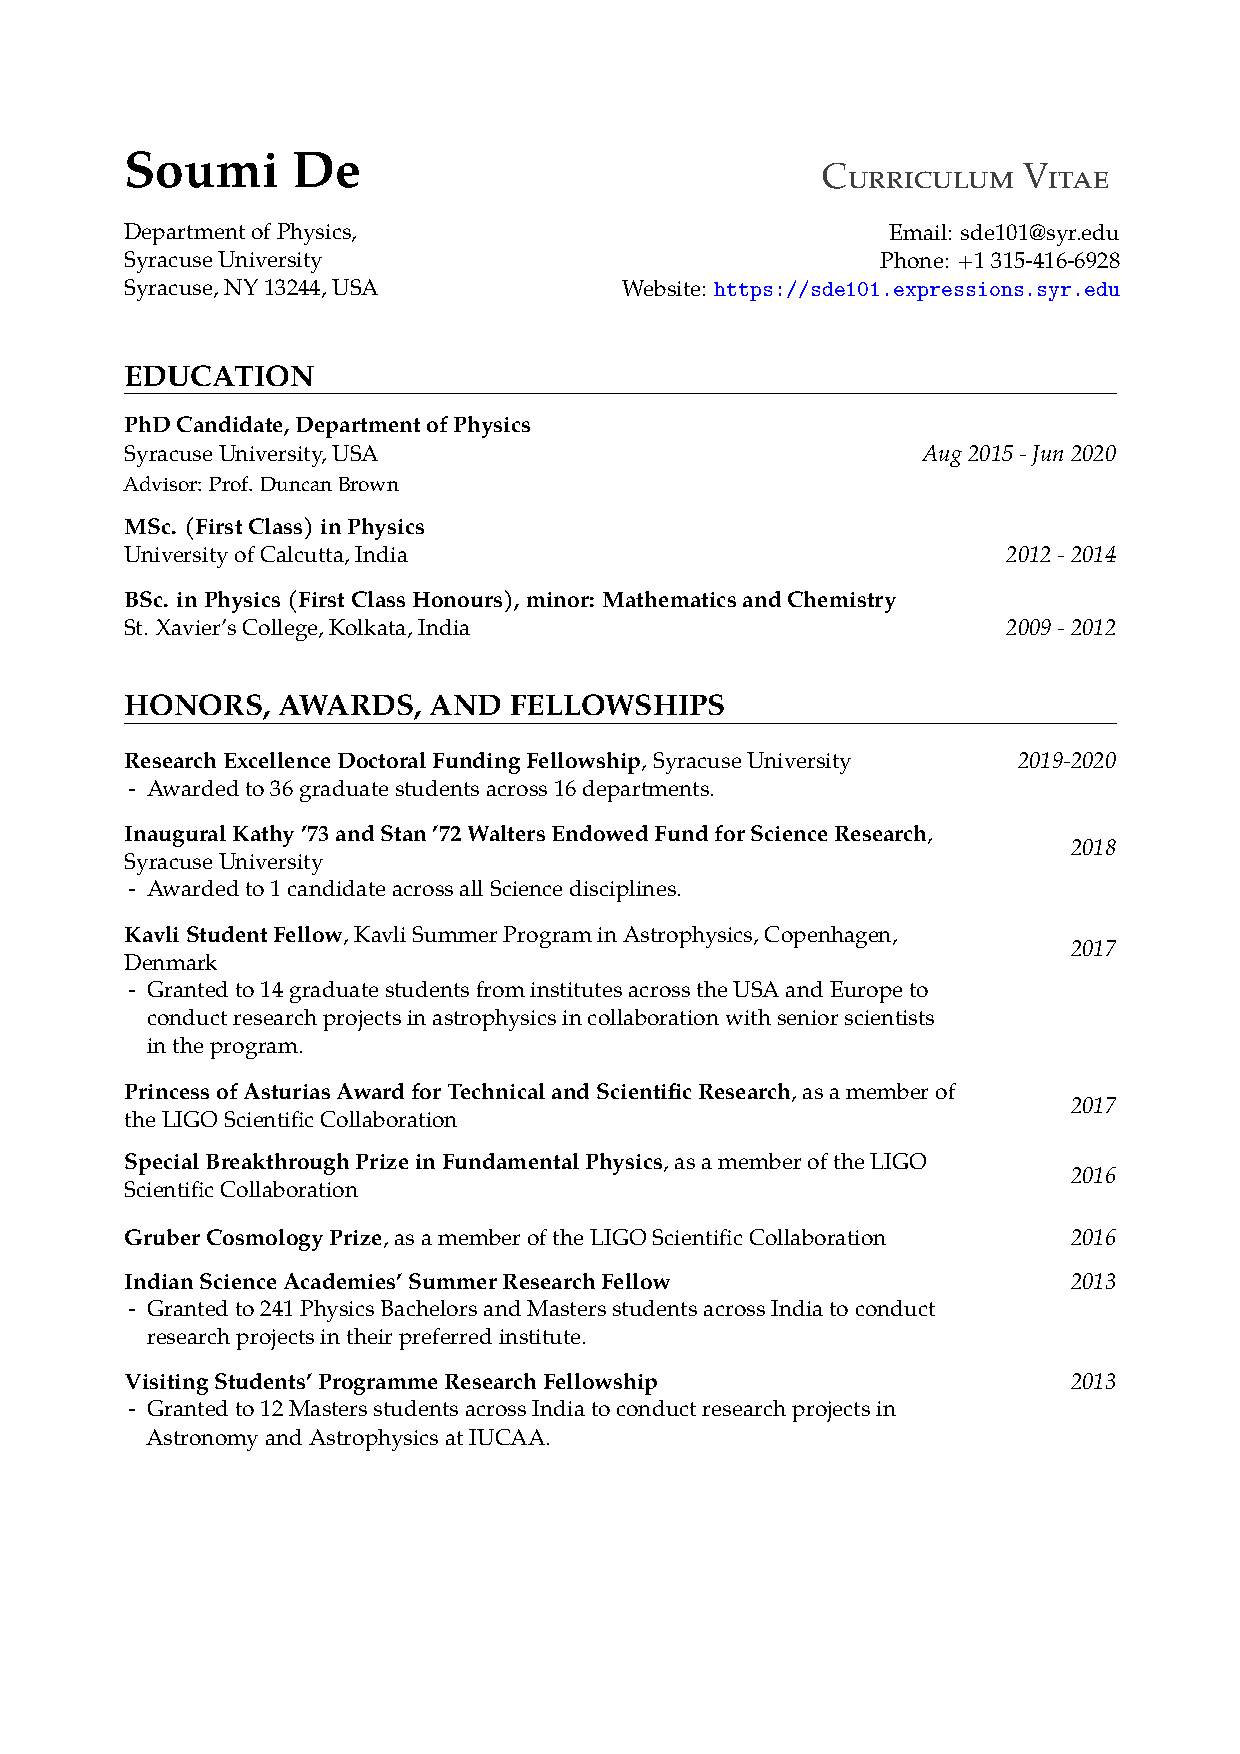
\includepdf[pages=-]{CV.pdf}

%\includepdf[pages=-, offset=25 -25]{Soumi_De_CV.pdf}

%\finishvita
% The grad school requires the last page to be blank
\newpage
\thispagestyle{empty}
\end{document}
